\documentclass[10pt,a4paper,twoside,fleqn]{book}
\usepackage{inchmargins,fancyhdr,amsmath,graphicx,moreverb,listings,color,crtitle}
%\usepackage{makeidx}
\usepackage{tocloft}
\usepackage{graphicx}
\usepackage[
    colorlinks=true,
    linkcolor=red,
    pdfpagemode=UseOutlines,
    pdfdisplaydoctitle=true,
    pdfpagelayout=SinglePage
]{hyperref}
\pagestyle{fancy}




%\newcommand{\fixdate}{24th July 2020}


\setcounter{secnumdepth}{2}

\newcommand{\htitle}{\bf 3PL Implementation}
\newcommand{\hauthor}{Paul Dunn}
\newcommand{\hdate}{30th July 2021}
\newcommand{\hreport}{Open report - CSIRO Mineral Resources}
%\newcommand{\hhead}{}
\newcommand{\hhead}{\leftmark}
\newcommand{\hfoot}{Open report - CSIRO Mineral Resources}



%\documentclass[12pt,a4paper,fleqn]{article}
%\usepackage{inchmargins,fancyhdr,epsfig,html}
%\pagestyle{fancyplain}
 
\def\fps@table{htbp}
%\def\topfraction{.9}
%\def\bottomfraction{.9}
%\def\textfraction{.1}
%\def\floatpagefraction{.9}
\renewcommand{\topfraction}{.95}
\renewcommand{\bottomfraction}{.95}
\renewcommand{\textfraction}{.05}
\renewcommand{\floatpagefraction}{.95}
\setlength{\mathindent}{2cm}
\setcounter{topnumber}{5}
\setcounter{bottomnumber}{5}
\setcounter{totalnumber}{10}
\newcommand{\blist}{\begin{list}{$\bullet$}{\setlength{\itemsep}{-5pt}\setlength{\topsep}{-5pt}}}
\newcommand{\blend}{\end{list}}
\newcommand{\autorefph}[1]{\autoref{#1} p\pageref*{#1}}

%\renewcommand{\section}{\@startsection
%                           {section}
%                           {1}
%                           {0mm}
%                           {-\baselineskip}
%                           {0.5\baselineskip}
%                           {\Large\bfseries}
%                       }
%\renewcommand{\subsection}{\@startsection
%                           {subsection}
%                           {2}
%                           {0mm}
%                           {-\baselineskip}
%                           {0.5\baselineskip}
%                           {\large\bfseries}
%                       }

\lstset{
    basicstyle=\small\ttfamily,
    basewidth={0.5em},
    tabsize=4,
    keywordstyle=\color{limegreen},
    commentstyle=\color{darkorchid},
    stringstyle=\color{darkviolet},
    showstringspaces=false
}
% set frames and line numbers for all further listings
\lstset{
    basicstyle=\footnotesize\ttfamily,
    basewidth={0.5em},
    frame=single,
    tabsize=4,
    numbers=left,
    numberstyle=\tiny,
    stepnumber=1,
    numbersep=5pt
}
    

\definecolor{orangered}{rgb}{0.99,0.27,0}
\definecolor{brown}{rgb}{0.64,0.16,0.16}
\definecolor{limegreen}{rgb}{0.19,0.76,0.19}
\definecolor{darkorchid}{rgb}{0.6,0.19,0.8}
\definecolor{darkviolet}{rgb}{0.58,0,0.82}

\lstloadlanguages{C}
\lstloadlanguages{Java}
\lstdefinelanguage{threepl} {
    morekeywords=[1]{value,selectvalue,queue,static,input,output,priority,clock,var,struct,int,float,str,log,cmemory,rmemory,type,enum,input,output,useclock},
    morekeywords=[2]{source,nosource,module,nomodule,procedure,function,global,local,calling,file,if,else,case,default,switch,while,do,for,seq,par,sync,when,break,return,unless},
    otherkeywords={<,>,=,<=,>=,\!=,==,<-,<<-,|-,:=,->},
    sensitive=true,
    keywordstyle=\color{orangered},
    keywordstyle=[1]\color{brown},
    keywordstyle=[2]\color{limegreen},
    commentstyle=\color{darkorchid},
    stringstyle=\color{darkviolet},
    morecomment=[l]{//},
    morecomment=[s]{/*}{*/},
    morestring=[b]"
}
\lstdefinelanguage{tde} {
    morekeywords={EXECP,DIVERGE,ILOOP,REG,QUEUE,WHEN,SELECT,DEL,QUEUEBUFFER,DO,WHILE,DFF},
    sensitive=true
}
%\lstdefinelanguage{java} {
%    morekeywords=[1]{void,Integer,int,Long,long,Boolean,boolean,Double,double,String,ArrayList,HashMap,HashSet},
%    morekeywords=[2]{public,private,abstract,class,extends,implements,static,final,if,else,case,default,switch,while,do,for,break,return,true,false,null},
%    otherkeywords={<,>,=,<=,>=,\!=,==},
%    sensitive=true,
%    keywordstyle=\color{orangered},
%    keywordstyle=[1]\color{brown},
%    keywordstyle=[2]\color{limegreen},
%    commentstyle=\color{darkorchid},
%    stringstyle=\color{darkviolet},
%    morecomment=[l]{//},
%    morecomment=[s]{/*}{*/},
%    morestring=[b]"
%}

% xfig diagrams -
% Helvetica-Narrow-Bold, size 8
% arrow type solid (3rd in menu), thickness 1.0, width 3.0, height 6.0


\renewcommand{\chaptermark}[1]{\markboth{#1}{}}
%\renewcommand{\sectionmark}[1]{\markright{#1}}

   
\setlength{\parskip}{3ex}
\setlength{\parindent}{0pt}
    

\begin{document}
     
%\maketitle
\makecsirotitle
  
\pagenumbering{roman}

\setlength{\parskip}{0pt}
\phantomsection
\pdfbookmark[0]{Contents}{\contentsname}
\tableofcontents
\setlength{\parskip}{0.6pc plus 0.2pc minus 0.2pc}

\cleardoublepage

\pagenumbering{arabic}
\setcounter{page}{1}



\chapter{Overview}

    3PL parses source code and produces a code tree, the root of which is {\bf
    ThreePL/main}. Leader, trailer and post-processing modules encountered during
    parsing are accumulated in lists {\bf leader\_modules}, {\bf trailer\_modules}
    and {\bf post\_modules}. All libraries are in source code form and are
    inserted into the source code via {\bf source} or {\bf module} statements.
    
    After parsing -
    \blist
    \item   The leader module list is traversed and each module is executed.
    \item   The code tree is then executed. Any target code generated during
            immediate execution is added to the intermediate code list {\bf
            ThreePL/tdelist}.
    \item   The trailer module list is traversed and each module is executed.
    \item   The intermediate code list is optimised and then traversed to
            generate netlist code to the EDIF file.
    \item   The post-processing module list is traversed and each module is
            executed to run vendor place-and-route tools.
    \blend


    \section{Operation}
    

        The main program is in source file ThreePL.java. The parser is in source
        file parser/Parser.jj which is processed by the Java compiler compiler
        Javacc to produce file Parser.java which is then compiled by the Java
        compiler.

        The main program reads and processes the command line arguments. If 3pl
        is called with no source file name, an interactive file chooser is then
        started from which the continuation of the main program can be called
        repeatedly. If there is a source file name, the continuation of the main
        program is called once only.
        \begin{lstlisting}[gobble=8, language=java]
            if (source_file == null) {
                // Start up a file chooser GUI which can repeatedly call
                // mainContinue().
                .
                .
                .
                .
                .
                file_chooser_used = true;
                fc = new FileChooser();
                FileChooser.display();
            } else {
                // Just continue execution - mainContinue().
                file_chooser_used = false;
                int ret = mainContinue();
                if (ret != 0)
                    System.exit(ret);
            }
        \end{lstlisting}
        
        After a great deal of initialisation the parser is called -
        \begin{lstlisting}[gobble=8, language=java]
            try {
                input_stream = new SrcReader(source_file);
            } catch (FileNotFoundException e) {
                msg("unable to open source file '" + source_file + "'");
                return(1);
            }
            try {
                if (parser == null)
                    parser = new Parser(input_stream); // first use
                else
                    Parser.ReInit(input_stream);        // subsequent uses
                main = Parser.Filemodule();
            } catch (ParseException e) {
                msg("");
                msg("Parse error: file '" + file_name + "' line " + line_no);
                msg(e.getMessage());
                return(1);
            } catch (TokenMgrError e) {
                msg("");
                msg("Parse error: file '" + file_name + "' line " + line_no);
                msg(e.getMessage());
                return(1);
            } catch (ExEx e) {
                msg("");
                msg("Compilation error");
                msg(e.getMessage());
                return(1);
            }
            input_stream.close();
        \end{lstlisting}
        
        The parser builds a code tree rooted at local variable {\bf main}. The
        root of the tree will be a module call ({\bf ProcModCallNode}) to a file
        module associated with the initial source file. During parsing any
        leader or trailer modules encountered will be added to the leader or
        trailer module list. Any parsing errors result in immediate termination
        with an appropriate message.

        Following parsing, any modules in the leader module list are executed by
        the interpreter. The file module in {\bf main} is then passed to the
        intereter for execution. Finally any modules in the trailer module list
        are executed by the interpreter. Execution of the parsed code by the
        interpreter is refered to as "immediate" execution to distinguish it
        from later execution of target code in the FPGA. Most errors encountered
        during immediate execution result in termination with an error message.

        As immediate execution proceeds, any statements which produce target
        code will add elements to the intermediate code list. These elements
        have been called Topological Description Elements, henceforth referred to
        as TDEs\footnote{In retrospect this terminology is not ideal, but it is
        now too deeply embedded in the code to be worthwhile changing.}. The
        list is in class variable
        \begin{lstlisting}[gobble=8, language=java]
            public static  TDEList          tdelist = new TDEList(2000);
        \end{lstlisting}
        Class {\bf TDEList} is defined in {\bf codegen/TDEList.java}.

        If requested by command line options the TDE list may be printed to the
        report file before, during and after the following optimisation passes.
        
        The TDE list is now optimised. The optimisation not only eliminates simple
        logic redundancies, it also simplifies the control structure where
        possible.

        \begin{lstlisting}[gobble=8, language=java]
            // Perform generic optimisation of the signaling logic in the TDE list.
            // Continue passes until no changes occur.
            //
            boolean changes = false;
            int     opasses = 0;
            do {
                // tdelist.linkCheck(); use if optimisation problems
                changes = tdelist.optimiseTDEList(continuous);
                opasses++;
            } while (changes);
            if (verbose)
                rpt("\toptimisation passes: " + opasses);
            \end{lstlisting}

            The next step is to perform TDE optimisations particular to the FPGA
            family, done by calling -
            \begin{lstlisting}[gobble=8, language=java]
                family.optimiseTDEs();
        \end{lstlisting}

        Following this family-specific optimisation the TDE list is again
        optimised to remove any redundancies introduced by that previous step.

        \begin{lstlisting}[gobble=8, language=java]
            do {
                changes = tdelist.optimiseTDEList(continuous);
                opasses++;
            } while (changes);
            if (verbose)
                rpt("\tcleanup optimisation passes: " + opasses);
        \end{lstlisting}

        Normally if the simulation command line option has been used the simulator
        is now invoked on the TDE list, however the simulator code has been
        disabled as it has atrophied as 3PL has evolved. The source code is still
        present should it be required again. Because FPGAs have increasingly
        included special hardware such as DSP blocks, serialisers/de-serialisers
        etc. and support for these has been moved from Java code within 3PL to 3PL
        libraries, it has become infeasible to support these in the simulator. In
        addition the simulator has received little use and the author of the
        simulator code has moved away from the project.

        The final operation is to generate EDIF netlist output from the TDE
        list. This is done by -
        \begin{lstlisting}[gobble=8, language=java]
            tdelist.ncode(outdir, design_name, cell_name);
        \end{lstlisting}
        where {\bf outdir} is a string specifying the directory into which the
        netlist and constraint files are to be written, {\bf design\_name} is
        the design name string, usually derived from the main source file name,
        and {\bf cell\_name} is the same as {\bf design\_name} except when a
        core netlist is being produced in which case {\bf cell\_name} is taken
        from the first argument to inbuilt procedure {\bf export()}.

    

        \subsection{Main class - ThreePL}

            Class ThreePL contains the following static variables -


%            {\bf public final static String langversion = new String("10.2")} - The
%            current version number of 3PL.

            {\bf long nanotime0} start of 3PL\\
            {\bf long nanotime1} start of immediate execution\\
            {\bf long nanotime2} start of TDE list optimisation\\
            {\bf long nanotime3} start of netlist generation\\
            {\bf long nanotime4} start of netlist optimisation\\
            {\bf long nanotime5} start of netlist output\\
            {\bf long nanotime6} finish\\
            These are execution times for different phases of 3PL execution.

            {\bf Runtime main\_rt} - The time of 3PL execution start.




            {\bf FileChooser} fc - file chooser class for GUI\\
            {\bf String} source\_file - 3PL input file\\
            {\bf String} current\_directory - \\
            {\bf String} parent\_directory - parent directory of source file\\
            {\bf String} netlist\_file - EDIF netlist file\\
            {\bf String} report\_file - report file\\
            {\bf String} icl\_file - intermediate code list file\\
            {\bf String} net\_file - list of equivalent nets file\\
            {\bf StringBuffer} msgsb - string buffer for GUI messages\\

            {\bf StringBuffer} cloptions - command line options

            {\bf SrcReader} input\_stream - input stream from input source code
            reader. This reader inserts included files in the stream.

            {\bf Parser} parser - the parser class instance

            {\bf TreeMap\verb'<'String, Module\verb'>'} modules -  a map of global modules. 

            {\bf TreeMap\verb'<'String, Procedure\verb'>'} procedures -  a map of global
            procedures.

            {\bf TreeMap\verb'<'String, Function\verb'>'} functions -  a map of global functions.

            {\bf InbuiltMods} inbuilt\_mods -  a map
            of inbuilt modules. Class {\bf InbuiltMods} contains the map where the
            keys are the inbuilt module identifiers and the values are class
            {\bf InbuiltMod}. Each inbuilt module extends class {\bf InbuiltMod}.

            {\bf InbuiltProcs} inbuilt\_procs -  a map
            of inbuilt procedures. Class {\bf InbuiltProcs} contains the map where the
            keys are the inbuilt procedure identifiers and the values are class
            {\bf InbuiltProc}. Each inbuilt procedure extends class {\bf InbuiltProc}.

            {\bf InbuiltFuncs} inbuilt\_funcs -  a map
            of inbuilt functions. Class {\bf InbuiltFuncs} contains the map where the
            keys are the inbuilt function identifiers and the values are class
            {\bf InbuiltFunc}. Each inbuilt function extends class {\bf InbuiltFunc}.

            {\bf HashSet\verb'<'Clock\verb'>'} clocks -  a set of all clocks. This is only used by
            the simulator (currently not implemented by makefile).

            {\bf ArrayList\verb'<'Clock\verb'>'} clockvarstack -  a stack of clock variables used by inbuilt procedure {\bf useclock()}.

            {\bf Clock} currentclockvar -  the current clock variable, maintained by inbuilt procedure
            {\bf useclock()}.

            {\bf ArrayList\verb'<'Module\verb'>'} leader\_modules -  a list of leader modules.

            {\bf ProcModCallNode} main - the code tree root node.

            {\bf ArrayList\verb'<'Module\verb'>'} trailer\_modules -  a list of trailer modules.

            {\bf ArrayList\verb'<'Module\verb'>'} post\_modules -  a list of post-processing modules.

            {\bf LinkedList\verb'<'Body\verb'>'} body\_stack -  the stack
            of {\bf Body} class instances for nested module/procedure/function calls.
            The {\bf Body} class is the super class of {\bf Module}, {\bf Procedure} and
            {\bf Function} classes.

            {\bf LinkedList\verb'<'Scope\verb'>'} scope\_stack -  

            the stack of {\bf Scope} class instances. The {\bf Scope} class contains
            maps of variables. Each new invokation of a module,
            procedure or function creates a new scope (which is pushed on the stack)
            but new Scopes are also created for code blocks occurring in {\bf if},
            {\bf while} and {\bf for} statements.

            {\bf LinkedList\verb'<'SrcLoc\verb'>'} call\_loc\_stack -  the
            stack of source code locations of current nested module, procedure and
            function calls.
            
            {\bf ArrayList\verb'<'ThreePL.FuncUsedPair\verb'>'} func\_used -  a list of
            functions for which the {\bf used()} inbuilt function has been called.
            
            {\bf String} file\_path - current input file path

            {\bf String} file\_name - current input file name during compilation.
            This changes as new files are read by {\bf source} and {\bf module}
            statements.

            {\bf String} file\_dir - current input file directory.

            {\bf String} abbrev\_path - file path with leading string replaced by
            a short string for convenience.

            {\bf int} dir\_index = -1 - a integer used to in geberating leading srings
            for shortened file names

            {\bf ArrayList\verb'<'String\verb'>'} file\_paths - list of file paths.
            
            {\bf ArrayList\verb'<'String\verb'>'} file\_dirs - list of file directories.
            
            {\bf ArrayList\verb'<'String\verb'>'} files - list of file names.
            
            {\bf ArrayList\verb'<'Integer\verb'>'} file\_depths - list of depth of file inclusions.
            
            {\bf ArrayList\verb'<'Integer\verb'>'} file\_indices - list of module file indices or -1.
            
            {\bf int} file\_depth - depth of file inclusion.

            {\bf int} line\_no - current input file line number during
            compilation.

            {\bf String} prev\_file\_name -  previous input file name
            when reading from an file inserted by a {\bf module} or {\bf source}
            statement.

            {\bf String} prev\_dir - directory of previous source file.

            {\bf int} prev\_line\_no -  previous input line number
            when reading from an file inserted by a {\bf module} or {\bf source}
            statement.

            {\bf int} warnings - a count of warning messages.

            {\bf FileDesc} stdinOpenFile - file descriptor for standard input.
            
            {\bf FileDesc} stdoutOpenFile - file descriptor for standard output.

            {\bf FileDesc} stderrOpenFile - file descriptor for standard error.

            {\bf PrintStream} rptps -  a {\bf PrintStream} class
            instance used for report file output if the -r option has been specified.

            {\bf PrintStream} iclps - intermediate code list file.

            {\bf LinkedList\verb'<'Var\verb'>'} var\_queue -  a queue of
            all target mode variables. This queue is traversed at completion of immediate
            execution to create logic for target variables.
            
            {\bf Procedure} attributeProc - a user-provided 3PL procedure for
            handling attributes passed to inbuilt procedures clock(), input() and
            output(). This is set by the user by calling inbuilt procedure {\bf
            attributeprocedure()}.

            {\bf TreeMap\verb'<'String, Val\verb'>'} directives - a map of directives.

            {\bf int} directive\_max\_key\_length - the maximum key length of directives; used to
            space directive listing columns.

            {\bf Scope} global\_scope -  the {\bf Scope} class
            for global variables and directives.

            {\bf int} errors - a count of errors encountered during
            compilation or immediate execution. Most errors cause termination of
            compilation or immediate execution but a few produce an error message
            and increment the error count rather than exiting 3PL. If this count is
            non-zero at the end of compilation then immediate execution will not
            occur. If the count is non-zero at the end of immediate execution then
            netlist output will not be produced.

            {\bf TDEList} tdelist - the list of
            intermediate target code elements.
            
            {\bf boolean} tdelist\_optimisation\_started is true when optimisation
            of the TDE list has started.
            
            {\bf boolean} tdelist\_optimisation\_finished is true when optimisation
            of the TDE list has been completed.

            {\bf TDEVar} startval\_tdev - the TDEVar for
            the start target boolean expression.

            {\bf SrcLoc} errloc - the source file location of an error.
            This is assigned when the {\bf ExEx} exception is thrown. It is used
            when printing a stack trace.

            {\bf int} icount - unique integer for element identifiers

            {\bf boolean} creating\_variables - true when target
            variables are to be created following termination of immediate execution.

            {\bf ArrayList\verb'<'String\verb'>'} include\_dirs - list of {\bf source} and {\bf module}
            statement inclusion directories.

            {\bf boolean} readonly - a debugging flag which limits a run to parsing-only with
            diagnostic output of tokens.

            {\bf boolean} isparsing - true during parsing

            {\bf boolean} postProcessing - true when postprocessing code is being executed.

            {\bf boolean} top\_scope\_skip - a flag used in specific circumstances
            to skip the top frame on the stack when searching for a variable.

            {\bf final boolean} sim\_implemented - simulator implemented;
            currently false.

            {\bf boolean} sim - if true, run the simulator (disabled).
            
            {\bf boolean} valuelabel - if true, generate an additional simple
            value label for each value variable to aid variable identification in
            the simulator. Currently false as the simulator is disabled.

            {\bf boolean} develop - a flag set by the 'X' option to constrict operation
            of the interpreter during system development. Not for normal use.

            {\bf boolean} clockdiag - a currently unused flag which can be used to
            suppress some
            clock domain checking during system development.

            {\bf boolean} codeopt - if false, skip optimisation. Used during system development
            and currently unused.

            {\bf boolean} varerrors - if true errors in variable attributes are
            fatal, rather than just emitting warnings.

            {\bf boolean} continuous - shadows the 'continuous' directive.

            {\bf boolean} ALU - shadows the 'ALU' directive.

            {\bf boolean} oack\_use\_lut - this and the following booleans select
            whether LUTs or gates are generated in the EDIF netlist in various
            cases. The defaults are true, but the gates\_not\_luts boolean
            below, if set by command line option or directive, can set all these
            to false.

            {\bf boolean} as\_fifo\_read\_use\_lut - see comment above.

            {\bf boolean} as\_fifo\_empty\_use\_lut - see comment above.

            {\bf boolean} add\_sub\_use\_lut - see comment above.

            {\bf boolean} ge\_use\_lut - see comment above.

            {\bf boolean} mux\_use\_lut - see comment above.

            {\bf boolean} incrdecr\_use\_lut - see comment above.

            {\bf boolean} cpld\_use\_lut - see comment above.

            {\bf boolean} gates\_not\_luts\_option - set from command line option and copied to
            gates\_not\_luts below.

            {\bf boolean} gates\_not\_luts - if true generate gates rather than LUTs
            in netlist code.

            {\bf boolean} fifos\_ok - use BRAM FIFOs for queues

            {\bf boolean} queuereg\_ok - use an extra output register on a BRAM queue

            {\bf boolean} file\_chooser\_used - true if the GUI is used, i.e. 3PL called with
            no arguments.

            {\bf boolean} fc\_skip\_post\_processing - when true any post-procerssing modules
            are ignored.

            {\bf boolean} fc\_force\_execution - if true 3PL parsing and execution occurs regardless of
            file ages.

            {\bf boolean} fc\_list\_tdes - if true the TDE list is printed to a .icl file.

            {\bf boolean} fc\_list\_nets - if true the list of equivalent nets is printed to a .net file.

            {\bf boolean} fc\_report - if true a detailed report is printed to a .rpt file.

            {\bf long} dsp\_threshold - static variable width at which the P register
            of a DSP block will be used instead of DFFs. This has proved to be of no
            use as the clock-to-output time is mcuh longer than that of a CLB flip-flop
            and the saving in flip-flops is no worth the penalty.

            {\bf String} ce\_name - current element name

            {\bf String} outdir\_opt - output directory option

            {\bf String} outdir - output directory

            {\bf String} design\_name - design name

            {\bf String} cldn - command line design name

            {\bf String} cell\_name - EDIF cell name

            {\bf String} partstring - part specification

            {\bf TDECode} family - device family class

            {\bf String} libref - EDIF library reference string

            {\bf long} currentTime - current millisecond time.

            {\bf SimpleDateFormat} dateFormat - format for most dates.

            {\bf String} currentDate - current date string.

            {\bf long} compilerTime - build millisecond time.

            {\bf String} fullVersion - long version of version.

            {\bf long} sourceTime - maximum of millisecond time since last modification of all source
            files.

            {\bf long} netlistTime - millisecond time since last modification of of netlist file.

            {\bf long} reportTime - millisecond time since last modification of of report file.

            {\bf long} netTime - millisecond time since last modification of of net file.

            {\bf ArrayList<String>} shells - shells available (paths). This list
            is searched to find a shell with which to execute a command in the host
            operating system running 3PL. The first entry is that contained in the
            SHELL environment variable if not null. The following entries are
            "/usr/bin/bash" and "/bin/bash".

            {\bf Map\verb'<'String,String\verb'>'} environment - environment variables

            {\bf String} os\_name - operating system

            {\bf String} arch\_name - host computer architecture.

            {\bf String} version - release version number.

            {\bf String} revision - git revision number.

            {\bf String} lastChangedAuthor - git author.

            {\bf String} lastChangedRev - git rev.

            {\bf String} lastChangedDate - git date.

            {\bf String} buildDate - build date/time.

            {\bf String} builtBy - user that ran build.
            
            The last seven variables above are loaded as a resource bundle from file
            classes/threepl/ThreePL.properties. This might appear as -\\          
            \begin{verbatimtab}
                version = 11.5.1
                revision = 9931
                lastChangedAuthor = jim123
                lastChangedRev = 9862
                lastChangedDate = 2021-01-12 09:50:00 +1100
                buildDate = 2021-07-23 10:52:04 +1000
                builtBy = jim123
            \end{verbatimtab}
            
            This file is created automatically during the build and contains -\\
            \begin{verbatimtab}
                version = @VERSION@
                revision = @REVISION@
                lastChangedAuthor = @GITAUTHOR@
                lastChangedRev = @GITREV@
                lastChangedDate = @GITDATE@
                buildDate = @BUILDDATE@
                builtBy = @BUILTBY@
            \end{verbatimtab}
            
            The code to load variables from the resource bundle is -\\
            \begin{lstlisting}[gobble=12, language=java]
                ResourceBundle rb = ResourceBundle.getBundle("threepl.ThreePL");
                for (Enumeration<String> keys = rb.getKeys(); keys.hasMoreElements(); ) {
                    final String key = keys.nextElement();
                    final String value = rb.getString(key);
                    ThreePL.class.getDeclaredField(key).set(null, value);
                }
            \end{lstlisting}
        













    \section{Source File Structure}



        The compiler source code is contained in the following directories -
        \blist
        \item   threepl - the compiler main program
        \item   threepl/parser/ - the parser
        \item   threepl/nodes/ - nodes for the compiled code tree
        \item   threepl/exec/ - main classes for variables, types, references, values etc.
        \item   threepl/mods/ - inbuilt modules
        \item   threepl/procs/ - inbuilt procedures
        \item   threepl/funcs/ - inbuilt functions
        \item   threepl/codegen/ - intermediate code generator
        \item   threepl/netlist/ - netlist generic classes
        \item   threepl/netlist/xilinx - Xilinx-specific netlist code generator
        \item   threepl/simulator/ - target simulator
        \item   threepl/exceptions/ - exception handling
        \blend

        The parser processes 3PL source code and produces a code tree. That code
        tree is constructed using classes in the {\em nodes} directory. The compiler
        then executes (interprets) the code tree starting at the root. This is
        refered to as {\em immediate execution}. During immediate execution
        variables are constructed, expressions are evaluated and assignments to
        immediate variables are made. These operations construct a data structure
        using classes in directory {\em exec}. Inbuilt modules, procedures and
        functions may be called and the code for these is in directories {\em mods},
        {\em procs} and {\em funcs}. Immediate execution usually also generates
        target intermediate code. The classes for this are contained in directory
        {\em codegen}. Following immediate execution the intermediate code is
        optimised and then converted to an internal netlist structure using classes
        in {\em netlist}. The netlist structure is then optimised at the gate level
        and checked for validity before finally being written out to the final
        netlist file. The intermediate code structure also contains some constraint
        information which is inserted into the netlist structure and finally written
        to constraint files.


        \subsection{inbuilt modules}

            Inbuilt modules are contained in directory {\bf mods}.

            Class {\bf inbuiltMod()} is the superclass of all inbuilt module
            classes. The {\bf execute()} method is overridden in all subclasses. It
            has a single argument which is a list of two argument lists, one a list
            of input arguments, the other a list of output arguments.

            Class {\bf inbuiltMods()} contains a map of all inbuilt modules. The
            list is initialised by the class contructor.

            The other classes implement the inbuilt modules. Each is a subclass
            of {\bf inbuiltMod()} and each has an {\bf execute()} method.
        
        \subsection{inbuilt procedures}

            Inbuilt procedures are contained in directory {\bf procs}.

            Class {\bf inbuiltProc()} is the superclass of all inbuilt procedure
            classes. The {\bf execute()} method is overridden in all subclasses.
            The {\bf execute()} method has 3 different signatures. The first is
            for procedures which create variables (and also module, procedure and
            function parameters), the second is for procedures which do not
            generate in-line target code and the third is for procedures which do
            generate in-line target code. All three share the same first argument
            which is a list of two argument lists, one a list
            of input arguments, the other a list of output arguments.

            Class {\bf inbuiltProc()} has two constructors. The first constructor is
            for procedures which create variables (the first {\bf execute()}
            method). This constructor sets class boolean {\bf allowed\_as\_param} true
            which signals that these procedures can be called within the parameter
            section of a module, procedure or function definition. The class boolean
            {\bf target\_inline} is set false. The two arguments to the constructor
            are booleans indicating if the input arguments or the output arguments
            should prohibited from being null (missing). The other constructor is
            for all other inbuilt procedures and has an additional boolean argument
            which indicates if they generate in-line target code or not.

            Class {\bf inbuiltProcs()} contains a map of all inbuilt procedures. The
            list is initialised by the class contructor.

            The other classes implement the inbuilt procedures. Each is a subclass
            of {\bf inbuiltProc()} and each has an {\bf execute()} method.

        \subsection{inbuilt functions}

            Inbuilt functions are contained in directory {\bf funcs}.

            Class {\bf inbuiltFunc()} is the superclass of all inbuilt function
            classes. The {\bf getVal()} method is overridden in all subclasses. It
            has a single argument which is a list containing one argument list; a
            list of input arguments.

            Class {\bf inbuiltFuncs()} contains a map of all inbuilt functions. The
            list is initialised by the class contructor.

            The other classes implement the inbuilt functions. Each is a subclass
            of {\bf inbuiltFunc()} and each has a {\bf getVal()} method.




    \section{Notes on parsing}
    
        The following static variables in class ThreePL in ThreePL.java
        \begin{lstlisting}[gobble=8, language=java]
            protected static ProcModCallNode    main;
            private   static SrcReader          input_stream = null;
            private   static Parser             parser;
        \end{lstlisting}
        are required by the parser. {\bf main} is the root of the resulting
        immediate code tree following parsing. {\bf input\_stream} provides the
        token stream for the parser. Class {\bf SrcReader} is used to read a
        character stream via method {\bf read()} called by the token manager.
        SrcReader is used to insert included files into the input source code
        stream. It also inserts dummy tokens to keep track of source file names and
        line numbers when entering and exiting included files.
    
        The parser is invoked by -
        \begin{lstlisting}[gobble=8, language=java]
            input_stream = new SrcReader(source_file);
            parser = new Parser(input_stream);
            main = Parser.Filemodule();
        \end{lstlisting}
            
        The parser is in {\bf Parser.jj} which is processed by javacc to
        produce Parser.java plus several support files -
    
        \blist
        \item ParserTokenManager.java
        \item SimpleCharStream.java
        \item Token.java
        \item TokenMgrError.java
        \blend
        
        Class Token, produced by javacc, has been modified to include
        member variables {\bf fileName} and {\bf lineNo} to provide a file
        name and line number for each token. The source file location of
        language constructs is stored in many classes and passed to many
        methods and class {\bf SrcLoc} provides this information.
        
        As a minor note the pre/post increment/decrement operators                
        \verb'++' and \verb'--' are treated as flags on variables, not
        true operators.
        
        \subsection{general node - nodes/Node.java}

            The parser constructs a code tree using the {\em node} classes. The
            tree is then executed starting at the root node using methods {\bf
            execute()} or {\bf getVal()} as appropriate.

            Class {\bf node} is the super class of parser tree nodes. Each node has
            a list of nodes below it in the tree. This list is class {\bf
            NodeList}, which extends class {\bf ArrayList}. Each node also has a
            pointer to the node above it. A source location (file name, line number
            and column number) is also included in a {\bf SrcLoc} instance.

            In the case of a call to a module or procedure (ProcModCallNode) or a
            function (FuncCallNode) there are two subnodes, the first for input
            arguments and the second for output arguments. Each subnode is itself a
            list and this is implemented by class ArgListNode where its subnodes
            are the arguments.

            Nodes have either a {\bf getVal()} or an {\bf execute()} method. Nodes
            for variables (class {\bf VarNode}), expressions (class {\bf ExprNode})
            and function calls (class {\bf FuncCallNode}) use the {\bf getVal()}
            method to return a value. Expressions return a single primitive type
            value but variable instances or function calls may also return compound
            values. All other tree nodes, such as assignment statements, module and
            procedure calls or control structures, use the {\bf execute()} method
            since they do not return a value.

            The {\bf getVal()} method is passed an execute signal. This is a single
            bit {\bf TDEVar} control signal that is asserted when the value is used
            during execution in the FPGA. It is used to generate the logic for queue
            pop signals.

            The {\bf execute()} method is passed empty lists in which both start
            execution signals and finish execution signals can be returned from
            enclosed nodes. This scheme allows for nested immediate loops which
            generate multiple target statements whose serial/parallel execution is
            determined back up the tree in an enclosing seq or par block. The lists
            allow the decision as to how to link the execution of these target
            statements to be postponed until the return to the enclosing seq or par
            block. This method returns an enumerated type which indicates if a
            break, continue or return statement has been encountered (see
            parser/Constant.java).

            Note that immediate constructs must nevertheless adhere to this
            start/finish signal scheme as they may contain embedded target code.
            Immediate constructs which simply return the start signal as the finish
            signal are recognised as having generated no target execution code and
            the execution signals have no inserted delays and simply pass through
            unchanged.

        \subsection{explicit nodes}
        
            It is not intended to describe the remaining node classes used by the
            parser to build the code tree. In most cases these can be understood
            from the parser code and the classes themselves. It is also probably
            unlikely that the parser or interpreter will need to be changed in the
            future compared with the netlist generation code which may need
            substantial modification in the future to track FPGA family evolution,
            Xilinx software tool changes or the need to port 3PL to the FPGAs of
            another vendor.







    \section{interpreter}
    



        The code tree uses the following classes for variables -
               
        \blist
        \item Var - the super class of all variables.
        \item ClockedVar - the super class of target mode variables.
        \item Immediate - an immediate mode variable.
        \item Clock - a clock mode variable.
        \item Value - a value mode variable.
        \item SelectValue - a selectvalue mode variable.
        \item Static - a static mode variable.
        \item Queue - a queue  mode variable.
        \item Priority a priority mode variable.
        \item Input - an input mode variable.
        \item Output - an output mode variable.
        \item Memory - a cmemory or rmemory mode variable.
        \blend
        
        Other important classes are -
        \blist
        \item SubField - an array subscript, subscript range or a struct field.
        \item SubFieldList - a list of array subscripts, subscript ranges or struct
                    fields acting on a variable.
        \blend
        

        \subsection{Execution stacks}

            There are two execution stacks -
            \blist
            \item   a scope stack
            \item   a code body stack
            \blend

            The scope stack contains all active scopes except global scope.
            Global scope and all file module scopes are static. File module
            scopes may appear on the scope stack but may also be accessed as a
            static scope via the {\bf filescope} field in the current Body class
            (module, procedure or function code body).

            The body stack contains all active module, procedure or function
            code bodies.

            Active scopes and bodies are those currently involved in immediate
            execution. The top scope and body are for the current execution
            point and those deeper in the stacks apply to blocks within which the
            current one is nested.

            The scope stack usually has more entries than the body stack because
            it has an entry for each body plus entries for braced code blocks
            in other control structures such as {\bf if}, {\bf for}, {\bf when} etc.
    

        \subsection{Var class and its sub-classes - Exec/Var}

            The {\bf Var} class is the super class of all variable modes. Classes
            {\bf ClockedVar}, {\bf Immediate}, {\bf Value}, {\bf Memory} and {\bf
            Clock} are subclasses of class {\bf Var}. Classes {\bf SelectValue},
            {\bf Static}, {\bf Queue}, {\bf Priority}, {\bf Input} and {\bf Output}
            are subclasses of {\bf ClockedVar} because these classes represent
            target variables which require one or two clocks. Member variables
            for class {\bf Var} are -

            {\bf String name} - the variable identifier.

            {\bf Context context} - the context of the variable. {\bf Context}
            is an enum defined in interface Parser/Constant.java and can have the
            values -
            \blist
            \item   GLOBAL - static global scope.
            \item   FILE - the current static file module scope.
            \item   CALLING - the scope in which the current module, procedure
                    or function was called.
            \item   LOCAL - the current module, procedure or function scope.
            \item   ILMOD - an inline (un-named) module
            \item   DEFAULT - none supplied. This is used when making a request
                    regarding a variable and the scope is not specified, in which
                    case the scope stacks will be searched.
            \blend

            {\bf String ename} - an unambiguous 'extended' variable identifier for
            target mode variables. This identifier is used in intermediate code,
            in the final netlist and in constraint files.

            {\bf Mode mode} - the variable mode. This is an enum defined in
            interface Parser/Constant.java. Values can be -
            \blist
            \item   IMMEDIATE
            \item   VALUE
            \item   STATIC
            \item   QUEUE
            \item   SELECTVALUE
            \item   PRIORITY
            \item   CMEMORY
            \item   RMEMORY
            \item   INPUT
            \item   OUTPUT
            \item   CLOCK
            \blend

            {\bf Type type} - the variable type if any (CMEMORY, RMEMORY and
            CLOCK mode variables do not have a type).

            {\bf SrcLoc decloc} - the source file location of the 'declaration'
            (actually 'creation', since it is done during immediate execution, not
            during parsing). {\bf SrcLoc} is a class in directory {\bf Parser} and
            it contains the source file name and the line number.

            {\bf boolean isInPar} - true if the variable is an input parameter to
            a module, procedure or function.

            {\bf boolean isOutPar} - true if the variable is an output parameter to
            a module, procedure or function.

            {\bf boolean matched} - true if the variable is an input or output
            parameter to a module, procedure or function and has been supplied a
            matching argument in a call.

            {\bf boolean readonly} - true if the variable is read-only.

            {\bf boolean indass} - true if the variable is an indirect reference
            to the actual variable. This is used where an argument is a variable
            and the parameter variable points to the argument variable.

            {\bf SubFieldList ind\_sfl} - if this variable is a parameter this is a
            list of subscripts and fields supplied with a matching variable
            argument \autorefph{subfieldlist}. 

            {\bf WordSpec wordspec} - a word specifier for this variable
            \autorefph{wordspec}.

            {\bf Object[] val} - an array of values for an IMMEDIATE or VALUE
            mode variable.

            {\bf Type[] val\_type} - the variable type \autorefph{type}.

            {\bf boolean assigned} - true if a variable has been assigned (not
            used by INPUT, CMEMORY or RMEMORY mode variables).

            {\bf TreeMap attributes} - a map of variable attributes whose values
            have been explicitly set.

            {\bf Var indirect} - if {\bf indass} is true then this points to the
            variable.

            {\bf boolean used} - true if the value of this variable has been used
            as an input to one or more devices.

            The constructor mostly just assigns a few member variables from
            arguments passed to it from subclass constructors, but it also -
            \blist
            \item   generates member variable {\bf ename} from the identifier
                    string and context.
            \item   sets any undimensioned arrays in the type to zero size since
                    the dimensions have been previously set to -1 as markers.
            \item   generates a {\bf WordSpec} from the type.
            \blend

            The identifier extended name {\bf ename} must be unambiguous. The
            compiler generates many signals with identifiers of the form "S123"
            with which variable extended identifiers must not clash. This is ensured
            by prepending strings to the variable identifiers to make them
            unique. The code line
            \begin{lstlisting}[gobble=12, language=java]
                ename = scopeHierarchy(context, loc) + name;
            \end{lstlisting}
            does this, where {\bf scopeHierarchy()} is a method in ThreePL.jj.

            In the case of GLOBAL context {\bf scopeHierarchy()} simply returns
            the string "glob\_". For other contexts the scope stack is searched
            backwards from the current scope until the specified scope is
            found. The scope stack is then traversed from the root to the specified
            scope. From each scope on the stack a unique string is derived. This
            string is either the module, procedure or function identifier with
            an underscore and a unique integer appended, or is a string indicating
            the block type such as "IF", "WHEN" etc again with a unique integer
            appended. These scope strings are concatenated along with an underscore
            and the variable identifier string. An example is -
            \verb'kandinski.encoder_counter_0.cpu_write_var_3.if_3164.blocked'
            "kandinski" is the identifier for the file module (it does not
            have an underscore and integer appended as it is unique already and
            it cannot clash with generated netlist identifiers of the form "S123"
            as it has "." appended). "encoder\_counter" is a module in the
            source code and as this is
            the first call of that module "\_0" is appended. "cpu\_write\_var" is
            a procedure in a library source file and this is the fourth call
            so it has "\_3" appended. A variable "blocked" is created within an
            {\bf if} statement braced code block so "if\_3164" is appended (there
            have been quite a lot of if statements processed prior to this one).
            Finally the variable identifier "blocked" is appended. It needs no
            trailing integer as it must be unique in its scope.




        \subsection{Body class - Exec/Body}\label{body}

            The {\bf Body} class is the super class for classes {\bf Module}, {\bf
            Procedure} and {\bf Function}.

            The {\bf body} class has the following member variables -

            {\bf String name} - the module, procedure or function identifier. For
            a file module this is the file name. For an inline module this is the
            string "ilm" with a unique integer appended.

            {\bf Body enclosing} - the body from which this one is called.

            {\bf Scope scope} - the scope for the body.

            {\bf Scope filescope} - the file scope for the body. In the case of a
            file module this is the same as the body scope (above).

            {\bf TreeMap   modules} - modules defined within this module,
            procedure or function. The module identifier is the key to the map.

            {\bf TreeMap   procedures} - procedures defined within this module,
            procedure or function. The procedure identifier is the key to the map.

            {\bf TreeMap   functions} - functions defined within this module,
            procedure or function. The function identifier is the key to the map.

            {\bf NodeList input\_nodes } - a list of immediate code tree nodes
            representing calls to input parameter construction procedures.

            {\bf NodeList output\_nodes } - as above but for output parameters.

            {\bf ArrayList in\_args} - a list of input call arguments of class
            Val.

            {\bf TreeMap in\_keys} - a map of input arguments passed by key=value
            rather than by position.
            
            {\bf ArrayList out\_args} - as above but for output arguments

            {\bf TreeMap out\_keys} - as above but for output keys.

            {\bf int num\_input\_args} - the number of input arguments.

            {\bf int num\_output\_args} - the number of output arguments.

            {\bf BlockNode tree} - the code tree for the body.

            {\bf SrcLoc loc} - the source file location of the definition.

            Method {\bf getArgs} processes call arguments to a module, procedure
            or function.
            
            Method {\bf params} creates parameter variables and assigns the passed
            arguments to these.



        \subsection{Scope class - Exec/Scope}\label{scope}

            This class contains scope information. Every code block ("if", "while",
            "for" etc) and every module, procedure or function invokation has an
            associated scope block created. There is also a scope block for global
            variables and a scope block for every file module (associated with each
            source file). The global scope block is not on the scope stack. One or
            more file scope blocks (source files can be nested) may be on the stack
            and are used for variable creation however variable evaluation avoids
            these and instead uses the file scope stack. Following these on the
            scope stack there may be module, procedure or function scopes each
            possible trailing one or more code scope blocks.

            Scope contexts for variable creation are -
            \blist
            \item   GLOBAL  global scope
            \item   FILE    scope associated with the current source file
            \item   CALLING the scope of the caller to the current module,
                            procedure or function
            \item   LOCAL   the current module, procedure or function scope
            \item   ILMOD   the current inline module scope
            \item   DEFAULT the current block scope
            \blend

            Scope contexts for variable evaluation are -
            \blist
            \item   GLOBAL  as above
            \item   FILE    as above
            \item   CALLING not allowed
            \item   LOCAL   as above
            \item   DEFAULT all accessible scopes -
                            \blist
                            \item   block scopes nested back to the LOCAL scope,
                            \item   LOCAL scope
                            \item   FILE scope
                            \item   GLOBAL scope
                            \blend
                            searched in that order
            \blend

            The {\bf Scope} class has the following member variables -

            {\bf TreeMap dirs} - a map of directives for this scope, the map key
            being the directive key.

            {\bf TreeMap vars} - a map of variables for this scope, the variable
            identifier being the map key.

            {\bf Context context} - the scope Context.

            {\bf Btype btype} - the type of code body. This is an enum with
            values
            \blist
            \item   UNDEF       - the block type has not yet been assigned
            \item   IF          - an 'if' true or false code block in braces
            \item   WHILE       - a 'while' code block in braces
            \item   DOWHILE     - a 'for' code block
            \item   FOR         - a 'for' code block in braces
            \item   FORVAR      - 'for' loop variable scope
            \item   FSRC        - a code block, for a file inserted using
                                  a 'source' statement
            \item   FMOD        - a file module code block, for code contained in
                                  the command line source file or a file inserted
                                  using a 'module' statement.
            \item   NMOD        - a normal called module body code block
            \item   ILMOD       - an inline module code block
            \item   PROC        - a procedure body code block
            \item   FUNC        - a function body code block
            \item   CASE        - a code block for a 'case' within a switch statement
            \item   WHEN        - a 'when' true or false code block in braces
            \item   SEQ         - a 'seq' code block
            \item   PAR         - a 'par' code block
            \item   SYNC        - a 'sync' code block
            \item   SYNCWHEN    - a 'sync when' code block
            \item   WAITPRI     - a 'waitpri' code block
            \item   EXCEP       - an 'unless' code block
            \item   PETRINET    - a petrinet code block
            \blend

            {\bf Body body} - the code tree for the body.

            {\bf int callcount} - a unique integer for this execution of the
            associated code body.

            {\bf String fmodname} - if this scope is for a file module then this
            member variable is the module name,

            {\bf static TreeMap callcounts} - values of the callcount integer
            indexed by the body name. This is used to keep separate sequences of
            integers for each unique module, procedure or function identifier
            and thus restrict the integer lengths compared with using a single
            increasing sequence for all identifiers.
            
            {\bf static int sn} - counter for generating unique number for each scope
            instance.


        
        \subsection{Type class - Exec/Type}\label{type}

            The type of a variable, whether immediate mode or one of the target modes,
            is decribed by class {\bf Type}.

            A Type instance can be one of -
            \blist
            \item   a 1-dimensional array
            \item   a struct
            \item   a primitive
            \blend

            A Type instance which is a 1-dimensional array specifies
            the dimension and the type of the array. Multi-dimensional arrays
            are nested type where the array type is itself an array type.

            A Type instance which is a struct contains a map whose
            keys are field identifiers, each associated value being
            the Type for that field. There is also a list of field identifiers.

            A Type instance which is a primitive type contains a primitive type
            which is an enum defined in interface Parser/Constant. If the type is
            used for target variables it will usually also have a width (number of
            bits) except for type LOG which is always 1 bit.

            \subsubsection{fields}

                {\bf prim\_type} - this is the primitive type, an enumerated type Ptype
                defined in interface parser/Constant. For an array or a struct the
                primitive type is Ptype.NONE.

                {\bf width} - the primitive type width in bits.

                {\bf fixoffest} - the fraction size in bits for a fixed point type.

                {\bf mant} - the mantissa size in bits for a floating point type.

                {\bf bexp} - the biased exponent size in bits for a floating point type.

                {\bf dim} - the number of dimensions for an array type. This field avoids
                the need to scan down the nested array types to determine an array
                dimension.

                {\bf field\_map} - a map of struct fields, the key being the field identifier
                and the value the nested type for that field.

                {\bf field\_index} - a list of struct field identifiers.

                {\bf array\_type} - the type of an array.

                {\bf enum\_ids} - a list of the identifiers for an enumerated type.

                {\bf enum\_ords} - a list of the ordinals for an enumerated type.

                {\bf has\_i\_type} - true if has only immediate type(s), primitive or nested.

                {\bf has\_t\_type} - true if has only target type(s), primitive or nested.

                {\bf has\_p\_type} - true if contains a pointer type, primitive or nested.

                {\bf has\_e\_type} - true if contains an enumerated type, primitive or nested

            \subsubsection{methods}

                The private method {\bf makeType} is called by two of the five
                constructors. It returns a Type class instance which it builds from
                a type string argument. For nested types it calls itself
                recursively.

                The method {\bf getTypeString} does the reverse process, returning a
                string representing the type.

                The method {\bf getWordSpec} has three signatures, two more specific
                ones calling the more general third. They return instances of
                class WordSpec derived from the type, either as a whole or as
                modified by array subscripts or struct fields.


        \subsection{WordSpec class - Exec/WordSpec}\label{wordspec}


                    The {\bf WordSpec} class provides information about the
            mapping of data types into variables. Data types are mapped
            as a 1-dimensional array of words. Each word is a primitive.
            
            A WordSpec may be generated from a Type by the method
            Type.getWordSpec(). There are two signatures, one for the
            entire variable and another for components of the variable
            given subscripts or fields.
            
            The WordSpec class is intended to specify words or bit fields
            for an immediate or target mode variable. These words or bitfields
            should match the components of the type for the variable.

            The member variable {\bf word} is an ArrayList of word indices and is
            used for both immediate mode and target mode variables. When
            the WordSpec applies to an entire 3PL variable this list is a
            contiguous sequence starting at 0. When the WordSpec applies to only a
            part of a variable this list is ascending but not necessarily
            contiguous.
            
            If the WordSpec applies to a target variable there is also a
            matching ArrayList of bit pairs, {\bf bitpairs}, each entry giving the lower
            and upper bit indices of the associated word. For an immediate mode
            variable {\bf bitpairs} is not used. The type of {\bf bitpairs} is
            class {\bf Pair}. If the type is "log" it is not clear if the mode
            is immediate or not so a bitpair 0..0 is included.
            
            Generally a WordSpec describes an entire variable or one or more
            components of a variable. It should not specify a part of a variable
            which does not match the structure of the declared variable.
            The boolean field {\bf complete} is true if a WordSpec specifies a complete
            variable.
            
            A wordSpec can also be used to describe the structure of an expression
            generated by the compiler, which are usually primitive, i.e. have a
            single word and bitpair. These internal signals usually have
            identifiers of the form "E1234" which cannot clash with the
            identifiers of program variables.
            
            Where a portion of a target variable component is required this is
            not obtained by a WordSpec specifying the bits directly as this
            would not match the declaration WordSpec. Instead the entire variable
            component is evaluated and a part is then extracted by a suitable
            operator and connected (assigned) to an internally generated
            signal as described in the previous paragraph.The CONNECT TDE
            can perform some pruning and shifting of bits, otherwise the
            OPERATOR TDE might be used. These methods are used for example
            to extract the sign of a variable or the biased exponent or mantissa
            of a floating point target variable.

            The member variable {\bf types} is an ArrayList of the primitive types
            of the words within the 3PL variable. Each entry in this list
            corresponds to the {\bf word} entry at the same list index.

            Class {\bf Pair} contains four variables -
            \blist
            \item   {\bf lower} - int - the lowest bit offset for this word
            \item   {\bf upper} - int - the highest bit offset for this word
            \item   {\bf indices} - ArrayList - a list of subscripts and field
                    names for this word
            \item   {\bf select} - TDEVar - a select signal used in the case of a
                    target variable subscript
            \blend

            For example the declarations
            \begin{lstlisting}[gobble=12, language=threepl]
                static(s1, "[3][4]int:4");
            \end{lstlisting}
            would create for {\bf s1} a WordSpec containing the lists -

            \begin{tabular}{| l || l || l l | l |}
            \hline
            word  & types    & \multicolumn{2}{c|}{bitpairs} & \\
                  &          & lower & upper & indices \\
            \hline \hline
             0    & typeINT  & 0     & 3     & 0, 0  \\ \hline
             1    & typeINT  & 4     & 7     & 0, 1  \\ \hline
             2    & typeINT  & 8     & 11    & 0, 2  \\ \hline
             3    & typeINT  & 12    & 15    & 0, 3  \\ \hline
             4    & typeINT  & 16    & 19    & 1, 0  \\ \hline
             5    & typeINT  & 20    & 23    & 1, 1  \\ \hline
             6    & typeINT  & 24    & 27    & 1, 2  \\ \hline
             7    & typeINT  & 28    & 31    & 1, 3  \\ \hline
             8    & typeINT  & 32    & 35    & 2, 0  \\ \hline
             9    & typeINT  & 36    & 39    & 2, 1  \\ \hline
            10    & typeINT  & 40    & 43    & 2, 2  \\ \hline
            11    & typeINT  & 44    & 47    & 2, 3  \\ \hline
            \end{tabular}

            which describes the layout of the entire variable. An instance of the
            variable
            \begin{lstlisting}[gobble=12, language=threepl]
             s1[1][1..2]
            \end{lstlisting}
            would create a WordSpec

            \begin{tabular}{| l || l || l l | l |}
            \hline
            word  & types    & \multicolumn{2}{c|}{bitpairs} & \\
                  &          & lower & upper & indices \\
            \hline \hline
             5    & typeINT  & 20    & 23    & 1, 1  \\ \hline
             6    & typeINT  & 24    & 27    & 1, 2  \\ \hline
            \end{tabular}

            which locates two words within the variable.
           
            The entries in {\bf word} must be ascending but do not
            need to be contiguous. An example is a two-dimensional array where
            the second subscript or subscript range does not specifiy the
            entire dimension. If the previous exmaple were changed to -

            \begin{lstlisting}[gobble=12, language=threepl]
             s1[0..1][2..3]
            \end{lstlisting}
            the WordSpec would contain -
            
            \begin{tabular}{| l || l || l l | l |}
            \hline
            word  & types    & \multicolumn{2}{c|}{bitpairs} & \\
                  &          & lower & upper & indices \\
            \hline \hline
             1    & typeINT  & 4     & 7     & 0, 1  \\ \hline
             2    & typeINT  & 8     & 11    & 0, 2  \\ \hline
             5    & typeINT  & 20    & 23    & 1, 1  \\ \hline
             6    & typeINT  & 24    & 27    & 1, 2  \\ \hline
            \end{tabular}

            A further example using both arrays and structs -
            \begin{lstlisting}[gobble=12, language=threepl]
                struct(s,
                    f1, "[4]int:4",
                    f2, "log"
                );
                static(s2, "[3]s");
            \end{lstlisting}
            The WordSpec for the entire variable {\bf s2} would be -

            \begin{tabular}{| l || l || l l | l |}
            \hline
            word  & types    & \multicolumn{2}{c|}{bitpairs} & \\
                  &          & lower & upper & indices \\
            \hline \hline
             0    & typeINT  & 0     & 3     & 0, "f1", 0  \\ \hline
             1    & typeINT  & 4     & 7     & 0, "f1", 1  \\ \hline
             2    & typeINT  & 8     & 11    & 0, "f1", 2  \\ \hline
             3    & typeINT  & 12    & 15    & 0, "f1", 3  \\ \hline
             4    & typeLOG  & 16    & 16    & 0, "f2"     \\ \hline
             5    & typeINT  & 17    & 20    & 1, "f1", 0  \\ \hline
             6    & typeINT  & 21    & 24    & 1, "f1", 1  \\ \hline
             7    & typeINT  & 25    & 28    & 1, "f1", 2  \\ \hline
             8    & typeINT  & 29    & 32    & 1, "f1", 3  \\ \hline
             9    & typeLOG  & 33    & 33    & 1, "f2"     \\ \hline
            10    & typeINT  & 34    & 37    & 2, "f1", 0  \\ \hline
            11    & typeINT  & 38    & 41    & 2, "f1", 1  \\ \hline
            12    & typeINT  & 42    & 45    & 2, "f1", 2  \\ \hline
            13    & typeINT  & 46    & 49    & 2, "f1", 3  \\ \hline
            14    & typeLOG  & 50    & 50    & 2, "f2"     \\ \hline
            \end{tabular}

            An instance
            \begin{lstlisting}[gobble=12, language=threepl]
                s2[1]
            \end{lstlisting}
            would create a WordSpec

            \begin{tabular}{| l || l || l l | l |}
            \hline
            word  & types    & \multicolumn{2}{c|}{bitpairs} & \\
                  &          & lower & upper & indices \\
            \hline \hline
             5    & typeINT  & 17    & 20    & 1, "f1", 0  \\ \hline
             6    & typeINT  & 21    & 24    & 1, "f1", 1  \\ \hline
             7    & typeINT  & 25    & 28    & 1, "f1", 2  \\ \hline
             8    & typeINT  & 29    & 32    & 1, "f1", 3  \\ \hline
             9    & typeLOG  & 33    & 33    & 1, "f2"     \\ \hline
            \end{tabular}

            \begin{lstlisting}[gobble=12, language=threepl]
                s2[1].f1
            \end{lstlisting}
            would create a WordSpec

            \begin{tabular}{| l || l || l l | l |}
            \hline
            word  & types    & \multicolumn{2}{c|}{bitpairs} & \\
                  &          & lower & upper & indices \\
            \hline \hline
             5    & typeINT  & 17    & 20    & 1, "f1", 0  \\ \hline
             6    & typeINT  & 21    & 24    & 1, "f1", 1  \\ \hline
             7    & typeINT  & 25    & 28    & 1, "f1", 2  \\ \hline
             8    & typeINT  & 29    & 32    & 1, "f1", 3  \\ \hline
            \end{tabular}

            and
            \begin{lstlisting}[gobble=12, language=threepl]
                s2[1].f2
            \end{lstlisting}
            would create a WordSpec

            \begin{tabular}{| l || l || l l | l |}
            \hline
            word  & types    & \multicolumn{2}{c|}{bitpairs} & \\
                  &          & lower & upper & indices \\
            \hline \hline
             9    & typeLOG  & 33    & 33    & 1, "f2"     \\ \hline
            \end{tabular}

            Where variable subscripts are used the {\bf select} variable
            in class {\bf Pair} is used. It is only used in a WordSpec
            describing a variable reference or value, not in a Wordspec
            describing a created variable. For example for a variable created
            by -
            \begin{lstlisting}[gobble=12, language=threepl]
             static(s3, "[3][4]int:4");
            \end{lstlisting}
            and evaluated by -
            \begin{lstlisting}[gobble=12, language=threepl]
                static(ss1, "uint:2");
                value(ss2, "uint:2");
                s3[ss1][ss2]
            \end{lstlisting}
            the WordSpec for this evaluation of {\bf s3} might be -

            \begin{tabular}{| l || l || l l | l | l |}
            \hline
            word  & types    & \multicolumn{2}{c|}{bitpairs} & & \\
                  &          & lower & upper & indices & select \\
            \hline \hline
             0    & typeINT  & 0     & 3     & 0, 0 & S147 \\ \hline
             1    & typeINT  & 4     & 7     & 0, 1 & S148 \\ \hline
             2    & typeINT  & 8     & 11    & 0, 2 & S149 \\ \hline
             3    & typeINT  & 12    & 15    & 0, 3 & S150 \\ \hline
             4    & typeINT  & 16    & 19    & 1, 0 & S151 \\ \hline
             5    & typeINT  & 20    & 23    & 1, 1 & S152 \\ \hline
             6    & typeINT  & 24    & 27    & 1, 2 & S153 \\ \hline
             7    & typeINT  & 28    & 31    & 1, 3 & S154 \\ \hline
             8    & typeINT  & 32    & 35    & 2, 0 & S155 \\ \hline
             9    & typeINT  & 36    & 39    & 2, 1 & S156 \\ \hline
            10    & typeINT  & 40    & 43    & 2, 2 & S157 \\ \hline
            11    & typeINT  & 44    & 47    & 2, 3 & S158 \\ \hline
            \end{tabular}

            where the select signals are outputs of decoders for all
            pairs of values of the two variable subscripts.

            If the first subscript was an immediate value -
            \begin{lstlisting}[gobble=12, language=threepl]
                s3[1][ss2]
            \end{lstlisting}
            the WordSpec for this evaluation of {\bf s3} might be -

            \begin{tabular}{| l || l || l l  |l | l |}
            \hline
            word  & types    & \multicolumn{2}{c|}{bitpairs} & & \\
                  &          & lower & upper & indices & select \\
            \hline \hline
             4    & typeINT  & 16    & 19    & 1, 0 & S203 \\ \hline
             5    & typeINT  & 20    & 23    & 1, 1 & S204 \\ \hline
             6    & typeINT  & 24    & 27    & 1, 2 & S205 \\ \hline
             7    & typeINT  & 28    & 31    & 1, 3 & S206 \\ \hline
            \end{tabular}

            where the select signals decode the single variable subscript.

            If the second subscript was an immediate value -
            \begin{lstlisting}[gobble=12, language=threepl]
                s3[ss1][1]
            \end{lstlisting}
            the WordSpec for this evaluation of {\bf s3} might be -

            \begin{tabular}{| l || l || l l | l | l |}
            \hline
            word  & types    & \multicolumn{2}{c|}{bitpairs} & & \\
                  &          & lower & upper & indices & select \\
            \hline \hline
             1    & typeINT  & 4     & 7     & 0, 1 & S341 \\ \hline
             5    & typeINT  & 20    & 23    & 1, 1 & S342 \\ \hline
             9    & typeINT  & 36    & 39    & 2, 1 & S343 \\ \hline
            \end{tabular}

            The select signals are mutually exclusive, each being high when the
            value of the subscript variables matches the indices of the associated
            word (array member). For a variable evaluation these signals are used
            with a SELECT TDE element to multiplex the output of a variable. In
            the case of a variable assignment using variable subscripts these
            signals are used to select the word within the variable which is to be
            written.

            The following methods for class WordSpec provide access
            to information for the member variables discussed above -
            \blist
            \item   numWords() - the number of words
            \item   numBits() - the total number of bits
            \item   getWord(i) - the ith word index
            \item   getPrimType(i) - the ith word primitive type
            \item   getLower(i) - the ith word lower bit index
            \item   getUpper(i) - the ith word upper bit index
            \item   getWidth(i) - the ith word width (bits)
            \item   getSelect(i) - the ith word select signal
            \blend

            Other member variables for WordSpec are -

            {\bf ArrayList subvals}

            If this word specification applies to an expression containing
            target variable subscripts then this list contains the {\bf Val}s for
            those subscripts in left-to-right order. The {\bf select} entries
            in the {\bf Pair} list are filled in by a single call to method
            {\bf processVarSubs()} which uses the entries in member variable
            {\bf subvals}.

            {\bf int[] dim\_des}

            A dimensional description - see below.

            {\bf Type check\_type}

            The type to check for assignment - see below.

            {\bf Type type}

            The type - see below.

            {\bf QueueRefs squeues}

            If this word specification applies to an expression containing
            queue reads or to a queue variable being written then this member variable
            specifies the queue dependencies.

            {\bf Var var}

            If this word specification applies to a variable then this class member
            is the variable.



            \subsubsection{the dim\_des, check\_type and type fields}

                When a variable is assigned a value the type of the variable
                must be checked against the type of the value. For primitive
                types this is straightforward. For array types the process
                is more complicated. For example the 3PL code
                \begin{lstlisting}[gobble=16, language=threepl]
                    var(a, "[7][3][4]int");
                    var(b, "[3][4]int");
                    a[2..4][1] = b;
                \end{lstlisting}
                is correct in that the dimensionality of {\bf a[2..4][1]} is
                {\bf [3][4]}. This is because the first subscript is a subrange
                of dimension 3, the second subscript eliminates that dimension
                and the third subscript is missing and so defaults to the
                dimension {\bf [4]}.

                When this class was first implemented the view was taken that
                the problem of dimensionality could best be solved by dividing
                a reference into leading subscripts followed by a type. The
                only complicating issue is the occurence of structs nested
                among arrays. To access an array within a struct however requires
                that the struct field be explicitly given, which immediately
                eliminates the rest of the struct. On the other hand any struct
                which is referenced intact cannot have the dimensionality of
                nested arrays changed (subrange or single subscript). Thus all
                references no matter how complicated can be reduced for the
                purposes of dimensionality and type checking into a leading
                number of array dimensions followed by a type. The type
                may itself contain arrays, however the dimensions of these
                will be as created, i.e. have not been changed by subscripts
                or subscript ranges. The dimensional description is the field
                {\bf dim\_des} which is a one-dimensional array whose size
                gives the number of dimensions of the reference and each entry
                gives the dimension. The type is the {\bf check\_type} field
                which can be checked for equality. The dimensional description
                describes the reference through the leading subscripts, be they
                missing dimensions or sub arrays including struct fields of that
                type. Single subscripts do not appear as they eliminate that
                dimension, similarly struct field references disappear as they
                eliminate the struct as a whole. When the description finally
                encounters a primitive of a complete struct (regardless of what
                the struct contains, including nested arrays) the rest of
                the type becomes {\bf check\_type}. For examples see appendix A.

                It was later found necessary to add a proper type field representing
                the actual type of the reference. This is easily generated by
                iterating through the {\bf dim\_des} array creating nested
                class {\bf Type} of type array and then finally nesting
                {\bf check\_type} at the end.

                In retrospect it would have been easier and simpler to generate
                the type field directly and check types against each other for
                equality rather than bother with the dimensional description and
                then have to generate {\bf Type} from it anyway. The code could be
                changed, however the tentacles of the current approach spread
                widely into surrounding code and eliminating bugs introduced by
                such a change would take some time. It may be cleaned up in the
                future but for the moment this obscure mechanism remains in place.



        \subsection{RefOrVal class - Exec/RefOrVal}

            The appearance of a variable on the LHS of an assignment statement is
            described by the {\bf Ref} class (reference). The value of a variable or
            expression (for example on the RHS of an assignment statement) is
            described by the {\bf Val} class (value). These classes are described in
            following sections, but as might be expected they require many of the
            same member variables. To avoid duplication these common member variables
            are contained in a super class, {\bf RefOrVal} to which {\bf Ref} and
            {\bf Val} are subclasses.

            The member variables are -

            {\bf Mode mode;} - the mode of the reference or value. For a target
            expression it will be VALUE mode.
            
            {\bf WordSpec wordspec;} - the word specifier.
            
            {\bf SubFieldList subfields;} - a list of subscripts or fields
            following a variable.
            
            {\bf SubFieldList indsubfields;} - a list of subscripts or fields
            following an indirect operator.
            
            {\bf SrcLoc loc;} - the source file location.
            
            {\bf Var var;} - the variable if the reference or value is for a
            single variable (not an expression).
            
            {\bf TDEVar tdevar;} - the TDE variable if a target reference or
            value.
            
            {\bf String pkey;} - a key used for matching an argument to a
            parameter in a module, procedure or function call when this form
            of argument passing is used.

            {\bf HashSet$<$Object$>$ ovars;} - a set of source target variables
            (or VALUE mode/WordSpec pairs) collectively contributing to the output
            clock domain of a value, including target subscripts. This set is
            checked to determine the output clock domains and ensure that that
            clock domain of all variables in the set is the same. In the case
            of value mode variables a WordSpec is enclosed with the value mode
            variable in class ValWordSpecPair as the associated WordSpec is used
            to determine which components of the variable are being accessed and
            to label each as 'used'.
            
            {\bf HashSet$<$Var$>$ ivars;} - a set of destination variables to be
            changed by assignment. This set is checked to determine the input
            clock domains and ensure that that clock domain of all variables in
            the set is the same.
            
            {\bf boolean clks\_resolved;} - this is true if both the input and
            output clock domains have been checked and match (see method
            resolveClocks()).
            
            {\bf Clock clkvar;} - the resolved clock domain for this reference
            or value, determined by method resolveClocks().
            
            {\bf QueueRefs queues;} - information on any queues read or written.
            
            {\bf ArrayList<HashSet<TDEVar>> execs;} - a list containing a number
            of sets. Each inner set is associated with a combinatorial memory
            read or a used() function. When a Val is evaluated for a target
            assignment the execution signal for that assignment is added to all
            inner sets in the 'execs' list of that Val. The field is also
            carried by a Ref so it can be transferred to a Val derived from that
            Ref. The inner set propagated from a used() function will only have
            a single execute signal added. Where a combinatorial output memory
            read is used multiple times via a Value variable the inner set
            propagated from that read will have multiple execute signals. Where
            an expression contains both a used() function call and multiple
            combinatorial output memory reads the 'execs' list will have several
            sets.






        \subsection{Ref class - Exec/Ref}

            This class extends class {\bf RefOrVal}. It represents a variable
            reference. It is used when a variable is to be assigned and is also
            used to pass an argument if it is passed by reference.

            The member variables are -

            {\bf Flag flag;} -  a flag indicating if this variable reference has a pre
            or post increment or decrement operation associated with it.

            {\bf TDEVar select;} - a temporary variable holding a signal representing
            a decoded target subscript value for a partial reference (see subclass
            TargSubIterator and method TargSubIterator()).

            {\bf Ident id;} - an identifier used for arguments passed to modules,
            procedures and functions. It allows procedures to be written which
            can create variables using the identifier of the argument.

        \subsection{Val class - Exec/Val}

            This class extends class {\bf RefOrVal}. It represents the value of
            a variable or an expression.

            For immediate modes the value contains an array of objects holding
            the actual values of primitive or compound types. Expressions will
            have single primitive values but variables or functions may have an
            array of values from a compound type.

            The value also contains an array of primitive type codes matching
            the value array. This type array is present for target values also,
            however target values do not use a value array.

            Target values contain a TDEVar which is a signal representing the
            value computed in the FPGA (this is in the super class RefOrVal).

            The member variables are -

            {\bf Object[] val;} - an array containing the immediate or target values.
            The 'wordspec' field inherited from class RefOrVal describes the
            entries in the 'val' array; each word in 'wordspec' matches the
            corresponding entry in 'val'.

            {\bf Type[] val\_type;} - the type of each word. The type will always be
            primitive.
            
            Note that arrays {\bf val} and {\bf val\_type} and the associated {\bf
            WordSpec} are contiguous. They may represent elements from a
            complex type which may have gaps, for example a slice through a
            multi-dimensional array which will probably not consist of spatially
            contiguous elements, but the selected elements in {\bf val} and {\bf
            val\_type} will contain the values of selected elements with no gaps.
            
            {\bf PtrType mpfcode;} - indicates the type if the value is a pointer to a
            module, procedure or function.



        \subsection{QueueRefs class - Exec/QueueRefs}

            This class represents a queue reference. It is used in the generation
            of queue pop signals. Queue availability may be conditional on a
            signal; the test operand for a \verb'?:' operator or a selection input
            to a {\bf selecta()} function.

            \begin{lstlisting}[gobble=12, language=java]
                private HashSet<Queue>          write_queues = new HashSet<Queue>();
                private HashSet<Queue>          read_queues = new HashSet<Queue>();
                private HashSet<Queue>          write_av_queues = new HashSet<Queue>();
                private HashSet<Queue>          read_av_queues = new HashSet<Queue>();
                private ArrayList<SetPair>      read_ands = new ArrayList<SetPair>();    
                private HashMap<Scope,Val>      bqavails = new HashMap<Scope,Val>();
                private TDEVar                  ubqwavails;
                private TDEVar                  ubqravails;
                private HashMap<Scope,Val>      syncavails = new HashMap<Scope,Val>();
                private HashMap<Scope,Val>      ravails = new HashMap<Scope,Val>();
                private int                     bwqueues;   // number of buffered queues being written
                private int                     brqueues;   // number of buffered queues being read
                private int                     ubwqueues;  // number of unbuffered queues being written
                private int                     ubrqueues;  // number of unbuffered queues being read
            \end{lstlisting}

            {\bf write\_queues} is a (possibly empty) set
            containing the queue variables whose write availability is
            required. This is used by {\bf sync{}}.

            {\bf read\_queues} is a (possibly empty) set
            containing the queue variables whose read availability is
            required. This is used by {\bf sync{}}.

            {\bf write\_av\_queues} is a set of queues for which write
            availability has already been checked and hence which can be
            excluded from a write availability logical expression.

            {\bf read\_av\_queues} is a set of queues for which read
            availability has already been checked and hence which can be
            excluded from a read availability logical expression.

            {\bf bqavails} is a map of availability signals for buffered queues. The
            key for each entry is the scope and the value is a combined read and
            write availability, including conditional execution signals. Entries are
            added when method {\bf getBQAvail()} is called. If the call is made
            again for the same scope the value from the map is returned avoiding
            recomputing the logic expression.
            
            {\bf ubqwavails} is a signal giving write availability for unbuffered.
            The signal is encoded when method {\bf getUBQWAvail()} is called. If the
            call is made again the same signal is returned avoiding recomputing it.

            {\bf ubqravails} is a signal giving read availability for unbuffered
            queues. The signal is encoded when method {\bf getUBQWAvail()} is
            called. If the call is made again the same signal is returned avoiding
            recomputing it.

            {\bf syncavails} is a map of {\bf sync{}} availability signals for both
            buffered and unbuffered queues. The key for each entry is the scope and
            the value is a combined read and write availability signal suitable for
            the control of entry to a {\bf sync{}} block. read availability does not
            include conditional execution. Entries are added when evaluation of a
            {\bf sync{}} block entry availability signal is computed on calling
            method {\bf getSyncAvail()}. If the call is made again for the same
            scope the value from the map is returned avoiding recomputing the logic
            expression.

            {\bf ravails} is a map of read availability signals. The key for
            each entry is the scope and the value is a read availability signal
            for a \verb'<' operator. Entries are added when evaluation of a
            \verb'<' operator is performed and {\bf getRavail()} is called. If
            the same read availability signal is required again for the same
            scope the value from the map is returned avoiding recomputing the
            logic expression.

            {\bf read\_ands} is a set of queues and conditional signals which are
            all to be used to form availability and pop expressions. This
            field is a set of set pairs, the pair being a queue variable set and a
            conditional signal set. For each set entry the queue and signal sets are
            all ANDed together to form one term. The terms for each position in the
            lists are ORed together. Sets are used for the queues and signals to be
            ANDed to avoid duplicate entries.

            When a write queue is ANDed to this queue reference by method {\bf
            and\_set()} it is added to the {\bf write\_queues} set.

            When a read queue is ANDed to this queue reference by method {\bf
            and\_set()} it is added to the {\bf read\_queues} set. If set {\bf
            read\_ands} is empty the queue is added as a new pair otherwise it is
            added to every queue set in list {\bf read\_ands}.

            When a conditional signal is ANDed to this queue reference by method
            {\bf and()} it is added to every signal set in list {\bf
            read\_ands}.

            When another queue reference is ANDed to this queue reference by
            method {\bf and\_set()}, if this queue reference {\bf read\_ands} set
            is not empty the product of the two queue references is generated by
            taking each combination of list indices from each queue reference and
            taking a union of the sets. If this queue reference {\bf read\_ands}
            set is empty the queue reference is copied.

            When another queue reference is ORed to this queue reference by method
            {\bf or()} the lists are appended.

            This process of multiplying through each time means that we maintain
            the queue dependencies as a sum of products, no deeper.


            example 1 -

            \begin{lstlisting}[gobble=12, language=threepl]
                p1 + (l1 ? p1 : p2) - (l2 ? p2 : p1)
            \end{lstlisting}


            The 1st term produces the reference (sets are shown in braces [..]) -

            \begin{tabular}{| l | l | l | l |}
            \hline
            read\_queues  & read\_ands.queues & read\_ands.sigs & write\_queues    \\
            \hline
            [p1]         & [p1]             & [-]             & []              \\
            \hline    
            \end{tabular}

            The 2nd term -

            \begin{tabular}{| l | l | l | l |}
            \hline
            read\_queues  & read\_ands.queues & read\_ands.sigs & write\_queues    \\
            \hline
            [p1 p2]      & [p1]             & [l1]            & []              \\
                         & [p2]             & [!l1]           &                 \\
            \hline        
            \end{tabular}

            These two terms are now ANDed - 

            \begin{tabular}{| l | l | l | l |}
            \hline
            read\_queues  & read\_ands.queues & read\_ands.sigs & write\_queues    \\
            \hline
            [p1 p2]      & [p1]             & [l1]            & []              \\
                         & [p1 p2]          & [!l1]           &                 \\
            \hline        
            \end{tabular}

            The last term is -     

            \begin{tabular}{| l | l | l | l |}
            \hline
            read\_queues  & read\_ands.queues & read\_ands.sigs & write\_queues    \\
            \hline
            [p1 p2]      & [p2]             & [l2]            & []              \\
                         & [p1]             & [!l2]           &                 \\
            \hline        
            \end{tabular}

            which is ANDed with the accumulated reference -

            \begin{tabular}{| l | l | l | l |}
            \hline
            read\_queues  & read\_ands.queues & read\_ands.sigs & write\_queues    \\
            \hline
            [p1 p2]      & [p1 p2]          & [l1 l2]         & []              \\
                         & [p1 p2]          & [!l1 !l2]       &                 \\
                         & [p1]             & [l1 !l2]        &                 \\
                         & [p1 p2]          & [!l1 l2]        &                 \\
            \hline        
            \end{tabular}

            giving the availability expression

            \begin{lstlisting}[gobble=12, language=C]
                (p1.NE & p2.NE & l1 & l2) | (p1.NE & p2.NE & !l1 & !l2) | (p1.NE & l1 & !l2) |
                                                                       (p1.NE & p2.NE & !l1 & l2)
            \end{lstlisting}
            This looks messy but is just a function of 4 variables so only takes
            1 LUT.

            We get the pop signals by taking each queue in turn (from the {\bf
            read\_queues} set) and ORing together each conditional signal entry
            whose corresponding queue entry contains the queue. The set of signals
            is ANDed. The result is ANDed with the execution signal.

            p1.POP \\
            \begin{lstlisting}[gobble=12, language=C]
                ((l1 & l2) | (!l1 & !l2) | (l1 & !l2) | (!l1 & l2)) & exec
            \end{lstlisting}
            p2.POP \\
            \begin{lstlisting}[gobble=12, language=C]
                ((l1 & l2) | (!l1 & !l2) | (!l1 & l2)) & exec
            \end{lstlisting}

            this will be optimised by the Xilinx software to -

            p1.POP \\
            \begin{lstlisting}[gobble=12, language=C]
            exec
            \end{lstlisting}
            p2.POP \\
            \begin{lstlisting}[gobble=12, language=C]
                (!l1 | l2) & exec
            \end{lstlisting}

            and each will only take 1 LUT


            example 2 -

            \begin{lstlisting}[gobble=12, language=threepl]
                p1 + l1 ? (l2 ? p1 : p2) : p3 - l3 ? p1 : c
            \end{lstlisting}

            The 1st term produces the reference -

            \begin{tabular}{| l | l | l | l |}
            \hline
            read\_queues  & read\_ands.queues & read\_ands.sigs & write\_queues    \\
            \hline
            [p1]         & [p1]             & []              & []              \\
            \hline    
            \end{tabular}

            The 2nd term nested conditional -

            \begin{tabular}{| l | l | l | l |}
            \hline
            read\_queues  & read\_ands.queues & read\_ands.sigs & write\_queues    \\
            \hline
            [p1 p2]      & [p1]             & [l2]            & []              \\
                         & [p2]             & [!l2]           &                 \\
            \hline    
            \end{tabular}

            The complete 2nd term -

            \begin{tabular}{| l | l | l | l |}
            \hline
            read\_queues  & read\_ands.queues & read\_ands.sigs & write\_queues    \\
            \hline
            [p1 p2 p3]   & [p1]             & [l2 l1]         & []              \\
                         & [p2]             & [!l2 l1]        &                 \\
                         & [p3]             & [!l2 !l1]       &                 \\
            \hline    
            \end{tabular}

            AND with the 1st term -

            \begin{tabular}{| l | l | l | l |}
            \hline
            read\_queues  & read\_ands.queues & read\_ands.sigs & write\_queues    \\
            \hline
            [p1 p2 p3]   & [p1]             & [l2 l1]         & []              \\
                         & [p2 p1]          & [!l2 l1]        &                 \\
                         & [p3 p1]          & [!l2 !l1]       &                 \\
            \hline    
            \end{tabular}

            The last term -

            \begin{tabular}{| l | l | l | l |}
            \hline
            read\_queues  & read\_ands.queues & read\_ands.sigs & write\_queues    \\
            \hline
            [p1]         & [p1]             & [l3]            & []              \\
                         & []               & [!l3]           &                 \\
            \hline    
            \end{tabular}

            Which is ANDed to the accumulated reference -

            \begin{tabular}{| l | l | l | l |}
            \hline
            read\_queues  & read\_ands.queues & read\_ands.sigs & write\_queues    \\
            \hline
            [p1 p2 p3]   & [p1]             & [l2 l1 l3]      & []              \\
                         & [p2 p1]          & [!l2 l1 l3]     &                 \\
                         & [p3 p1]          & [!l2 !l1 l3]    &                 \\
                         & [p1]             & [l2 l1 !l3]     &                 \\
                         & [p2 p1]          & [!l2 l1 !l3]    &                 \\
                         & [p3 p1]          & [!l2 !l1 !l3]   &                 \\
            \hline        
            \end{tabular}

            giving the availability expression

            \begin{lstlisting}[gobble=12, language=C]
                p1 & l2 & l1 & l3 | p2 & p1 & !l2 & l1 & l3 | p3 & p1 & !l2 & !l1 & l3 | p1 & l2 & l1 & !l3 |
                                        p2 & p1 & !l2 & l1 & !l3 | p3 & p1 & !l2 & !l1 & !l3
            \end{lstlisting}

            a function of 6 variables, and queue pop expressions

            p1 \\
            \begin{lstlisting}[gobble=12, language=C]
                (l2 & l1 & l3 | !l2 & l1 & l3 | !l2 & !l1 & l3 | l2 & l1 & !l3 | !l2 & l1 & !l3 | !l2 & !l1 & !l3) & exec
            \end{lstlisting}
            p2 \\
            \begin{lstlisting}[gobble=12, language=C]
                (!l2 & l1 & l3 | !l2 & l1 & !l3) & exec
            \end{lstlisting}
            p3 \\
            \begin{lstlisting}[gobble=12, language=C]
                (!l2 & !l1 & l3 | !l2 & !l1 & !l3) & exec   
            \end{lstlisting}


            To OR a new term -
            \blist
            \item   Add the {\bf write\_queues} set (actually should never get
                    a write queue OR).
            \item   Add the {\bf read\_queues} set.
            \item   Append the {\bf read\_ands} list.
            \blend


            To AND a new term -
            \blist
            \item   Add the 'write\_queues' set.
            \item   Add the 'read\_queues' set.
            \item   For queue/signal pairs in the class and queue/signal pairs in
                    the argument take all combinations of one pair from each
                    list and form new lists of the union of the sets (the
                    product of the lists). For example

                    \begin{tabular}{| l | l | c | l | l |}
                    \cline{1-2} \cline{4-5}
                     p1    &  p2  &  by  &  p3 & p5,p6 \\
                     s1,s2 &  s3  &      &  s4 &       \\
                    \cline{1-2} \cline{4-5}
                    \end{tabular}

                    gives the products

                    \begin{tabular}{| l | l | l | l |}
                    \hline
                     p1,p3    &   p2,p3 &  p1,p5,p6  &  p2,p5,p6 \\
                     s1,s2,s4 &   s3,s4 &  s1,s2,s4  &  s3       \\
                    \hline
                    \end{tabular}

                    Obviously the product of any queue or signal with itself is
                    itself, and the use of sets automatically brings this about.
            \blend

            Now eliminate any resulting superset terms - these are redundant
            product terms in the sum that have resulted from an AND, e.g.
            \begin{lstlisting}[gobble=12, language=C]
                (a | b) & (a | c)
            \end{lstlisting}
            gives
            \begin{lstlisting}[gobble=12, language=C]
                a | b & a | a & c | b & c
            \end{lstlisting}
            equals
            \begin{lstlisting}[gobble=12, language=C]
                a & (1 | b | c) | b & c
            \end{lstlisting}
            which is
            \begin{lstlisting}[gobble=12, language=C]
                a | b & c
            \end{lstlisting}

            The 2nd and 3rd terms are supersets of the 1st so can be eliminated.


        \subsection{SubField class - Exec/SubField}\label{subfield}
        
            This class represents an array subscript or subscript range or a
            struct field. Class variables are -\\

            {\bf SFType} type - descriptor type -
            \blist
            \item SFType.NULL - a missing subscript
            \item SFType.IMSUB - a single immediate subscript
            \item SFType.IMSUBS - an immediate subscript range
            \item SFType.TARSUB - a target subscript expression
            \item SFType.FIELD - a field name
            \blend
            
            {\bf int} lower - immediate constant lower or only subscript
            
            {\bf int} upper - immediate constant upper subscript
            
            {\bf String} field - field or map key identifier
            
            {\bf Val} subval - target subscript value
            
            {\bf SrcLoc} loc - source file location


        \subsection{SubFieldList class - Exec/SubFieldList}\label{subfieldlist}

            This class creates a list of subscript and field identifiers as they occur
            with a variable value or reference.
 




        
        
\chapter{Intermediate Target Code}

    The intermediate code is produced during immediate execution and
    respresents the FPGA logic. The code is contained in class {\bf TDEList}
    which extends class {\bf ArrayList}. The acronym {\bf TDE} appears
    through this description and stands for {\em Topological Description
    Element}, i.e. elements describing the logic layout. The main
    constituents are class {\bf TDE} which is a basic logic element and
    {\bf TDEVar} which is a signal between elements.



    \section{TDEVar class - CodeGen/TDEVar.java}

                The intermediate code list ({\bf TDE list})is not a linked netlist in
        the usual sense. In a conventional netlist each net is a single signal
        linked to one or more logic element inputs and a single element output
        (unless a 3-state output). The intermediate code list employs TDEVar
        class instances to represent signals.

        The TDEVar class represents a signal or signals in the intermediate
        code. A TDEVar may have an associated WordSpec which describes the
        signals in an array or struct, the type(s) these represent and
        optionally the variable for which the TDEVar was created.

        In the simplest case a TDEVar may represent a logical signal controlling
        the flow of execution. For example an execution thread is just a logical
        high passed along a chain of delay or control elements. Conditional
        control signals also enable static variable assignments, memory reads
        and writes and queue pushes and pops. These simple single signals in
        most cases do not have an associated WordSpec, or if they do it has
        primitive type LOG. These TDEVars usually have compiler generated
        identifiers such as "S123" (these cannot clash with identifiers from 3PL
        source code variables).

        TDEVars also represent inputs or outputs of variables or expressions
        (including constants). In that case they have an associated WordSpec
        which indicates the primitive types and bits of a variable and its
        fields or array members.

        A TDEVar representing a value, for example the output of a static
        variable, is created when the need arises in generating logic during
        immediate execution. If multiple distinct instances of the same value
        are created this does not affect the conversion of intermediate code
        into the EDIF netlist as netlist names are generated from the identifier
        and the specified bits of the variable. Thus separate insances of the
        same TDEVar come together as connected when converted to the netlist
        since they share the same identifier and bit specification, i.e. they
        are imlicitly rather than explicitly connected. Even though this scheme
        is logically correct it does pose problems for optimisation as it is not
        possible within the intermediate code to recognise that identical TDEVar
        instances represent the same signals and will indeed lead ultimately to
        shared netlists. As a means of obviating this problem a map of created
        TDEVars is kept. Each TDEVar is entered into the map (catalog) with the
        identifier as key. The entries under each key are lists of instances of
        TDEVars. When a TDEVar instance is to be created the list from the map
        entry for that identifier is searched for an identical bit specification
        (provided by the WordSpec). If one is found then that TDEVar is
        returned, otherwise a new one is created and entered into the map. This
        avoids duplication of TDEVars and means that separate references to the
        same value are via a common TDEVar which implies that they are connected
        in the intermediate code list. Thus optimisation code can locate all
        sources and sinks for a value and effect any useful optimisation.

        The TDEVar catalog is not applied universally. In many cases the TDEVars
        carry additional information in the associated WordSpec which varies from
        instance to instance, for example variable subscripts. But since the
        logic is still correct even when TDEVar duplication cannot be avoided
        these exceptions do not invalidate the process.

        TDEVars may be explicitly connected in the TDE list by two
        means -
        \blist
        \item   a CONNECT TDE
        \item   method TDEVar.merge()
        \blend
        In both cases the identifiers will be different as otherwise TDEVars are
        implicitly connected as explained above and do not need explicit
        connection.

        A CONNECT TDE explicitly connects two TDEVars. The CONNECT TDE is also
        able to expand or truncate connections between input and output where
        the signals are of different size.
        
        The merge() method is only called in method TDEList.optimise() and is
        restricted to the following specific situations -
        \blist
        \item   merging of TDEVars which specify complete variables, i.e.
                the associated WordSpecs will have the {\bf complete}
                field true, and which have the same number of bits.
        \item   merging of single control signals
        \item   merging of clock signals
        \blend


        \subsection{TDEVar fields}


        
            {\bf String id}
            
            The variable identifier if {\bf TDEVtype.VAR} (actually if it is
            not type {\bf TDEVtype.VAR} it will have an identifier similar
            to "CONST123" but this is solely for diagnostic labelling purposes
            and is not used by the compiler).

            {\bf TDEVtype type}
            
            This distinguishes between a normal TDEVar, {\bf TDEVtype.VAR}, and
            a constant. When a TDEVar is a constant it is an implicit signal
            array source. The type of constant is given by this field with
            values {\bf TDEVtype.BITS}, {\bf TDEVtype.UINT}, {\bf TDEVtype.INT}
            and {\bf TDEVtype.BOOL}. The actual value of the constant is stored
            in field {\bf Object val}. A constant TDEVar is converted to a
            signal array, sourced with a pattern of connections to VCC and GND
            representing the value, during netlist structure generation.

            {\bf WordSpec wordspec}
            
            If this TDEVar is a value array then this field describes the
            word boundaries and the word types of this reference.
            
            If this TDEVar is an execution signal then this field is null.

            {\bf Object val}
            
            Value if a constant - see {\bf TDEVtype type} above. Otherwise
            this field is null.
            
            {\bf SrcLoc loc}
            
            Source file location where this TDEVar was generated.

            {\bf Common common}
            
            The {\bf Common} subclass is described in the following section. It
            is used to link connected TDEVars which are simple control signals,
            clock signals or represent complete variables (not array members or
            struct fields).
            
            {\bf private static HashMap\verb'<'String,ArrayList\verb'<'TDEVar\verb'>>' catalog}
            
            This static variable maps signal identifiers to all TDEVars which
            have that identifier.
 
            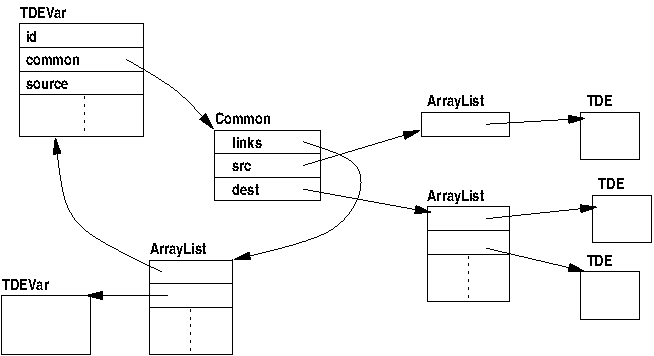
\includegraphics{TDEVar}




        \subsection{Common class}
        
            Every TDEVar contains a {\bf common} field. Where two TDEVar
            instances represent the same signal or signal array they can be
            merged by combining their common fields into a single shared
            object.
            
            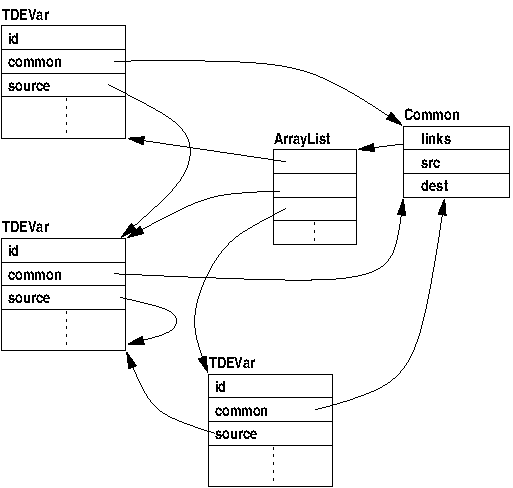
\includegraphics{TDEVarCommon}            
                      
            For example in the following 3PL code -
            
            \begin{lstlisting}[gobble=12, language=threepl]
                static(global.s1, "uint:4");
                static(global.s2, "uint:4");
                .
                .
                s1 <- s2;
                .
                .
            \end{lstlisting}
            
            The LHS reference in line 5 will generate a TDEVar which will appear
            in the TDE list as {\bf glob.s1.D[0..3]}, i.e. the D or data input
            to register s1. The RHS expression in line 5 will contain a TDEVar
            listed as {\bf glob.s2[0..3]}, the output of register s2.
            
            The assignment statement will connect the s1 data input to the
            s2 output, the s1 CE input (clock enable) to a control signal that goes high
            when the statement is executed and the s1 RES (reset) to GND.
            
            \begin{lstlisting}[gobble=12, language=tde]
            .
            .
            FMOD1/glob.s1.D[0..3] = FMOD1/glob.s2[0..3]
            FMOD1/glob.s1.CE[0..3] = S123
            FMOD1/glob.s1.RES[0..3] = GND
            .
            .
            REG
	            OUT  FMOD1/glob.s1[0..3]
	            <-
	            CLK  glob.c166
	            D    FMOD1/glob.s1.D[0..3]
	            CE   FMOD1/glob.s1.CE[0..3]
	            R    FMOD1/glob.s1.RES[0..3]
                {0x0}
            \end{lstlisting}
            
            After optimisation the CONNECT TDEs will be removed and the merged
            TDEVars will result in -
            
            \begin{lstlisting}[gobble=12, language=tde]
            .
            .
            REG
	            OUT  FMOD1/glob.s1[0..3]
	                        <-
	            CLK  glob.c166
	            D    FMOD1/glob.s2[0..3]
	            CE   s123
	            R    GND
                {0x0}
            \end{lstlisting}
            
            The funtionality has not changed and the merges are not logically
            necessary, but the TDE list is shorter and easier to read.

            The fields in common are -
            \blist
            \item   {\bf Clock clock\_var} \\
                    This is the clock variable for the clock domain of the
                    TDEVar(s). Constant TDEVars do not have a clock domain in
                    which case this is null.
            \item   {\bf ArrayList\verb'<'TDE\verb'>' dest} \\
                    A list of TDEs which are destinations (sinks) for this signal.
            \item   {\bf ArrayList\verb'<'TDE\verb'>' src} \\
                    A list of TDEs which are sources for this signal.
            \item   {\bf ArrayList\verb'<'TDEVar\verb'>' links} \\
                    TDEVars whose sources point here
            \blend

        
        \subsection{the merge method}
        
            As immediate execution proceeds connection of signals is done by
            method TDEList.connect(). This generates a {\bf CONNECT} TDE with one
            input TDEVar (the source) and one output TDEVar (the destination). If
            the input and output are different sizes then this represents a cast()
            which will pad or truncate the input array to match the output array.
            The input may even be a single signal to be connected to each bit of
            an output array, often the case with input GND or VCC.

            These CONNECT TDEs are resolved when processed by
            netlist.Xilinx.XTDECode(), however the presence of these CONNECT TDEs
            makes the intermediate netlist code difficult to read. As a dump of
            the intermediate netlist is a useful resource for checking the
            generated code for validity or determining problems with combinatorial
            expressions failing timing constraints, some effort has gone into
            resolving some of these {\bf CONNECT} TDEs during optimisation of the
            intermediate netlist, thus simplifying the presentation substantially.
            Note that this simplification is not required for generation of the
            final EDIF file from the intermediate netlist, it is simply to improve
            readability.

            The process is carried out during optimisation by examining all {\bf
            CONNECT} TDEs (there is a list of them in class TDEList) and where
            appropriate merging the set of destination TDEVars with the source
            TDEVar. This is done by method TDEVar.merge() using the common class.
        
            Method {\bf merge()} is called to merge two TDEVars. Before
            calling this method it must be determined that the two TDEVars
            meet one of the following criteria - 
            \blist
            \item  the TDEVars are for control signals (WordSpec is null).
            \item  the TDEVars are for clocks signals.
            \item  the TDEVars are for complete variables.
            \blend          
            This method does not perform these checks itself.
            
            The TDEVar to which merge() is applied should be the source and the
            argument to merge() should be a destination (sink). The source ID
            is used as the preferred ID.

            \begin{lstlisting}[gobble=8, language=java, xleftmargin=1cm]
            public void merge (TDEVar dtdev) {
                Common  dc = dtdev.common;   // destination common
                Common  sc = common;         // source common
                String  old_dest_id = dtdev.id;
                String  sid = id;

                sc.src.addAll(dc.src);                  // add source TDEs
                sc.dest.addAll(dc.dest);                // add destination TDEs
                sc.links.addAll(dc.links);              // link destination TDEVar links to the source of this TDEVar

                for (TDEVar t : dc.links) {
                    t.id = sid;
                    t.type = type;
                    t.wordspec = wordspec;
                    t.common = sc;
                    t.val = val;
                }

                // Update all occurrences of destination TDEVars with the same id
                // with the new source id.
                ArrayList<TDEVar>   al = catalog.get(old_dest_id);
                for (TDEVar tdev : al) {
                    if (tdev == dtdev)
                        continue;
                    tdev.id = sid;
                }
            }
            \end{lstlisting}

            Both the source TDEVar (this) and destination TDEVar (dtdev) may already
            have other TDEVars linked via their respective Commons as a result of
            previous merges. As a minimum every TDEVar has a link to itself in its
            Common.

            The destination common src, dest and links lists are appended to the
            corresponding lists in the source common.

            The source TDEVar will already have the same ID, type, WordSpec, Common
            class instance and val field in all linked TDEVars as result of previous
            merges. All linked destination TDEVars now have the source ID, type,
            WordSpec, Common and val field written into them. The merged destination
            TDEVar will now have the same ID, type, WordSpec, Common and val fields
            as the source TDEVar.

            Now that the destination TDEVars have had their IDs changed, any other
            instances of a TDEVar with the same ID, regardless of linkages or
            WordSpec, must be have their IDs changed as well. This is done using the
            catalog map.

            


        \subsection{target variables}

            Program target variables may be global, in which case the associated
            signal names begin with "glob.". Thus the output of a static global
            variable {\em a} would be a signal named {\em glob.a}.
            
            All other target variables are prefixed by a string constructed from all
            the hierachical scopes within which they are created. Each scope has an
            associated identifier which is either a module, procedure or function
            identifier or else a control structure indicator such as "if" or "when".
            Unique integers are appended to these identifiers to avoid duplication
            that might result from repeated entry to a scope. A target variable {\em
            b} created within a source file prog.3pl would have the identifier {\em
            prog.b}. If it was created after calling procedure proc then it would be
            {\em prog.proc\_1.b}. If the procedure were called again the resulting
            variable would be {\em prog.proc\_2.b}. A variable {\em c} created
            within a 'for' loop would have identifiers {\em prog.proc\_1.for\_1.c},
            {\em prog.proc\_1.for\_2.c} etc.
            
            Hierarchical signal names must include file paths of source files. To
            avoid very long identifiers file paths from {\bf source} or {\bf module}
            statements are replaced by arbitrary strings SRCn or FMODn in
            identifiers, {\bf n} being an integer. The optional intermediate code
            report file (prog.icl) lists these for reference purposes.

            Signal array references have a subscript range appended, even
            if the entire variable is accessed, e.g. "glob.a[0..7]". For
            multiple ranges comma-separated ranges are shown, e.g.
            "glob.a[0..7,16..23]"

            \subsubsection{static variables}

                A global static variable {\em s} of size 8 bits would have
                the following associated signal arrays -
                \blist
                \item   "glob.s[8]" - the data output signal array
                \item   "glob.s.D[8]" - the data input signal array
                \item   "glob.s.CE[8]" - the clock enable signal array
                \item   "glob.s.RES[8]" - the reset signal array
                \blend                
                The value of the variable is available via the data output
                signal. Assignments are made by driving the data input
                signal and asserting the clock enable signals to the selected
                bits. The reset signal array is used to return some
                portion of the variable to its initial state.

            \subsubsection{queue variables}

                A global queue variable {\em p} of size 8 bits would have
                the following associated signal arrays -
                \blist
                \item   "glob.p[8]" - the data output signal array
                \item   "glob.p.D[8]" - the data input signal array
                \item   "glob.p.NE" - output availability (not empty)
                \item   "glob.p.POP" - pop a datum
                \item   "glob.p.PUSH" - push a datum
                \item   "glob.p.NF" - input availability (not full)
                \item   "glob.p.CNT[4]" - buffer occupancy count
                \item   "glob.p.SPC[4]" - buffer space count
                \item   "glob.p.RSTAT[5]" - buffer status in read clock domain
                \item   "glob.p.WSTAT[5]" - buffer status in write clock domain
                \blend
                These signals are further described in the section on queue
                buffers below.

            \subsubsection{value variables}

                Value variables are effectively pointers and can be
                assigned multiple times. To ensure that each assigned
                value is distinguished a unique integer is appended.
                A global value variable {\em v} of 8 bits might thus appear
                variously as "glob.v\_1", "glob.v\_2" etc.                
                At the
                completion of immediate program execution the signal array
                "glob.v" would be equated with the last value the variable was
                assigned. This is an attempt to give the unappended variable
                identifier a sensible value during simulation.

            \subsubsection{priority variables}

                A global priority variable {\em p} of size 8 bits would have
                the following associated signal arrays -
                \blist
                \item   "glob.p[8]" - the data output signal array
                \item   "glob.p.D[8]" - the data input signal array
                \item   "glob.p.PE" - the 'else' signal
                \blend


            \subsubsection{memory variables}

                Memory variables have separate signal array identifiers
                for each port, e.g. global combinatorial-output memory
                {\em m} with two ports would have port output signal arrays
                "glob.m\_0" and "glob.m\_1".


        \subsection{expressions and execution control signals}

            The values resulting from expressions are given signal array
            identifiers of the form "E9".

            "startex" is a level signal which is asserted to begin
            execution. It is resynchronised to every clock domain, for example
            for a global clock {\em clk} the resynchronised start signal
            would be "glob.clk.start".

            Various other control signals are generated with prefices
            "A", "AND", "CD",, "CONST" "EO", "F", "FB", "FD", "FDCP", "FDRS",
            "FF", "FS", "I", "IN",, "INT" "INV", "LOG", "MADDR", "MDATA", "P",
            "PE", "PNTBUSY", "Q", "RADDR\_", "ROPAV", "S", "SAMPLEOUT", "SB",
            "SC", "SD", "SS", "start", "TF", "TS", "UINT" and "WADDR\_", integers
            being appended in each case to ensure identifiers are unique. there
            is no particular significance in these identifiers, the initial
            strings having been chosen to reflect the context in an attempt
            to improve readability of the intermediate code.




    \section{TDE class - CodeGen/TDE.java}

        The topological description is in terms of basic
hardware units such as registers, selectors,
control structures etc. linked by signals or signal
arrays.

The topological description class includes the following
fields -

{\bf type}

This indicates the type of element. Types are (see class
{\bf TDEConstants} -
\blist
\item   TDEType.SIG -       declare a signal or signal array
\item   TDEType.CONNECT -   connect a signal or signal array to another or to a
                            constant
\item   TDEType.SELECT -    select one of several inputs
\item   TDEType.TSELECT -   a 3-state driver
\item   TDEType.REG -       a register
\item   TDEType.WAIT -      wait for completion of parallel execution streams
\item   TDEType.DIVERGE -   handle queue divergence
\item   TDEType.INV -       invert a signal
\item   TDEType.AND -       AND 2 or more signals
\item   TDEType.OR -        OR 2 or more signals
\item   TDEType.XOR -       XOR 2 or more signals
\item   TDEType.OPERATOR -  apply an expression operator to operands
\item   TDEType.START -     start an execution stream
\item   TDEType.EXECP -     delay execution on queue availability
\item   TDEType.ILOOP -     control an infinite loop
\item   TDEType.DEL -       delay a signal one or more clock cycles
\item   TDEType.WHEN -      a 'when' statement
\item   TDEType.WHILE -     a 'while' statement
\item   TDEType.DOWHILE -   a 'do while' statement
\item   TDEType.PRIORITY -  a priority encoder
\item   TDEType.RESYNC -    resynchronise a pulse or edge to another clock
\item   TDEType.SAMPLE -    sample a value in another clock domain
\item   TDEType.QUEUEBUFFER - a queue variable (buffer)
\item   TDEType.IBUF -      an FPGA pad input buffer
\item   TDEType.OBUF -      an FPGA pad output buffer
\item   TDEType.DFF -       a D-type flip-flop
\item   TDEType.CRAM -      a combinatorial-output RAM
\item   TDEType.RRAM -      a registered-output RAM
\item   TDEType.CLOCK -     create a clock signal source
\item   TDEType.CLOCKINFO - a wrapper for information about a clock signal
\item   TDEType.ELEMENT -   create a specific FPGA vendor library element
\item   TDEType.PORT -      an external signal connection to/from another netlist
\item   TDEType.SPECIAL -   special functions for specific FPGA families
%            \item   TDEType.SIMREAD -   read a value for a variable from a file during simulation
%            \item   TDEType.SIMWRITE -  write a value from a variable to a file during simulation
%            \item   TDEType.SIMVAR -    communicate program variables to the simulator
\blend

{\bf ArrayList params} is a parameter section which includes such
things as initial values and flags. Items in the parameter
list may be type {\bf Integer}, {\bf String} or {\bf
Boolean}.

{\bf ArrayList inputs} and {\bf ArrayList outputs} are lists of 
TDEVars which are inputs and outputs to the TDE.

{\bf location}

This field gives the source file location.
Since these structures represent the hardware rather than the
source code the source file location does not provide a very
good cross reference to the source code. For example the
structure for a variable declaration includes all the logic
required to assign values to that variable, including input
selectors, however the selector logic is derived from the
various assignment statements which target that variable. The
line numbers of these statements are not available in the
variable structure. We could partition the logic into smaller
units to improve this situation, but that might impose
restrictions on the implementation and might also preclude some
simple low-level optimisations.

{\bf active}

This field indicates if the TDE is still in use.
During optimisation some TDEs are eliminated
and rather than delete them from the list of elements they
are instead tagged as inactive via this field.

{\bf no\_delete}

If this field is true the element should not be deleted. I
think the only use for this is for the SELECT TDE where
it is required when used for queue variable assignment that
a single input SELECT not be eliminated as redundant.

\subsection{constructors}

    There are a number of constructors all of which require the
    TDE type but which may omit parameter, input or output lists
    or source file location. Where omitted the lists are added
    later.

\subsection{methods}


    {\bf add2i()} \\ Add a signal to the input list.

    {\bf add2o()} \\ Add a signal to the output list.

    {\bf add2p()} \\ These add an item to the parameter list. There are multiple
    signatures for different argument types.

    {\bf addPin2Element()} \\ This method adds a pin and a connected signal to a
    TDE instance of type ELEMENT.

    {\bf addProperty2Element()} \\ This method adds a property to a TDE instance
    of type ELEMENT. The property name and value are added to the parameter list
    of the TDE instance.

    {\bf setElementPin()} This method adds a pin to a TDE instance of type
    ELEMENT. The port name, type (input, output, 3-state output or clock),
    associated TDEVar, port width and EDIF port array format are passed as
    arguments. The array size is used later (in XTDECode) to pad input nets
    formed from the TDEvar so that the full port width is connected even though
    the signal array may be narrower. Padding is GND unless the TDEVar is for a
    signed type in which case the MSB is propagated.


    {\bf redundant()} \\ This method examines a TDE to see if it contains
    redundancies or is entirely redundant. For example a duplicated selector
    data input is removed and the select input is ORed with the duplicate
    select. Logic gates with a single input are effectively removed (see below)
    and the single input is connected to the output directly.

    If the TDE is completely redundant it has all inputs, outputs and parameters
    removed, the active flag is made false and the method returns true. If the
    TDE is already in the TDE list it will be recognised as inactive during any
    traversals of the list and will be ignored.

    The method is called in only two places, TDEList.addTDE() and
    TDEList.optimise(). The first is called to add a TDE to the TDE list but
    does not do so if the TDE is wholly redundant (redeundant() returns true).
    The second is a TDE list optimiser which calls redundant() only for SELECT
    TDEs as a part of its optimisation of the list. Since the TDE is already in
    the list a true return from redundant() simply means the TDE has been made
    inactive and will be ignored when encountered again in any context.


    {\bf ncode()} \\ This method generates netlist code from the TDE. A switch
    on the TDE type selects a matching method in abstract class {\bf TDECode},
    these methods being overridden in class XTDECode in the case of Xilinx.

    {\bf deactivate()} \\ Make a TDE inactive by unlinking all inputs and
    outputs from the associated TDEVars (removing the reverse link), clearing
    the parameter list and setting boolean {\bf active} to false.

    {\bf removeInput()} \\ Remove a control signal input to a TDE. This is not
    used for signals which are arrays. The TDEVar is removed from the list of
    inputs and this TDE is removed from the destination list of the associated
    TYDEVar. This method assumes that there is only one occurrence of the TDEVar
    in the input list.

    {\bf replaceInput()} \\ Replace a TDEVar in the input list with another. The
    source link in the associated TDEVar is not changed by this method; it is
    assumed that that is done elsewhere.

    {\bf replaceOutput()} \\ Replace a TDEVar in the output list with another.
    The destination link in the associated TDEVar is not changed by this method;
    it is assumed that that is done elsewhere.
    
    {\bf dump()} \\ print a description of the TDE to the .icl file.


\subsection{signal linking}

    Input and output signals to a TDE are representad by class TDEVar.
    TDE fields {\bf input} and {\bf output} are lists of TDEVars (class
    {\bf TDEVarList} which extends class {\bf ArrayList}). The function of
    each input and output is dependant on the specific TDE type. A TDEVar
    in turn has a list of TDEs to which it is linked (within subclass Common).
    
    Optimisation of TDEs must handle this double linking where TDEVars are
    to be removed or relocated.
    

        

    \section{TDEVarList class - CodeGen/TDEVarList.java}

        The TDEVarList class extends class ArrayList. As well as providing a list
class for TDEVars it provides methods for generating Nets from TDEVars.

The TDEVar class does not implement proper netlist but just provides
a description of signals or signal arrays connected to TDEs. The TDEVar
identifiers and WordSpecs imply that 
WHen the complete TDE list is processed to generate the final netlist
each instance of a TDEVar must be converted to a Net. Methods in
TDEVarList do this conversion.

        

    \section{TDEList class - CodeGen/TDEList.java}

        This class extends ArrayList. A TDE list is the intermediate form of generated
code. The list has variable declarations at the front followed by logic using
those variables. An index, 'variables', is used to maintain the insertion point
for variables at the head of the list. Method addTDE() appends code TDEs to the
tail of the list. Method addVTDE inserts TDEs at the end of the leading variable
section of the list. Field 'index' provides a unique integer to append to the
end of generated signal names. It is incremented after each use.

There are a number of additional static lists of particular TDEs that are used
for optimisation. These are -

\blist
\item connects - CONNECT TDE
\item dels - DEL TDE
\item regs - REG TDE
\item ops - OPERATOR TDE
\item whens - WHEN TDE
\item iloops - ILOOP TDE
\item waits - WAIT TDE
\item gates - AND, OR, XOR TDE
\item sels - SELECT TDE
\item execps - EXECP TDE
\item dffs - DFF TDE
\blend

These lists avoid the need to scan the entire TDE list when optimising
particular TDE types.

Another static list, {\bf branches}, contains details of branch statements for
later optimisation.

The static list {\bf start\_dffs} is built up as ILOOPs are optimised. It is
later scanned to eliminate duplicate DFF elements with common start signal.

{\bf static  HashMap\verb'<'String,TDE\verb'>' uelements} is a map of
elements created using the ELEMENT TDE. Static {\bf current\_uelement} is
the most recent ELEMENT TDE to which connections can be added without
explicitly using the element identifier.



\subsection{method optimise}

    This method is called from the Main method (ThreePL.jj) after
    immediate execution. Optimisation, including that done in this
    method, is described in a later chapter.

\subsection{method ncode}

    This method generates the EDIF netlist. It does this in the following
    steps -
    
    The TDE list is traversed (skipping the initial signal declaration
    section) calling TDE.ncode() on each to generate netlist elements and nets
    via XTDECode methods.
    
    \begin{lstlisting}[gobble=8, language=java]
        Iterator<TDE>   it   = iterator();
        TDE             tde  = null;
        while (it.hasNext()) {
        tde = it.next();
        if (tde.isActive())
            tde.ncode(family);
        }
    \end{lstlisting}
    
    A list of external ports is built from data previously extracted
    when processing IBUF and OBUF TDEs in XTDECode.

    \begin{lstlisting}[gobble=8, language=java]
        family.makePorts();
    \end{lstlisting}
    
    Any flip-flops in output pads whose outputs are used internally as well are
    duplicated by a CLB flip-flop (XNetListOptimise.optimiseOBUF() and
    XNetListOptimise.optimiseOBUFT()). Gates with output not connected, gates
    with one input and gates with duplicated inputs are removed or modified as
    appropriate. Family-specific devices such as XORCY, MUXF etc. are similarly
    optimised.
     
    \begin{lstlisting}[gobble=8, language=java]
        passes = family.optimiseNetlist();
    \end{lstlisting}

    Generic elements are converted to family-specific ones where necessary.
    Up to this point gates are as wide as required by the context. Here they are
    converted to combinatorial logic matching the CLBs in the FPGA family.
        
    \begin{lstlisting}[gobble=8, language=java]
        family.convertGenericToSpecific();
    \end{lstlisting}

    The netlist file header is written out.
    
    The netlist cells are then written out to the netlist file.
    
    \begin{lstlisting}[gobble=8, language=java]
        Element.outputCells(pw, view);
    \end{lstlisting}

    The list of external ports is now written to the netlist file.
    
    \begin{lstlisting}[gobble=8, language=java]
        TDECode.outputExterns(pw);
    \end{lstlisting}

    Element instances are written.
   
    \begin{lstlisting}[gobble=8, language=java]
        Element.outputInstances(pw, view);
    \end{lstlisting}

    The nets are now written.
    
    \begin{lstlisting}[gobble=8, language=java]
        Net.outputInstances(pw);
    \end{lstlisting}

    The netlist file is now completed by writing out the part specification
    and the final curly bracket.
    
    Finally constraints are written to the .ncf (ISE) or .xdc (Vivado) file.

    \begin{lstlisting}[gobble=8, language=java]
        family.outputConstraints(author, netlistcomments);
    \end{lstlisting}





    \section{Intermediate code optimisation}
    
        The intermediate code is optimised prior to conversion to
        a netlist structure. The optimisation is described in a later chapter.

    \section{Conversion of intermediate code to netlist structure}

        The intermediate code consists largely of elements which can be
        expected to be available in any FPGA. This set of elements is enough
        to implement any 3PL program. Signals and signal arrays are arguments
        to these elements.

        The intermediate code elements are -
        \blist
        \item   AND -       AND 2 or more signals
        \item   CONNECT -   connect a signal or signal array to another or to a
                            constant
        \item   CRAM -      a combinatorial-output RAM
        \item   DEL -       delay a signal one or more clock cycles
        \item   DFF -       a D-type flip-flop
        \item   DIVERGE -   handle queue divergence
        \item   DOWHILE -   a 'do while' statement
        \item   ELEMENT -   create a specific FPGA vendor library element
        \item   EXECP -     delay execution on queue availability
        \item   IBUF -      an FPGA pad input buffer
        \item   ILOOP -     control an infinite loop
        \item   INV -       invert a signal
        \item   OBUF -      an FPGA pad output buffer
        \item   OPERATOR -  apply an expression operator to operands
        \item   OR -        OR 2 or more signals
        \item   PORT -      an external signal connection to/from another netlist
        \item   PRIORITY -  a priority encoder
        \item   QUEUEBUFFER - a queue variable (buffer)
        \item   REG -       a register
        \item   RESYNC -    resynchronise a pulse or edge to another clock
        \item   RRAM -      a registered-output RAM
        \item   SAMPLE -    sample a value in another clock domain
        \item   SELECT -    select one of several inputs
        \item   SIG -       declare a signal or signal array
%        \item   SIMREAD -   read a value for a variable from a file during simulation
%        \item   SIMWRITE -  write a value from a variable to a file during simulation
%        \item   SIMVAR -    communicate program variables to the simulator
        \item   SPECIAL -   special functions for specific FPGA families
        \item   START -     start an execution stream
        \item   TSELECT -   a 3-state driver
        \item   WAIT -      wait for completion of parallel execution streams
        \item   WHEN -      a 'when' statement
        \item   WHILE -     a 'while' statement
        \item   XOR -       XOR 2 or more signals
        \blend


        \section{Intermediate code elements}



            \subsection{AND}

                \subsubsection{purpose}

                    An AND gate for control signals.

                \subsubsection{arguments}

                    \begin{tabular}{| l | l |}
                    \hline
                    Parameters  & none \\
                    \hline
                    Inputs      & input signal \\
                                & input signal \\
                                & . \\
                                & . \\
                    \hline
                    Outputs     & AND signal \\
                    \hline
                    \end{tabular}

                \subsubsection{description}

                    AND two or more input signals, the result appearing on the
                    output.

                \subsubsection{dump format}

                    \begin{lstlisting}[gobble=20, language=tde]
                        S11 = A12 & A14 & S8
                    \end{lstlisting}

                \subsubsection{logic description}

                    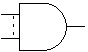
\includegraphics{and}

                    Xilinx implementation -

                    AND gates with 1 to 4 inputs will be implemented in a
                    single LUT (single input gates will be eliminated during
                    low-level code generation). AND gates with more than 4 inputs
                    use the carry chain to AND together the outputs of 1 to 4
                    input LUT AND gates.


        \subsection{CONNECT}

            \subsubsection{purpose}
            
                Connect signals or signal arrays.

            \subsubsection{arguments}
            
                \begin{tabular}{| l | l |}
                \hline
                Parameters  & optional boolean for sign extension \\
                            & optional long right shift count \\
                            & optional boolean for left justification \\
                \hline
                Inputs      & signal, signal array or constant \\
                \hline
                Outputs     & signal or signal array \\
                \hline
                \end{tabular}

            \subsubsection{description}
            
                This connects signals or signal arrays.
                
                If there is a single
                boolean parameter, a true value indicates sign extension will be
                used if the output is wider than the input. A false value or
                missing parameter indicates zero padding will be used if the
                output is wider than the input. If the output is narrower than
                the input then truncation will occur and the parameter is not
                relevant. The parameter may be omitted or null.
                
                If there is a second parameter it is a right shift count. The 
                sign extension indicated by the first parameter is observed.
                If the first parameter is present and true then the sign bit will
                be propagated during the right shift.
                The parameter may be omitted or null.
                
                If there is a third parameter it indicates that the input
                is to be left justified with respect to the output, i.e.
                input bits wil be connected in order from MSB to LSB. There
                is no recognition of a sign bit. Where
                a size mismatch occurs truncation or zero padding will be used
                at the LSB end. The parameter may be omitted or null.

                If there are no parameters then signal connection occurs in the
                following scenarios -
                \blist
                \item   signal = signal
                \item   signal array = signal array
                \item   signal array = signal
                \item   signal array = constant
                \blend
                The first two cases connect signals or signal arrays together.
                The input (RHS) should be a source and the output (LHS) a sink.
                Signal arrays must be the same size, but the third case is
                allowed - a signal array connected to a single signal source
                (often GND or VCC).

                In the last case a signal array is connected to a pattern of GND
                and VCC to implement a 64-bit constant. The constant (which may
                be signed) will be truncated to fit the signal array. This case
                may include a sign extension parameter, but the parameter is not
                relevant since the constant is guaranteed to fit the output
                width, including the sign.

            \subsubsection{dump format}
            
                \begin{lstlisting}{gobble=16, language={tde}}
                       S11 = TS15
                       E1[0..7] = glob.a[8..15]
                       E2[0..2] = VCC
                       E3[0..7] = 17
                       E4[0..15] = glob.v[0..11] cast - pad
                       E5[0..15] = glob.v[0..11] cast - sign_extend
                \end{lstlisting}


            \subsubsection{logic description}

                No logic is generated by this element.


            \subsection{CRAM}

                \subsubsection{purpose}

                    Combinatorial-output RAM.

                \subsubsection{arguments}

                    \begin{tabular}{| l | l |}
                    \hline
                    Parameters  & Integer number of ports \\
                                & Integer data width in bits \\
                                & Integer address width in bits \\
                                & String[] optional initialisation \\
                                & String - "timingname" attribute key \\
                                & String - data for "timingname" attribute \\
                    \hline
                    Inputs      & clock signal, port0 \\
                                & address array, port0 \\
                                & data\_in array, or null, port0 \\
                                & write signal, or null, port0 \\
                                & clock signal, port1 \\
                                & address array, port1 \\
                                & data\_in array, or null, port1 \\
                                & write signal, or null, port1 \\
                                & ..etc.. \\
                    \hline
                    Outputs     & data\_out array, or null, port0 \\
                                & data\_out array, or null, port1 \\
                    \hline
                    \end{tabular}

                \subsubsection{description}

                    This is a RAM with a clocked write but a combinatorial read.
                    At all times the output for a port reflects the memory
                    contents at the location indicated by the current address
                    input.

                    The 2nd parameter gives the data width and the address width
                    gives the memory depth (number of words). All port addresses
                    must be the same width and all port data inputs and outputs
                    must be the same width.

                    The initialisation string array has one entry for each
                    initial value. Each entry is a hexadecimal string. The
                    initialisation array may be smaller than the depth of the
                    RAM but not larger. The initialisation parameter may be
                    omitted in which case the RAM is explicitly initialised to
                    all 0. Initialisation data is written to the NCF file.
                    
                    If a timing name is supplied a TNM entry is added to the
                    NCF file.

                    Ports which are not written have null arguments for the data
                    in and the write enable. Ports which are not read have null
                    arguments for the data out.

                    For Xilinx FPGAs Combinatorial-output RAM is CLB RAM. The
                    address width is limited to a maximum of 9 bits (a depth of 512
                    words). The data width is not limited.
                    
                    There is one optional attribute which is a timing group name.

                \subsubsection{dump format}

                    \begin{lstlisting}[gobble=20, language=tde]
                        CRAM - 2 ports
                            OUT  null
                            OUT  SAMPLEOUT168[0]
                            <-
                            CLK  glob.c100
                            ADDR WADDR_160[0..1]
                            DATA glob.frontend_0.sdc_in_0.reset_1[0]
                            WE   VCC
                            CLK  null
                            ADDR RADDR_161[0..1]
                        initialised{timingname=cram1}
                    \end{lstlisting}

                    The presence of an initialisation argument is flagged
                    but the values are not listed.

                \subsubsection{logic description}

                    For Xilinx combinatorial output RAM is CLB RAM. If two
                    ports are used the second port is read-only. Single
                    port CLB RAM has an address width of 5 and dual port
                    CLB RAM an address width of 4. In both cases the data
                    width is 1. For greater address widths CLB RAMs are
                    multiplexed, for example a dual port 64 deep RAM -
                    
                    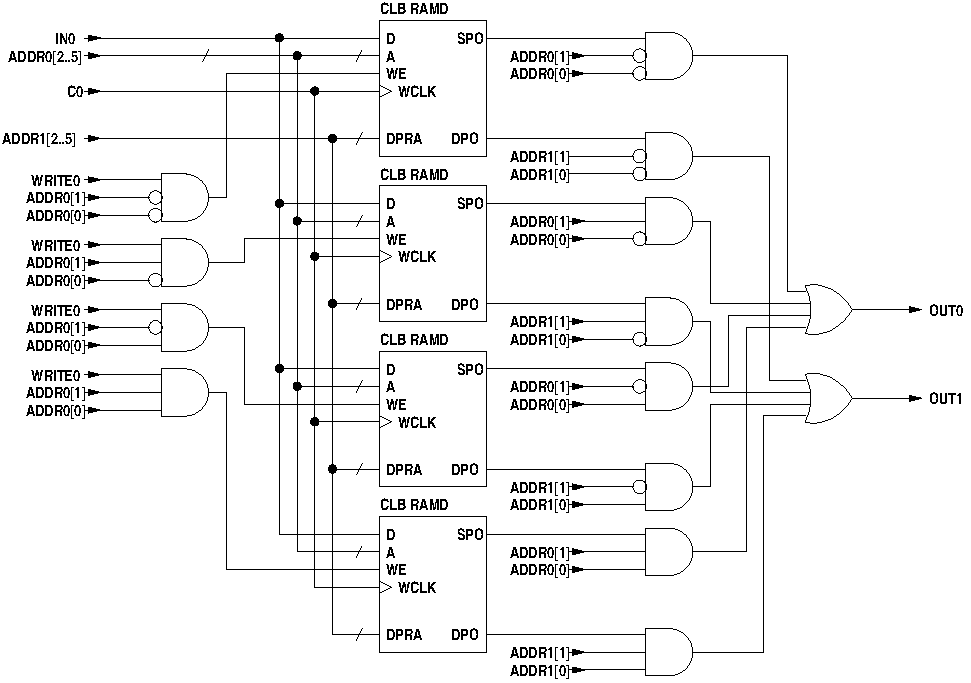
\includegraphics{cram}
                    
                    This is only one data bit wide and is repeated for each
                    additional data bit with the other signals in parallel.


            \subsection{DEL}

                \subsubsection{purpose}

                    To create a delay line to delay a signal one or more clock
                    cycles. The delay may be
                    variable.

                \subsubsection{arguments}

                    \begin{tabular}{| l | l |}
                    \hline
                    Parameters  & Integer number of clock cycles to delay if constant,
                                  else 0 \\
                                & String array  initial words in line as array of hexadecimal strings \\
                    \hline
                    Inputs:     & clock signal \\
                                & input signal array \\
                                & delay signal array  number of clock cycles to delay if
                                  variable, else null \\
                                & enable signal delay steps if high - null for
                                  every cycle \\
                                & reset or null \\
                    \hline
                    Outputs     & output signal \\
                    \hline
                    \end{tabular}

                \subsubsection{description}

                The input signal appears at the output one or more clock cycles
                later. The reset signal returns the logic to its initial
                state. It may be omitted or null.
                
                If the reset is present then a fixed delay line will be created
                using flip-flops, in which case the variable length input must
                be null.
                
                If the variable length input is not null the delay line will
                use CLB shift registers and the reset input must be null.
                The delay length is limited to 16 or 32 depending on the
                FPGA.
            
                If the variable delay is used, this value selects the point
                in the delay line from which the output is taken. 0 selects
                the output of the 1st delay element and 15 the output of the
                16th delay element. Note that changing this value will result
                in data being skipped (decreasing) or repeated (increasing).

                If there is initialisation data the number of words will
                be equal to the delay line length.
                If there is no initialisation data these parameters will
                be omitted.

                \subsubsection{dump format}

                    \begin{lstlisting}[gobble=20, language=tde]
                        DEL E69[0..3] <- p.in[0..3] CLK glob.c166 delay 18 initialised
                    \end{lstlisting}

                \subsubsection{logic description}

                    Xilinx implementation -

                    This element is implemented sharing the code for
                    SPECIAL element (code 4) which provides a general delay
                    line using Xilinx CLB shift registers.

                    A delay of three or fewer cycle is implemented using
                    flip-flops. Delays of more than three cycles may use one or
                    more CLB shift registers. If a reset signal is present
                    flip-flops must be used, the reset signal being connected to
                    the reset inputs of the flip-flops.


            \subsection{DFF}

                \subsubsection{purpose}

                    A D-type flip-flop.

                \subsubsection{arguments}

                    \begin{tabular}{| l | l |}
                    \hline
                    Parameters  & Boolean optional initial value \\
                                & Boolean false or omitted if set and reset are synchronous
                                  , true if asynchronous \\
                                & String  optional timing group identifier \\
                                & String  optional constraint \\
                                & String  ... etc \\
                    \hline
                    Inputs      & data\_in signal, or null \\
                                & clock signal, or null \\
                                & clock enable signal, or null \\
                                & reset/clear signal, or null \\
                                & set/preset signal, or null \\
                    \hline
                    Outputs     & data\_out signal \\
                    \hline
                    \end{tabular}

                    A number of constraint strings may appear at the end of the
                    parameter section. These strings will be applied to the FD
                    prepended with "INST name " where 'name' is the generated
                    netlist identifier for the FD.
                    

                \subsubsection{description}

                    This provides a basic D-type flip-flop. Unused arguments may be
                    null and unused trailing arguments may be omitted.

                \subsubsection{dump format}

                    \begin{lstlisting}[gobble=20, language=tde]
                        DFF FDRS164 <- D=INV163, C=glob.sdclk0
                    \end{lstlisting}


            \subsection{DIVERGE}

                \subsubsection{purpose}

                    A controller for divergent queue signals. Where a queue is read
                    within more than one module it is required that each module
                    execute a read before the datum is popped. Until all destination
                    modules have executed a read the queue must appear unavailable
                    for reading to those modules that have already executed a read.
                    This is accomplished by inserting this DIVERGE element between
                    the queue .NE and .POP signals and the .NE and .POp signals
                    seen by the queue reads in each destination module.

                \subsubsection{arguments}

                    \begin{tabular}{| l | l |}
                    \hline
                    Parameters  & none \\
                    \hline
                    Inputs      & clock signal \\
                                & reset signal \\
                                & queue not empty signal \\
                                & module queue pop signal \\
                                & module queue pop signal \\
                                & . \\
                                & . \\
                                & . \\
                    \hline
                    Outputs     & queue pop signal \\
                                & module queue not empty signal \\
                                & module queue not empty signal \\
                                & . \\
                                & . \\
                                & . \\
                    \hline
                    \end{tabular}

                \subsubsection{description}

                    This splits the source queue .NE (read availability) and
                    .POP (acknowledge) signals into a pair per destination
                    module.

                    The 1st input is the output (read) clock signal for the
                    queue.

                    The 2nd input is an optional reset signal to clear this
                    element to initial status. This occurs if the associated
                    QUEUEBUFFER is reset.

                    The 3rd input is the .NE (read availability) signal from the
                    queue.

                    The 4th and following inputs are the .POP signal from the
                    destination modules.

                    The 1st output signal is the .POP (acknowledge) signal to
                    the queue.               

                    The 2nd and following outputs are the .NE signals to the
                    destination modules. If there is only one destination module
                    the .NE and .POP signals should be just connected through.
                    If all destination acknowledge signals go high
                    simultaneously the acknowledge signal to the source also
                    goes high, otherwise it goes high when the last destination
                    acknowledge signal goes high. The destination acknowledge
                    signal is high for one clock cycle. When each destination
                    acknowledge signal goes high the matching destination
                    availability signal will go low at the next clock cycle
                    unless all destination modules have also acknowledged in
                    which case destination availability signals will be the be
                    the same as the source availability signal.


                \subsubsection{dump format}

                    \begin{lstlisting}[gobble=20, language=tde]
                        DIVERGE {
                            glob.p.POP
                            S15
                            <-
                            c100
                            S11
                            glob.p.NE
                        }
                    \end{lstlisting}

                \subsubsection{logic description}

                    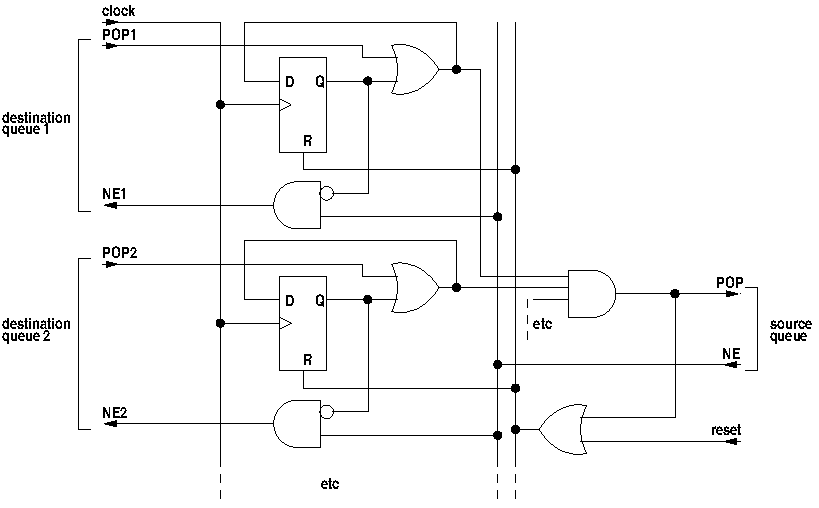
\includegraphics{diverge}


            \subsection{DOWHILE}

                \subsubsection{purpose}

                    A {\em do while} statement.

                \subsubsection{arguments}

                    \begin{tabular}{| l | l |}
                    \hline
                    Parameters  & none \\
                    \hline
                    Inputs      & start signal \\
                                & test signal \\
                                & block finish delayed signal \\
                                & clock signal \\
                                & optional reset signal or null \\
                    \hline
                    Outputs     & start signal for the body \\
                                & DO WHILE finish signal \\
                    \hline
                    \end{tabular}

                \subsubsection{description}

                    The start input signal starts the first iteration of the loop
                    by propagating straight through to the body start output
                    signal. The block finish delayed input signal comes from the
                    block finish signal, possibly via an EXECP if the test signal
                    comes from an expression containing queue reads. The block
                    finish delayed input signal is then routed either through to
                    the body start output signal (test succeeds) or via a one cycle
                    delay to the finish output signal (test fails).

                \subsubsection{dump format}

                    \begin{lstlisting}[gobble=20, language=tde]
                        DO WHILE {
                            START_B     S23
                            FINISH      F35
                            <-
                            START       S24
                            TEST        E31[0]
                            CONTIN      F33
                            C           glob.c100
                            RESET       s34
                        }
                    \end{lstlisting}

                \subsubsection{logic description}

                    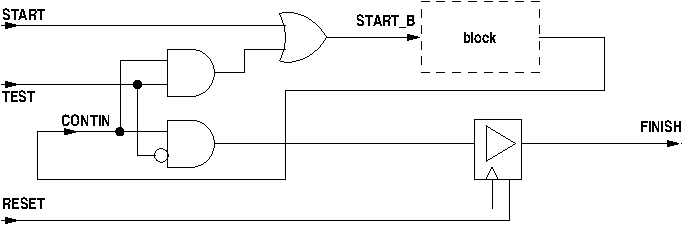
\includegraphics{dowhilea}

                    The START signal is passed straight through to the block
                    execution signal output START\_B. The block finish signal
                    FINISH\_B loops back via conditional logic where the test
                    expression is sampled. If the test succeeds FINISH\_B is passed
                    throught to START\_B to begin the next iteration otherwise it
                    is passed to FINISH via a DEL. A RESET clears the DEL. The DEL
                    is required to avoid a race condition through to the following
                    statement.

                    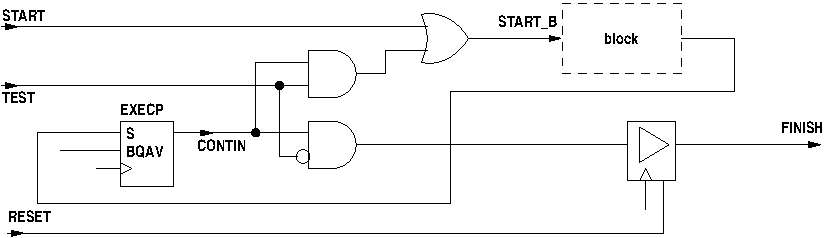
\includegraphics{dowhileb}

                    An EXECP is required if the test expression contains queue
                    reads. The EXECP controls the FINISH\_B signal prior to the
                    conditional logic. A RESET clears the DEL and EXECPs. The DEL
                    is required to avoid a race condition through to the following
                    statement.


        \subsection{ELEMENT}

            \subsubsection{purpose}
            
                Create an instance of a netlist element.
                
            \subsubsection{arguments}
            
                \begin{tabular}{| l | l |}
                \hline
                Parameters  & String  the element name               \\
                            & String  netlist block name or null     \\
                            & String    port name         | 1st port \\
                            & integer   port type         |          \\
                            & integer   port width        |          \\
                            & integer   port array format |          \\
                            .                             | 2nd port \\
                            .                                        \\
                \hline
                Inputs      & input 1                                \\
                Inputs      & input 2                                \\
                .                                                    \\
                .                                                    \\
                \hline
                Outputs     & output 1                               \\
                Outputs     & output 2                               \\
                .                                                    \\
                .                                                    \\
                \hline
                \end{tabular}

            \subsubsection{description}

                This is used to explicitly create a component element. It can be
                used to access library components which are not created
                implicitly by other TDEs. A TDE of this type can also be
                created from 3PL source code using inbuilt procedures
                {\bf element()} and {\bf elementconnect()}. This allows
                fpag-specific elements to be created by 3PL library code
                rather than being built into 3PL.

                The first parameter is the element name. The optional second
                parameter is a netlist identifier for this instance of the
                element. If null an arbitrary identifier of the form "b123" will
                be generated.
                
                The following parameters are quadruples giving the port name,
                port type (0 input, 1 output, 2 3-state output, 4 clock input),
                port width in bits and port array format, 0 for non-array
                ports, 1 for pins as A1, A2, A3 etc. and 2 for EDIF pin arrays.
                For each quadruple there will be an associated signal in the
                input or output list in the order of occurrence in the
                parameter list.
            
            \subsubsection{dump format}
            
                \begin{lstlisting}{gobble=16, language={tde}}
                    ELEMENT DCM block dcm1
	                    PIN CLKIN I glob.ruclk
	                    PIN CLKFB I prog.cfb
	                    PIN CLK0  O prog.cfb_raw
	                    PIN CLKDV O prog.pclk_raw
                \end{lstlisting}


            \subsection{EXECP}

                \subsubsection{purpose}

                    An execution wait for queue availability and/or priority
                    grant.

                \subsubsection{arguments}

                    \begin{tabular}{| l | l |}
                    \hline
                    Parameters  & none \\
                    \hline
                    Inputs      & clock signal \\
                                & start signal \\
                                & buffered queue availability signal \\
                                & unbuffered queue write availability signal \\
                                & unbuffered queue read availability signal \\
                                & priority output signal or null \\
                                & reset or null \\
                    \hline
                    Outputs     & delayed start signal \\
                                & priority input signal or null \\
                                & execution write pending signal or null \\
                                & execution read pending signal or null \\
                    \hline
                    \end{tabular}
                    
                    If the wait is for queue availability alone the
                    priority input and output arguments are null. If the
                    wait is for priority alone the queue availability arguments
                    is null. The reset argument is null if there is no
                    reset signal.

                \subsubsection{description}

                    This element delays an execution signal if it is necessary to
                    wait for queue availability, for priority or both. The buffered
                    queue availability input is high if all associated buffered
                    queues to be read or written are available. The unbuffered queue
                    availability inputs are similar but the write and read
                    availabilities are on separate inputs.

                    If the queue availability inputs are high and the priority
                    encoder passes the signal, the execution signal is passed
                    through without delay. If the queue availability inputs are not
                    all high or priority has been pre-empted, the execution signal
                    is stored until the queue availabilities are high and priority
                    is granted at which time a single cycle output pulse is
                    generated. An input execution signal must not occur when an
                    output is pending however it may occur on the cycle following
                    the output pulse. The queue availability inputs may be several
                    queue availabilities ANDed together. The reset input, if not
                    null, is used to clear any pending execution (waiting on queue
                    availability or priority). The pending signals are used to
                    notify unbuffered queues that a write or read is pending
                    awaiting unbuffered queue availability. It is asserted when the
                    start signal is asserted or the registered start signal is
                    asserted and all buffered queues are available. The output need
                    not have an argument (null) if unbuffered queues are not
                    involved.

                \subsubsection{dump format}
                    
                    The dump format depends on whether the EXECP has priority
                    inputs/outputs or unbuffered queues.
                    
                    For normal buffered queues -
                    \begin{lstlisting}[gobble=20, language=tde]
                        EXECP no priority, buffered queues only {
	                        START_DEL SD423
	                        <-
	                        CLK       glob.c32
	                        START_IN  F392
	                        BQAV      tx.NE
                        }
                    \end{lstlisting}

                    With both buffered and unbuffered queues -
                    \begin{lstlisting}[gobble=20, language=tde]
                        EXECP no priority, unbuffered (+ buffered) queues {
	                        START_DEL SD23
	                        WPENDING   WP18
	                        RPENDING   RP17
	                        <-
	                        CLK       glob.c32
	                        START_IN  S13
	                        BQAV      VCC
	                        UBQWAV    VCC
	                        UBQRAV    prog.ubq1.NE
                        }
                    \end{lstlisting}
                    
                    Buffered queues with priority -
                    \begin{lstlisting}[gobble=20, language=tde]
                        EXECP priority, buffered queues only {
	                        START_DEL SD9750
	                        PRI_IN    WPIN9742[0]
	                        <-
	                        CLK       glob.pclk
	                        START_IN  TS9737
	                        BQAV      kandinski.processing_0.mark.NF
	                        PRI_OUT   kandinski.processing_0.marker_0.pri[1]
                    \end{lstlisting}

                \subsubsection{logic description}

                    If there are no priority signals the delayed start output
                    depends only on the start and buffered queue availability
                    input signals -
                    
                    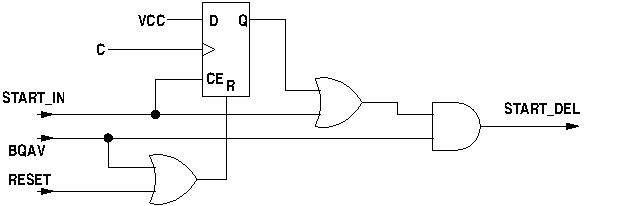
\includegraphics{execp1}

                    BQAV is the AND of the read or write availability signals of
                    all buffered queues upon which this EXECP execution depends.
                    If BQAV is high START\_IN is gated straight through to
                    START\_DEL and the flip-flop doesn't change, being held
                    reset by BQAV. If BQAV is low when START\_IN arrives
                    the flip-flop is set and START\_DEL remains low. When BQAV
                    subsequently goes high START\_DEL goes high because the
                    flip-flop is set. On the next clock edge the flip-flop is
                    reset and START\_DEL goes low again.
                    
                    If there are priority input and output signals but no
                    availability signal -
                    
                    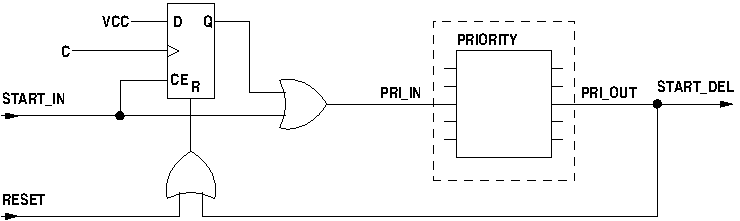
\includegraphics{execp2}
                    
                    The delayed start now requires the priority encoder
                    to pass the start, otherwise it is latched. The flip-flop
                    is cleared when the delayed start finally occurs. The
                    flip-flop will not latch the start signal if the priority
                    encoder passes the signal.
                    
                    The priority encoder is required for {\bf waitpri} and {\bf
                    waitprilock} statements. The priority encoder (priority mode
                    variable) is shown above in a dashed rectangle as it exists
                    outside the EXECP block, the input and output signals for a
                    particular priority level being passed as arguments to the
                    EXECP. The highest priority input, 0, is reserved, array
                    members 1 and above being used for statement priority.
                    Priority input 0 is used to lock out all other priority
                    requests when {\bf waitprilock} is used and is asserted by a
                    flip-flop which is set by any executing waitprilock
                    instances and cleared later by a {\bf priunlock} statement.
                    
                    If both priority and buffered queue availability signals are present -
                    
                    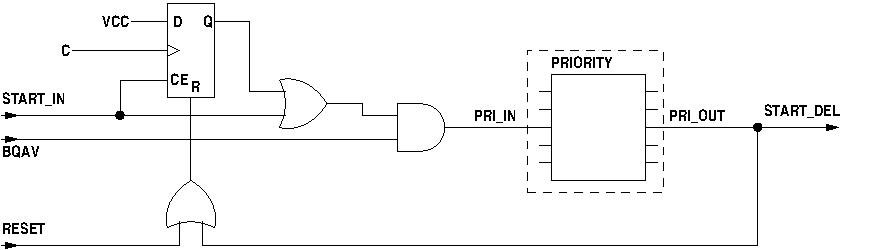
\includegraphics{execp3}
                    
                    The delayed start now requires the priority encoder to
                    pass the signal and the availability signal to be asserted.
                    If this is true when the start signal is asserted the
                    flip-flop will not be set as its reset will also be
                    asserted.
                    
                    Note that in the case where more than one waitpri
                    uses the same priority level the START\_DEL signal for
                    each must be the AND of PRI\_IN and PRI\_OUT instead
                    of just PRI\_OUT, otherwise the START\_DEL signals
                    for the separate occurences would be connected! The
                    multiple PRI\_IN signals to the priority variables
                    will be ORed.
                    
                    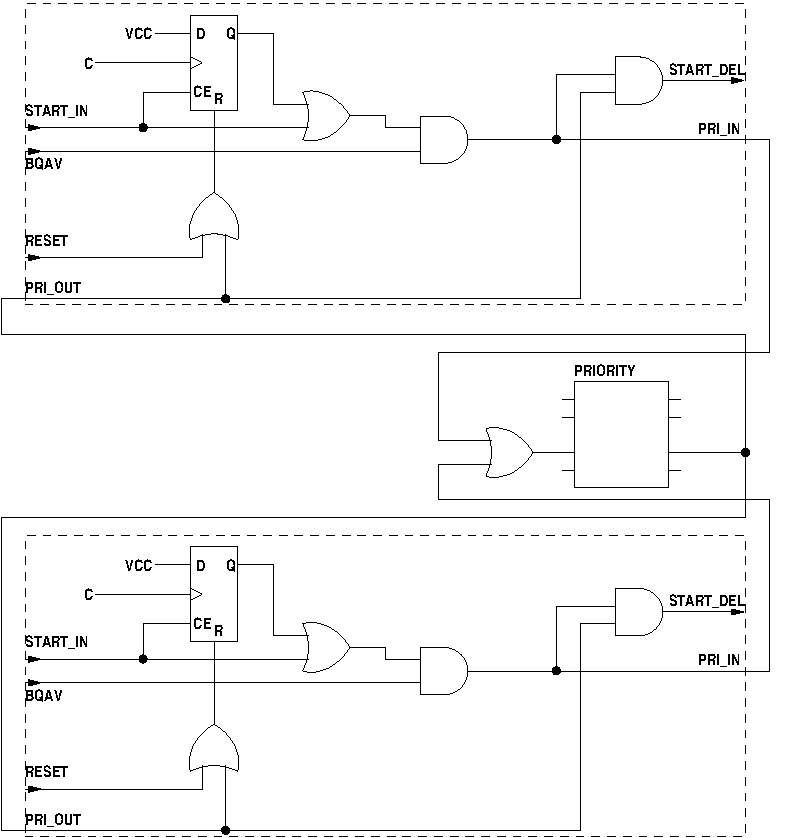
\includegraphics{execp4}
                    
                    Multiple use of the same priority level is determined by
                    calling the isMultiple() method in class exec/Priority.java
                    with the aray index as parameter. The Priority class instance
                    and the index are found from the 4th input argument TDEVar.
                    
                    If unbuffered queue availability signals are present -
                    
                    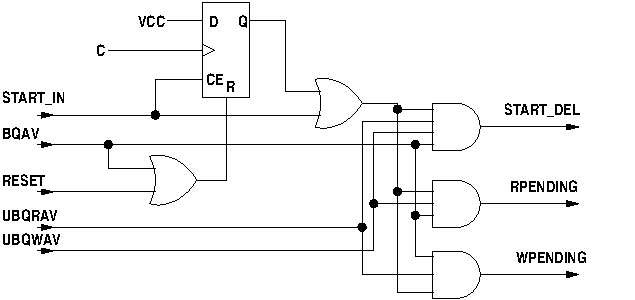
\includegraphics{execp5}
                    
                    BQAV, UBQRAV and UBQWAV are the ANDed availability signals for
                    buffered queues, unbuffered queues being read and unbuffered
                    queues being written respectively. Where any of these three have
                    no queues associated with the EXECP the availability signal is
                    null and the input to the EXECP will be VCC.

                    The delayed start now depends additionally on the unbuffered
                    queues being available plus any buffered queues being available.
                    When a start has been received and the buffered queue
                    availability signal is high RPENDING is asserted if UBQAV is
                    high and WPENDING is asserted if UBQWAV is high. These
                    cross-dependencies for a chain of dependencies through related
                    unbuffered queue assignments - see (\ref{ubqueuerw}).

                    When all associated unbuffered queues are available START\_DEL
                    will be asserted in both the writing and reading EXECPs so that
                    both threads can proceed. Since the QUEUEBUFFER simply has the
                    data input connected to the output the written data will be
                    transferred directly from writers to readers.
                    


            \subsection{IBUF}

                \subsubsection{purpose}

                    A buffered external input signal.

                \subsubsection{arguments}

                    \begin{tabular}{| l | l |}
                    \hline
                    Parameters  & String  - optional element identifier \\
                                & String  - input package pin \\
                                & String  - optional input package pin for differential input\\
                                & Boolean - ibufg flag \\
                                & Boolean - differential flag \\
                    \hline
                    Inputs      & input signal from pad \\
                                & optional differential input signal from pad or null \\
                    \hline
                    Outputs     & output signal \\
                                & optional differential output signal or null \\
                    \hline
                    \end{tabular}

                \subsubsection{description}

                    This buffers an external input signal. The first parameter
                    specifies the ID given to the IBUF element. The second
                    parameter gives the primary FPGA pad designation. The third
                    parameter is an optional second input pad for differential
                    input or null. The fourth parameter is true for an IBUFG or
                    IBUFGDS The last parameter is true if the input is
                    differential (IBUFDS, IBUFGDS, IBUFDS\_DIFF\_OUT).

                    There is a primary input signal followed by a second input
                    signal if there is differential input to the IBUF (IBUFDS,
                    IBUFGDS, IBUFDS\_DIFF\_OUT) or null (IBUF, IBUFG).

                    There is a primary output signal followed by a second output
                    signal if there is differential output from the IBUF
                    (IBUFDS\_DIFF\_OUT) or null (IBUF, IBUFG, IBUFDS, IBUFGDS).

                    There must be a {\bf loc} entry to specify the package pin.
                    For differential inputs two consecutive pins are used,
                    positive input followed by negative input.
 
                \subsubsection{dump format}

                    \begin{lstlisting}[gobble=20, language=tde]
                        IBUF    INPUT327[0] <- PORT_P88 loc=P88, IBUFG
                        IBUF    INPUT430[0] <- PORT_P91, PORT_P92 loc=P91,P92 IBUFDS
                    \end{lstlisting}


            \subsection{ILOOP}

                \subsubsection{purpose}

                    An infinite loop.

                \subsubsection{arguments}

                    \begin{tabular}{| l | l |}
                    \hline
                    Parameters  & none \\
                    \hline
                    Inputs      & start signal \\
                                & block finish signal \\
                    \hline
                    Outputs     & block start signal \\
                    \hline
                    \end{tabular}

                \subsubsection{description}

                    The start input signal is the start signal for all infinite
                    loops in this clock domain. The block finish signal is high when
                    the last statement in the code block executes. This element
                    simply ORs the two inputs.

                    Infinite loops containing a single statement that always
                    executes in one clock cycle are replaced by a D-flip-flop which
                    is set by the clock domain start signal and stays set thereafter
                    since the contained statement is to execute on every clock
                    cycle.

                \subsubsection{dump format}

                    \begin{lstlisting}[gobble=20, language=tde]
                        ILOOP   S12 <- glob.c100.start F14
                    \end{lstlisting}

                \subsubsection{logic description}

                    The implementation is simply an OR of the two inputs.


            \subsection{INV}

                \subsubsection{purpose}

                    An single signal inverter.

                \subsubsection{arguments}

                    \begin{tabular}{| l | l |}
                    \hline
                    Parameters  & none \\
                    \hline
                    Inputs      & input signal \\
                    \hline
                    Outputs     & output signal \\
                    \hline
                    \end{tabular}

                \subsubsection{description}

                    The input and output are single signals, the output being the
                    input inverted.

                \subsubsection{dump format}

                    \begin{lstlisting}[gobble=20, language=tde]
                        E17[1] = inv(glob.a[1])
                    \end{lstlisting}


            \subsection{OBUF}

                \subsubsection{purpose}

                    A buffered external output signal.

                \subsubsection{arguments}

                    \begin{tabular}{| l | l |}
                    \hline
                    Parameters  & String  - optional array of element identifiers \\
                                & String  - output package pin \\
                                & String  - optional output package pin for differential output\\
                                & boolean - differential flag \\
                    \hline
                    Inputs      & input signal \\
                                & optional 3-state enable signal (+ve for high-Z) or null\\
                    \hline
                    Outputs     & output signal to pad \\
                                & optional differential output signal to pad or null \\
                    \hline
                    \end{tabular}
                    
                \subsubsection{description}

                    This buffers an external output signal. The first parameter
                    specifies the ID given to the OBUF element. The second
                    parameter gives the primary FPGA pad designation. The third
                    parameter is an optional second output pad for differential
                    output or null. The fourth parameter flags a differential
                    output.

                    The first input signal is the data input. The second input
                    signal is an optional 3-state enable which must be low to
                    drive data onto the output pad (OBUFT, OBUFTDS). If this
                    argument is null output drive to the pad is continuous (OBUF,
                    OBUFDS).

                    There is a primary output signal followed by a second output
                    signal if there is differential output from the OBUF (OBUFDS,
                    OBUFTDS) or null (OBUF, OBUFT).

                    There must be a {\bf loc} entry to specify the package pin.
                    For differential outputs two consecutive pins are used,
                    positive output followed by negative output.
                    

                \subsubsection{dump format}

                    \begin{lstlisting}[gobble=20, language=tde]
                        OBUF    PORT_P90 <- OUTPUTBIT213 loc=P90
                        OBUF    PORT_P92 <- OUTPUTBIT412 _EN=T31 loc=P92
                    \end{lstlisting}


            \subsection{OPERATOR}

                \subsubsection{purpose}

                    An arithmetic or logical operator.

                \subsubsection{arguments}

                    The general form is

                    \begin{tabular}{| l | l |}
                    \hline
                    Parameters  & enumerated type operator code \\
                                & 1st operand is signed \\
                                & 2nd operand is signed if binary or ternary \\
                                & 3rd operand is signed if ternary \\
                    \hline
                    Inputs      & 1st operand array \\
                                & 2nd operand array if binary or ternary \\
                                & 3rd operand array if ternary \\
                    \hline
                    Outputs     & output array \\
                    \hline
                    \end{tabular}

                    The unused parameters and inputs are omitted, not null.

                \subsubsection{description}

                    Operator codes are -

                    \begin{tabular}{| l | l |}
                    \hline
                    TDEOp.INV    & unary logical inversion \\
                    TDEOp.NEG    & unary arithmetic negation \\
                    TDEOp.ADD    & binary integer addition \\
                    TDEOp.SUB    & binary integer subtraction \\
                    TDEOp.ADDSUB & binary integer addition/subtraction \\
                    TDEOp.ALU    & binary integer addition/subtraction/assign \\
                    TDEOp.MUL    & binary integer multiplication \\
                    TDEOp.DIV    & binary integer division \\
                    TDEOp.REM    & binary integer remainder \\
                    TDEOp.DIVREM & binary integer division/remainder \\
                    TDEOp.EQ     & binary equality test \\
                    TDEOp.NE     & binary inequality test \\
                    TDEOp.LT     & binary less-than test \\
                    TDEOp.LE     & binary less-than-or-equal-to test \\
                    TDEOp.GT     & binary greater-than test \\
                    TDEOp.GE     & binary greater-than-or-equal-to test \\
                    TDEOp.AND    & binary logical A AND B \\
                    TDEOp.NAND   & binary logical A NAND B \\
                    TDEOp.\_AND  & binary logical !A AND B\\
                    TDEOp.AND\_  & binary logical A AND !B\\
                    TDEOp.OR     & binary logical A OR B \\
                    TDEOp.NOR    & binary logical A NOR B \\
                    TDEOp.\_OR   & binary logical !A OR B \\
                    TDEOp.OR\_   & binary logical A OR !B \\
                    TDEOp.XOR    & binary logical A XOR B \\
                    TDEOp.XNOR   & binary logical A XNOR B \\
                    TDEOp.LSH    & binary left shift \\
                    TDEOp.RSH    & binary right shift \\
                    TDEOp.COND   & ternary conditional (\verb'?:') \\
                    TDEOp.ASSIGN & assignment (only used during optimisation) \\
                    \hline
                    \end{tabular}

                    Arithmetic operations are either Ptype.UINT (unsigned integer)
                    or Ptype.INT (signed integer). These may be mixed. If either
                    operand is signed the result will be signed. The width of the
                    result is that necessary to retain all significant bits.
                    Operands to equality and inequality relational operators
                    may be Ptype.UINT, Ptype.INT, Ptype.BITS or Ptype.LOG.
                    Operands to the other four relational operators are
                    Ptype.UINT or Ptype.INT. The first operand to the shift
                    operators may be Ptype.UINT, Ptype.INT or Ptype.BITS. The
                    sceond operand (shift count) must be Ptype.UINT. The shift count
                    may be constant or variable. The ternary conditional operator
                    first operator must be Ptype.LOG and the other two operands
                    must be matching types (may be mixed Ptype.UINT and Ptype.INT)
                    and types Ptype.UINT, Ptype.INT, Ptype.BITS or Ptype.LOG.

                    The integer addition/subtraction operator provides conditional
                    addition or subtraction by means of two additional input
                    signals. The first selects addition (high) or subtraction (low).
                    The second gates the second operand, high for add/subtract
                    and low to inhibit add/subtract (output is first operand).
                    This operation is available as an inbuilt function, not an
                    operator.

                    The integer division/remainder operator produces the quotient and
                    remainder in a single division. For the division and remainder
                    operators the quotient and remainder are both produced and
                    one of these is discarded.
                    This operation is available as an inbuilt procedure, not an
                    operator.

                \subsubsection{arguments}
                
                    General form -

                    \begin{tabular}{| l | l |}
                    \hline
                    Parameters  & operator code \\
                                & 1st operand is signed \\
                                & 2nd operand is signed \\
                    \hline
                    Inputs      & 1st operand array \\
                                & 2nd operand array \\
                    \hline
                    Outputs     & output array \\
                    \hline
                    \end{tabular}
                    
                    Adder subtracter form -

                    \begin{tabular}{| l | l |}
                    \hline
                    Parameters  & TDEOp.ADDSUB \\
                                & 1st operand is signed \\
                                & 2nd operand is signed \\
                    \hline
                    Inputs      & 1st operand array \\
                                & 2nd operand array \\
                                & add/subtract control (high for add) \\
                                & pass 2nd operand control (2nd operand 0 if this is
                                  low) \\
                                & XOR to carry input \\
                    \hline
                    Outputs     & output array \\
                    \hline
                    \end{tabular}
                    
                    ALU form -

                    \begin{tabular}{| l | l |}
                    \hline
                    Parameters  & TDEOp.ALU \\
                                & 1st operand is signed \\
                                & 2nd operand is signed \\
                                & flag indicating output connected to
                                  a static variable with a DSP attribute \\
                    \hline
                    Inputs      & 1st operand array \\
                                & 2nd operand array \\
                                & add/subtract control (high for add) \\
                                & A gate control - high for add/subtract, low for
                                  output = B input \\
                    \hline
                    Outputs     & output array \\
                    \hline
                    \end{tabular}
                    
                    Division remainder form - 

                    \begin{tabular}{| l | l |}
                    \hline
                    Parameters  & TDEOp.DIVREM \\
                                & 1st operand is signed \\
                                & 2nd operand is signed \\
                    \hline
                    Inputs      & 1st operand array \\
                                & 2nd operand array \\
                                & add/subtract select for ADDSUB \\
                                & gate 2nd operand for ADDSUB \\
                                & XOR carry in for ADDSUB \\
                    \hline
                    Outputs     & 1st output array \\
                                & remainder output array for DIVREM\\
                    \hline
                    \end{tabular}

                \subsubsection{dump format}

                    \begin{lstlisting}[gobble=20, language=tde]
                        E3[0..8] = E2[0..7] + glob.a[8..15]
                        E15[0] = !E14[0]
                        E20[0..7] = E4[0] ? blog.a[0..7] : E3[0..7]
                    \end{lstlisting}

                \subsubsection{logic description}
                
                    {\bf INV} uses an inverter for each bit.

                    {\bf NEG} is subtraction from zero - see {\bf SUB}
                    below. Note however that the "zero" (low) inputs
                    will be eliminated during netlist optimisation.  

                    {\bf ADD} is a 2's complement adder using the carry
                    chain. A single stage of the adder is -

                    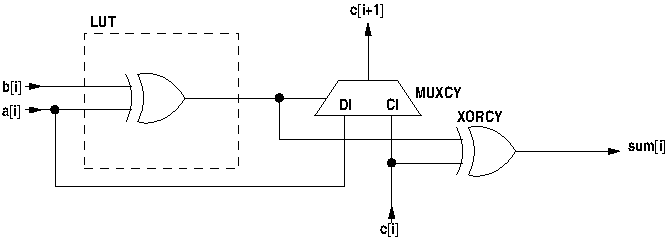
\includegraphics{add}
                    
                    If one of the operands is smaller than the other it is
                    padded with 0 if unsigned or the sign bit is extended if
                    signed. The sum is one bit wider than the operands.
                    
                    The carry in to the least significant bit is low. The carry
                    out of the most significant bit is the most significant bit
                    of the sum.

                    {\bf SUB} is a 2's complement subtraction. The logic
                    is the same as the adder except that the {\bf b} input
                    is inverted and the carry into the LSB is 1.                
                    
                    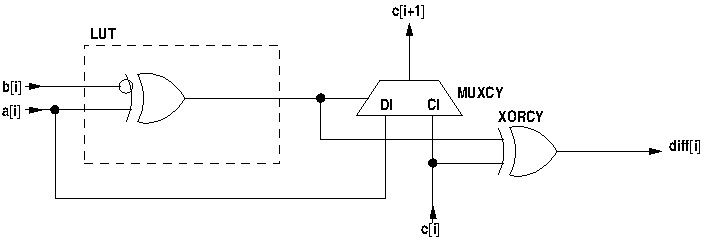
\includegraphics{sub}
                    
                    The {\bf igb} input gates the {\bf b} input as it does
                    in the adder however if the {\bf igb} input is used
                    it should also drive the LSB carry in because if
                    {\bf igb} is low the LSB carry in should be also low.

                    {\bf ADDSUB} is a combined adder/subtracter. The logic for
                    one stage is -

                    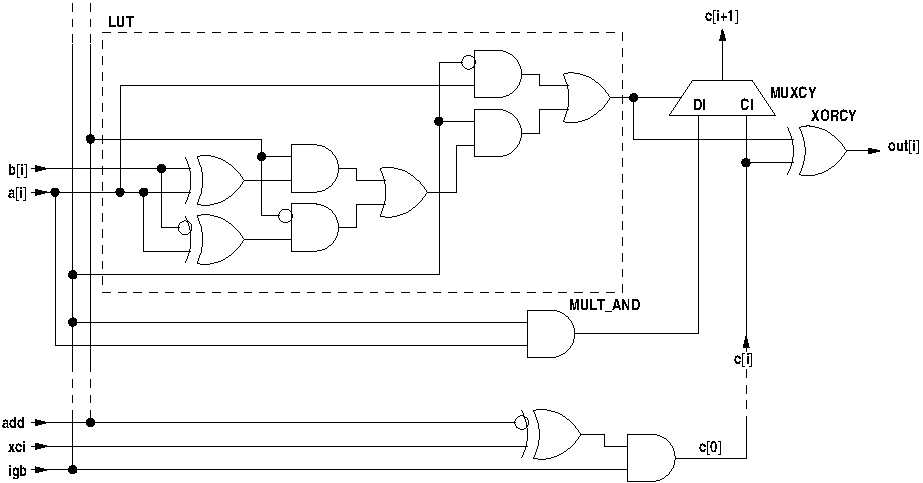
\includegraphics{addsub}
                    
                    If the {\bf igb} input is high and the {\bf add} input is
                    high the output is the sum of {\bf a} and {\bf b}. If the
                    {\bf add} input is low the output is the difference. If the
                    {\bf igb} input is low the output is {\bf a}. The {\bf xci} input
                    is XORed with the carry input.
                    
                    The LSB carry in is AND(XOR(NOT(add), xci), igb).
                    
                    {\bf ALU} is very similar to {\bf ADDSUB} but this operation
                    is intended as an ALU between a static variable and its
                    input selector for implementing v++, v--, v += n, v -= n and
                    v \verb'<'- n. The A input is connected to the variable output. The
                    gate control allows assignment of the B input for direct
                    assignment, rather than A +- B.
                    
                    The LSB carry in is AND(INV(add), iga).

                    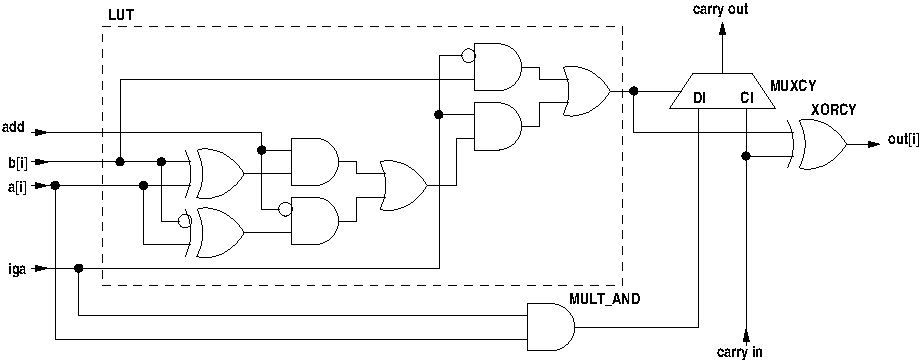
\includegraphics{alu}
                    
                    If the $5^{th}$ parameter is true then this ALU is input
                    to a static variable with the DSP attribute. If the
                    FPGA is a Virtex5 then a DSP48E will be used for the
                    ALU instead of the CLB logic previously illustrated.
                    The A input is connected to the C input of the DSP48E and
                    the B input is connected to the A input of the DSP48E.
                    The ALU mode and OP mode inputs are -

                    \begin{tabular}{| l | l | l |}
                    \hline
                    operation & ALU mode & OP mode \\
                    \hline
                    add       &   0000   & 0110011 \\
                    subtract  &   0011   & 0110011 \\
                    assign    &   0000   & 0110000 \\
                    \hline
                    \end{tabular}

                    {\bf MUL} is a 2's complement multiplier. For XC3S, XC2V and
                    XC2VP FPGAs the hardware multiplier is used. The operands
                    are restricted to a maximum of 18 bits. For a Virtex5 the
                    DSP48E multiplier is used and the operands are 18 and 25
                    bits.

                    For XC2S or XCV FPGAs the multiplier is implemented using
                    successive adders. There are separate multipliers for
                    unsigned and signed operands. This form of adder has a very
                    long combinatorial path and because of this is little used
                    since the clock rate is quite low (a few MHz). The logic is
                    not documented here.
                    

                    {\bf DIV}, {\bf REM} and{\bf DIVREM} all use the same
                    function which generates both the quotient and remainder in
                    2's complement arithmetic. There are separate signed and
                    unsigned versions. This function uses successive
                    adder/subtracters. It is even slower than the multiplier
                    described above. The logic is not documented here.

                    {\bf EQ} uses an XNOR of each pair of bits from the
                    two operands and ANDs the outputs to get the equality
                    output.

                    {\bf NE}  uses an XOR of each pair of bits from the
                    two operands and ORs the outputs to get the inequality
                    output.   

                    {\bf LT}, {\bf LE}, {\bf GT} and {\bf GE} all use
                    the {\bf GE} comparison by changing the operand order
                    and/or inverting the result. The {\bf GE} relational
                    operator uses the most significant bit of the difference
                    after subtraction.

                    {\bf AND}, {\bf OR} and {\bf XOR} use gates as one 
                    would expect, one per bit pair from the two operands.

                    {\bf LSH} and {\bf RSH} may have constant shift or variable
                    shift.
                    
                    Constant shift requires no logic and simply connects the
                    output signal array to the input signal array with an
                    offset. Left shifts connect least significant bits to zero.
                    Right shifts connect most significant bits to zero if
                    unsigned or to the input sign bit if signed.

                    Variable shifts use cascaded shifters, each shifting by a
                    power of two. Each shifting stage is controlled by one bit
                    of the shift count. The shifter is a 2-input multiplexer
                    using one LUT.

                    {\bf COND} implements the \verb'?:' operator and is simply a
                    2-input multiplexer per output bit, each multiplexer using
                    one LUT.


            \subsection{OR}

                \subsubsection{purpose}

                    An OR gate for control signals.

                \subsubsection{arguments}

                    \begin{tabular}{| l | l |}
                    \hline
                    Parameters  & none \\
                    \hline
                    Inputs      & input signal \\
                                & input signal \\
                                & . \\
                                & . \\
                    \hline
                    Outputs     & OR signal \\
                    \hline
                    \end{tabular}

                \subsubsection{description}

                    OR two or more input signals, the result appearing on the
                    output.

                \subsubsection{dump format}

                    \begin{lstlisting}[gobble=20, language=tde]
                        S11 = A12 | A14 | S8
                    \end{lstlisting}

                \subsubsection{logic description}

                    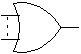
\includegraphics{or}

                    Xilinx implementation -

                    OR gates with 1 to 4 inputs will be implemented in a
                    single LUT (single input gates will be eliminated during
                    low-level code generation). OR gates with more than 4 inputs
                    use the carry chain to OR together the outputs of 1 to 4
                    input LUT OR gates (actually NOR gates).


        \subsection{PORT}

            \subsubsection{purpose}
            
                Flags a signal which is external to the current source code but
                is not external to the FPGA (i.e. not a pad connection). These
                signals are either connections to an imported core or are
                exported from the current source code which is itself a core.
                
            \subsubsection{arguments}
            
                \begin{tabular}{| l | l |}
                \hline
                Parameters  & Integer type of signal \\
                            & string  port name \\
                \hline
                Inputs      & signal or signal array \\
                \hline
                Outputs     & none \\
                \hline
                \end{tabular}

            \subsubsection{description}

                 The first parameter is an integer type code for the port type
                 which is 0 for input, 1 for output or 2 for 3-state output.
                 The second parameter is the port name.
            
            \subsubsection{dump format}
            
                \begin{lstlisting}{gobble=16, language={tde}}
                   PORT portname type signal
                \end{lstlisting}
                where {\em type} is "input", "output" or "3_state".


            \subsection{PRIORITY}

                \subsubsection{purpose}

                    A priority encoder.

                \subsubsection{arguments}

                    \begin{tabular}{| l | l |}
                    \hline
                    Parameters  & none \\
                    \hline
                    Inputs      & input signal array \\
                    \hline
                    Outputs     & output signal array \\
                                & else signal or null \\
                    \hline
                    \end{tabular}

                \subsubsection{description}

                When one or more inputs are high the highest priority matching
                output will be high and all other outputs low. The inputs are
                ordered in decreasing priority (the 1st is highest).

                The number of outputs is equal to the number of inputs or the
                number of inputs + 1. In the latter case the last output is
                the 'else' case, i.e. no inputs high.

                \subsubsection{dump format}

                    \begin{lstlisting}[gobble=20, language=tde]
                        PRIORITY {
                            in:
                                glob.a[0..2]
                            out:
                                prog.p[0..2]
                                prog.p.PE[0]
                        }
                    \end{lstlisting}

                \subsubsection{logic description}

                    Xilinx implementation -

                    The highest priority output is connected directly to its input.

                    For one input the optional ELSE output is the inverted input.

                    If the device is a CPLD the other outputs use AND gates.
                    If the device is an FPGA and the number of inputs is not
                    greater than the LUT width, LUTs are used.

                    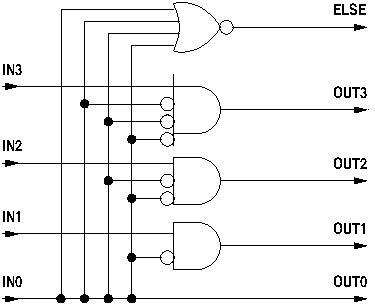
\includegraphics{priority1_4}

                    For FPGAs with more inputs than the LUT width the carry chain
                    is used. The implementation originally used the XORCY
                    element effectively as an AND gate. This was achieved by
                    ANDing the inverted input with the carry at each stage
                    and XORing the LIUT output and carry in.

                    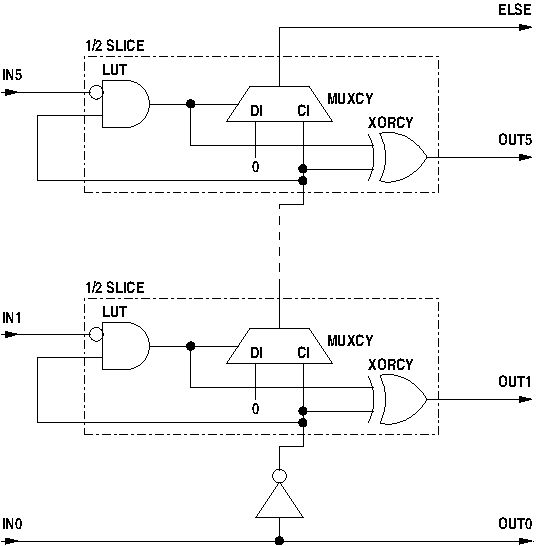
\includegraphics{priority5}
                    
                    This implementation was functionally correct however the
                    connection of each carry to the LUT input added a
                    significant delay to each stage, a delay much larger than
                    that of the carry chain itself. To eliminate this it
                    was necessary to depart from this rather neat solution
                    and instead add an external AND gate to each stage. These
                    AND gates add an extra delay to each stage but in parallel,
                    not cascaded. Hence the maximum path through the priority
                    encoder is very much shorter.

                    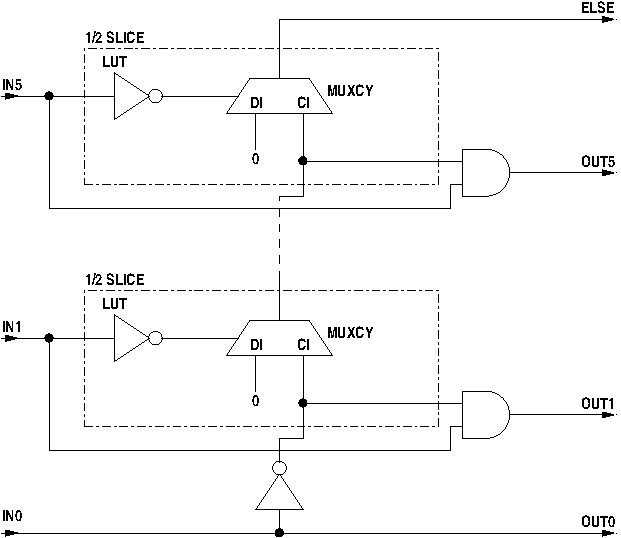
\includegraphics{priority6}


            \subsection{QUEUEBUFFER}

                \subsubsection{purpose}

                    A queue buffer.

                \subsubsection{arguments}

                    \begin{tabular}{| l | l |}
                    \hline
                    Parameters  & Integer depth \\
                                & Boolean use hardware FIFO is possible, or null \\
                                & String initial value (hexadecimal string) or null \\
                    \hline
                    Inputs      & input clock signal, or null if same as output clock \\
                                & output clock signal \\
                                & input data array \\
                                & push datum signal (.PUSH) \\
                                & pop datum signal (.POP) \\
                                & reset signal (optional) \\
                    \hline
                    Outputs     & output data array                          \\
                                & read available signal (.NE - not empty)  \\
                                & write available signal (.NF - not full)    \\
                                & ready availability signal for unbuffered queue \\
                                & synchronous buffer occupancy count or null \\
                                & synchronous buffer space count or null     \\
                                & asynchronous buffer write status           \\
                                & asynchronous buffer read status            \\
                                & reset signal (optional) \\
                    \hline
                    \end{tabular}

                \subsubsection{description}

                    A normal queue buffer has a depth of 2. If the depth is \verb'>' 2, an
                    initial value is not allowed. If a separate input clock is
                    supplied, depths start at 16 and are various powers of 2
                    depending on the size ranges of the block RAMs in the particular
                    FPGA. If the input data array and output data array arguments
                    are null then this is a null data queue buffer and the buffer
                    depth is a power of 2 greater than 3.
                
                    The 2nd output signal is the read availability signal. This is
                    high if the buffered queue is not empty. For an unbuffered queue
                    it is high if the queue is waiting on a write.

                    The 3rd output signal is the write availability signal. This is
                    high if the buffered queue is not full. For an unbuffered queue
                    it is high if the queue is waiting on a read, i.e. it is
                    connected to the POP input.

                    The 4th output is null for a buffered queue. For an unbuffered
                    queue it is the AND of the push (write) and pop (read) inputs
                    (which is also the AND of the read availability (NE) and write
                    availability (NF) signals.

                    If the 5th output is not null this gives the number of words in
                    a synchronous queue buffer synchronised to the queue clock (read
                    and write).

                    If the 6th output is not null this gives the number of free
                    spaces in a synchronous queue buffer synchronised to the queue
                    clock (read and write).

                    If the 7th output is not null this gives the buffer status for
                    an asynchronous queue buffer synchronised to the write (input)
                    clock.

                    If the 8th output is not null this gives the buffer status for
                    an asynchronous queue buffer synchronised to the read (output)
                    clock.

                    If there is an 9th output this is a reset signal. This
                    signal goes high for one clock cycle when the queuebuffer is
                    reset via the reset() inbuilt procedure. For an asynchronous
                    queuebuffer this signal is synchronised to the read (output)
                    clock and is timed to follow the reset of the input (write)
                    side of the queuebuffer.

                    The asynchronous queue buffer status is a 5-bit word
                    whose bits are -
                    \blist
                    \item   bit 0 - empty to 1/4 full + 1    
                    \item   bit 1 - 2 words to 1/2 full  + 1  
                    \item   bit 2 - 1/4 full + 1 to 3/4 full  + 1
                    \item   bit 3 - 1/2 full + 1 to full     
                    \item   bit 4 - 3/4 full + 1 to full     
                    \blend
                    The bits are mutually exclusive and one of them is always set.


                    Synchronous data queue buffers have a default depth of 2.
                    Synchronous null queue buffers have a default depth of 16.
                    Asynchronous data queue buffers have a default depth of 16.
                    Asynchronous null queue buffers have a default depth of 16. Null
                    queue buffers may have a depth which is 4 or greater and which is
                    a power of 2. Data queue buffers may have the following depths -
                    \blist
                    \item   Virtex - 16, 256, 512, 1024, 2048 or 4096
                    \item   Virtex-II - 16, 512, 1024, 2048 or 4096, 8192 or 16384
                    \blend
                    and for synchronous buffers depth 2 is also allowed and is
                    the default.

                \subsubsection{dump format}

                    \begin{lstlisting}[gobble=20, language=tde]
                        QUEUEBUFFER (512)
                            OUT    glob.frontend_0.i1[0..7,8]
                            NE     glob.frontend_0.i1.NE[0]
                            NF     glob.frontend_0.i1.NF[0]
                            CNT    null
                            SPC    null
                            WSTAT  null
                            RSTAT  glob.frontend_0.i1.RSTAT[0,1,2,3,4]
                            <-
                            CLKIN  glob.sdclk0
                            CLKOUT glob.c100
                            DATA   glob.frontend_0.i1.D[0..7,8]
                            PUSH   glob.frontend_0.i1.PUSH
                            POP    glob.frontend_0.i1.POP
                            R      glob.frontend_0.i1.RES
                    \end{lstlisting}

                    The minimum size of the buffer is two and this is implemented as
                    two registers. {\bf NF} stands for ''Not Full``, meaning
                    that at least one free register is available for writing. {\bf
                    PUSH} stands for ''push data onto queue``. {\bf NE}
                    stands for ''Not Empty``, meaning one or more registers contains
                    data which can be read. {\bf POP} acknowledges a read, popping
                    the word from the buffer (queue).

                \subsubsection{logic description}

                    There are five separate implementations of queue buffers -
                    \blist
                    \item   a synchronous queue buffer of depth two (default)
                    \item   a synchronous queue buffer of depth greater than two
                    \item   an asynchronous queue buffer
                    \item   a asynchronous or asynchronous queue buffer with no data
                    \item   a asynchronous or asynchronous queue buffer of depth 0
                    \blend

                    The logic for the default synchronous queue buffer of depth
                    two is -

                    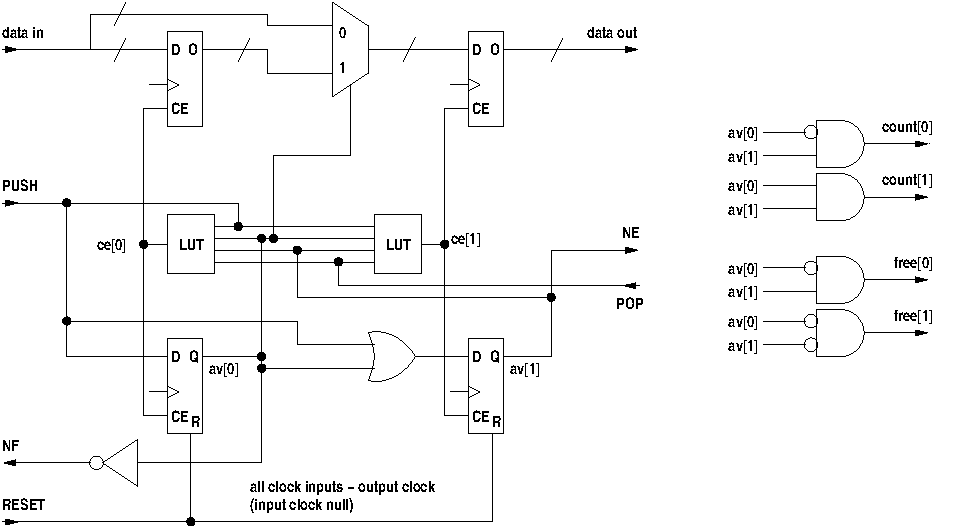
\includegraphics{queuebuffer}

                    The 2-input multiplexer shown uses a 3-input LUT per bit.

                    When PUSH is high input data is latched into one of two
                    registers. If the buffer is empty the data is latched into the
                    rightmost register to which the data output is directly
                    connected. If another datum is written to the queue buffer it
                    goes into the second (left) register. When a datum is
                    popped the two registers are shifted right. This
                    scheme avoids having combinatorial logic at the output thus
                    minimising clock-to-data-out time. The tradeoff is a longer
                    input setup time. The two flip-flops represent the occupancy
                    status of the two registers. Each register/flip-flop pair has a
                    common clock enable controlled by a 4-input LUT.

                    The truth table for the control logic is as follows -

                    \begin{tabular}{ | c | c | c | c | | c | c | c | | c | c | c | c | c | c | l }
                    \cline{1-13}
                    \multicolumn{7}{| c ||}{t} & \multicolumn{6}{ c |}{t+1} & \\
                    \cline{1-13}
                      &    & \multicolumn{2}{ c ||}{av} & \multicolumn{2}{ c |}{ce} & & \multicolumn{2}{ c |}{av}
                      & \multicolumn{2}{ c |}{ce} & & & \\
                    PUSH & POP & [0] & [1] & [0] & [1] & MUX & [0] & [1] & [0] & [1] & NE & NF & \\
                    \cline{1-13}
                    \cline{1-13}
                    0 & 0 & 0 & 0 & 0 & 0 & X & 0 & 0 & 0 & 0 & 0 & 1 & empty \\
                      &   & 0 & 1 & 0 & 0 & X & 0 & 1 & 0 & 1 & 1 & 1 & 1 entry \\
                      &   & 1 & 0 & - & - & - & - & - & - & - & - & - & illegal state \\
                      &   & 1 & 1 & 0 & 0 & X & 1 & 1 & 1 & 1 & 1 & 0 & full \\
                    \cline{1-13}
                    0 & 1 & 0 & 0 & - & - & - & - & - & - & - & - & - & illegal state \\
                      &   & 0 & 1 & X & 1 & X & 0 & 0 & 0 & 0 & 0 & 1 & av[1] $\downarrow$ POP, now empty\\
                      &   & 1 & 0 & - & - & - & - & - & - & - & - & - & illegal state \\
                      &   & 1 & 1 & 1 & 1 & 1 & 0 & 1 & 0 & 1 & 1 & 1 & av[0] $\downarrow$ POP, 1 remaining\\
                    \cline{1-13}
                    1 & 0 & 0 & 0 & 0 & 1 & 0 & 0 & 1 & 0 & 1 & 1 & 1 & av[1] $\uparrow$ PUSH, 1 entry\\
                      &   & 0 & 1 & 1 & 0 & X & 1 & 1 & 1 & 1 & 1 & 0 & av[0] $\uparrow$ PUSH, now full\\
                      &   & 1 & 0 & - & - & - & - & - & - & - & - & - & illegal state \\
                      &   & 1 & 1 & - & - & - & - & - & - & - & - & - & illegal state \\
                    \cline{1-13}
                    1 & 1 & 0 & 0 & - & - & - & - & - & - & - & - & - & illegal state \\
                      &   & 0 & 1 & 0 & 1 & 0 & 0 & 1 & 0 & 1 & 1 & 1 & 1 entry \\
                      &   & 1 & 0 & - & - & - & - & - & - & - & - & - & illegal state \\
                      &   & 1 & 1 & - & - & - & - & - & - & - & - & - & illegal state \\
                    \cline{1-13}
                    \end{tabular}

                    {\bf PUSH} must not be raised when
                    {\bf NF} is low and {\bf POP} must not be raised when
                    {\bf NE} is low.

                    The illegal states are described in the following table

                    \begin{tabular}{ c | c | c | c | c || l | }
                    \multicolumn{6}{ c }{illegal states} \\
                    & PUSH & POP & av[0] & av[1]  \\
                    \hline
                    1 & 0 & 0 & 1 & 0 & single entry must be at right  \\
                    2 & 0 & 1 & 0 & 0 & cannot pop when empty  \\
                    3 & 0 & 1 & 1 & 0 & single entry must be at right  \\
                    4 & 1 & 0 & 1 & 0 & single entry must be at right  \\
                    5 & 1 & 0 & 1 & 1 & cannot push when full  \\
                    6 & 1 & 1 & 0 & 0 & cannot pop when empty  \\
                    7 & 1 & 1 & 1 & 0 & single entry must be at right  \\
                    8 & 1 & 1 & 1 & 1 & cannot push when full  \\
                    \hline
                    \end{tabular}

                    In entries 1, 3, 4 and 7 a single datum in the buffer must
                    reside in the right register, so these states are not
                    allowed.

                    In entry 2 the registers are both empty and so a {\bf POP}
                    is not allowed since there is no valid output ({\bf NE} is
                    low). The logic has been designed so that no state change
                    occurs, i.e. the {\bf POP} is ignored.

                    In entry 6 the registers are both empty and so a {\bf POP}
                    is not allowed since there is no valid output ({\bf NE} is
                    low), however {\bf PUSH} is high. The logic has been designed
                    so that the {\bf PUSH} is handled but the {\bf POP} is
                    ignored.

                    In entries 5 and 8 both registers are full and hence no {\bf
                    PUSH} is allowed. Note that this is true even when {\bf POP}
                    is asserted since we cannot allow {\bf NF} (not full) to
                    depend on {\bf POP} or we generate the very logic cascade
                    this buffering scheme was designed to avoid. The logic has
                    been designed to ignore {\bf PUSH} in these cases.

                    The truth tables for the two LUTs are -

                    \begin{tabular}{ l || c | c | c | c |}
                    & PUSH & POP & av[0] & av[1]  \\
                    \hline
                    ce[0] & 0 & 1 & 1 & 1 \\
                          & 1 & 0 & 0 & 1 \\
                    \hline
                    ce[1] & 0 & 1 & X & 1 \\
                          & 1 & X & 0 & 0 \\
                          & 1 & 1 & 0 & 1 \\
                    \hline
                    \end{tabular}



                    A synchronous queue buffer of depth greater than two is
                    implemented using either CLB dual port RAM or dual port
                    block RAM. The CLB RAM is used for a depth of 16 and block
                    RAM for greater depths.
                    
                    Because CLB RAM has combinatorial output and block RAM
                    has registered output the CLB RAM is employed with a
                    register appended to the output port so that the two
                    forms of RAM can be used interchangably with the same
                    control logic.
                    
                    The queue buffer is a queue. A required characteristic of
                    queue buffers is that on writing a datum to an empty queue
                    buffer that datum must be available on the next clock cycle.
                    This presents a problem with a dual-port FIFO using
                    registered output RAM because a read must be issued once the
                    queue becomes non-empty, taking an extra cycle. This can be
                    avoided by writing the first datum into a separate register
                    rather than into the empty RAM. For CLB RAM this is easily
                    implemented however in the case of block RAM the control
                    logic for this is somewhat complicated. An easier solution
                    for block RAM is to write the first datum into an empty
                    queue via the read port rather than the write port. Since
                    the queue is empty the read port is guaranteed to be unused
                    on that clock cycle. Since the normal write mode for block
                    RAM is WRITE\_FIRST and the CLB RAM with appended output
                    register has been designed to behave the same way, the newly
                    written datum will appear immediately in the output register
                    upon writing. This avoids the extra cycle.
                    
                    For a block RAM the memory logic is -

                    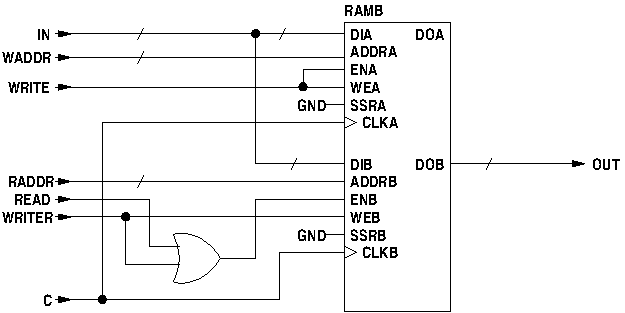
\includegraphics{qbram}
                    
                    To make an equivalent functional unit using CLB RAM
                    the logic is -

                    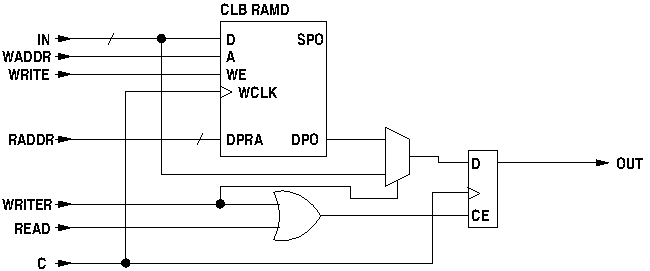
\includegraphics{qcram}
                    
                    In both the above blocks {\bf WRITER} writes directly to the
                    output register whereas {\bf WRITE} writes to the RAM. {\bf
                    READ} reads from the RAM to the output register.

                    The following terms are used in the logic description -
                    
                    \blist
                    \item   empty - the RAM is empty
                    \item   full - the RAM is full
                    \item   NE - data is available at the output of the queue buffer
                    \item   NF - data can be written to the queue buffer
                    \item   read - read RAM
                    \item   write - write RAM
                    \item   writer - first write when queue buffer empty
                    \item   raddr - RAM read address
                    \item   waddr - RAM write address
                    \item   fcnt - RAM occupancy counter
                    \item   $\Uparrow$ - increment
                    \item   $\Downarrow$ - decrement
                    \blend
                    
                    Note that a RAM occupancy counter, {\bf fcnt}, is kept in
                    addition to read and write address counters. {\bf fcnt} is
                    used to determine the RAM full and empty conditions and is
                    potentially faster than doing comparisons between {\bf
                    raddr} and {\bf waddr}. Additional counters are used for the
                    optional word count and space count, again trading speed for
                    logic and routing resources.
                    
                    The following table shows the change of state and counter
                    increment/decrement operations in controlling the queue
                    buffer ({\bf full} and {\bf NF} are not shown) -

                    \begin{tabular}{ | c | c | c | c || c | c | c | c | c | c | c |}
                    \hline
                    \multicolumn{2}{| c |}{state} &
                    \multicolumn{2}{ c ||}{inputs} &
                    \multicolumn{3}{ c |}{increment/decrement} &
                    \multicolumn{3}{ c |}{memory control} &
                    new \\
                    \cline{1-10}
                    empty & NE & PUSH & POP & waddr & raddr & fcnt & write & writer & read & NE\\
                    \hline
                    1 & 0 & 1 & 0 &            &            &              & 0 & 1 & 0 & 1 \\                     
                    0 & 1 & 1 & 0 & $\Uparrow$ &            & $\Uparrow$   & 1 & 0 & 0 & 1 \\           
                    1 & 1 & 1 & 0 & $\Uparrow$ &            & $\Uparrow$   & 1 & 0 & 0 & 1 \\           
                    0 & 1 & 1 & 1 & $\Uparrow$ & $\Uparrow$ &              & 1 & 0 & 1 & 1 \\           
                    1 & 1 & 1 & 1 &            &            &              & 0 & 1 & 0 & 1 \\                     
                    0 & 1 & 0 & 1 &            & $\Uparrow$ & $\Downarrow$ & 0 & 0 & 1 & 1 \\       
                    1 & 1 & 0 & 1 &            &            &              & 0 & 0 & 0 & 0 \\                    
                    \hline
                    \end{tabular}
                    
                    On first write to an empty queue buffer the datum is
                    written directly to the read port of the RAM block and
                    {\bf NE} goes high, but {\bf fcnt} stays at 0 as nothing is
                    written to the RAM. The next write (if there is no read) will
                    write to RAM and increment both{\bf fcnt} and {\bf waddr}. On
                    acknowledging the output datum (i.e. popping a datum off
                    the queue) if there is only the datum in the read port register
                    {\bf NE} will go low since {\bf fcnt} is 0 ({\bf empty}
                    will be true). If there is a datum in the output register and
                    another in the RAM then the last RAM read to the port register
                    will occur and {\bf fcnt} will decrement from 1 to 0 and
                    empty will become true, but NE will not go low until the next
                    {\bf POP}.
                    
                    Related equations -
                    
                    % NF = !full
                    % read = POP & !empty
                    % write = PUSH & NE & !(empty & POP)
                    % writer = PUSH & empty & !(NE & !POP)                  
                    $
                    \mathsf{NF = \overline{full}} \\
                    \mathsf{read = POP \cdot \overline{empty}} \\
                    \mathsf{write = PUSH \cdot NE \cdot \overline{(empty \cdot POP)}} \\
                    \mathsf{writer = PUSH \cdot empty \cdot \overline{(NE \cdot \overline{POP})}}
                    $
                    
                    State changes -
                    
                    % NE <- !(empty & NE & !PUSH & POP)
                    % empty <- !write & (fcnt==0 | fcnt==1 && read)
                    % full <- !read & (fcnt==11...11 | fcnt==11...10 & write)
                    $
                    \mathsf{NE \Leftarrow \overline{empty \cdot NE \cdot \overline{PUSH} \cdot POP}} \\
                    \mathsf{empty \Leftarrow \overline{write} \cdot (fcnt==0 + fcnt==1 \cdot read)} \\
                    \mathsf{full \Leftarrow \overline{read} \cdot (fcnt==11\cdots11 + fcnt==11\cdots10 \cdot write)}
                    $
                    
                    Increment/decrement counters -

                    % raddr++ = read
                    % waddr++ = write
                    % fcnt++ = write & !read
                    % fcnt-- = read & !write
                    $
                    \mathsf{raddr\Uparrow = read} \\
                    \mathsf{waddr\Uparrow = write} \\
                    \mathsf{fcnt\Uparrow = write \cdot \overline{read}} \\
                    \mathsf{fcnt\Downarrow = read \cdot \overline{write}}
                    $

                    For an asynchronous queue buffer the input and output clocks
                    differ and the scheme for avoiding an initial read on a
                    write to an empty queue buffer cannot be used. The point at
                    which a queue becomes available after a write to an empty
                    buffer is now undefined since the clocks are separate and
                    unrelated.

                    The CLB RAM block now simply has a register on the output
                    of the read-only port.

                    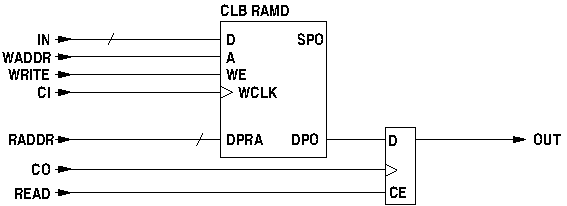
\includegraphics{aqcram}
                    
                    The block RAM has no additional logic.

                    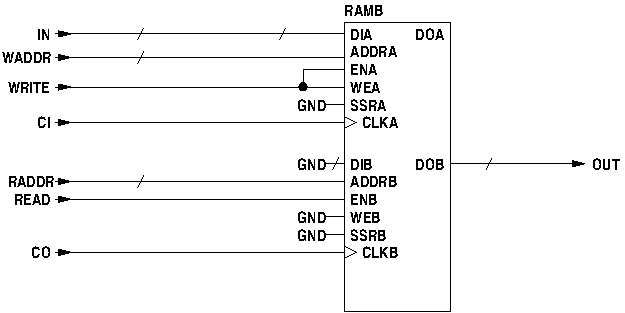
\includegraphics{aqbram}
                    
                    The asynchronous queue buffer uses one of the above RAMs (the
                    former for depth 16, the latter for greater depths) and an
                    address generator block. The use of address comparison for
                    full and empty determination means that the depth of the RAM
                    FIFO is $2^n - 1$ however an additional datum is held in the
                    RAM output register giving a total buffer depth of $2^n$.
                    The additional logic shown provides the first read following
                    a write to an empty buffer after which {\bf NE} is raised.

                    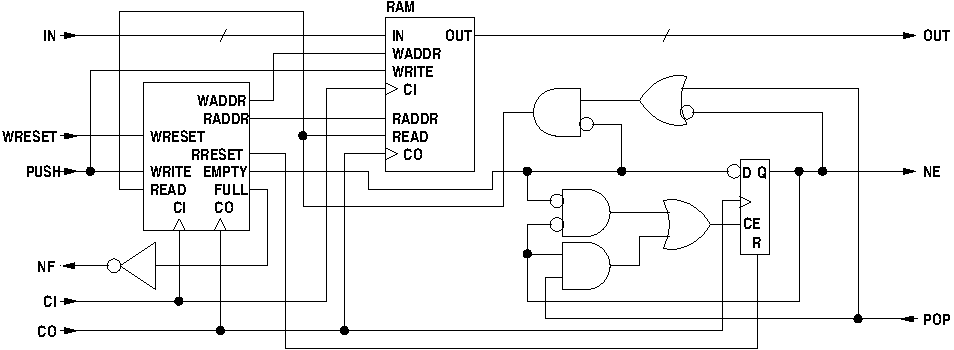
\includegraphics{asyncqueuebuffer}
                    
                    Resetting an asynchronous queue buffer must be carried out with
                    care. A pending read must be allowed to complete after which
                    {\bf NE} will go low and no more reads will occur (since the
                    queue buffer is now empty). A pending write must be ignored and
                    {\bf NF} forced low (the source will now remove {\bf PUSH},
                    withdrawing the write request). {\bf NF} must remain low during
                    the reset process (which may be many cycles if the input clock
                    is higher than the output clock) and then go high when the now
                    empty queue buffer is again available for writing.
                    
                    The reset input is synchronised to the write (input) clock.
                    When asserted it resets the write address and clears the
                    full flip-flop (and holds it clear during the reset
                    process). At the same time it sets a blocking flip-flop to
                    force {\bf NF} low so that a write will not occur (the reset
                    also immediately forces {\bf NF} low to supress a possible
                    write in the current cycle). The reset is resynchronised to
                    the read (output) clock to later reset the read address, the
                    empty flip-flop and the {\bf NE} flag. A further pulse is
                    then generated once again in the input clock domain to
                    finally free the blocking flip-flop and raise {\bf NF} after
                    the output side has been reset. This mechanism is necessary
                    to avoid attempts to write to the buffer before the output
                    side is reset. On the other hand the output side reset must
                    be synchronised to the output clock so that it can fit in
                    with pending reads, lowering {\bf NE} synchronously with the
                    output to stop further reads.
                    
                    If the queue buffer is never reset the reset logic
                    is omitted.
                    
                    The address generator follows the design given in Xilinx
                    application note 131.

                    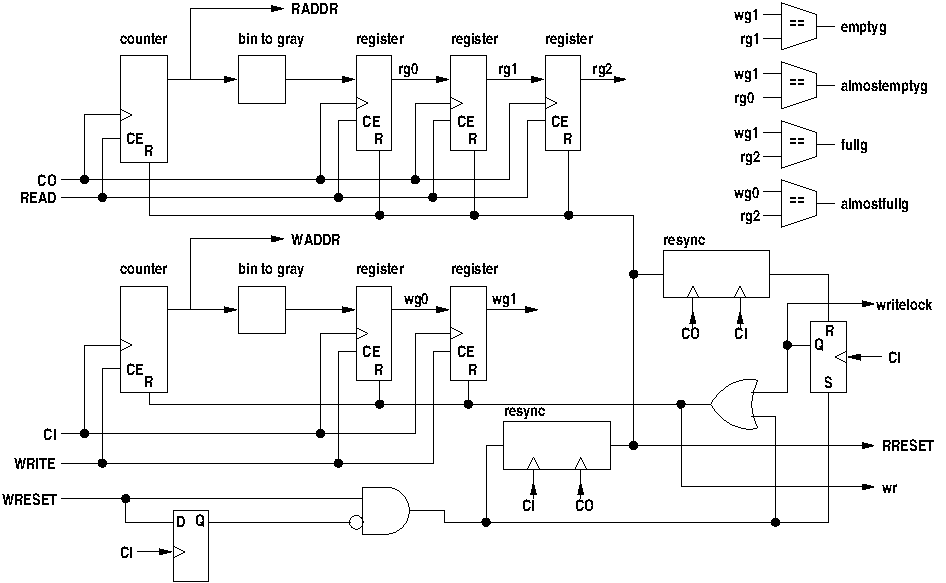
\includegraphics{asyncaddr}
                    
                    When {\bf WRESET} is asserted it resets the write address
                    counter to zero and the following grey code registers
                    to the initial values -

                    \begin{tabular}{c c}
                    wg0 & 100...000 \\
                    wg1 & 100...001 \\
                    \end{tabular}

                    At the same time it is gated through to {\bf FULL} and
                    also latched in a flip-flop so that
                    the queuebuffer appears full and will not be written on the
                    current or subsequent clock cycles. The write reset is
                    resynchronised to the read clock and the resulting signal
                    is output to {\bf RRESET} for possible daisy chaining to
                    further queues in the pipeline. {\bf RRESET} also resets the
                    {\bf EMPTY} flip-flop,
                    resets the read address counter to zero and the following
                    grey code registers to the initial values -

                    \begin{tabular}{c c}
                    rg0 & 100...000 \\
                    rg1 & 100...001 \\
                    rg2 & 100...011 \\
                    \end{tabular}
                    
                    These initial values on the write and read sides ensure the
                    queue buffer appears initially empty and empty after a reset.
                    The values are the gray code sequence leading up to the
                    current read and write addresses of 0 (gray code 0) and
                    hence are gray code equivalents of -1, -2 and -3.
                    
                    {\bf RRESET} is then resynchronised back to the write
                    clock and resets the flip-flop holding {\bf FULL} asserted.
                    The reset process thus takes a number of read and write
                    clock cycles, the exact duration depending on the two clock
                    frequencies. The reset inhibits any writes on the current
                    clock cycle and from then on until the reset is complete.
                    The queue buffer does not appear empty immediately the
                    reset is asserted on the write side, however only one read
                    can take place (if the queue buffer is not already empty) and
                    that will read a correct datum. After that the queue buffer
                    will be reset on the read side and will appear empty. The
                    queue buffer can then only appear non-empty after a
                    subsequent write following the reset.

                    The gray code address comparisons at various phases are
                    compared to determine empty and full conditions -

                    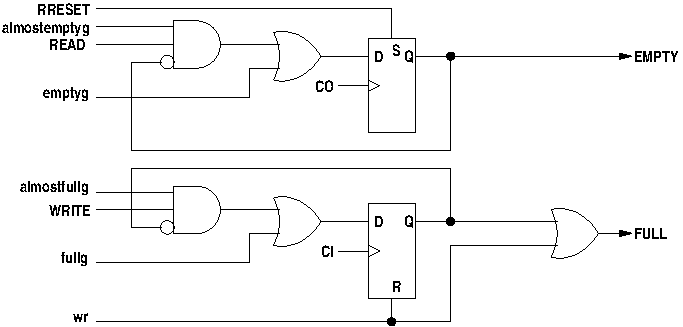
\includegraphics{asyncfullempty}
                   
                    The binary to gray code converter logic is -

                    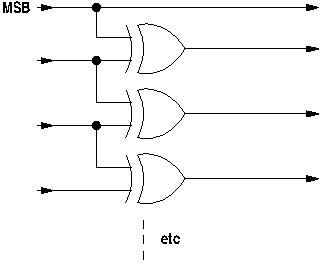
\includegraphics{bintogray}
            
                    A (synchronous) unbuffered queue is created by connecting the
                    {\bf NE} (not empty) output net to the {\bf PUSH} input net and
                    the {\bf NF} (not full) output net to the {\bf POP} input net.
                    Since the functionality of an unbuffered queue differs
                    substantially from that of a buffered queue the inputs and
                    outputs are better labelled {\bf WRITE} for {\bf PUSH}, {\bf
                    READ} for {\bf POP}, {\bf WAV} for {\bf NF} and {\bf RAV} for
                    {\bf NE}.
                    
                    With these cross connections asserting the {\bf WRITE} input
                    asserts the {\bf RAV} output and the queue now has read
                    availability. In the same way asserting the {\bf READ} input
                    asserts the {\bf WAV} output and the queue now exhibits write
                    availability. The {\bf WRITE} is driven by the {\bf WPENDING}
                    output of an EXECP and the {\bf READ} is driven by the {\bf
                    RPENDING} output of an EXECP. This is described
                    later (\ref{ubqueuerw}). The data output is simply connected
                    to the data input as the unbuffered queue does not store
                    anything.
                    
                     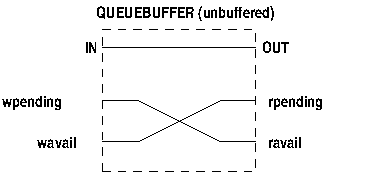
\includegraphics{ubqueue}
                     
                     Where an unbuffered queue is written or read in more than one
                     place in the source code the {\bf WRITE} and {\bf READ} inputs
                     are the PENDING signals from the different EXECPs ORed.
              
 

            \subsection{REG}

                \subsubsection{purpose}

                    A register (static variable).

                \subsubsection{arguments}

                    \begin{tabular}{| l | l |}
                    \hline
                    Parameters  & String[] - block ids \\
                                & String - initial value \\
                                & boolean - IOB flag \\
                                & boolean - DSP flag \\
                    \hline
                    Inputs      & clock signal (may be null if .D null) \\
                                & data signal array (.D - may be null) \\
                                & clock enable signal or signal array (.CE) \\
                                & set/reset signal or signal array (.RES) \\
                    \hline
                    Outputs     & data signal array \\
                    \hline
                    \end{tabular}

                \subsubsection{description}

                    When the clock enable is high data will be clocked in on
                    the next clock edge. For a primitive type all clock enable
                    inputs are tied together as are all reset inputs. For
                    a compound type clock enables and resets are grouped in words
                    corresponding to primitives. The resets return the state to
                    the initial value (0 by default).
                    If the clock is null, there are no inputs to
                    this register so generate a constant instead.
                
                    Optional attributes are -
                    \begin{tabular}{| l | l |}
                    \hline
                    timingname  & timing group name \\
                    loc         & flip-flop location \\
                    iob         & place flip-flop(s) in IOB(s) \\
                    \hline
                    \end{tabular}
                    If any {\bf loc} attributes are provided there must be a {\bf loc} entry per bit.
                    These are ordered from the LSB.

                \subsubsection{dump format}

                    \begin{lstlisting}[gobble=20, language=tde]
                        REG
                            OUT  glob.v[0..7]
                            <-
                            CLK  glob.c100
                            DATA glob.v.D[0..7]
                            CE   glob.v.CE[0..7]
                            R    glob.v.RES[0..7]
                            {0x0}{timingname=reg1}
                    \end{lstlisting}
                    The last line shows the initial value folowed by any attributes.

                \subsubsection{logic description}

                    If the clock input is null a constant is generated and the
                    other inputs are ignored, otherwise each output bit has a
                    D-type flip-flop. The data input must be the same width as
                    the output. The clock enable and reset inputs may be arrays
                    in which case they must be the same width as the input and
                    output. Alternatively they may both be width 1 in which case
                    all bits will share the same clock enable and reset. Either
                    or both may be null.
                
                    Optional attributes are -
                    \begin{tabular}{| l | l | l |}
                    \hline
                    timingname  & "str"            & timing group name \\
                    loc         & "str" or "[]str" & flip-flop location(s) \\
                    iob         & "log"            & place flip-flop(s) in IOB(s) \\
                    \hline
                    \end{tabular}


            \subsection{RESYNC}

                \subsubsection{purpose}

                    A pulse or level resynchroniser.

                \subsubsection{arguments}

                    \begin{tabular}{| l | l |}
                    \hline
                    Parameters  & none \\
                    \hline
                    Inputs      & input signal \\
                                & input clock signal \\
                                & output clock signal \\
                    \hline
                    Outputs     & output signal \\
                    \hline
                    \end{tabular}

                \subsubsection{description}

                    The input may be a pulse or a level. When the input rises the
                    rise is captured by the next input clock edge and an output
                    pulse of one period duration is generated on the next output
                    clock edge.

                \subsubsection{dump format}

                    \begin{lstlisting}[gobble=20, language=tde]
                        RESYNC {
                            in:
                                glob.a[0]
                                glob.c100
                                glob.bus_clk
                            out:
                                E41[0]
                        }
                    \end{lstlisting}

                \subsubsection{logic description}

                    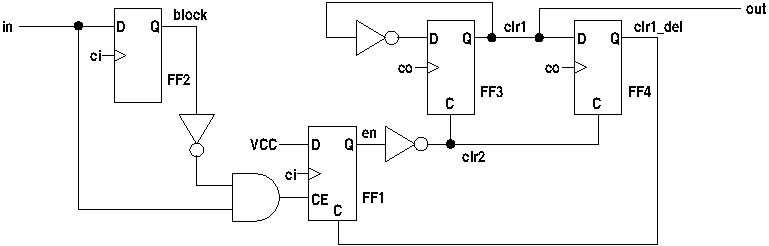
\includegraphics{resync}

                    Note that FF1, FF3 and FF4 have asynchronous clear inputs. Initially
                    all flip-flop outputs are low, thus {\bf block} and {\bf clr1}/{\bf
                    out} are low. When {\bf in} goes high both FF1 and FF2 outputs go
                    high on the next edge of clock {\bf ci}, the input clock. The {\bf
                    CE} input of FF1 goes low as {\bf block} is now high. Since {\bf en}
                    is now high, {\bf clr2} is low and this enables FF3 to toggle on the
                    next edge of {\bf co}, the output clock, raising the output {\bf
                    out}. On the next edge of {\bf co} FF3 toggles low again and FF4 is
                    set, raising {\bf clr1\_del}, which clears FF1. When {\bf en} thus
                    goes low {\bf clr2} goes high clamping FF3 low and clearing FF4. FF1
                    is now free to again latch an input however if {\bf in} is still
                    high {\bf block} will disable FF1. Thus {\bf in} must be clocked low
                    to lower {\bf block} before FF1 can again start the pulse cycle.
                    This circuit avoids race conditions between flip-flops in the two
                    clock domains.


            \subsection{RRAM}

                \subsubsection{purpose}

                    Registered-output RAM.

                \subsubsection{arguments}

                    \begin{tabular}{| l | l |}
                    \hline
                    Parameters  & Integer number of ports \\
                                & Integer data width in bits \\
                                & Integer address width in bits \\
                                & String[] optional initialisation \\
                                & String - attribute key \\
                                & String - data for attribute key \\
                                &       ...     other attribute pairs \\
                    \hline
                    Inputs      & clock signal, port0 \\
                                & address array, port0 \\
                                & data\_in array, or null, port0 \\
                                & read signal, or null, port0 \\
                                & write signal, or null, port0 \\
                                & clock signal, port1 \\
                                & address array, port1 \\
                                & data\_in array, or null, port1 \\
                                & read signal, or null, port1 \\
                                & write signal, or null, port1 \\
                                & ..etc.. \\
                    \hline
                    Outputs     & data\_out array, or null, port0 \\
                                & data\_out array, or null, port1 \\
                    \hline
                    \end{tabular}

                \subsubsection{description}

                    This is a RAM with clocked read and write. The output for a
                    port reflects the memory contents following a read clock
                    cycle.

                    The 2nd parameter gives the data width and the address width
                    gives the memory depth (number of words). All port addresses
                    must be the same width and all port data inputs and outputs
                    must be the same width.

                    The initialisation string array has one entry for each
                    initial value. Each entry is a hexadecimal string. The
                    initialisation array may be smaller than the depth of the
                    RAM but not larger. The initialisation parameter may be
                    omitted in which case the RAM is explicitly initialised to
                    all 0.

                    Other attributes ({\bf writemode}, {\bf writemodea}, {\bf
                    writemodeb}, {\bf timingname}) if set result in entries
                    written to the NCF file.

                    Ports which are not written have null arguments for the data
                    in and the write enable. Ports which are not read have null
                    arguments for the data out.

                    For Xilinx FPGAs registered-output RAM is block RAM. The
                    address width is limited to a maximum of 12 bits (a depth of
                    4096 words) for Spartan 2, Virtex and  Virtex E and 14 bits
                    (a depth of 16384 words) for Spartan 3, Virtex 2 and Virtex
                    2 PRO. The data width is not limited.
                
                    Attributes are -
                    
                    \begin{tabular}{| l | l |}
                    \hline
                    loc             & block RAM location \\
                    timingname      & timing group name \\
                    writemode       & write mode \\
                    writemodea      & port A write mode \\
                    writemodeb      & port B write mode \\
                    continuous      & continuous enable \\           
                    \hline
                    \end{tabular}
                    
                    There is one {\bf loc} attribute per block. Block RAM formats
                    are selected by address width, then the number of blocks is
                    determined by the total data width divided by the block data width.
                    Block locations are in order from the least significant data bits.
                    The other attributes are be applied to each
                    individual RAMB4\_S, RAMB4\_S\_S, RAMB16\_S or
                    RAMB16\_S\_S prepended in each case with "INST name "
                    where 'name' is the generated netlist identifier for the
                    RAM component.

                \subsubsection{dump format}

                    \begin{lstlisting}[gobble=20, language=tde]
                        RRAM - 2 ports
                            OUT  glob.pileup_0.tmin_0[0..7]
                            OUT  glob.pileup_0.tmin_1[0..7]
                            <-
                            CLK  glob.c100
                            ADDR S5309[0..11]
                            DATA null
                            RE   S5310
                            WE   null
                            CLK  glob.c100
                            ADDR S5311[0..11]
                            DATA S5313[0..7]
                            RE   null
                            WE   S5312
                        initialised{continuous=true}
                    \end{lstlisting}

                    The presence of an initialisation argument is flagged
                    but the values are not listed.

                \subsubsection{logic description}

                    For Xilinx registered output RAM is block RAM. The register
                    reset input is unused and the enable input is {\bf READ}
                    OR {\bf WRITE} (gate omitted if only one of these inputs is
                    used). BRAM ports are configured for the address width (if
                    two ports they must be the same width) and the data width
                    is matched by using as many blocks in parallel as required.
                    WRITE\_MODE is the default WRITE\_FIRST.
                    
                    For single port BRAM -

                    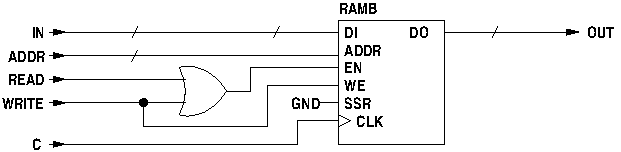
\includegraphics{bram1}
                    
                    and for two port BRAM -
                    
                    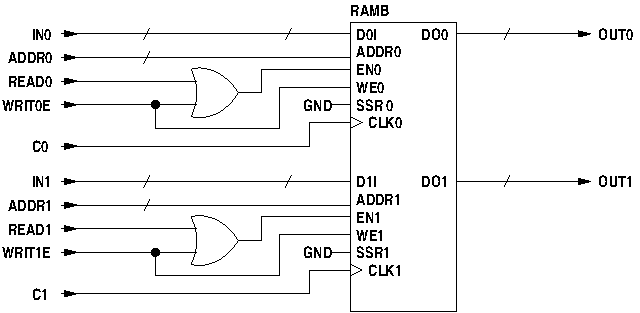
\includegraphics{bram2}


            \subsection{SAMPLE}

                \subsubsection{purpose}

                    Sample data from a different clock domain.

                \subsubsection{arguments}

                    \begin{tabular}{| l | l |}
                    \hline
                    Parameters  & none \\
                    \hline
                    Inputs      & input data array \\
                                & input clock signal \\
                                & output clock signal \\
                    \hline
                    Outputs     & output data array \\
                    \hline
                    \end{tabular}

                \subsubsection{description}

                    The input is sampled into the output clock domain. Sampled
                    data will not be corrupted and will retain order, however
                    depending on the relative clock rates data may be missed or
                    multiply sampled (or both if the clock frequencies are
                    close). The input may be a different size to the output,
                    zero padding or truncation being applied as required.

                \subsubsection{dump format}

                    \begin{lstlisting}[gobble=20, language=tde]
                        SAMPLE {
                            params:
                            in:
                                glob.a[0..7]
                                glob.c100
                                glob.bus_clk
                            out:
                                E41[0..7]
                        }
                    \end{lstlisting}

                \subsubsection{logic description}
                
                    Sampling is done by means of an asynchronous queue buffer of
                    depth 4 (the minimum depth for an asynchronous queue buffer).
                    The PUSH input is tied to the NF (not full) output and the
                    POP input is tied to the NE (not empty) output. In the
                    special case where the data is only one bit wide a single
                    flip-flop clocked by the read clock is used instead since
                    data skew is not relevant.

                    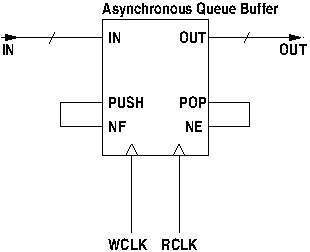
\includegraphics{sample}


            \subsection{SELECT}

                \subsubsection{purpose}

                    Select one of several inputs using CLB logic.

                \subsubsection{arguments}

                    \begin{tabular}{| l | l |}
                    \hline
                    Parameters  & unselected out - optional \\
                                & use alu - optional \\
                                & dsp - optional \\
                    \hline
                    Inputs      & select signal \\
                                & signal array \\
                                & select signal \\
                                & signal array \\
                                & . \\
                                & . \\
                                & . \\
                    \hline
                    Outputs     & signal array \\
                    \hline
                    \end{tabular}

                \subsubsection{description}

                    The inputs are in pairs. The first of each pair is an input
                    signal which selects the second of the pair (a signal array)
                    to be connected to the output signal array. The input arrays
                    may be smaller than the output array in which case
                    high-order input bits will padded or sign extended as
                    appropriate. If no select signals are high the output is
                    determined by hexadecimal string parameter {\bf unselected
                    out}, or is low if this parameter is not supplied.
                    Parameters {\bf use alu} and {\bf dsp} are flags used by the
                    platform-specific TDE list optimiser. Where an optional
                    parameter any leading parameters must be supplied.
                    
                    The selector may have duplicate inputs as these cannot
                    always be identified as the TDEVars may be connected together
                    later. Optimisation of duplicate inputs is resolved during
                    later netlist optimisation.

                \subsubsection{dump format}

                    \begin{lstlisting}[gobble=20, language=tde]
                        SELECT {
                            par: false
                            in:
                                S11
                                glob.a[0..7]
                                S15
                                glob.b[24..31]
                            out:
                                glob.c[0..7]
                        }
                    \end{lstlisting}

                \subsubsection{logic description}

                    Each output bit has an independent input selector. Where a
                    data input is narrower than the output, high order data bits
                    are connected to GND. These inputs will be optimised out during
                    low-level code generation. If a data input is wider than the
                    output the high order bits of the input will be ignored.

                    Xilinx target implementation -
                    
                    The logic depends on whether the default output is 0 or 1.
                    
                    for default 0 output -

                    A 1-input bit selector is implemented as an AND gate with 2
                    inputs, the data bit and the selector bit. When the selector
                    input is low, the output is low. When the selector input is
                    high the output is the same as the data input.

                    A 2-input selector is implemented using a 4-input LUT. Each
                    data input is ANDed with its selection input and the outputs
                    from these two ANDed inputs are ORed. 

                    Selectors with more than 2 inputs employ 4-input LUTs whose
                    outputs are ORed using the carry chain MUCYs. In that case
                    the LUT output is inverted.

                    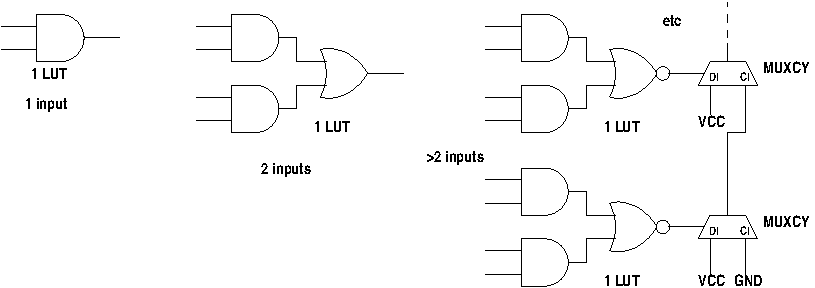
\includegraphics{select0}

                    for default 1 output -

                    A 1-input bit selector is implemented as an OR gate with 2
                    inputs, the data bit and the inverted selector bit. When the
                    selctor input is low the output is high. When the selector
                    bit is high is the same as the data input.

                    A 2-input selector is implemented using a 4-input LUT. Each
                    data input is ORed with its inverted selection input and the
                    outputs from these two ORed inputs are ANDed. 

                    Selectors with more than 2 inputs employ 4-input LUTs whose
                    outputs are ANDed using the carry chain MUCYs.

                    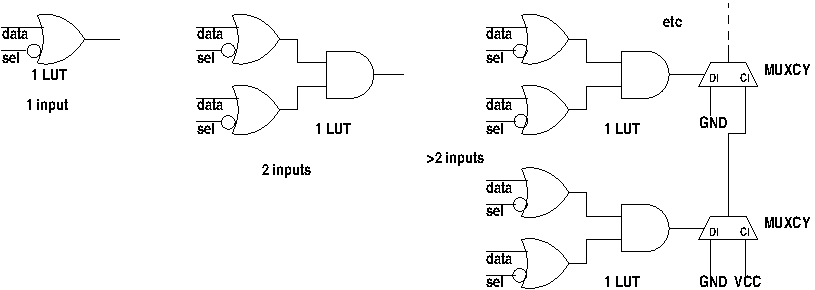
\includegraphics{select1}


            \subsection{SIG}

                \subsubsection{purpose}

                    Declare a signal or signal array.

                \subsubsection{arguments}

                    \begin{tabular}{| l | l |}
                    \hline
                    Parameters  & none \\
                    \hline
                    Inputs      & signal or signal array \\
                                & signal or signal array \\
                                & . \\
                                & . \\
                    \hline
                    Outputs     & none \\
                    \hline
                    \end{tabular}

                \subsubsection{description}

                    There may be any number of inputs. Each input
                    may be a single signal or an array. Declarations
                    are created which will be dimensioned if arrays.

                    This element is only used by the simulator, not the code
                    generator. It is not generated unless the -s or -T options
                    are passed to the compiler.

                \subsubsection{dump format}

                    \begin{lstlisting}[gobble=20, language=tde]
                        SIG     glob.a
                        SIG     E1[1]
                        SIG     S11
                        SIG     mod1_1.a[8]
                    \end{lstlisting}

                \subsubsection{logic description}

                    No logic is generated by this element.




%        \subsection{SIMREAD}
%
%            \subsubsection{purpose}
%            
%                Read a line from a file during simulation.
%
%            \subsubsection{arguments}
%            
%                \begin{tabular}{| l | l |}
%                \hline
%                Parameters  & string  file path name \\
%                \hline
%                Inputs      & clock signal \\
%                            & execution signal for the read \\
%                \hline
%                Outputs     & signal array driven from input data line \\
%                            & \ldots \\
%                            & \ldots \\
%                \hline
%                \end{tabular}
%
%            \subsubsection{description}
%
%                This element is only used by the simulator, not the code
%                generator. It is not generated unless the -s option
%                is passed to the compiler.
%                When the 2nd input signal is high, one line is read from the
%                file, is decoded according to the type of the output signal
%                arrays and the outputs are driven using the decoded values.
%                
%            
%            \subsubsection{dump format}
%            
%                This element is not printed.
%
%
%        \subsection{SIMWRITE}
%
%            \subsubsection{purpose}
%            
%                Write a line to a file during simulation.
%
%            \subsubsection{arguments}
%            
%                \begin{tabular}{| l | l |}
%                \hline
%                Parameters  & string  file path name \\
%                \hline
%                Inputs      & clock signal \\
%                            & execution signal for the write \\
%                            & signal array to be written to the data line \\
%                            & \ldots \\
%                            & \ldots \\
%                \hline
%                Outputs     & none \\
%                \hline
%                \end{tabular}
%
%            \subsubsection{description}
%
%                This element is only used by the simulator, not the code
%                generator. It is not generated unless the -s option
%                is passed to the compiler.
%                When the 2nd input signal is high, one line is written to the
%                file, each input signal array contributing one number to the
%                line.
%            
%            \subsubsection{dump format}
%            
%                This element is not printed.
%
%        \subsection{SIMVAR}
%
%            \subsubsection{purpose}
%            
%                A variable reference (only used by the simulator).
%
%            \subsubsection{arguments}
%            
%                \begin{tabular}{| l | l |}
%                \hline
%                Parameters  & Var class  variable \\
%                \hline
%                Inputs      & none \\
%                \hline
%                Outputs     & none \\
%                \hline
%                \end{tabular}
%
%            \subsubsection{description}
%
%                If the simulator is being used one of these elements is placed
%                on the list for every target variable.
%            
%            \subsubsection{dump format}
%            
%                This element is not printed.
%




        \subsection{SPECIAL}

            \subsubsection{purpose}
            
                Provides special functions, perhaps vendor specific.
                
            \subsubsection{arguments}
            
                \begin{tabular}{| l | l |}
                \hline
                Parameters  & Integer type of special function \\
                \hline
                Inputs      & \ldots \\
                \hline
                Outputs     & \ldots \\
                \hline
                \end{tabular}

            \subsubsection{description}

                 The first parameter is an integer type code which selects the
                 particular special function. At the moment there are only two
                 special functions.

                {\bf add line to the NCF or the XDC file}

                \begin{tabular}{| l | l |}
                \hline
                Parameters  & Integer 0 or 1 \\
                            & String  a format string \\
                \hline
                Inputs:     & signal  optional signal \\
                            & . \\
                            & . \\
                \hline
                Outputs:    & none \\
                \hline
                \end{tabular}

                The format string is written to the ISE NCF file or the Vivado
                XDC file. The format string may contain \%n or \%N conversions
                at which points netlist identifiers are to be inserted. The
                netlist identifiers are obtained from the input signals which
                are matched to the conversions in order. There will usually be
                only one of these though the format allows any number. \%n is
                replaced by the identifier of the next input signal argument.
                \%N is similar to the above but changes the identifier to upper
                case and removes any leading "GLOB\_" string. This is used for
                generating clock timing group names from the clock signal
                identifier. A \% followed by any other character is unchanged.
                The target mode signal arguments are matched to the \%n and \%N
                escape sequences left to right. The number of target mode
                arguments must must be suffient for the number of \%n and \%N
                escape sequences, any excess nets will being ignored.


            \subsection{START}

                \subsubsection{purpose}

                    Start an execution stream. There is one START for each
                    clock domain.

                \subsubsection{arguments}

                    \begin{tabular}{| l | l |}
                    \hline
                    Parameters  & none \\
                    \hline
                    Inputs      & start level signal \\
                                & clock signal \\
                    \hline
                    Outputs     & start pulse signal \\
                    \hline
                    \end{tabular}

                \subsubsection{description}

                    The start signal is a level. If there is
                    no explicit start level then this signal will be VCC.
                    
                    The clock signal is the clock for whose domain the start pulse
                    is being generated.
                    
                    When the start signal rises the rise is captured by the next
                    clock edge and an output pulse of one period duration is
                    generated on the next clock edge. The logic is locked after this
                    pulse so that any further start signal rises are ignored. The
                    start level is a global signal for all execution threads to
                    start. It must be re-synchronised to the clock domain to produce
                    a single start pulse to start all execution threads in the
                    domain. The start signal may be VCC if execution is to start
                    immediately after configuration loading, otherwise it must be
                    derived combinatorially from external inputs or from code
                    generated by inbuilt procedure start() whose code is outside
                    execution threads generated from 3PL source code.

                \subsubsection{dump format}

                    \begin{lstlisting}[gobble=20, language=tde]
                        START   glob.c100.start <- START=startsig, CLK=glob.c100
                    \end{lstlisting}

                \subsubsection{logic description}
                
                    If no start signal is supplied then a start pulse is
                    generated by a flip-flop whose D input is VCC. On the first
                    clock edge the output will go high. At the same time the
                    output of a second parallel flip-flop also goes high. This
                    is a lock signal to the reset of the first flip-flop which
                    on the next clock pulse will reset to low, the R input
                    having precedence over the D input. The output of the first
                    flip-flop will remain low as it is held reset.
                    
                    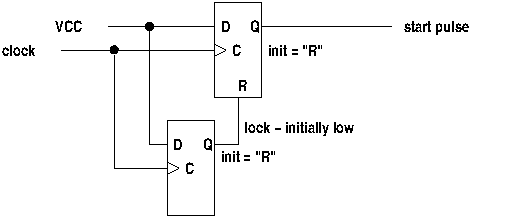
\includegraphics{starta}
                    
                    If a start signal is supplied the start logic differs only
                    in that the D inputs of two flip-flops are now driven by a
                    the start level via an intervening flip-flop. This
                    additional flip-flop is there to synchronise the
                    asynchronous start level transition to a clock edge. Timing
                    constrants will then ensure that paths to the following two
                    flip-flops will meet set and hold requirements.
                    
                    This form is not available for CPLDs.

                    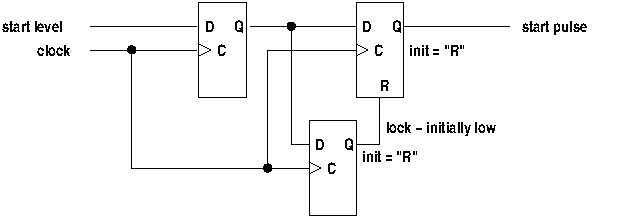
\includegraphics{starts}
                    
                    The output pulse from this element is distributed to all
                    ILOOP TDEs in the associated clock domain to start their
                    execution. To avoid problems with a posibly large fanout an
                    intervening single clock delay (DEL element, i.e. one DFF)
                    is inserted in each start path, a one-cycle delay
                    on startup not being significant.


            \subsection{TSELECT}

                \subsubsection{purpose}

                    Select one of several inputs using a 3-state driver.

                \subsubsection{arguments}

                    \begin{tabular}{| l | l |}
                    \hline
                    Parameters  & unselected out - optional \\
                    \hline
                    Inputs      & select signal \\
                                & signal array \\
                                & select signal \\
                                & signal array \\
                                & . \\
                                & . \\
                                & . \\
                    \hline
                    Outputs     & signal array \\
                    \hline
                    \end{tabular}

                \subsubsection{description}

                    The inputs are in pairs. The first of each pair is an input
                    signal which selects the second of the pair (a signal array)
                    to be connected to the output signal array. If no select
                    signals are high the output is determined by hexadecimal
                    string parameter {\bf unselected out}, or is low if this
                    parameter is not supplied. The input arrays may be smaller
                    than the output array in which case high-order input bits
                    will be connected low.
                    
                    

                \subsubsection{dump format}

                    \begin{lstlisting}[gobble=20, language=tde]
                        TSELECT {
                            par:
                            in:
                                S11
                                glob.a[0..7]
                                S15
                                glob.b[24..31]
                            out:
                                glob.c[0..7]
                        }
                    \end{lstlisting}

                \subsubsection{logic description}

                    Each output bit has a 3-state driver. Where a data input is
                    narrower than the output, high order data bits are connected
                    to GND. If a data input is wider than the output the high
                    order bits of the input will be ignored. The control input
                    is common to all outputs. Default output for each bit is
                    determined by a pullup or pulldown.

                    Xilinx target implementation -

                    A BUFE is used for each output bit. Default output must be
                    all 1s as pulldowns are not accepted. This TDE cannot be
                    used for FPGAs which do not have internal 3-state buffers,
                    e.g. Virtex-5 and later.


            \subsection{WAIT}

                \subsubsection{purpose}

                    A parallel block completion wait.

                \subsubsection{arguments}

                    \begin{tabular}{| l | l |}
                    \hline
                    Parameters  & none \\
                    \hline
                    Inputs      & clock signal \\
                                & reset signal or null \\
                                & input signal \\
                                & . \\
                                & . \\
                                & . \\
                    \hline
                    Outputs     & output signal \\
                    \hline
                    \end{tabular}

                \subsubsection{description}

                    There are four or more inputs. The first input signal is the
                    clock signal for the clock domain. The second input signal is a
                    reset signal or is null if there is no reset. The third and
                    following are finish signals. If all input signals go high
                    simultaneously the output signal also goes high, otherwise the
                    output signal goes high when the last input signal goes high.
                    The output signal is high for one clock cycle. The reset input
                    clears any pending latched completion signals.

                \subsubsection{dump format}

                    \begin{lstlisting}[gobble=20, language=tde]
                        WAIT {
                            in:
                                c100
                                null
                                S11
                                S13
                            out:
                                S15
                        }
                    \end{lstlisting}

                \subsubsection{logic description}

                    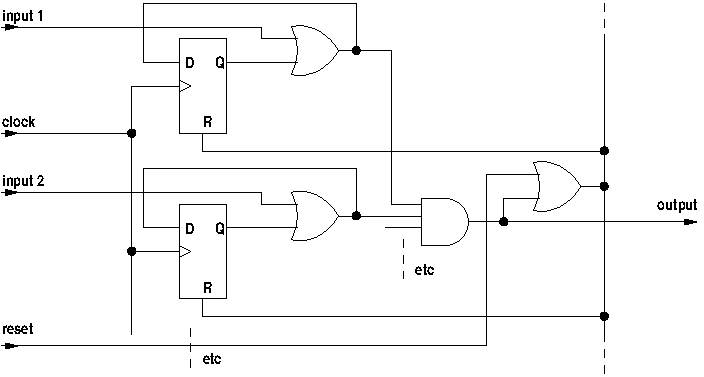
\includegraphics{wait}

                    If all WAIT inputs are high, all AND gate inputs are high (via
                    the OR gates) and hence the WAIT output is high. None of the
                    flip-flops are set because all resets are also driven high
                    via the WAIT output. If one or more inputs is low when an input
                    goes high the WAIT output will not go high and the
                    flip-flop associated with that input will be set. When the
                    last input finally goes high the previous latched inputs will be
                    ANDed with it, the WAIT output will go high and all latched
                    inputs will be reset. The reset input is ORed with the WAIT
                    output to reset all flip-flops.


            \subsection{WHEN}

                \subsubsection{purpose}

                    A {\em when} statement.

                \subsubsection{arguments}

                    \begin{tabular}{| l | l |}
                    \hline
                    Parameters  & none \\
                    \hline
                    Inputs      & start signal \\
                                & test signal \\
                                & true block finish signal or null \\
                                & false block finish signal or null \\
                    \hline
                    Outputs     & true block start signal \\
                                & false block start signal \\
                                & WHEN finish signal or null \\
                    \hline
                    \end{tabular}

                \subsubsection{description}

                    A start signal will be routed to either the true block start
                    output or the false block start output according to whether the
                    test input signal is high or low. The finish signals for the
                    true and false blocks are returned as inputs and the OR of these
                    emerges as the third output, signalling the end of the
                    statement.

                    A missing true or false block will have the block start signal
                    connected back to the associated block finish signal via a
                    1-cycle delay (TDEType.DEL). If both the true block and the
                    false block require a single DEL for their finish signals these
                    will be optimised to a separate common DEL from the start signal
                    to the finish signal. In that case -
                    \blist
                    \item   true block finish signal
                    \item   false block finish signal
                    \item   WHEN finish signal
                    \blend
                    arguments to the WHEN will all be null.

                \subsubsection{dump format}

                    \begin{lstlisting}[gobble=20, language=tde]
                        WHEN {
                            START           S22
                            TEST            glob.cpu_write_static_0.write_1[0]
                            T FINISH        TF24
                            F FINISH        FF27
                            T START         TS21
                            F START         FS22
                            FINISH          F30
                        }
                    \end{lstlisting}

                \subsubsection{logic description}

                    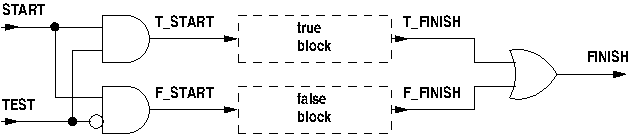
\includegraphics{whena}

                    The START signal is directed either through output T\_START or
                    F\_START depending on whether TEST is high or low. These
                    outputs execute either the true code block or the false code
                    block. The finish signals from the code blocks are ORed to get
                    the finish signal for the WHEN. If one of the code blocks is
                    missing a DEL will be inserted instead.

                    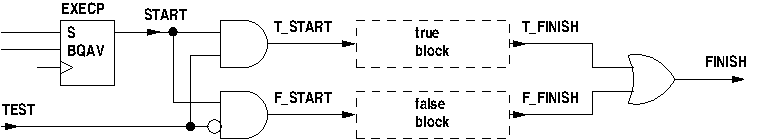
\includegraphics{whenb}

                    An EXECP is required at the START input if the test expression
                    contains queue reads. The BQAV input to the EXECP is the AND
                    of the .AV signals of all read queues in the test expression.


            \subsection{WHILE}

                \subsubsection{purpose}

                    A {\em while} statement.

                \subsubsection{arguments}

                    \begin{tabular}{| l | l |}
                    \hline
                    Parameters  & none \\
                    \hline
                    Inputs      & start signal \\
                                & test signal \\
                                & continuation signal from the body \\
                                & clock signal \\
                                & optional reset signal or null \\
                    \hline
                    Outputs     & start signal for the body \\
                                & WHILE finish signal \\
                    \hline
                    \end{tabular}

                \subsubsection{description}

                If the test input signal is high when start input signal goes high,
                the latter is routed to the body start output signal to execute the
                contained code block. If the test input signal is low when start
                input signal goes high, the latter is delayed by one clock cycle
                and then appears on the finish output signal (i.e. a {\em while}
                takes a minimum of one clock cycle). When the body code block
                finishes the last execution signal comes back to the continuation
                input signal. If the test input signal is high the continuation
                input signal is routed to the body start output signal to again
                execute the contained code block. If the test input signal is low
                the continuation input signal is routed through to the finish
                output signal, again with one clock cycle delay.

                The start signal and the continuation signal may come from
                EXECP elements which wait on queue availability in the test value.
                
                The optional reset signal clears internal state in the WHILE.

                \subsubsection{dump format}

                    \begin{lstlisting}[gobble=20, language=tde]
                        WHILE {
                            START_B     S22
                            FINISH      S30
                            <-
                            START       S24
                            TEST        E31[0]
                            CONTIN      S21
                            C           glob.c100
                            RESET       s34
                        }
                    \end{lstlisting}

                \subsubsection{logic description}

                    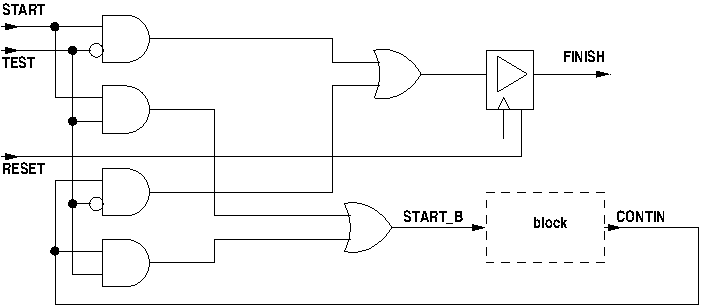
\includegraphics{whilea}

                    The WHILE samples the test expression value on initial entry
                    and on each subsequent iteration. If the test fails on initial
                    entry the START signal is routed through a DEL to FINISH. If
                    the test succeeds on initial entry START is passed on to the
                    code block via START\_B. When the code block finishes its
                    finish signal re-enters the WHILE logic via CONTIN where the
                    test value is again sampled. If the test succeeds the code
                    block is executed again. If the test fails CONTIN is directed
                    again through the DEL to FINISH. A RESET clears the DEL. The
                    DEL is required to avoid a race condition through to the
                    following statement.

                    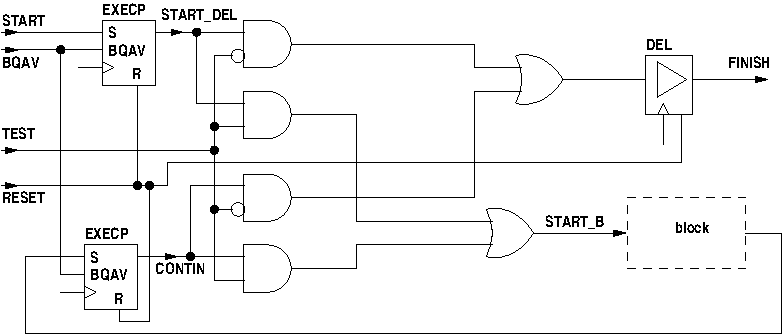
\includegraphics{whileb}

                    Two EXECPs are required if the test expression contains queue
                    reads. One controlling the START signal and the other
                    controlling the CONTIN signal. The BQAV input to both EXECPs is
                    the AND of the .AV signals of all read queues in the test
                    expression. A RESET clears the DEL and EXECPs.


            \subsection{XOR}

                \subsubsection{purpose}

                    An XOR gate for control signals.

                \subsubsection{arguments}

                    \begin{tabular}{| l | l |}
                    \hline
                    Parameters  & none \\
                    \hline
                    Inputs      & input signal \\
                                & input signal \\
                                & . \\
                                & . \\
                    \hline
                    Outputs     & AND signal \\
                    \hline
                    \end{tabular}

                \subsubsection{description}

                    Exclusive OR two or more input signals, the result appearing
                    on the output.

                \subsubsection{dump format}

                    \begin{lstlisting}[gobble=20, language=tde]
                        S11 = A12 ^ A14 ^ S8
                    \end{lstlisting}

                \subsubsection{logic description}

                    Xilinx implementation -

                    XOR gates with 1 to 4 inputs will be implemented in a
                    single LUT (single input gates will be eliminated during
                    low-level code generation). XOR gates with more than 4 inputs
                    generate nested XOR gates.








    \section{Intermediate code examples}

        Note that in the following examples the intermediate code dumps and the
        associated diagrams only show sections of the logic that illustrate the
        points under discussion - they are not complete listings or diagrams.
        
        In many cases clock inputs are not shown. The examples are constructed
        to use clock {\bf c100} and this can be assumed unless shown otherwise.
        
        In all the examples the signal {\bf glob.c100.start} appears. This is
        a single cycle pulse, synchronised to the {\bf c100} 100MHz clock, which
        is distributes to all execution threads to initiate them. In practice
        a recent change to the compiler has inserted a single cycle delay
        between this signal and every thread that it initiates but this is not
        shown in the examples. The purpose of the extra cycle is simply to avoid
        the path delays associated with distributing {\bf glob.c100.start} which
        can have a very high fanout. The inserted flip-flop in the path to each
        thread will be placed close the the logic that it initiates resulting
        in a much shorter path into the thread. {\bf glob.c100.start} will still
        have a high fanout but there is no combinatorial logic between its
        source and the myriad destination flip-flops.
    
        \subsection{top level sequential block}

            The code -
            \begin{lstlisting}[gobble=12, language=threepl]
                module "csiro/hymod/io1.3pl"

                useclock(c100);

                static({s1, s2}, "uint:8");

                seq {
                    s1 <- s2;
                    s2 <- s1;
                }
            \end{lstlisting}
            contains one execution thread. That thread will be an infinite loop
            containing two executable statements. The assignments do not wait on
            queues. The intermediate code would look like -
            \begin{lstlisting}[gobble=12, language=tde]
                startex = glob.startlevel_1[0]
                DEL F14 <- (1) glob.c100 S13
                DEL F17 <- (1) glob.c100 F14
                ILOOP       S13 <- glob.c100.start F17
                glob.startlevel_1[0] = VCC
                glob.startlevel_2[0] = VCC
                glob.startlevel[0] = glob.startlevel_2[0]
                START       glob.c100.start <- START=startex, CIN=glob.bus_clk, COUT=glob.c100
                glob.s1.CE[0..7] = S13
                glob.s1.D[0..7] = glob.s2[0..7]
                glob.s1.RES[0..7] = GND
                REG
                    OUT  glob.s1[0..7]
                    <-
                    CLK  glob.c100
                    DATA glob.s1.D[0..7]
                    CE   glob.s1.CE[0..7]
                    R    glob.s1.RES[0..7]
                    {0x00}
                glob.s2.CE[0..7] = F14
                glob.s2.D[0..7] = glob.s1[0..7]
                glob.s2.RES[0..7] = GND
                REG
                    OUT  glob.s2[0..7]
                    <-
                    CLK  glob.c100
                    DATA glob.s2.D[0..7]
                    CE   glob.s2.CE[0..7]
                    R    glob.s2.RES[0..7]
                    {0x00}
            \end{lstlisting}
            The multiple versions of value variable {\bf startlevel} (created
            in header code csiro/hymod/io1.3pl) are a result of the internal
            intricacies of the compiler. The last value the variable contains
            is assigned to the unappended identifier {\bf glob.startlevel}
            in an attempt to provide a useful value in simulation.

            Diagrammatically this is -

            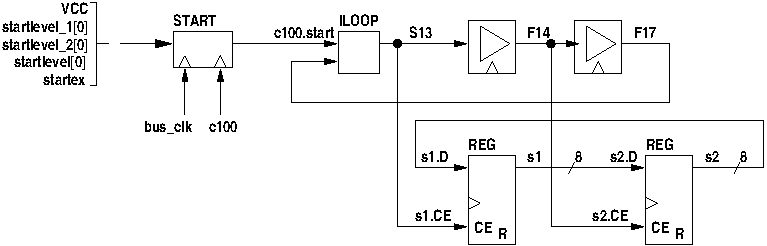
\includegraphics{e1}
            
            The thread is started from signal {\bf startex} which is connected to
            {\bf VCC}. This is sampled by {\bf bus\_clk} and then resynchronised to
            generate a single pulse using clock {\bf c100}. This is injected into
            {\bf ILOOP} to start the infinite loop. The execution signal for the
            body of the infinite loop is {\bf S13}. The loop body is a {\bf seq}
            block containing two statements. The first is executed by {\bf S13} and
            a finish signal is generated one clock cycle later ({\bf F14}. This
            finish signal is the start signal for the next statement. A finish
            signal is generated one clock cycle later for the second statement
            ({\bf F17}). This second finish signal marks the completion of the loop
            body code so it is fed back to the {\bf ILOOP} to generate the next
            iteration. There is no delay in {\bf ILOOP} (it is simply an OR gate)
            so the loop executes every two clock cycles.

            The two execute signals, {\bf S13} and {\bf F14} control the
            assignments to the two static variables {\bf s1} and {\bf s2} via their
            CE inputs.

        \subsection{top level static assignment}
        
            If we simplify the above code so that the infinite loop contains
            only a single assignment -
            \begin{lstlisting}[gobble=12, language=threepl]
                static({s1, s2}, "uint:8");

                s1 <- s2;
            \end{lstlisting}
            then the intermediate code is -
            \begin{lstlisting}[gobble=12, language=tde]
                startex = glob.startlevel_1[0]
                glob.startlevel_1[0] = VCC
                glob.startlevel_2[0] = VCC
                glob.startlevel[0] = glob.startlevel_2[0]
                START       glob.c100.start <- START=startex, CIN=glob.bus_clk, COUT=glob.c100
                glob.s1.CE[0..7] = S11
                glob.s1.D[0..7] = glob.s2[0..7]
                glob.s1.RES[0..7] = GND
                REG
                    OUT  glob.s1[0..7]
                    <-
                    CLK  glob.c100
                    DATA glob.s1.D[0..7]
                    CE   glob.s1.CE[0..7]
                    R    glob.s1.RES[0..7]
                    {0x00}
                glob.s2.RES[0..7] = GND
                REG
                    OUT  glob.s2[0..7]
                    <-
                    CLK  null
                    DATA null
                    CE   null
                    R    glob.s2.RES[0..7]
                    {0x00}  make const!
                DFF S11 <- C=glob.c100, S=glob.c100.start
            \end{lstlisting}
            which diagrammatically is -

            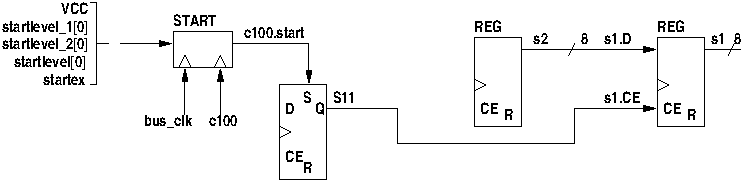
\includegraphics{e2}

            Since the {\bf ILOOP} contains a single statement which unconditionally
            takes one clock cycle, i.e. it executes on every clock cycle, the
            loop can be eliminated and instead the destination register clock
            enable can be asserted when execution starts and remain asserted
            from then on. This is done by a D-flip-flop which is set by the start
            signal. The output of the flip-flop provides an execute signal for
            every clock cycle.
            
            If the assignment is conditional -
            \begin{lstlisting}[gobble=12, language=threepl]
                static({s1, s2}, "uint:8");

                when (s1 != s2)
                    s1 <- s2;
            \end{lstlisting}
            then the intermediate code becomes -
            \begin{lstlisting}[gobble=12, language=tde]
                E8[0] = glob.s1[0..7] != glob.s2[0..7]      (uint, uint, log)
                WHEN {
                        START    SD7
                        TEST     E8[0]
                        T_FINISH null
                        F_FINISH null
                        T_START  S17
                        F_START  FS6
                        FINISH   null
                }
                glob._sdreset_1[0] = VCC
                glob._sdreset_2[0] = VCC
                START  glob.c100.start <- START=VCC, CIN=glob.c100, COUT=glob.c100
                glob._sdreset[0] = glob._sdreset_2[0]
                glob.s1.CE[0..7] = S17
                glob.s1.D[0..7] = glob.s2[0..7]
                glob.s1.RES[0..7] = GND
                REG
                    OUT  glob.s1[0..7]
                    <-
                    CLK  glob.c100
                    DATA glob.s1.D[0..7]
                    CE   glob.s1.CE[0..7]
                    R    glob.s1.RES[0..7]
                    {0x00}
                glob.s2.RES[0..7] = GND
                REG
                    OUT  glob.s2[0..7]
                    <-
                    CLK  null
                    DATA null
                    CE   null
                    R    glob.s2.RES[0..7]
                    {0x00}  make const!
                DFF SD7 <- C=glob.c100, S=glob.c100.start
            \end{lstlisting}

            Now the unoptimised logic for the above code would be -

            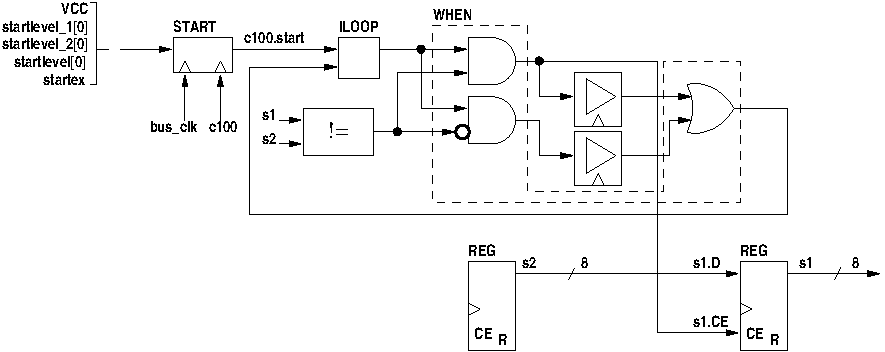
\includegraphics{e2cu}
            
            Since both the true and false bodies of the {\bf WHEN} execute
            in a single cycle (the unused false statement still requires a single
            cycle delay) this will be optimised to a single shared delay -

            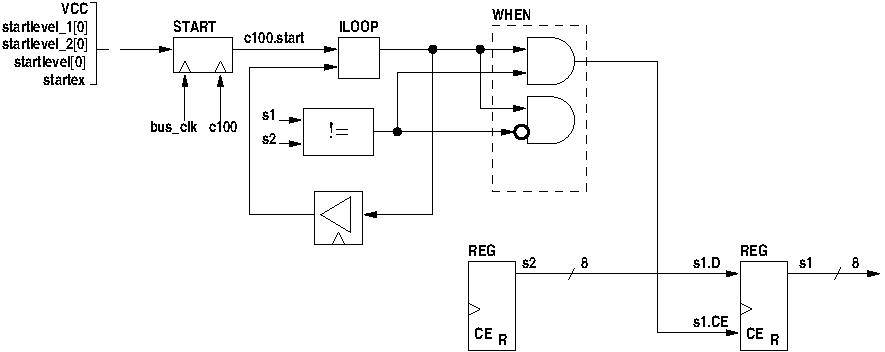
\includegraphics{e2cpo}
            
            The false side of the {\bf WHEN} is now unused so its AND gate will be
            omitted. The {\bf ILOOP} with a single delay feedback will be replaced
            with a set-once flip-flop -

            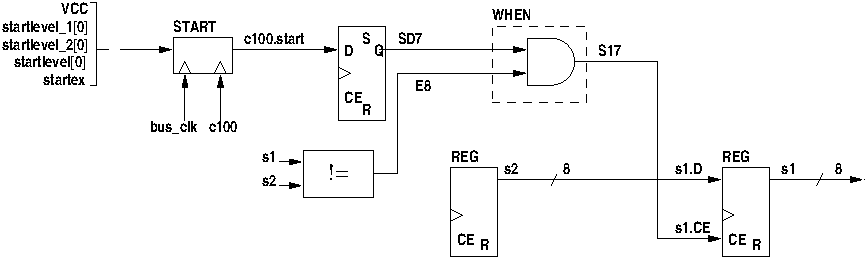
\includegraphics{e2o}
            
            Note that, like the simple assignment statement in the previous
            example, this logic has no execution thread any more. It is simply
            a register whose clock enable is asserted in clock cycles where the
            expression controlling the {\bf WHEN} is true.
            
            If the {\bf WHEN} false code block contained a single cycle statement
            rather than being omitted then the second AND gate would be retained
            but otherwise the logic would be the same.
            
            These examples show that top level assignments to static variables,
            even when conditional, have minimal logic overheads.

            
        \subsection{top level static assignment with queue reads}

            If the RHS of the assignment contains one or more queue reads then
            we must use an {\bf EXECP}. For example -

            \begin{lstlisting}[gobble=12, language=threepl]
                static(s, "uint:8");
                queue({p1, p2}, "uint:8");

                s <- p1 + p2;
            \end{lstlisting}
            the intermediate code is -
            \begin{lstlisting}[gobble=12, language=tde]
                startex = glob.startlevel_1[0]
                glob.startlevel_1[0] = VCC
                glob.startlevel_2[0] = VCC
                glob.startlevel[0] = glob.startlevel_2[0]
                START       glob.c100.start <- START=startex, CIN=glob.bus_clk, COUT=glob.c100
                E14[0..8] = glob.p1[0..7] + glob.p2[0..7]   (uint, uint, uint)
                S15[0..7] = cast(false){E14[0..8]}
                AV16 = AV18[0] AND AV19[0]
                ACK20[0] = S43
                ACK22[0] = S43
                EXECP       S43 <- C=glob.c100, EXEC=S11, AV16
                DEL F13 <- (1) glob.c100 S43
                ILOOP       S11 <- glob.c100.start F13
                glob.s.CE[0..7] = S43
                glob.s.D[0..7] = S15[0..7]
                glob.s.RES[0..7] = GND
                REG
                    OUT  glob.s[0..7]
                    <-
                    CLK  glob.c100
                    DATA glob.s.D[0..7]
                    CE   glob.s.CE[0..7]
                    R    glob.s.RES[0..7]
                    {0x00}
                glob.p1.RES = GND
                QUEUEBUFFER (2)
                    OUT    glob.p1[0..7]
                    NE     glob.p1.NE[0]
                    NF     glob.p1.NF[0]
                    CNT    null
                    SPC    null
                    WSTAT  null
                    RSTAT  null
                    <-
                    CLKOUT glob.c100
                    DATA   glob.p1.D[0..7]
                    PUSH   glob.p1.PUSH
                    POP    glob.p1.POP
                    R      glob.p1.RES
                glob.p1.POP = ACK22[0]
                AV19[0] = glob.p1.NE[0]
                glob.p2.RES = GND
                QUEUEBUFFER (2)
                    OUT    glob.p2[0..7]
                    NE     glob.p2.NE[0]
                    NF     glob.p2.NF[0]
                    CNT    null
                    SPC    null
                    WSTAT  null
                    RSTAT  null
                    <-
                    CLKOUT glob.c100
                    DATA   glob.p2.D[0..7]
                    PUSH   glob.p2.PUSH
                    POP    glob.p2.POP
                    R      glob.p2.RES
                glob.p2.POP = ACK20[0]
                AV18[0] = glob.p2.NE[0]
            \end{lstlisting}
            {\bf glob.p1.PUSH}, {\bf glob.p1.NF}, {\bf glob.p2.PUSH} and {\bf
            glob.p2.NF} are not connected here as they are used for assignments
            to the queues. Note that the code above would strictly give compiler
            errors since the queues have no sources (are not written). 
      
            The following shows the logic diagrammatically -

            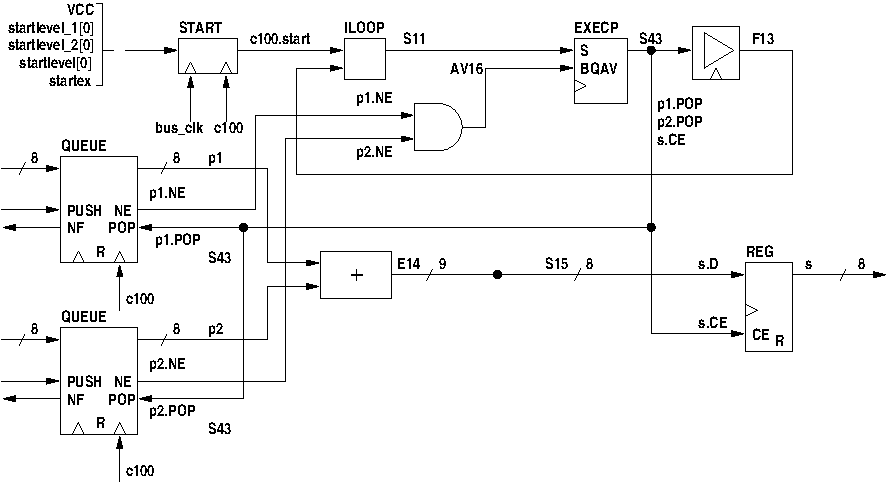
\includegraphics{e3}
            
            At the start {\bf c100.start} is a single cycle pulse which will be
            passed through {\bf ILOOP} to {\bf S11}. If {\bf AV16} is high (queues {\bf
            p1} and {\bf p2} are available for reading) then the pulse will
            in turn be passed as {\bf S43}, which executes the assignment to
            static {\bf s}. If {\bf AV16} is low the input pulse {\bf S11} is
            stored until {\bf AV16} goes high when {\bf S43} is finally driven
            by a single cycle pulse. The assignment executes in one cycle so a
            finish signal {\bf F13} is generated by a one cycle delay from {\bf
            S43}. The finish signal connects back to the {\bf ILOOP} to cause the next
            iteration. If {\bf AV16} remains high the assignment to {\bf s} will
            occur on every clock cycle, {\bf S11}, {\bf S43}, and {\bf F13}
            remaining high. {\bf S43} executes the assignment by raising the
            clock enable to static register {\bf s} ({\bf s.CE}). At the same
            time it pops queues {\bf p1} and {\bf p2} since {\bf p1.POP}
            and {\bf p2.POP} are connected to {\bf S43}. If either queue becomes
            unavailable for reading (empty) then {\bf p1.NE} or {\bf p2.NE} will
            go low and hence {\bf AV16} will go low, causing the {\bf EXECP} to wait.
            
            Note that the input to static register {\bf s} is 8 bits wide but
            the sum of the outputs of queues {\bf p1} and {\bf p2} is 9 bits
            wide. A cast() element from {\bf E14} to {\bf S15} will truncate
            the sum, ignoring the MSB.




        \subsection{top level queue assignment}
        
            If we change the above code to a queue assignment -

            \begin{lstlisting}[gobble=12, language=threepl]
                static(s, "uint:8");
                queue({p1, p2, p3}, "uint:8");

                p3 <<- p1 + p2;
            \end{lstlisting}
            the intermediate code is -
            \begin{lstlisting}[gobble=12, language=tde]
                E14[0..8] = glob.p1[0..7] + glob.p2[0..7]   (uint, uint, uint)
                S15[0..7] = cast(false){E14[0..8]}
                AV18[0] = glob.p2.NE[0]
                AV19[0] = glob.p1.NE[0]
                AV16 = glob.p3.NF[0] AND AV18[0] AND AV19[0]
                EXECP       SD24 <- C=glob.c100, EXEC=S11, AV16
                glob.p3.PUSH = SD24
                ACK20[0] = SD24
                glob.p2.POP = ACK20[0]
                ACK22[0] = SD24
                glob.p1.POP = ACK22[0]
                DEL F13 <- (1) glob.c100 SD24
                ILOOP       S11 <- glob.c100.start F13
                glob.p1.RES = GND
                QUEUEBUFFER (2)
                    OUT    glob.p1[0..7]
                    NE     glob.p1.NE[0]
                    NF     glob.p1.NF[0]
                    CNT    null
                    SPC    null
                    WSTAT  null
                    RSTAT  null
                    <-
                    CLKOUT glob.c100
                    DATA   glob.p1.D[0..7]
                    PUSH   glob.p1.PUSH
                    POP    glob.p1.POP
                    R      glob.p1.RES

                glob.p2.RES = GND
                QUEUEBUFFER (2)
                    OUT    glob.p2[0..7]
                    NE     glob.p2.NE[0]
                    NF     glob.p2.NF[0]
                    CNT    null
                    SPC    null
                    WSTAT  null
                    RSTAT  null
                    <-
                    CLKOUT glob.c100
                    DATA   glob.p2.D[0..7]
                    PUSH   glob.p2.PUSH
                    POP    glob.p2.POP
                    R      glob.p2.RES

                glob.p3.D[0..7] = S15[0..7]
                glob.p3.RES = GND
                QUEUEBUFFER (2)
                    OUT    glob.p3[0..7]
                    NE     glob.p3.NE[0]
                    NF     glob.p3.NF[0]
                    CNT    null
                    SPC    null
                    WSTAT  null
                    RSTAT  null
                    <-
                    CLKOUT glob.c100
                    DATA   glob.p3.D[0..7]
                    PUSH   glob.p3.PUSH
                    POP    glob.p3.POP
                    R      glob.p3.RES
            \end{lstlisting}

            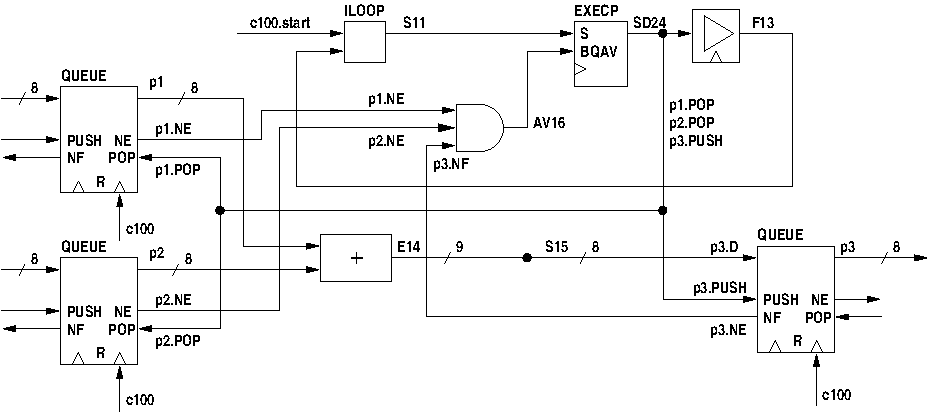
\includegraphics{e4}
            
            The assignment statement execution signal is now {\bf SD24}. The
            {\bf EXECP} now waits on {\bf p3.NF}, {\bf p1.NE} and {\bf p2.NE}. The
            assignment statement execution signal now drives {\bf p3.PUSH} to
            write to queue {\bf p3}.

        \subsection{multiple assignments to a variable}

            The following code has two threads, each an assignment to the same
            static variable {\bf s}. We assume here for the code to make sense
            that queues {\bf p1} and {\bf p2} are never available for reading
            simultaneously.
            \begin{lstlisting}[gobble=12, language=threepl]
                static(s, "uint:8");
                queue({p1, p2}, "uint:8");

                s <- p1;
                s <- p2;
            \end{lstlisting}
            the intermediate code is -
            \begin{lstlisting}[gobble=12, language=tde]
                AV16[0] = glob.p1.NE[0]
                AV14 = AV16[0]
                EXECP       S47 <- C=glob.c100, EXEC=S11, AV14
                ACK17[0] = S47
                glob.p1.POP = ACK17[0]
                DEL F13 <- (1) glob.c100 S47
                ILOOP       S11 <- glob.c100.start F13
                AV25[0] = glob.p2.NE[0]
                AV23 = AV25[0]
                EXECP       S48 <- C=glob.c100, EXEC=S20, AV23
                ACK26[0] = S48
                glob.p2.POP = ACK26[0]
                DEL F22 <- (1) glob.c100 S48
                ILOOP       S20 <- glob.c100.start F22
                S49 = S48 OR S47
                glob.s.CE[0..7] = S49
                SELECT {
                    in:
                        Var S47
                        Var glob.p1[0..7]
                        Var S48
                        Var glob.p2[0..7]
                    out:
                        Var glob.s.D[0..7]
                }
                glob.s.RES[0..7] = GND
                REG
                    OUT  glob.s[0..7]
                    <-
                    CLK  glob.c100
                    DATA glob.s.D[0..7]
                    CE   glob.s.CE[0..7]
                    R    glob.s.RES[0..7]
                    {0x00}
            \end{lstlisting}

            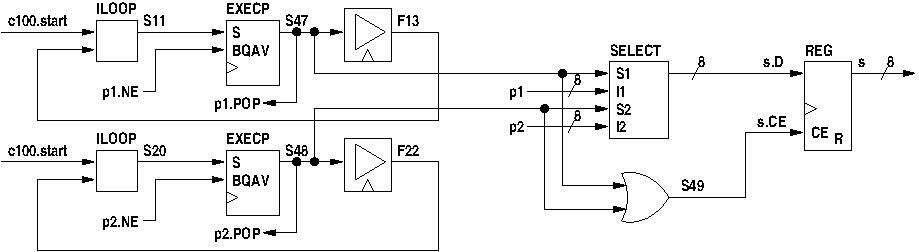
\includegraphics{e5}
            
            Each thread is an {\bf ILOOP} with an {\bf EXECP} to wait for queue availability
            and a 1-cycle delay. If the first assignment statement executes {\bf
            A18} goes high. If the second assignment statement executes {\bf
            S21} goes high. These are ORed to drive the clock enable of static
            variable {\bf s} to carry out the assignment. The input data source
            is selected by the {\bf SELECT} block with {\bf A18} or {\bf S21}
            selecting the appropriate data source (clearly it is a programming
            error if the assignments are not mutually exclusive).

        \subsection{general parallel block}
        
            A PAR block is implemented by using the same start signal for all
            statements in the block and waiting for all their finish signals
            using a WAIT element. For example the code -
            \begin{lstlisting}[gobble=12, language=threepl]
                static({s1, s2, s3}, "uint:8");

                par {
                    seq  {
                        s1 <- 3;
                        s2 <- 4;
                    }
                    s3 <- 5;
                }
            \end{lstlisting}
            generates the intermediate code -
            \begin{lstlisting}[gobble=12, language=tde]
                DEL S10 <- (1) glob.c100 S23
                DEL F11 <- (1) glob.c100 S10
                DEL F14 <- (1) glob.c100 S23
                WAIT {
                    in:
                        Var glob.c100
                        Var F11
                        Var F14
                    out:
                        Var F4
                }
                ILOOP       S23 <- glob.c100.start F4
            \end{lstlisting}

            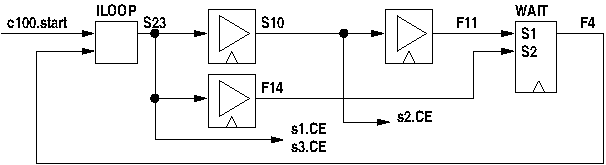
\includegraphics{e6}
            
            Execution signal {\bf S23} executes the assignments to {\bf s1} and
            {\bf s2} and Execution signal {\bf S10} executes the assignment to
            {\bf s3}.

        \subsection{minimal parallel block}
        
            If the statements in a PAR block all take one clock cycle and have
            no queue reads the compiler will eliminate parallel {\bf DEL} elements. For
            example the code -

            \begin{lstlisting}[gobble=12, language=threepl]
                static({s1, s2, s3}, "uint:8");

                par {
                    s1 <- 3;
                    s2 <- 4;
                    s3 <- 5;
                }
            \end{lstlisting}

            does not generate parallel delays, e.g. -

            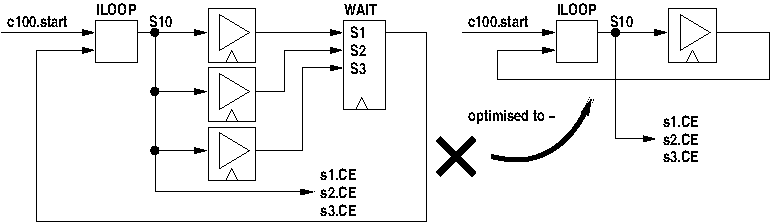
\includegraphics{e7}
            
            where {\bf S10} executes the three assignments.

        \subsection{general when statement}
        
            A {\bf WHEN} element directs an execution signal out through one of two
            outputs, the {\bf TRUE} output or the {\bf FALSE} output. These output
            signals execute the associated code block. The finish signals from the
            two code blocks must be ORed (they are mutually exclusive) to get the
            finish signal for the {\bf WHEN}. This {\bf OR} is contained in the {\bf
            WHEN} element. A missing code block is replaced by a single cycle
            delay, hence the minimum time to execute a {\bf WHEN} is one clock
            cycle. Note that if this minimum delay were not enforced we would have
            a combinatorial loop in this and other similar cases.     
            
            In the following example -
            \blist
            \item   the test contains queue reads
            \item   the FALSE block is missing
            \blend
            \vspace{5mm}

            \begin{lstlisting}[gobble=12, language=threepl]
                static(s, "uint:8");
                queue({p1, p2}, "uint:8");
                value(v, "uint:8", p1 + p2);

                when (v == 0)
                    s <- v;
            \end{lstlisting}

            the intermediate code is -

            \begin{lstlisting}[gobble=12, language=tde]
                E3[0..8] = glob.p1[0..7] + glob.p2[0..7]    (uint, uint, uint)
                S4[0..7] = cast(false){E3[0..8]}
                E10[0] = S4[0..7] == 0      (uint, uint, log)
                AV17[0] = glob.p1.NE[0]
                AV16[0] = glob.p2.NE[0]
                AV14 = AV16[0] AND AV17[0]
                ACK18[0] = A19
                ACK20[0] = A19
                EXECP       A19 <- C=glob.c100, EXEC=S11, AV14
                DEL F13 <- (1) glob.c100 A19
                DEL FF23 <- (1) glob.c100 FS8
                ACK24[0] = A25
                ACK26[0] = A25
                EXECP       A25 <- C=glob.c100, EXEC=S5, AV14
                WHEN {
                        START               A25
                        TEST                E10[0]
                        T FINISH    F13
                        F FINISH    FF23
                        T START             S11
                        F START             FS8
                        FINISH              F6
                }
                ILOOP       S5 <- glob.c100.start F6
                glob.s.CE[0..7] = A19
                glob.s.D[0..7] = S4[0..7]
                glob.s.RES[0..7] = GND
                REG
                    OUT  glob.s[0..7]
                    <-
                    CLK  glob.c100
                    DATA glob.s.D[0..7]
                    CE   glob.s.CE[0..7]
                    R    glob.s.RES[0..7]
                    {0x00}
                glob.v[0..7] = S4[0..7]
            \end{lstlisting}

            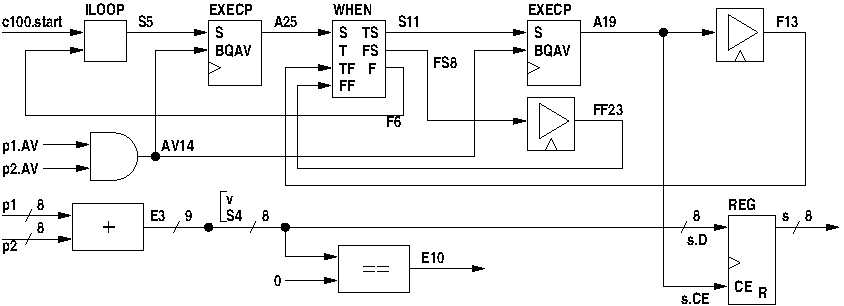
\includegraphics{e8}
            
            Note that there are two {\bf EXECP} elements, one to delay entry to the
            {\bf WHEN} element until queues {\bf p} and {\bf p2} are available for
            reading and the second to delay execution of the assignment inside
            the true block of the {\bf WHEN} until queues {\bf p} and {\bf p2} are
            available for reading. The inside {\bf EXECP} is redundant since on entry
            to the true block the availability of the two queues has already been
            verified by the first {\bf EXECP}. \footnote{The compiler should omit queue
            availability testing inside the {\bf WHEN} for queues already tested on
            entry to the {\bf WHEN}, but when expressions containing queue reads
            are complicated this turns out to be surprisingly difficult.} This
            inefficiency can be eliminated by enclosing the {\bf WHEN} by a SYNC
            element which will eliminate both {\bf EXECP}s and replace them with a
            single {\bf EXECP} before the {\bf WHEN} (where the first one is now).
            
            Note also that there is no false code block so a single cycle delay
            is used instead ({\bf FS8} to {\bf FF23}).
            

        \subsection{minimal when statement}
        
            The compiler recognises the special case where both the true and
            false code blocks execute in a single cycle, i.e. have a single {\bf DEL}
            element. This also applies where a parallel block executes in one
            cycle and all the {\bf DEL} elements are collapsed to a single {\bf DEL} as
            described previously. Single {\bf DEL} blocks for the true and false
            blocks can be replaced by a single {\bf DEL} block from the start signal
            to the {\bf WHEN}. As an example the following code -
            \begin{lstlisting}[gobble=12, language=threepl]
                static({s1, s2}, "uint:8");
                static(l, "log");

                seq {
                    nop();
                    when (l) par{
                        s1 <- 3;
                        s2 <- 4;
                    }
            }
            \end{lstlisting}
            
            results in the intermediate code -
            \begin{lstlisting}[gobble=12, language=tde]
                DEL S5 <- (1) glob.c100 S4
                DEL F7 <- (1) glob.c100 S5
                WHEN {
                        START               S5
                        TEST                glob.l[0]
                        T_FINISH    null
                        F_FINISH    null
                        T_START             S16
                        F START             FS9
                        FINISH              null
                }
                ILOOP       S4 <- glob.c100.start F7
            \end{lstlisting}

            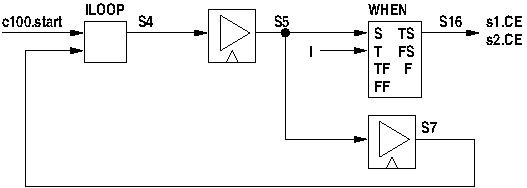
\includegraphics{e9a}
            
            Notes -
            \blist
            \item   the false start signal {\bf FS9} goes nowhere
            \item   the nop() generates the first {\bf DEL} and has been included
                    simply to stop the logic collapsing even further to a single
                    D-flip-flop set by {\bf c100.start} - see below
            \item   {\bf S16} is the execution signal for both assignments in
                    the true code block of the {\bf WHEN}
            \blend
            
            To expand on the comment about the nop(), if we simplify the code to
            -
            \begin{lstlisting}[gobble=12, language=threepl]
                static({s1, s2}, "uint:8");
                static(l, "log");

                when (l) par{
                    s1 <- 3;
                    s2 <- 4;
                }
            \end{lstlisting}
            the intermediate code becomes -
            \begin{lstlisting}[gobble=12, language=tde]
                WHEN {
                        START               SD7
                        TEST                glob.l[0]
                        T FINISH    null
                        F FINISH    null
                        T START             S23
                        F START             FS6
                        FINISH              null
                }
                DFF SD7 <- C=glob.c100, S=glob.c100.start
            \end{lstlisting}

            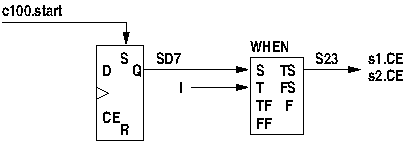
\includegraphics{e9b}

            The {\bf ILOOP} and any {\bf DEL}s have disappeared. {\bf SD7} goes high after
            {\bf c100.start} and remains high thereafter. {\bf s23} goes high
            whenever the {\bf WHEN} test is true and causes the two assignments to
            occur.
            

        \subsection{simple target while statement}
        
            The following example is a target while statement where the loop
            test does not contain queue reads -
            \begin{lstlisting}[gobble=12, language=threepl]
                static({s1, s2}, "uint:8");
                static(l, "log");

                seq while (l) {
                    s1 <- 5;
                    s2 <- 6;
                }
            \end{lstlisting}
            
            the intermediate code is -

            \begin{lstlisting}[gobble=12, language=tde]
                DEL S10 <- (1) glob.c100 SB4
                DEL CD13 <- (1) glob.c100 S10
                WHILE {
                        START_B         SB4
                        FINISH          F14
                        <-
                        START       SD12
                        TEST                glob.l[0]
                        CONTIN      CD13
                        C               glob.c100
                }
                ILOOP       SD12 <- glob.c100.start F14
            \end{lstlisting}

            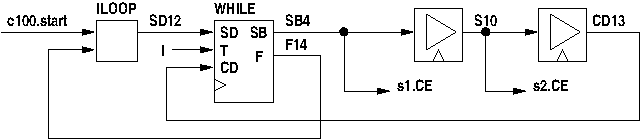
\includegraphics{e10}
            
            The {\bf WHILE} element has two entry points, {\bf START\_DEL} is the
            initial entry point and {\bf CONTIN\_DEL} is the entry point for
            further iterations. {\bf START\_B} is the start signal for the
            contained code block and {\bf FINISH} is the finish signal from the
            {\bf WHILE}.
            
            The signal {\bf SB4} executes the first assignment statement and
            {\bf S10} executes the second. The loop takes two clock cycles per
            iteration with no extra overheads, but if on initial entry the
            test is false the {\bf WHILE} has an internal delay of one clock cycle
            between the start input ({\bf SD12} into F) and the finish signal
            ({\bf F14} at F). This ensures that the {\bf WHILE} takes a minimum of
            one clock cycle.
            

        \subsection{target while statement with queue waits}
        
            If the {\bf WHILE} test expression contains queue reads an {\bf EXECP} appears in
            both the START\_DEL and CONTIN\_DEL inputs. If the loop body
            contains queue reads then {\bf EXECP} elements will appear there as well.
            The following example has both.
            \begin{lstlisting}[gobble=12, language=threepl]
                static(s, "uint:8");
                queue({p1, p2, p3, p4, p5, p6}, "uint:8");
                static(l, "log");

                par while (p1 || p2) {
                    s <- p3;
                    p4 <<- p5 + p6;
                }
            \end{lstlisting}
            
            The intermediate code is -

            \begin{lstlisting}[gobble=12, language=tde]
                E5[0] = glob.p1[0] OR glob.p2[0]
                AV13[0] = glob.p3.NE[0]
                AV11 = AV13[0]
                EXECP       S89 <- C=glob.c100, EXEC=SB4, AV11
                ACK14[0] = S89
                glob.p3.POP = ACK14[0]
                DEL F10 <- (1) glob.c100 S89
                E20[0..8] = glob.p5[0..7] + glob.p6[0..7]   (uint, uint, uint)
                S21[0..7] = cast(false){E20[0..8]}
                AV24[0] = glob.p5.NE[0]
                AV25[0] = glob.p6.NE[0]
                AV22 = glob.p4.NF[0] AND AV24[0] AND AV25[0]
                EXECP       S93 <- C=glob.c100, EXEC=SB4, AV22
                ACK26[0] = S93
                ACK28[0] = S93
                glob.p5.POP = ACK26[0]
                glob.p6.POP = ACK28[0]
                DEL F19 <- (1) glob.c100 S93
                WAIT {
                    in:
                        Var glob.c100
                        Var F10
                        Var F19
                    out:
                        Var F7
                }
                WHILE {
                        START_B             SB4
                        FINISH              F33
                        <-
                        START       SD31
                        TEST                E5[0]
                        CONTIN      CD32
                        C               glob.c100
                }
                ACK38[0] = SB4
                ACK40[0] = SB4
                glob.p2.POP = ACK38[0]
                glob.p1.POP = ACK40[0]
                AV37[0] = glob.p1.NE[0]
                AV36[0] = glob.p2.NE[0]
                AV34 = AV36[0] AND AV37[0]
                EXECP       SD31 <- C=glob.c100, EXEC=S3, AV34
                EXECP       CD32 <- C=glob.c100, EXEC=F7, AV34
                ILOOP       S3 <- glob.c100.start F33
            \end{lstlisting}

            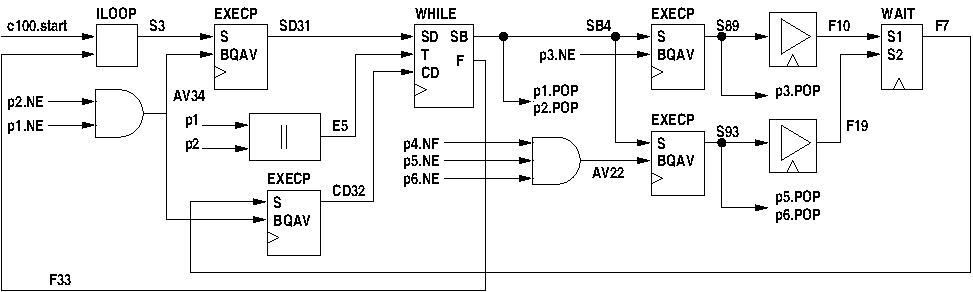
\includegraphics{e11}
            
            The variables have not been shown.
            {\bf S89} is the execution signal for the static assignment and
            {\bf S93} is the execution signal for the queue assignment.
            

        \subsection{simple target do-while statement}
        
            The following code illustrates a target {\bf DO\_WHILE} loop with no queue
            dependencies -
            \begin{lstlisting}[gobble=12, language=threepl]
                static({s1, s2}, "uint:8");
                static(l, "log");

                par do {
                    s1 <- 4;
                    s2 <- 5;
                } while (l);
            \end{lstlisting}
            
            The intermediate code is -

            \begin{lstlisting}[gobble=12, language=tde]
                DEL FD5 <- (1) glob.c100 SB4
                DO WHILE {
                        START_B                     SB4
                        FINISH                      F6
                        <-
                        START                   S3
                        TEST                    glob.l[0]
                        FINISH_B_DEL    FD5
                }
                ILOOP       S3 <- glob.c100.start F6
            \end{lstlisting}

            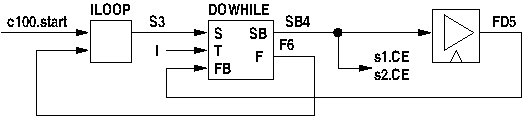
\includegraphics{e12}
            
            Note that since the two parallel assignment statements take a single
            cycle a single delay element is used to time them and single signal
            {\bf SB4} executes both. No parallel {\bf WAIT} is necessary.

        \subsection{target do-while statement with queue waits}

            If we take the above example and introduce queue dependencies in both
            the test expression and one of the body statements -
            \begin{lstlisting}[gobble=12, language=threepl]
                static(s, "uint:8");
                queue(p1, "log");
                queue({p2, p3}, "uint:8");

                par do {
                    s <- 4;
                    p2 <<- p3;
                } while (p1);
            \end{lstlisting}
            
            the intermediate code is -

            \begin{lstlisting}[gobble=12, language=tde]
                    AV17[0] = glob.p3.NE[0]
                    AV15 = glob.p2.NF[0] AND AV17[0]
                    EXECP       S56 <- C=glob.c100, EXEC=SB4, AV15
                    ACK18[0] = S56
                    glob.p3.POP = ACK18[0]
                    glob.p2.PUSH = S56
                    DEL F8 <- (1) glob.c100 S56
                    AV23[0] = glob.p1.NE[0]
                    AV21 = AV23[0]
                    EXECP       SD26 <- C=glob.c100, EXEC=F8, AV21
                    DO WHILE {
                            START_B         SB4
                            FINISH          F6
                            <-
                            START                   S3
                            TEST                    glob.p1[0]
                            FINISH_B_DEL    SD26
                    }
                    ACK24[0] = SD26
                    glob.p1.POP = ACK24[0]
                    glob.s.CE[0..7] = SB4
                    ILOOP       S3 <- glob.c100.start F6
            \end{lstlisting}

            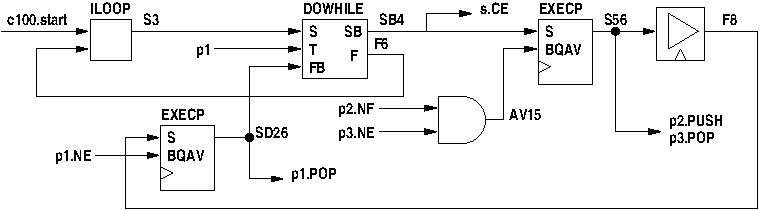
\includegraphics{e13}
            
            The parallel body of the loop has one assignment with queue dependencies
            and one without. The latter takes a fixed single cycle so it is
            executed using the block execute signal {\bf SB4} whereas the queue
            assignment has an {\bf EXECP} before being executed by {\bf S56}. Since
            the queue assignment will take at least one cycle the delay for the
            static assignment and the parallel {\bf WAIT} have been omitted by the
            compiler.

            Note that the {\bf FINISH\_BLOCK} input to the {\bf DO\_WHILE} is via
            an {\bf EXECP} since the block iteration test contains a queue read.

        \subsection{multiple queue reads within a module}
        
            Multiple queue reads read the same datum if simultaneous or
            separate data otherwise. The queue pops are ORed. The
            following code illustrates this -
            \begin{lstlisting}[gobble=12, language=threepl]
                queue({p1, p2, p3}, "uint:8");

                p2 <<- p1;
                p3 <<- p1;
            \end{lstlisting}
            
            The intermediate code is -

            \begin{lstlisting}[gobble=12, language=tde]
                AV8[0] = glob.p1.NE[0]
                AV6 = glob.p2.NF[0] AND AV8[0]
                EXECP       S51 <- C=glob.c100, EXEC=S3, AV6
                ACK9[0] = S51
                DEL F5 <- (1) glob.c100 S51
                ILOOP       S3 <- glob.c100.start F5
                AV15 = glob.p3.NF[0] AND AV8[0]
                EXECP       S52 <- C=glob.c100, EXEC=S12, AV15
                ACK17[0] = S52
                DEL F14 <- (1) glob.c100 S52
                ILOOP       S12 <- glob.c100.start F14
                glob.p1.POP = ACK17[0] OR ACK9[0]
                glob.p2.D[0..7] = glob.p1[0..7]
                glob.p2.PUSH = S51
                glob.p3.D[0..7] = glob.p1[0..7]
                glob.p3.PUSH = S52
            \end{lstlisting}

            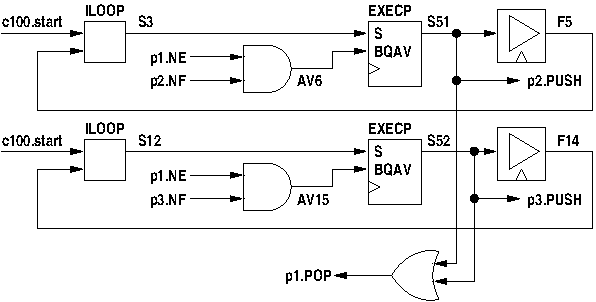
\includegraphics{e14}
            

        \subsection{multiple queue reads in different modules}
        
            Where multiple queue reads are in different modules each
            module must execute a read before the queue is poped,
            this occurring simultaneously with the last read. Multiple
            reads within a module are again ORed.
            \begin{lstlisting}[gobble=12, language=threepl]
                queue({p1, p2, p3, p4}, "uint:8");

                [
                    p2 <<- p1;
                    p3 <<- p1;
                ]
                p4 <<- p1;
            \end{lstlisting}

            Note that the first two assignments are in an inline module and the
            third assignment is in the file module. The intermediate code is -

            \begin{lstlisting}[gobble=12, language=tde]
                AV6 = glob.p2.NF[0] AND AV8[0]
                ACK9[0] = S71
                EXECP       S71 <- C=glob.c100, EXEC=S3, AV6
                DEL F5 <- (1) glob.c100 S71
                ILOOP       S3 <- glob.c100.start F5
                AV15 = glob.p3.NF[0] AND AV8[0]
                ACK17[0] = S72
                EXECP       S72 <- C=glob.c100, EXEC=S12, AV15
                DEL F14 <- (1) glob.c100 S72
                ILOOP       S12 <- glob.c100.start F14
                AV23 = glob.p4.NF[0] AND AV25[0]
                ACK26[0] = S73
                EXECP       S73 <- C=glob.c100, EXEC=S20, AV23
                DEL F22 <- (1) glob.c100 S73
                ILOOP       S20 <- glob.c100.start F22
                S69 = ACK26[0]
                S70 = ACK17[0] OR ACK9[0]
                DIVERGE {
                    in:
                        Var glob.c100
                        Var glob.p1.RES
                        Var glob.p1.NE[0]
                        Var S69
                        Var S70
                    out:
                        Var glob.p1.POP
                        Var AV25[0]
                        Var AV8[0]
                }
                glob.p1.RES = GND
                glob.p2.D[0..7] = glob.p1[0..7]
                glob.p2.PUSH = S71
                glob.p3.D[0..7] = glob.p1[0..7]
                glob.p3.PUSH = S72
                glob.p4.D[0..7] = glob.p1[0..7]
                glob.p4.PUSH = S73
            \end{lstlisting}

            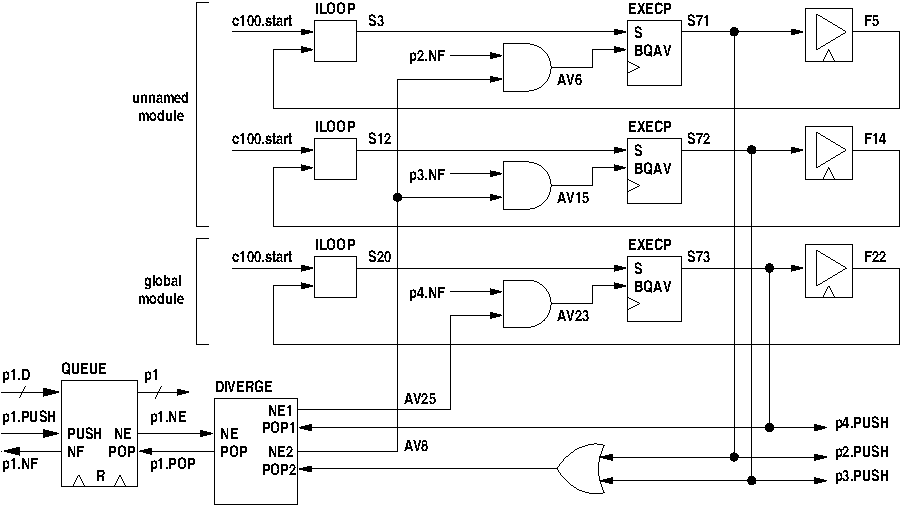
\includegraphics{e15}


        \subsection{multiple queue writes}
        
            Multiple writes to queues are treated independently regardless of which
            module they are in. The writes are simply {\bf OR}ed and the code must
            be constructed such that conflicts do not occur (there are no
            compile-time or run-time checks).

            \begin{lstlisting}[gobble=12, language=threepl]
                queue({p1, p2, p3}, "uint:8");

                p1 <<- p2;
                p1 <<- p3;
            \end{lstlisting}
            
            The intermediate code is -

            \begin{lstlisting}[gobble=12, language=tde]
                AV8[0] = glob.p2.NE[0]
                AV6 = glob.p1.NF[0] AND AV8[0]
                EXECP       S48 <- C=glob.c100, EXEC=S3, AV6
                ACK9[0] = S48
                glob.p2.POP = ACK9[0]
                DEL F5 <- (1) glob.c100 S48
                ILOOP       S3 <- glob.c100.start F5
                AV17[0] = glob.p3.NE[0]
                AV15 = glob.p1.NF[0] AND AV17[0]
                EXECP       S49 <- C=glob.c100, EXEC=S12, AV15
                ACK18[0] = S49
                glob.p3.POP = ACK18[0]
                DEL F14 <- (1) glob.c100 S49
                ILOOP       S12 <- glob.c100.start F14
                S50 = S49 OR S48
                glob.p1.PUSH = S50
                SELECT {
                    in:
                        Var S48
                        Var glob.p2[0..7]
                        Var S49
                        Var glob.p3[0..7]
                    out:
                        Var glob.p1.D[0..7]
                }
            \end{lstlisting}

            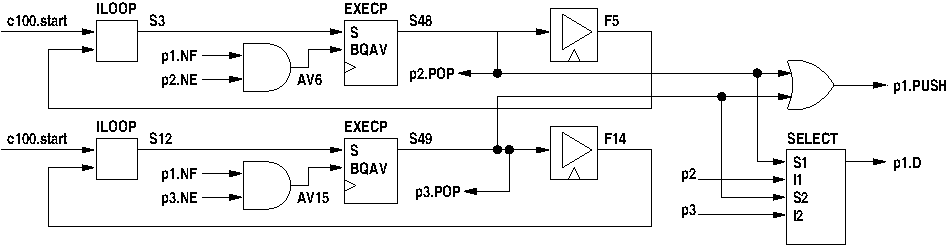
\includegraphics{e16}


        \subsection{unbuffered queue reads and writes}\label{ubqueuerw}

            An unbuffered queue is used to synchronise two execution threads. In some
            texts this is referred to as a rendezvous. One thread reads the queue
            (uses its value) and the other thread writes to the queue (assigns to
            it). The first thread to reach the queue read/write will wait until the
            other thread also reaches the complementary write/read then they will
            both execute their respective statements and a datum will be transferred
            (if the type is not "null"). An unbuffered queue is only available for
            reading when a write is pending. Similarly it is only available for
            writing when a read is pending. Unbuffered queue read availability ({\bf
            RAV} output) is high when the {\bf WRITE} input is high. Similarly write
            availability({\bf WAV} output) is high when the {\bf READ} input is high.
            Thus each thread accessing the queue must wait on availability and at the
            same time assert the {\bf WRITE} or {\bf READ} as required. A normal
            queue has {\bf PUSH} or {\bf POP} asserted by the {\bf START\_DEL} output
            of an EXECP when {\bf BQAV} is high. An unbuffered queue {\bf WRITE} or
            {\bf READ} must assert the {\bf WRITE} or {\bf READ} ahead of execution
            when any/all buffered queues involved are available and the write or read
            is pending.            
            
            Thus for unbuffered queues reads and writes the {\bf WPENDING} output of
            an EXECP is used to drive the {\bf WRITE} and the {\bf RPENDING} output
            the {\bf READ} inputs to the queue buffer rather than using the {\bf
            START\_DEL} outputs (the label QUEUEBUFFER is a misnomer here as the
            queue is unbuffered, however for convenience it is regarded as a variant
            of the same element). The unbuffered queue contains no internal logic
            other than the cross conenctions from {\bf WRITE} to {\bf RAV},
            {\bf READ} to {\bf WAV} and from data input to data output.
            
            As an example consider the following three assignment statements executing
            in separate threads -
            
            \begin{lstlisting}[gobble=12, language=threepl]
                s <- ubq1;
                .
                .
                ubq1 <<- ubq2;
                .
                .
                ubq2 <<- n;
            \end{lstlisting}
            
            where {\bf ubq1} and {\bf ubq2} are unbuffered queues and {\bf n} and
            {\bf s} do not involve queues.

            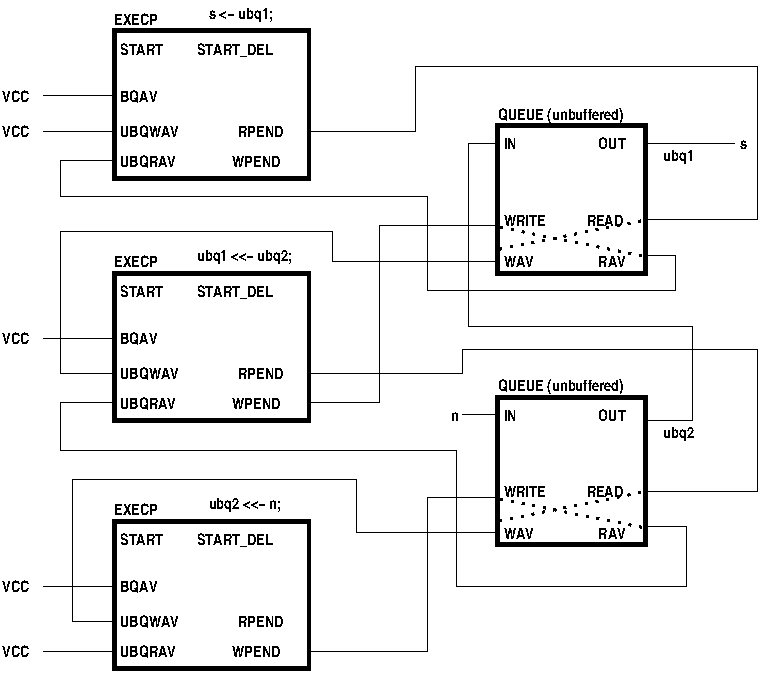
\includegraphics{ubqueueex1}
            
            The three assignments do not contain buffered queue references so the
            {\bf BQAV} inputs to the EXECPs are VCC>

            The first assignment does not assign to an unbuffered queue so the {\bf
            UBQWAV} input is VCC. When execution reaches this statement the {\bf
            RPEND} will be asserted since {\bf UBQWAV} is high. This will flow into
            the {\bf READ} input and out of the {\bf WAV} output of {\bf ubq1} to the
            {\bf UBQWAV} input of the 2nd EXECP.

            When execution reaches the second assignment the high {\bf UBQWAV} will
            result in {\bf RPEND} being asserted which will in turn flow through the
            {\bf READ} and {\bf WAV} ports of {\bf ubq2} to the {\bf UBQWAV} input of
            the last EXECP.

            Similarly when execution reaches the third assignment the high {\bf
            UBQRAV} will flow back through {\bf ubq2}, the 2nd EXECP and {\bf ubq1}
            to the {\bf UBQRAV} input of the first EXECP.

            Thus when all three assignment statements are ready to execute all three
            EXECPs will have {\bf BQAV}, {\bf UBQWAV} and {\bf UBQRAV} high and can
            thus execute simultaneously (in one clock cycle), transfering the value
            of {\bf n} through to {\bf s} in the process.
            
            The following is a simplified diagram of the write chain from the above
            example -
            
            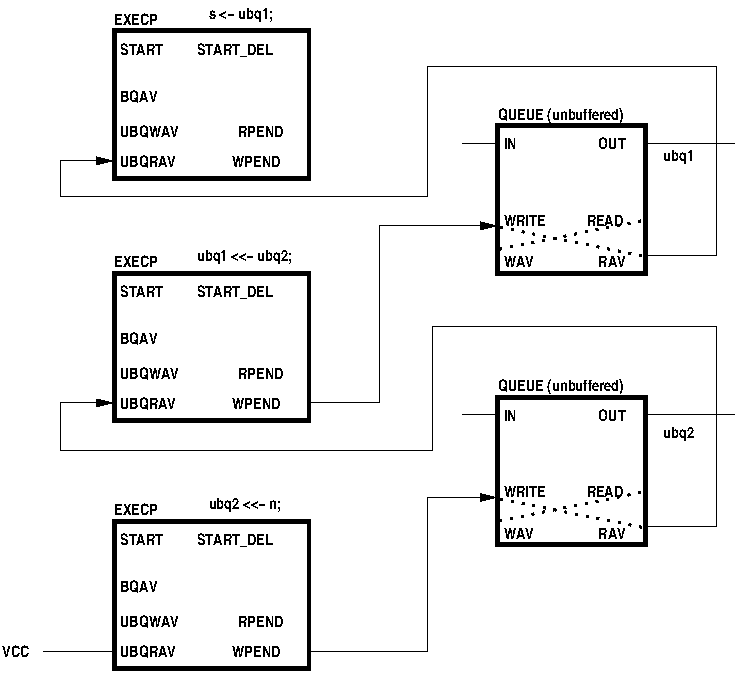
\includegraphics{ubqueueex1_wchain}
            
            The chain starts at the bottom left with VCC for UBQRAV since that
            assignment statement RHS does not contain an unbuffered queue.
            
            Note that read availability anywhere along the chain will be true when
            all upstream assigment EXECPs have received a start signal in their
            respective execution streams and any associated buffered queues are
            availabile for reading or writing as appropriate.
            
            The other half of the signalling, the read chain, is shown in the
            following diagram.
            
            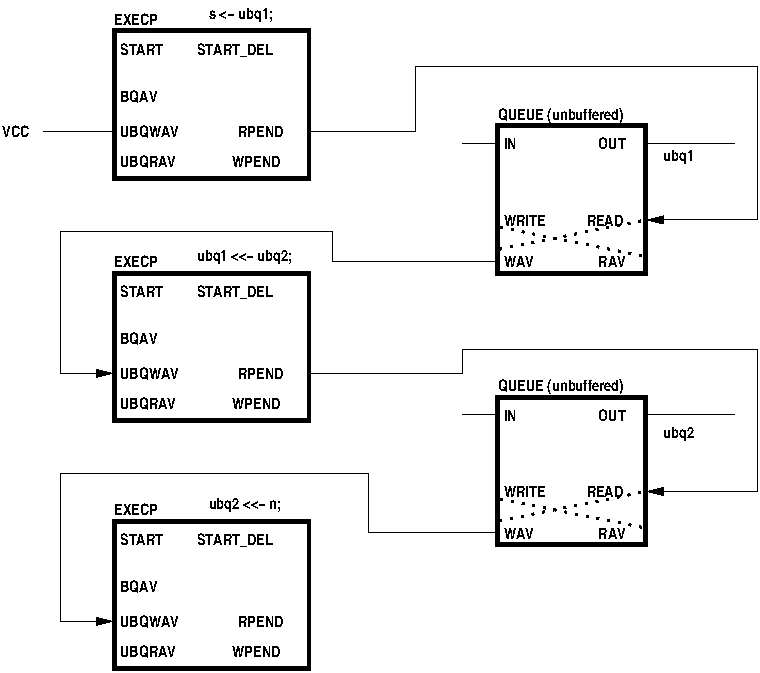
\includegraphics{ubqueueex1_rchain}
            
            The chain starts at the top right with VCC for UBQWAV since that
            assignment statement LHS does not contain an unbuffered queue.
            
            In a similar manner to the write chain write availability anywhere along
            the chain will be true when all downstream stream assigment EXECPs have
            received a start signal in their respective execution streams and any
            associated buffered queues are availabile for reading or writing as
            appropriate.
            
            
            
            Since the pending outputs of EXECPs are only asserted if the {\bf BQAV}
            input is high assignments containing both buffered queues and unbuffered
            queues will wait until any buffered queues are available to be read or
            written as appropriate.
                        
            Note that the availability of a buffered queue can be asserted and then
            de-asserted due to simultaneous queue operations by unrelated threads.
            This is not a problem as the availability of all buffered and
            unbuffered queues referenced by an assignment statement is assessed
            on a per-cycle basis.
            
            Assignment statements containing unbuffered queues may contain mutiple
            queues of both types.
            
            Buffered and unbuffered queues may be read or written in multiple places
            however simultaneous writes must be avoided, either by the inherent logic
            of the program or else explicitly by use of waitprilock statements.
            Simultaneous reads of unbuffered queues are valid, however unbuffered
            queue reads take no account of the modules in which they occur, all reads
            being independent.
                        
            Multiple {\bf WRITE} and {\bf READ} signals to an
            unbuffered queue are ORed to each input and responses are orchestrated by
            any EXECP elements involving those queues. The following example
            expands the previous example by including multiple unbuffered queue
            reads and writes -
            
            \begin{lstlisting}[gobble=12, language=threepl]
                s <- ubq1;
                .
                .
                ubq1 <<- ubq2;
                .
                .
                ubq2 <<- n;
                .
                .
                s <- ubq2;
                .
                .
                ubq2 <<- ubq1;
                .
                .
                ubq1 <<- n;
            \end{lstlisting}
            
            Note that this example is intended to show logic generated for multiple
            unbuffered queue reads and writes and does not necessarily make
            any sense!
            
            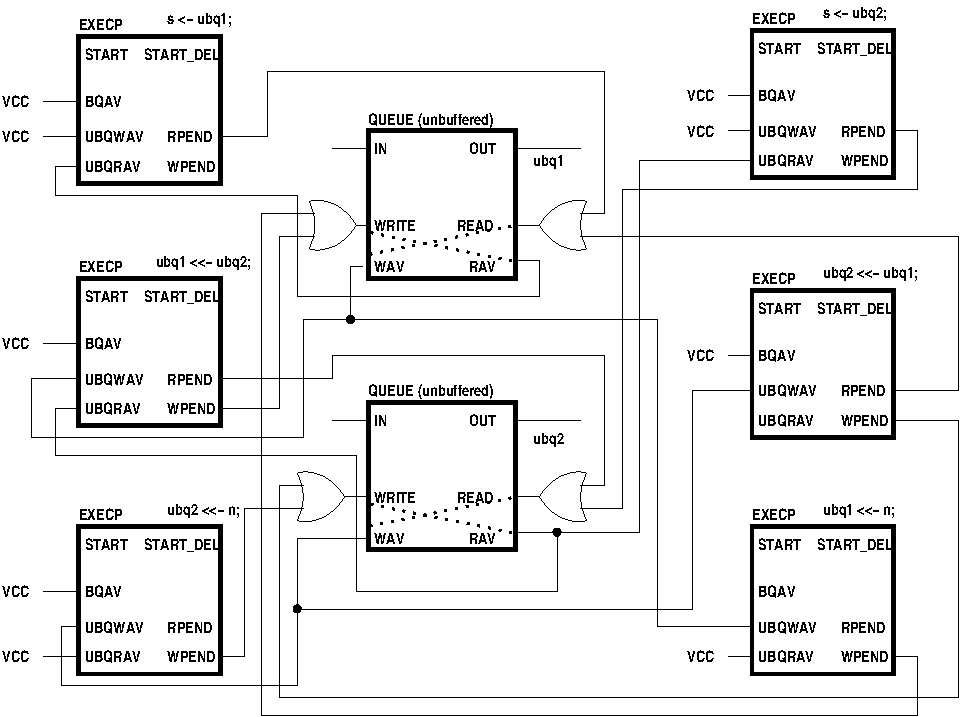
\includegraphics{ubqueueex2}


        \subsection{"unless" constructs}
        
            The {\bf unless} construct is implemented using ordinary intermediate
            code elements. The code follows one of two patterns -
            \blist
            \item   the exception expression contains no queue reads
            \item   the exception expression does contain queue reads
            \blend
            If an exception code block is present then that is spliced
            into the execution logic. A flip-flop is added the block
            which is subject to the {\bf unless} construct to register
            whether execution is taking place within the subject block.
            If the subject block does not have any executing statements within
            it then the exception is ignored.
            
            If the exception expression contains no queue reads, a {\bf WHEN} is
            used to detect the exception. The value of the exception expression is
            {\bf AND}ed with the subject execution flip-flop to form the test input
            to the {\bf WHEN}. The output of the {\bf WHEN} resets all {\bf DEL},
            {\bf WAIT}, {\bf EXECP} and {\bf WHILE} elements in the subject killing
            all execution. A second {\bf WHEN} then loops through a {\bf DEL}
            waiting for the exception experssion to go false. The false output of
            the second {\bf WHEN} then drives the finish of an enclosing {\bf
            ILOOP} driving the first {\bf WHEN}.
            
            If the exception expression contains queue reads, the first {\bf WHEN}
            is preceded by an {\bf EXECP} and the second {\bf WHEN} is not needed as
            a queue read is a single event, not a duration.
            
            In either case the finish signal is {\bf OR}ed with the finish signal of the
            subject block so that it appears to complete.

            An exception code block is spliced in after the {\bf WHEN} and prior to
            the finish signal.

            The following example, {\bf ee1.3pl}, illustrates the case where the
            exception expression contains no queue reads -

            \begin{lstlisting}[gobble=12, language=threepl]
                module "csiro/hymod/io2.3pl"

                useclock(c100);

                static({e, l}, "log");
                static({v1, v2, v3}, "uint:8");

                when (l) {
                    seq {
                        v1 <- 3;
                        par {
                            v2 <- 5;
                            v3 <- 7;
                        }
                    }
                } unless (e) {
                    seq {
                        v1 <- 0;
                        v2 <- 0;
                    }
                }
            \end{lstlisting}
            
            The intermediate code for the control logic for the {\bf WHEN} is -

            \begin{lstlisting}[gobble=12, language=tde]
                ILOOP  S74 <- SSD114 OR113
                OR113 = F75 OR RS101
                WHEN {
                        T_START  S79
                        F_START  FS77
                        FINISH   F75
                        <-
                        START    S74
                        TEST     ee1.l[0]
                        T_FINISH F86
                        F_FINISH FF95
                }
                DEL  S92 <- (1) glob.c166 S79 TS73
                DEL  F86 <- (1) glob.c166 S92 TS73
                DEL  FF95 <- (1) glob.c166 FS77 TS73
                OR98 = F75 OR TS73
                DFF {
                        OUT      FDRS99
                        <-
                        D        -
                        C        glob.c166
                        CE       -
                        R        OR98
                        S        S74
                }
                .
                .
                ee1.v1.CE[0..7] = S79
                .
                .
                ee1.v2.CE[0..7] = S92
                .
                .
                ee1.v3.CE[0..7] = S92
            \end{lstlisting}
            
            In diagramatic form this is -

            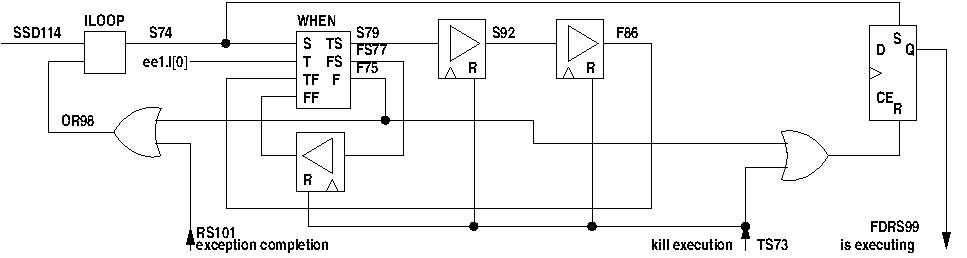
\includegraphics{ee1a}
            
            Note that there is no parallel wait - the optimiser has noted that the
            two assignments in parallel take exactly one clock cycle and has
            replaced two {\bf DEL}s and a {\bf WAIT} with one {\bf DEL} ({\bf S92}
            to {\bf F86}). The first {\bf DEL} in the {\bf SEQ}, {\bf S79} to {\bf
            S92} is for the first assignment, hence v1.CE is driven by {\bf S79}.
            The two parallel assignments, {\bf v2.CE} and {\bf v3.CE}, are driven by
            {\bf S92}. {\bf F86} completes the true block of the {\bf WHEN} and
            feeds back to the true finish input to emerge as the finish output for
            the {\bf WHEN}, {\bf F75}.

            If there were no {\bf UNLESS} construct the flip-flop and three gates
            would be omitted, {\bf F75} connecting back to the {\bf ILOOP}.

            The OR gate between {\bf F75} and the {\bf ILOOP} is to allow an
            execution pulse to be injected as an alternative finish signal for the
            {\bf WHEN} after execution of the {\bf WHEN} has been killed. {\bf
            RS101} is the new execution completion pulse.

            Execution of the {\bf WHEN} is killed by resetting all control logic
            state within it, in this case just the three {\bf DEL}s. The kill signal
            is {\bf TS73}.

            The exception logic needs to know if the {\bf WHEN} is actually
            executing (it may be nested inside other constructs and not actually be
            executing at the moment - in this example it is always executing since
            it is at the top level, hence the {\bf ILOOP}). The flip-flop is set
            when the {\bf WHEN} begins execution and is reset when the {\bf WHEN}
            finishes or execution is killed by {\bf TS73}. If the false branch of
            the {\bf WHEN} is taken there is a single {\bf DEL} in the {\bf ILOOP}
            and hence the {\bf WHEN} executes on every cycle.
            
            The intermediate code for the exception control logic is -

            \begin{lstlisting}[gobble=12, language=tde]
                ILOOP  S102 <- SSD100 S103
                AND106[0] = ee1.e[0] AND FDRS99
                WHEN {
	                T_START  TS73
	                F_START  FS107
	                FINISH   S103
	                <-
	                START    S102
	                TEST     AND106[0]
	                T_FINISH RS101
	                F_FINISH FF108
                }
                DEL  S64 <- (1) glob.c166 TS73
                DEL  S68 <- (1) glob.c166 S64
                DEL  F70 <- (1) glob.c166 S68
                DEL  FF108 <- (1) glob.c166 FS107
                OR112 = F70 OR S111
                WHEN {
	                T_START  TS110
	                F_START  RS101
	                FINISH   -
	                <-
	                START    OR112
	                TEST     ee1.e[0]
	                T_FINISH -
	                F_FINISH -
                }
                DEL  S111 <- (1) glob.c166 TS110
                .
                .
                ee1.v1.RES[0..7] = S64
                .
                .
                ee1.v2.RES[0..7] = S68
            \end{lstlisting}
            
            In diagramatic form this is -

            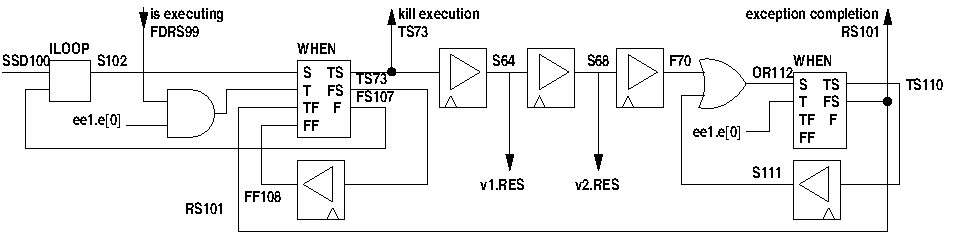
\includegraphics{ee1b}
            
            This logic runs independently in its own {\bf ILOOP}. The first {\bf
            WHEN} waits for the exception expression ({\bf ee1.l[0]}) to be
            asserted, but only if the associated subject construct is executing
            ({\bf FDRS99}). When this is not true, the execution emerges on the
            false output, {\bf FS107}, through a {\bf DEL} to the false finish {\bf
            FF108} and then emerges from the when finish output as {\bf S103} and
            feeds back to the {\bf ILOOP} for the next clock cycle. Thus the {\bf
            WHEN} tests every clock cycle. When the exception occurs the true output
            of the {\bf WHEN} is asserted. This is {\bf TS73} which kills all
            execution in the associated subject code. Execution proceeds through
            three {\bf DEL}s executing the {\bf SEQ} in the exception code block. If
            there was no exception code block there would be a single {\bf DEL}
            here. Progressive stages, {\bf S64} and {\bf S68}, reset variables {\bf
            v1} and {\bf v2} in the {\bf SEQ} block. At the completion of the
            exception code block a second {\bf WHEN} waits for the exception
            expression to go false, the true branch output looping back via a {\bf
            DEL} and the OR gate. When ee1.e[0] goes false, the execution signal
            emerges on the true branch of the {\bf WHEN}, {\bf RS101}, which
            completes execution of the killed subject block. It also feeds back to
            the true finish input of the first when, emerging as the finish signal,
            {\bf S103}, feeding back to the enclosing {\bf ILOOP} to wait for the
            next exception.

            If the exception expression contains queue reads a single {\bf WHEN}
            combined with an {\bf EXECP} is used, for example {\bf ee2.3pl} -

            \begin{lstlisting}[gobble=12, language=threepl]
                module "csiro/hymod/io1.3pl"

                useclock(c166);

                static(l, "log");
                queue(e, "log");
                static({v1, v2, v3}, "uint:8");

                when (l) {
                    seq {
                        v1 <- 3;
                        par {
                            v2 <- 5;
                            v3 <- 7;
                        }
                    }
                } unless (e) {
                    seq {
                        v1 <- 0;
                        v2 <- 0;
                    }
                }
            \end{lstlisting}
            
            The intermediate code for the exception control logic containing
            a queue read is -

            \begin{lstlisting}[gobble=12, language=tde]
                ILOOP  S102 <- SSD100 S103
                EXECP {
	                START_DEL SD113
	                PRI_IN    -
	                PENDING   P112
	                <-
	                CLK       glob.c166
	                START_IN  S102
	                BQAV       ee2.e.NE
                        UBQAV     -
	                PRI_OUT   -
	                RESET     -
                }
                AND106[0] = ee2.e[0] AND FDRS99
                WHEN {
	                T_START  TS73
	                F_START  FS107
	                FINISH   S103
	                <-
	                START    SD113
	                TEST     AND106[0]
	                T_FINISH RS101
	                F_FINISH FF108
                }
                DEL  S64 <- (1) glob.c166 TS73
                DEL  S68 <- (1) glob.c166 S64
                DEL  RS101 <- (1) glob.c166 S68
                DEL  FF108 <- (1) glob.c166 FS107
                .
                .
                ee2.v1.RES[0..7] = S64
                .
                .
                ee2.v2.RES[0..7] = S68
            \end{lstlisting}
            
            In diagramatic form this is -

            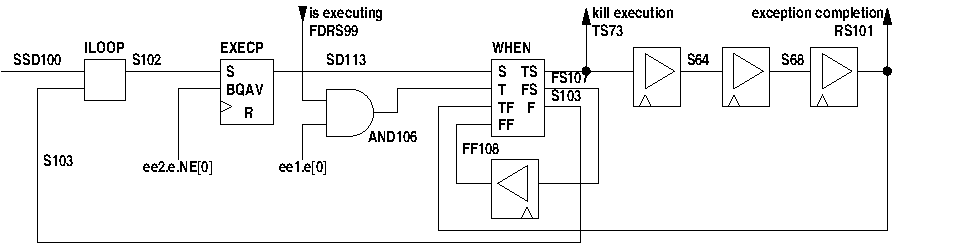
\includegraphics{ee2b}
            
            The exception logic now waits for queue {\bf e} to be not empty.
            Execution is then passed to the {\bf WHEN}. If the value is false, the
            {\bf WHEN} loops back to the {\bf ILOOP} via a {\bf DEL} and {\bf
            FF108}, emerging from the {\bf WHEN} on the finish output {\bf S103}.

            If the exception value is true subject execution is killed and the
            execution signal goes through three {\bf DEL}s as before. On emerging ({\bf
            RS101}) it completes execution of the subject block and loops back to the
            true completion input of the {\bf WHEN}, emerging as the {\bf WHEN}
            finish signal {\bf S103}, completing the {\bf ILOOP}.




\chapter{Writing inbuilt modules, procedures and functions}\label{inbuilt}
        
    

    The following illustrates the class definition for an inbuilt function,
    in this case {\bf sin()} -
    
    \begin{lstlisting}[gobble=4, language=java]
        package threepl.funcs;

        import threepl.exceptions.ExEx;
        import threepl.exec.Val;
        import threepl.nodes.NodeList;
        import threepl.parser.Constant;
        import threepl.parser.SrcLoc;

        /**
         * An inbuilt function to get the sine.
         */
        public class SinFunc extends InbuiltFunc implements Constant {
            .
            .
            .
        }
    \end{lstlisting}

    For inbuilt modules and procedures the class definition is similar to that
    for functions -
        
    \begin{lstlisting}[gobble=4, language=java]
        package threepl.procs;

        import threepl.exceptions.ExEx;
        import threepl.exec.Ref;
        import threepl.exec.Val;
        import threepl.nodes.NodeList;
        import threepl.parser.Constant;
        import threepl.parser.SrcLoc;
        import threepl.parser.Functions;


        /**
         * An inbuilt procedure to scan a string converting delimited fields to types specified
         * by a format string.
         */
        public class SscanfProc extends InbuiltProc implements Constant {
            .
            .
            .
        }
    \end{lstlisting}
    
    For procedures there is an optional constructor, e.g. -
    
    \begin{lstlisting}[gobble=4, language=java]
        public SscanfProc () {
            allowed_as_param = false;
            check_null_input_args = true;
            check_null_output_args = true;
            target_inline = false;
        }
    \end{lstlisting}
    
    These boolean variables are all declared and initialised in
    InbuiltProc.java and their functions are as follows -
    
    \blist
    \item allowed\_as\_param - true if the procedure is allowed as a
        parameter-creation procedure, i.e. can appear as a parameter in
        a function module or procedure definition.
    \item check\_null\_input\_args - if true null input arguments will throw
        an exception
    \item check\_null\_output\_args - if true null output arguments will throw
        an exception
    \item target\_inline - if true the procedure generates in-line target code
    \blend
    
    These booleans are set false by the super class but assigning them here
    improves readability. The null argument detection avoids the need in many
    cases for the module or procedure to explicitly check if an argument is null.
    Some procedures however accept null arguments and hence do not want this test
    enabled.
    
    There are two additional member variables, applicable to both modules
    and procedures -
    
    \begin{lstlisting}[gobble=4, language=java]
        public TreeMap<String,Integer>  ipnames;
        public TreeMap<String,Integer>  opnames;
    \end{lstlisting}
    
    which are null by default. These maps can contain identifiers to be
    associated with the module or procedure input and output parameters so that
    the module or procedure can be passed arguments either by position or by
    parameter=argument. If these maps are null then only the usual 
    parameter/argument association by position is available. The map keys contain
    the parameter identifiers and the associated integers are the parameter
    position. The maps need not contain all parameters as it is often convenient
    to pass some initial mandatory arguments by position.
    
    When a parameter name map has been provided the parameter=name arguments
    will be re-arranged in the argument list so that the module or
    procedure only sees arguments in the correct order. Note that for many
    modules and procedures null arguments are allowed in the call and in addition
    the argument re-arrangement for parameter=argument entries may also
    introduce null arguments.
    
    Inbuilt modules, procedures and functions are listed in maps in
    InbuiltMods.java, InbuiltProcs.java and InbuiltFuncs.java e.g. -
    
    \begin{lstlisting}[gobble=4, language=java]
        public InbuiltProcs () {
            procs = new TreeMap<String, InbuiltProc>();

            procs.put("addmodeattribute", new AddModeAttributeProc());
            .
            .
            .
        }
    \end{lstlisting}
    
    Here the map key is the identifier by which the module, procedure
    or function is called and the associated entry is the actual
    module, procedure or function. The identifiers are lower case
    and the actual classes are camel case with "Mod", "Proc" or "Func"
    appended, but this is only a convention.    

    The calling procedure for inbuilt modules, procedures and functions
    is the same with the exception that functions do not have output
    parameters.
    
    Functions have a getVal() method to return the function value.
    For example the {\bf sin()} function -
    
    \begin{lstlisting}[gobble=4, language=java]
        public Val getVal (NodeList args) {
            SrcLoc  loc = args.getCallLoc();

            if (args.size() != 1)
                throw new ExEx("sin() - must have one argument", loc);
            .
            .
            .
    \end{lstlisting}
    
    class {\bf NodeList} is a linked list of nodes in the compiled code
    tree. Variable {\bf args} contains the list of arguments of the
    function call.
    
    Class {\bf SrcLoc} contains source code file name, line number and
    character column. {\bf doc} is assigned the function call location.
    
    The size of {\bf args} is checked to ensure that the number of arguments
    provided is correct.
    
    Modules and procedures have an execute() method.
    For example the procedure {\bf sscanf()} -
    
    \begin{lstlisting}[gobble=4, language=java]
        public void execute (
            NodeList    inargs, 
            NodeList    outargs, 
            boolean     toplevel
    ) {
        SrcLoc      loc = inargs.getCallLoc();
        if (inargs.size() != 2)
            throw new ExEx("sscanf() must have two input arguments", loc);
        if (outargs.size() == 0)
            throw new ExEx("sscanf() must have one or more output arguments", loc);        
        .
        .
        .
    \end{lstlisting}
    
    The signature is similar for a module except that the {\bf toplevel}
    parameter is not present.
    
    Where a procedure is allowed to be called to create a parameter in a
    module, procedure or function definition the call to the procedure
    is more complicated, e.g. for inbuilt procedure {\bf int()} -
       
    \begin{lstlisting}[gobble=4, language=java]
        public IntProc () {
            allowed_as_param = true;
            check_null_input_args = true;
            check_null_output_args = false;
            target_inline = false;
            allowed_attributes = true;
        }

        /**
         * Execute the variable declaration procedure int().
         */
        public ArrayList<Var> execute (
            NodeList            inargs,
            NodeList            outargs,
            ArrayList<String>   names,
            RefOrVal            par_arg,
            int[]               dim_des,
            boolean             is_input,
            boolean             is_output
        ) {
            .
            .
            .
        }
    \end{lstlisting}
    
    The extra member variable {\bf allowed\_attributes} is true to indicate that
    the arguments to the procedure can contain attributes. Attributes are passed
    as attribute=value. Some must be processed by the module or procedure itself.
    In the case of procedures {\bf clock()}, {\bf input()} and {\bf output()}
    attributes are processed by 3PL code whenever the procedure is called via a
    3PL call-back procedure. If this variable is true then a mixture of
    parameter=argument and attribute=value arguments will be resolved. Arguments
    to the module or procedure will appear in the argument list as simple
    positional arguments as a result of the identifier resolution described
    above. Any that are not recognised are assumned to be attribute=value and
    these will be appended as additionak arguments following the positional
    arguments and will be class KeyMatchNode. These trailing attributes must be
    processed by the module or procedure.
    
    The arguments to execute() are -
      
    \blist
    \item inargs is a list of input argument tree nodes
    \item outargs is a list of output argument tree nodes
    \item names is a list of identifiers evaluated via method
            getIdents() prior to calling execute()
    \item par\_arg is an argument passed to this variable as a parameter in
            a call
    \item dim\_des is a dimensional description for a compound constant
            argument or is null - it must be null here!
    \item is\_input is true if this variable is the input parameter
            for a module, procedure or function
    \item is\_output is true if this variable is the output parameter
            for a module or procedure 
    \blend
    
    The procedure must return an ArrayList<Var> containing the variable(s).

    The call arguments are supplied separately by {\bf inargs} and {\bf outargs}.
    The boolean argument {\bf toplevel} is only present for procedures, not
    modules, and is true if the procedure call is not nested within a
    target control structure wuch as a par{}, seq{}, sync{}, when{} etc.
    Its value is only used in the inbuilt procedure useclock() (UseCLockProc.java)
    to ensure that changes to the clock domain in use do not occur within target
    code structures.
    
    As with function calls the location of the call is assigned to {\bf loc}.
    The number of input and output arguments is checked.
    
    A procedure may generate in-line code (a module cannot). This means that it
    must insert the generated code into the current execution thread. Such a
    procedure has member variable {\bf target\_inline} true. The call to such a
    procedure has a yet more complicated signature -

    \begin{lstlisting}[gobble=4, language=java]
        public void execute (
            NodeList            inargs,
            NodeList            outargs,
            TDEVar              esig,
            ArrayList<TDEVar>   startl, 
            ArrayList<TDEVar>   finishl,
            QueueRefs            queues,
            boolean             skipexecp,
            TDEVar              pri_in,
            TDEVar              pri_out
        ) {
            .
            .
            .
        }
    \end{lstlisting}

    \blist
    \item inargs is a list of input argument tree nodes
    \item outargs is a list of output argument tree nodes
    \item esig is an exception/restart signal, or null
    \item startl is a list of start signals for target statements below this node
    \item finishl is a list of finish signals for target statements below this
            node
    \item queues returns all the queue availability signals accumulated from
            code below
    \item skipexecp is true if a previous sync makes a queue availability
            wait unnecessary
    \item pri\_in is an optional input signal to a priority encoder
    \item pri\_out is an optional output signal from a priority encoder
    \blend
    
    A procedure may generate a single target executable statement. That statement
    may of course contain nested statements within control structures. Nested
    target statements are common in user-defined procedures but do not occur at
    present in inbuilt procedures.


    \section{functions with immediate mode arguments and return value}
    
        The function code fetches arguments by using the {\bf getVal()} method,
        for example -
        
        \begin{lstlisting}[gobble=8, language=java]
            Val val = args.getVal(0);
        \end{lstlisting}

        for the first argument (0). This is returned as class {\bf Val} which
        is a universal class for both immediate and target expression values.
        The mode and type of the value can be tested by -

        \begin{lstlisting}[gobble=8, language=java]
            if (val.getMode() != Mode.IMMEDIATE)
                throw new ExEx("sin() argument not immediate mode", loc);
            if (val.getPrimType() != Ptype.FLOAT)
                throw new ExEx("sin() argument not a float", loc);
        \end{lstlisting}

        For immediate mode arguments the value can be extracted.
        by one of the methods -

        \blist
        \item getSingleEval(SrcLoc) - an enumerated type value as an EnumConst class
        \item getSingleFileVal(SrcLoc) - a file as a FileDesc class
        \item getSingleFval(SrcLoc) - a floating point value as a double
        \item getSingleIval(SrcLoc) - an integer as a long
        \item getSingleLISTval(SrcLoc) - a list as an ArrayList<Val>
        \item getSingleLval(SrcLoc) - a logical value as a boolean
        \item getSingleMAPval(SrcLoc) - a map as a TreeMap<String,Val>
        \item getSinglePval(SrcLoc) - a pointer value as a Ref class
        \item getSingleSval(SrcLoc) - a string
        \item getSingleTval(SrcLoc) - a type as class Type
        \blend
        
        For arrays and structs a member can be extracted by
        val.getVal(i) where i is the index into the array or struct.
        For an array {\bf val} will contain a one-dimensional representation
        of the data and the offset must be determined from the subscripts
        and dimensions. For a struct the data types will usually be mixed.
        The data types for either will be those listed above for single
        values.
        
        The function return value must be class Val, for example for
        sin() -
        \begin{lstlisting}[gobble=8, language=java]
            double  f = val.getSingleFval(loc);
            return(new Val(Math.sin(f), loc));
        \end{lstlisting}
        
        Class {\bf Val} has a number of constructors for immediate mode types -
        
        \blist
        \item new Val(boolean, SrcLoc) - a boolean (type"log")
        \item new Val(long, SrcLoc) - an integer (type "uint" or "int")
        \item new Val(double, SrcLoc) - a floating point value (type "float")
        \item new Val(String, SrcLoc) - a string (type "str")
        \item new Val(Type, SrcLoc) - a type (stypw "type")
        \item new Val(Object[], String, SrcLoc) - an array
        \item new Val(Object[], Type[], WordSpec, Var, SubFieldList, SrcLoc) -
                struct
        \blend

    \section{functions with target mode arguments or return value}
    
        An example where both the single input argument is target mode and
        the return value is also target mode is queueisempty() -
    
        \begin{lstlisting}[gobble=8, language=java]
            package threepl.funcs;

            import threepl.codegen.TDEVar;
            import threepl.exceptions.ExEx;
            import threepl.exec.Queue;
            import threepl.exec.Val;
            import threepl.exec.Var;
            import threepl.exec.Var.IDtype;
            import threepl.nodes.NodeList;
            import threepl.parser.Constant;
            import threepl.parser.SrcLoc;

            /**
             * An inbuilt function to get a target value which is true if a
             * synchronous queue is empty.
             */
            public class QueueIsEmptyFunc extends InbuiltFunc implements Constant {

                /**
                 * Calling interface for the function.
                 * @param   args is a list of argument tree nodes
                 * @return  the number of free spaces in the queue
                 */
                public Val getVal (NodeList args) {
                    SrcLoc  loc = args.getCallLoc();

                    if (args.size() != 1)
                        throw new ExEx("queueisempty() must have a single argument", loc);

                    Val     val = args.getVal(0);
                    Var     var = val.getVar();
                    if (var == null)
                        throw new ExEx("queueisempty(): argument is not a variable", loc);
                    if (var.getMode() != Mode.QUEUE)
                        throw new ExEx("queueisempty(): '" + var.getID(IDtype.CHAIN) + "' is not a queue variable", loc);

                    TDEVar  t = ((Queue)var).getQueueEmpty(loc);

                    Val oval = new Val(null, Mode.VALUE, t, loc);
                    oval.addOVar(var);
                    return(oval);
                }
            }
        \end{lstlisting}
        
        This follows the examples illustrated previously but the argument
        is now mode {\bf queue}, not mode {\bf immediate}. {\bf val} is
        extracted from the first (only) input argument as before but now
        the argument is assumed to be a variable which is accessed by
        {\bf Var var = val.getVar()}. If the argument is not a variable
        then this will be null and an exception is thrown. The mode is
        then checked and if not mode {\bf queue} an exception is thrown.
        
        The empty state of the queue is detected by method
        {\bf getQueueEmpty(loc)}. Since this is a method specific to class
        Queue the variable {\bf var} of class {\bf Var} must be cast to class Queue.
        The result returned is a signal indicating if the queue is empty.
        The class for this is {\bf TDEVar}. This class contains among other
        fields a signal identifier string and a wordspec of class {\bf WordSpec}
        which contains both the type and a specification of bits within
        the signal. In this case the type is "log" and there is only one bit.
        
        The return value, {\bf oval}, needs to be Value mode
        contained within a {\bf Val} class variable. This is created
        by a Val constructor -
        
        \begin{lstlisting}[gobble=8, language=java]
             Val oval = new Val(null, Mode.VALUE, t, loc);
        \end{lstlisting}
        
        where the 1st argument is null because this Val does not represent
        an actual variable. The mode of the value is Mode.VALUE and the
        actual signal is the TDEVar t. loc is passed for possible error
        messages.
        
        The statement oval.addOVar(var); adds the queue variable to a set
        of variables whose outputs contribute to oval. This is used to
        determine the clock domain of oval and check for consistency
        amongst multiple sources.
        
        oval is then returned as the value of the function.
       
        
        
        
    \section{procedures with immediate mode arguments}
    
        There are few immediate procedures that have output arguments and those that do
        are too long to use as examples. Instead we could modify an existing inbuilt procedure
        to accept one output argument. As an example the append() procedure could assign
        the resulting list length to an output argument.

        The example proceedure below appends an entry into a list. It is the same as the existing
        inbuilt procedure append() with the addition of a single output parameter which
        is assigned the resulting list length.
        it has one to three input arguments and one output argument.
        The first input argument is the list. The optional second input
        argument is the index which is type "int". If it is missing the
        entry will be appended to the end of the list. The third optional
        input argument is the value which can be an IMMEDIATE, VALUE or
        CLOCK value of any type. If it is "null" or missing then the
        value will be null. The output argument is the list length.
    
        The class definition begins as -
    
        \begin{lstlisting}[gobble=8, language=java]
        package threepl.procs;

        import java.util.ArrayList;

        import threepl.exceptions.ExEx;
        import threepl.exec.Type;
        import threepl.exec.Val;
        import threepl.nodes.NodeList;
        import threepl.parser.Constant;
        import threepl.parser.SrcLoc;

        public class AppendProc extends InbuiltProc implements Constant {

            public AppendProc () {
                allowed_as_param = false;
                check_null_input_args = true;
                check_null_output_args = true;
                target_inline = false;
                ipnames.put("l", 0);
                ipnames.put("index", 1);
                ipnames.put("v", 2);
            }
        \end{lstlisting}

        The imports are -
        \blist
        \item   java.util.ArrayList - lists in 3PL are implemented using ArrayList
        \item   threepl.exceptions.ExEx - 3PL exceptions
        \item   threepl.exec.Type - class for all types in 3PL
        \item   threepl.exec.Val - class for all immediate or target expression values
        \item   threepl.nodes.NodeList - class for nodes in the compiled code tree
        \item   threepl.parser.Constant - various 3PL constants
        \item   threepl.parser.SrcLoc - location in source file for error messages
        \blend

        The constructor initialises several class member variables -
        \blist
        \item   allowed\_as\_param = false - this procedure cannot be called to create a module,
                function or procedure parameter.
        \item   check\_null\_input\_args = true - input arguments are checked to ensure that there are no
                null arguments (but omitted arguments are OK). This avoids an explicit check for every
                argument in the procedure.
        \item   check\_null\_output\_args = true - likewise for output arguments.
        \item   target\_inline = false - this procedure does not generate any in-line target code so we
                dont need to handle a target execution thread.
        \item   ipnames.put("l", 0) - the first parameter (0) can be passed as l=....
        \item   ipnames.put("index", 1) - the second parameter (1) can be passed as index=....
        \item   ipnames.put("v", 2) - the third parameter can be passed as v=...
        \blend
        Arguments can still be assigned to parameters by position in the call as well as by par=arg.
        
        The method begins -
        \begin{lstlisting}[gobble=8, language=java]
        public void execute (
            NodeList    inargs, 
            NodeList    outargs, 
            boolean     toplevel
        ) {
            SrcLoc      loc = inargs.getCallLoc();
            if ((inargs.size() < 1) || (inargs.size() > 3))
                throw new ExEx("append() must have one to three input arguments", loc);
            if (outargs.size() > 1)
                throw new ExEx("append() must have 0 or 1 output arguments", loc);
        \end{lstlisting}
        {\bf inargs} is a list of nodes in the compiled code tree that supply input arguments.
        Similarly {\bf outargs} is a list of output arguments. {\bf toplevel} is only true for
        procedures which produce target in-line code and which are called at the top level, i.e.
        are not nested within other target code structures such as {\bf when}, {\bf seq} etc.
        In this case it is not relevant.
        
        The source file location is extracted from the input node list for use in error messages
        via thrown exceptions. The number of input and output arguments is checked.
        
        Next the first input argument is evaluated, assigned to {\bf lval} and checked that it
        is type "list" -
        \begin{lstlisting}[gobble=8, language=java]
            Val     lval = inargs.getVal(0);
            if (lval == null)
                throw new ExEx("append() - 1st argument is missing", loc);
            if (lval.getPrimType() != Ptype.LIST)
                throw new ExEx("append() - 1st argument is not type \"list\"", loc);
        \end{lstlisting}

        The second argument is optional. If there are more input arguments the second input
        argument is evaluated, assigned to {\bf ival} and checked for type. If OK the integer
        value is assigned to {\bf index} ({\bf index} is initialised to 0).
        \begin{lstlisting}[gobble=8, language=java]
            Val     ival = null;
            int     index = 0;
            if (inargs.size() > 1) {
                ival = inargs.getVal(1);
                if ((ival.getPrimType() != Ptype.INT) && (ival.getPrimType() != Ptype.UINT))
                    throw new ExEx("append() - 2nd argument is not integer type", loc);
                index = (int)ival.getSingleIval(loc);
            }
        \end{lstlisting}

        The third argument is also optional. If it is missing or null, null will be appended to the list.
        The argument can be any type but the allowed modes are restricted -
        \begin{lstlisting}[gobble=8, language=java]
            Val     rval = null;
            if (inargs.size() > 2) {
                rval = inargs.getVal(2);
                if (rval != null) {
                    switch (rval.getMode()) {
                    case IMMEDIATE:
                        if (rval.getValType(0) == Type.NULL)
                            rval = null;
                        break;
                    case CLOCK:
                    case CMEMORY:
                    case RMEMORY:
                        break;
                    default:
                        throw new ExEx("append() - 3rd argument is not immediate, clock, cmemory or rmemory mode", loc);
                    }
                }
            }
        \end{lstlisting}

        The list is now assigned to {\bf al} and the index is checked for validity. If no index was
        supplied then the default value of 0 will pass this check. If {\bf ival} is
        null then no index has been supplied so ArrayList.add() is called with just one argument and
        the item is appended to the list. If {\bf ival} is not null then ArrayList(index, rval) is called.
        \begin{lstlisting}[gobble=8, language=java]
            ArrayList<Object>   al = (ArrayList<Object>)lval.getVal(0);
            if ((index < 0) || (index > al.size()))
                throw new ExEx("append() - index is out of range (" + index + " > " + al.size() + ")", loc);
            if (rval != null)
                rval.setDummyVar(false, loc);
            if (ival == null)
                al.add(rval);
            else
                al.add(index, rval);
        \end{lstlisting}
        The line rval.setDummyVar(false, loc) inserts a dummy variable into {\bf rval}. This ensures
        that a complex type such as an array or a struct that is present in a list can have
        a {\bf Ref} generated if data internal to it is to be changed, for example -       
        \begin{lstlisting}[gobble=8, language=threepl]
        var(ll, "list");
        var(ii, "[10]uint");
        append(ll,, ii);
        ll[0][3] = 5;
        \end{lstlisting}
        Here the value of {\bf ii}, not the variable itself, is appended to empty list {\bf ll}.
        The last line accesses array member [3] of list entry [0] (the only entry) and changes it
        to 5. To assign to a member of a value in a list an instance of reference class {\bf Ref}
        must be available and the added dummy variable provides this. This is a bit of a fiddle
        explicitly for lists and maps and so is rarely required or encountered.
        
        Finally the list length must be assigned to the argument matching the output parameter,
        if present -        
        \begin{lstlisting}[gobble=8, language=java]
            if (outargs.size() > 0) {
                Ref ref = outargs.getRef(0, "append() - ");
                if (ref != null) {
                    if (ref.getMode() != Mode.IMMEDIATE)
                         throw new ExEx("append() - output argument not immediate", loc);
                    if ((ref.getPrimType() != Ptype.INT) && (ref.getPrimType() != Ptype.UINT))
                        throw new ExEx("append() - output argument not type \"int\" or \"uint\"", loc);
                    ref.assignTo(AST.IMASS, new Val(al.size(), loc), loc);
                }
            }
        \end{lstlisting}
        If the size of the output arguments list is greater than 0 a reference to the argument variable
        is created by outargs.getRef(0, "append() - "), the first argument is 0 (the 1st argument) and
        the string 2nd argument provides a header string for any error messages should the getRef() fail.
        The check for {\bf ref} should not be necessary here as we earlier (in the constructor) specified
        that null output arguments would be trapped on calling. This check is needed if there are multiple
        arguments and an intermediate argument is omitted, in which case the {\bf Ref} would return null.
        The mode and type of the output argument is checked and then finally the assignment to it is done.
        AST is the assignment type enum and IMASS indicates immediate assignment (=). There are other
        assignment types such as IMPLUSASS (+=), IMMINASS (-=), immulass (*=) etc. The value to be assigned
        is al.size(), the list size, and it must be wrapped in a {\bf Val} class via  call to the
        constructor Val(). Both the Val constructor and the assignTo() method have SrcLoc arguments (loc) in
        case exceptions are to be thrown.
        
    
       


    \section{procedures with target mode arguments - no inline target code}
    
        A procedure with target mode arguments that does not generate in-line target code is called
        with the same signature as procedures with immediate mode arguments, as in the example in the
        previous section. An example is clockfromexpr() which takes a value of type "log" and produces
        a value of mode {\bf clock}.
    
        The class isode starts in a similar manner to the previous exmple -
        \begin{lstlisting}[gobble=8, language=java]
        package threepl.procs;

        import static threepl.ThreePL.tdelist;

        import threepl.codegen.TDEConstants;
        import threepl.codegen.TDEVar;
        import threepl.exceptions.ExEx;
        import threepl.exec.Clock;
        import threepl.exec.Ref;
        import threepl.exec.Val;
        import threepl.nodes.NodeList;
        import threepl.parser.Constant;
        import threepl.parser.SrcLoc;


        public class ClockFromExprProc extends InbuiltProc implements Constant, TDEConstants {

            public ClockFromExprProc () {
                allowed_as_param = false;
                check_null_input_args = true;
                check_null_output_args = true;
                target_inline = false;
            }

            /**
             * Execute the procedure clockfromexpr().
             * @param   inargs is a list of input argument tree nodes
             * @param   outargs is a list of output argument tree nodes
             * @param   toplevel is true if we are at the module, procedure or function
             *          level
             */
            public void execute (
                NodeList    inargs, 
                NodeList    outargs, 
                boolean     toplevel
            ) {
                SrcLoc  loc = inargs.getCallLoc();
                if (inargs.size() != 1)
                    throw new ExEx("clockfromexpr() must have 1 input argument", loc);
                if (outargs.size() != 1)
                    throw new ExEx("clockfromexpr() must have 1 output argument", loc);
        \end{lstlisting}
        Again {\bf target\_inline} is assigned false.
        
        The input argument is evaluated as before but it will now be target mode. The following checks are carried
        out -
        \blist
        \item   the number of words must be 1, otherwise it is a compound type (array, struct etc.).
        \item   the mode must be INPUT, SELECTVALUE, VALUE, STATIC or PRIORITY mode.
        \item   the argument must not contain queue reads.
        \item   the type must be "log".
        \blend
        The signal {\bf tdevi}, class TDEVar, is then extracted from the input argument.
        \begin{lstlisting}[gobble=8, language=java]
            Val     vali = inargs.getVal(0);
            if (vali.numWords() != 1)
                throw new ExEx("clockfromexpr() input argument must be a single value", loc);
            switch (vali.getMode()) {
            case INPUT:
            case SELECTVALUE:
            case VALUE:
            case STATIC:
            case PRIORITY:
                break;
            default:
                throw new ExEx("clockfromexpr() input argument must be mode VALUE, SELECTVALUE, STATIC or PRIORITY", loc);
            }
            if ((vali.getQueues() != null) && !vali.getQueues().isEmpty())
                throw new ExEx("clockfromexpr() input argument cannot contain queues", loc);
            if (vali.getPrimType() != Ptype.LOG)
                throw new ExEx("clockfromexpr() input argument must be type log", loc);
            TDEVar  tdevi = vali.getTDEVar();
        \end{lstlisting}
        
        The output argument is now accessed a {\bf Ref} class since it will have to be assigned to.
        It is checked to ensure it has mode {\bf CLOCK}.
        \begin{lstlisting}[gobble=8, language=java]
            Ref     refo = outargs.getRef(0, "clockfromexpr()");
            if (refo.getMode() != Mode.CLOCK)
                throw new ExEx("clockfromexpr() output argument must be mode CLOCK", loc);
            TDEVar  tdevo = refo.getTDEVar();
        \end{lstlisting}

        The output (sink) can now be connected to the input (source)
        \begin{lstlisting}[gobble=8, language=java]
            tdelist.connect(tdevo, tdevi);
        \end{lstlisting}
        
        Finally the clock variable is fetched from the output argument {\bf Ref} (oref)
        and some fields of the variable are set -
        \begin{lstlisting}[gobble=8, language=java]
            Clock   cvar = (Clock)refo.getVar();
            cvar.setAssigned();
            cvar.setClkSourced();
        \end{lstlisting}
        setAssigned() labels the output argument clock variable as having been assigned. This method
        is defined in the super class {\bf Var} and applies to all variables. For clock mode variables
        this is probably redundant.
        setClkSourced() sets a flag to indicate that the clock has a source. It also ensures that there
        are no other assignments to this variable.

    
    
    \section{procedures with target mode arguments - with inline target code}
    
    
        Procedures with in-line target code have a different signature for method execute().
        As an example the inbuilt procedure assert() has the following initial code -
        \begin{lstlisting}[gobble=8, language=java]
        package threepl.procs;

        import static threepl.ThreePL.getCurrentClock;
        import static threepl.ThreePL.getCurrentClockVar;
        import static threepl.ThreePL.tdelist;

        import java.util.ArrayList;

        import threepl.codegen.TDEConstants;
        import threepl.codegen.TDEVar;
        import threepl.exceptions.ExEx;
        import threepl.exec.QueueRefs;
        import threepl.exec.Ref;
        import threepl.exec.Val;
        import threepl.exec.Var;
        import threepl.exec.WordSpec;
        import threepl.nodes.NodeList;
        import threepl.parser.Constant;
        import threepl.parser.SrcLoc;

        public class AssertProc extends InbuiltProc implements Constant, TDEConstants {

            public AssertProc () {
                allowed_as_param = false;
                check_null_input_args = true;
                check_null_output_args = true;
                target_inline = true;
            }

            public void execute (
                NodeList            inargs,
                NodeList            outargs,
                TDEVar              esig,
                ArrayList<TDEVar>   startl, 
                ArrayList<TDEVar>   finishl,
                QueueRefs           queues,
                boolean             skipexecp,
                TDEVar              pri_in,
                TDEVar              pri_out
            ) {
                SrcLoc  loc = inargs.getCallLoc();
        \end{lstlisting}
        Note that {\bf target\_inline} has been assigned true.
        
        The arguments to execute() are -
        \blist
        \item   NodeList            inargs - input argument node list.
        \item   NodeList            outargs - output argument node list.
        \item   TDEVar              esig - a signal that is asserted to break out of an enclosing
                                    control structure such as a loop. It is generated by an {\bf unless} node
                                    to abort the block executing within the associated control structure.
        \item   ArrayList<TDEVar>   startl - list of thread start TDEVars.
        \item   ArrayList<TDEVar>   finishl - list of thread finish TDEVars.
        \item   QueueRefs           queues - a class containing queue references from procedures nested within
                                    this one. This is passed back to the calling context to generate queue
                                    availability waits controlling statement execution.
        \item   boolean             skipexecp - if true indicates that this procedure is guaranteed that any
                                    queued referenced will be available having already been tested.
        \item   TDEVar              pri\_in - an optional input to a priority encoder for statements waiting
                                    on a priority variable.
        \item   TDEVar              pri\_out - an optional output from a priority encoder.
        \blend
        In any particular procedure many of these arguments may be unused.
        
        A procedure with target in-line code has a start signal and a finish signal. When the start
        signal is asserted for a clock cycle the procedure executes. When it completes it must
        assert the finish signal for one clock cycle.
        
        The assert() procedure executes in one clock cycle. It has an optional input argument of type "log"
        which if true indicates that multiple calls to assert() can drive one output argument, the result being
        the OR of the asserts. We can omit this feature to simplify the procedure for the sake of the example
        code. In that case the logic might appear as in the following diagram -


        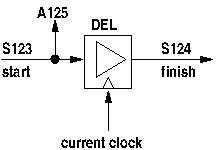
\includegraphics{assert1}
        
        This simplified logic applies if there is no enclosing {\bf priwait()} and hence {\bf pri\_in} and
        {\bf pri\_out} are null. In that case the method could be written as -
        
        \begin{lstlisting}[gobble=8, language=threepl, numbers=left, numberstyle=\tiny, xleftmargin=1cm]
            .
            .  check input and output argument counts
            .
            Ref     oref = outargs.getRef(0, "assert() -");
            if (oref.getMode() != Mode.VALUE)
                throw new ExEx("assert() output argument must be value mode", loc);
            if (oref.getPrimType() != Ptype.LOG)
                throw new ExEx("assert() output argument must be type log", loc);
            
            TDEVar      start = tdelist.signal("S", loc);
            TDEVar      finish = tdelist.signal("S", loc);
            WordSpec    ws = new WordSpec(1, Ptype.LOG);
            TDEVar      tdev = tdelist.signal("A", ws, loc);
            Val         rval = new Val(null, Mode.STATIC, tdev, loc);
            
            rval.addOVar(getCurrentClockVar());
            oref.checkMatch(rval, false, "assert() ", loc);
            oref.assignTo(rval, loc);

            tdelist.connect(tdev, start);

            tdelist.del(finish, start, getCurrentClock(), esig);
            startl.add(start);
            finishl.add(finish);
        \end{lstlisting}
        {\bf oref} is a reference to the output value mode variable.\\
        {\bf start} is a signal we create for the execution thread input.\\
        {\bf finish} is a signal we create which passes on the execution thread.\\
        {\bf ws} is a WordSpec for the assertion output which is type "log".\\
        {\bf tdev} is the assertion output TDEVar with a unique identifier "A.....".\\
        {\bf rval} is a {\bf Val} class wrapper for {\bf tdev}.\\
        
        The assert() call could be enclosed within
        a priwait() in which case instead of simply connecting {\bf tdev} to {\bf start} the following
        would be required -
        
        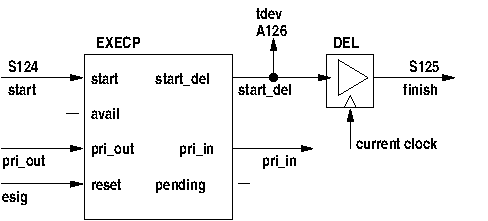
\includegraphics{assert2}
        
        To handle the priwait() an EXECP TDE is required. This can be generated by calling TDEList.execp().
        \begin{lstlisting}[gobble=8, language=java]
            if (pri_in == null)
                tdelist.connect(start_del, start);  // no waitpri
            else {
                TDEVar  v = tdelist.execp(null, start, pri_in, pri_out, esig, null, loc);
                tdelist.connect(start_del, v);
            }
        \end{lstlisting}
        
        
        If in addition we wish to implement the 2nd argument to assert() then an OR gate on the output
        is required -
        
        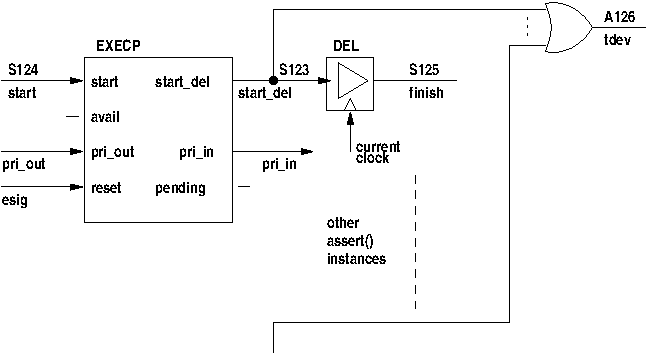
\includegraphics{assert3}

        \begin{lstlisting}[gobble=8, language=java]
            .
            .
            boolean or = false;
            if (inargs.size() == 1) {
                Val     or_val = inargs.getVal(0);
                if (or_val.getMode() != Mode.IMMEDIATE)
                    throw new ExEx("assert() input argument must be immediate mode", loc);
                if (or_val.getPrimType() != Ptype.LOG)
                    throw new ExEx("assert() input argument must be type log", loc);
                or = or_val.getSingleLval(loc);
            }
            .
            .
            if (or) {
                Var     ovar = oref.getVar();
                int     i = oref.getWordSpec().getWord(0);
                if (ovar.getVal(i) == null) {
                    // No initial value so just assign pulse signal.
                    oref.assignTo(rval, loc);
                } else {
                    // Assign OR of initial value and new pulse signal.
                    Val     oval = outargs.getVal(0);
                    TDEVar  otdev = oval.getTDEVar();
                    oref.assignTo(new Val(ovar, Mode.VALUE, tdelist.or(otdev, tdev, loc), loc), loc);
                }
            } else
                oref.assignTo(rval, loc);
            .
            .
        
        \end{lstlisting}
        Note that the previous value of the output argument value mode variable is ORed with the
        assert signal \lstinline[gobble=8, language=java]'tdelist.or(otdev, tdev, loc)'
        Where several assert() statements use the same output argument the assert signals
        will be chained together by ORs. These will later be optimised into a single wide gate
        (TDEList.java optimiseTDEList() line 1199).






\chapter{Netlist Code Generation}

    Netlist generation is done from the intermediate TDE list created during
    immediate execution.
    
    Thus far only Xilinx FPGAs have been catered for. The class structure
    is intended to allow convenient porting to other vendor FPGAs.

    The class structure is -

    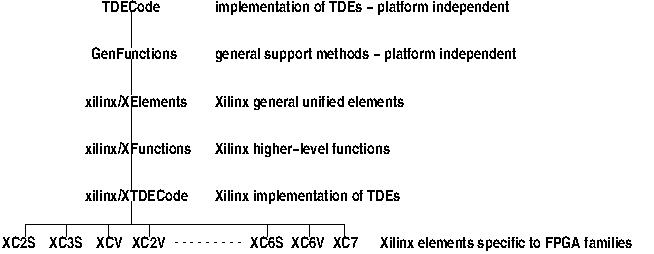
\includegraphics{netlist_classes}
    
    where each extends the class above. The FPGA object is one of the classes in
    the bottom row and it is assigned to public static variable -
    \begin{lstlisting}[gobble=4, language=java]
        public static TDECode family;
    \end{lstlisting}
    in source file {\bf ThreePL.java}.

    
    An attempt has been made to separate generic and platform-specific
    classes. The netlist code generation software is in directory
    {\bf netlist} and the only platform code so far is in directory
    {\bf netlist/xilinx}. The generic classes are -

    {\bf TDECode} - this is an abstract class which has three purposes -
    \begin{enumerate}
    \item   to provide a platform-independent template for netlist generation
            from the TDE list. Abstract methods in TDECode, one for each TDE,
            are overridden by methods in Xilinx/XTDECode.
    \item   to provide common methods for accessing dimensional parameters
            associated with each specific FPGA type. Examples are LUT input
            width, block RAM sizes and availability of 3-state drivers.
    \item   to optimise the netlist in a general sense - more netlist
            optimisation is done in xilinx/XTDECode where it is specific to
            the FPGA family.
    \end{enumerate}

    {\bf Element} - represents an FPGA hardware element.

    {\bf Net} - represents a net.

    {\bf GenFunctions} - contains methods to extract subarrays of nets, construct
    lists of arguments, change the width of net arrays, generate strings,
    generate net arrays representing constants and connect nets and net arrays.

    {\bf NetConstants} - an interface supplying some enums used in netlist
    optimisation.

    {\bf Ports} - a description of the input, output and 3-state output pins
    of a particular element type (not of an instance of the element). This is
    used when generating each cell description in the netlist file.

    {\bf Display}, {\bf NetListDraw}, {\bf Properties}, {\bf SigList} - these
    classes implement the schematic netlist display invoked by the -d option
    on the 3PL command line.
    
    \section{The Element class}
    
        
This class represents an element, for example a flip-flop,
a gate or a block of RAM.


{\bf String cellname} - the element name to be used in the netlist, e.g.
"FDRS" or "AND2".

{\bf String ident} - a unique identifier string of the form "b123" (see
{\bf icount} below).


{\bf private static HashMap\verb'<'String, Ports\verb'>' celldecls} -  a
map of cell types. The map key is the cell name and the value is class {\bf
Ports} describing the input and output ports. Ports contains 3 sets,
inputs, outputs and 3-state outputs. Each of these sets contains Strings
giving the port names.


{\bf HashSet\verb'<'String\verb'>' inportset} - this is a set of the input
pins for the element. It will be a common set for the element type stored
in an instance of the {\bf Ports} class kept in a static map {\bf
celldecls} (see below).

{\bf HashSet\verb'<'String\verb'>' outportset} - like inportset above this
is a set of output pins for the element.

{\bf HashSet\verb'<'String\verb'>' tsportset} -  like inportset above this
is a set of 3-state output pins for the element.

The above sets are the same sets as those contained in the Ports class in
the 'celldecls' map indexed by the cell name of this instance. When a port
connection is added to an element the port name is checked against the
appropriate set and if not present is added. Since the port sets are shared
among elements with the same cell name the port sets for an element type
are built up by usage and are not pre-defined. This can be a problem where
nested gates are combined into a single gate during optimisation since that
element prototype might not have been encountered during netlist building.
For that reason AND, OR, XOR, XNOR gates and LUTs are initialised in map
{\bf celldecls} for number of inputs from 1 to the LUT width
(XTDECode.initialise())

{\bf HashMap\verb'<'String, Net\verb'>' inports} - a map
of input ports where the map key is the port name and the value is an
instance of class Net.

{\bf HashMap\verb'<'String, Net\verb'>' outports} -  a
map of 2-state output ports where the map key is the port name and the
value is an instance of class Net.

{\bf HashMap\verb'<'String, Net\verb'>' tsports} -  a map
of 3-state output ports where the map key is the port name and the value
is an instance of class Net.

Maps 'inports', 'outports' and 'tsports' represent the input and output
connections to the element. The keys to these maps are the port name
strings and the associated values are the connected nets (class 'Net').


{\bf Gtype element\_type} - a gate type enum used to identify elements
that can be optimised. The gate type enums are defined in class {\bf
NetConstants}.

{\bf private static ArrayList\verb'<'Element\verb'>' instances = new
ArrayList\verb'<'Element\verb'>'(20000)} - a list of all elements in the
netlist. Optimisable elements are added to the front of the list and a
count of these is kept in static variable {\bf ocount}.
Elements whose type is NONE are added at the end of the list, all others
being inserted at the front. Thus the elements that are labeled as being
subject to optimisation are located at the head of list 'instances'. The
number of such entries in the list is given by 'ocount'. This scheme avoids
traversing the whole list of elements when performing an optimisation pass.

{\bf String expression} - if a logical expression was used to generate a
property, for example an expression for a LUT, then that expression is
stored here. It is kept in this field for display purposes but is
translated into a hexadecimal string and stored in field 'property\_init'
for later inclusion in the netlist file as an INIT property to initialise
the element (LUT contents or flip-flop initial state).

{\bf String property\_init} - properties of the element. This might be
initialisation for a LUT or a flip-flop.

{\bf public static Element gnd} \\
{\bf public static Element vcc} -
publicly available GND and VCC elements. These are assigned in the
constructor XElements() where also publicly available Nets {\bf LO} and
{\bf HI} are created and connected to their output ports.

{\bf int count = 0} - this is a counter used for the schematic netlist
display to identify elements shown more than once in the schematic in
which case they are coloured to highlight the fact.

{\bf private static int ocount = 0} - count of optimisable elements -
see above.

{\bf private static int icount = 0} - unique integer for generating cell
identifiers (see {\bf ident} above). It is incremented after each use.

NOTE: when 3PL is run repeatedly via the GUI, class TDECode and all
subclasses down to the class specific to the FPGA family are
constructed afresh. Thus all static variables are re-created. Classes
Element and Net are NOT reconstructed and hence static variables in
these classes must be explicitly re-initialised on each run! In the case
of this class this is done by method init().


The following subsections describe constructors and methods. Many
simple methods which only provide read or write access to class
variables are omitted.

\subsection{constructors}

    \begin{lstlisting}[gobble=4, language=java]
        public Element (String name) { makeElement(name, null, Gtype.NONE); }
    \end{lstlisting}

    Construct a general element. These are given the gate type
    Gtype.NONE and are not subject to nelist optimisation. Parameter
    {\bf name} is the element name, e.g. "IBUF". The resulting element
    is given an arbitrary unique netlist block name of the form "b123".

    \begin{lstlisting}[gobble=4, language=java]
        public Element (String name, String bname) { makeElement(name, bname, Gtype.NONE); }
    \end{lstlisting}

    Construct a general element. These are given the gate type
    Gtype.NONE and are not subject to nelist optimisation. The block
    name must be unique. Parameter {\bf name} is the element name, e.g.
    "IBUF". Parameter {\bf bname} is the netlist block name.

    \begin{lstlisting}[gobble=4, language=java]
        public Element (String name, Gtype element_type) { makeElement(name, null, element_type); }
    \end{lstlisting}

    Construct a gate element. The gate type is used to direct netlist
    optimisation. Parameter {\bf name} is the element name, e.g. "IBUF".
    Parameter {\bf element\_type} is the element gate type, e.g.
    Gtype.MUXCY The resulting element is given an arbitrary unique
    netlist block name of the form "b123".

    Each of these constructors calls the common private method
    {\bf makeElement()}. Each element is added to the static list
    {\bf instances}, optimisable elements at the front of the list
    to avoid traversing the whole list during optimisation.

\subsection{method init()}

    \begin{lstlisting}[gobble=4, language=java]
        public static void init () {
            icount = 0; // unique integer for identifiers
            ocount = 0; // count of optimisable elements
            celldecls = new HashMap<String, Ports>();
            instances = new ArrayList<Element>(20000);
        }
    \end{lstlisting}

    This method initialises static variables. This must be done
    by a method, rather than during class initialisation, to
    allow code generation to be restarted when 3PL is repeatedly run
    interactively from the GUI.

\subsection{method putCelldecl()}

    There are two signatures for this.

    \begin{lstlisting}[gobble=4, language=java]
        public static void putCelldecl (String name, int nports) {
            celldecls.put(name, gatePorts(nports));
        }
    \end{lstlisting}

    This method puts a logic gate cell declaration in the cell map.
    Normally the cell map is filled during calls to the constructors
    for class {\bf Element}, but gate elements are entered explicitly
    to ensure that gate of all possible widths are present. This is
    because optimisation might reduce say an AND3 gate to an AND2 gate
    but the latter may not have been encountered in calls to the
    constructor.

    \begin{lstlisting}[gobble=4, language=java]
        public static void putCelldecl (String name, ArrayList inports, ArrayList outports) {
            .
            .
            .
        }
    \end{lstlisting}

    This method puts a general cell declaration in the cell map. This
    is used for elements specific to particular FPGAs, e.g. MULT18X18
    or DSP48E and ensures that all inputs and outputs are included in
    the definition even if they are not included during a call to
    a constructor.

\subsection{method gatePorts()}

    \begin{lstlisting}[gobble=4, language=java]
        public static Ports gatePorts (int n) {
            Ports   p = new Ports();
            p.outports.add("O");
            for (int i=0 ; i<n ; i++)
                p.inports.add("I" + i);
            return(p);
        }
    \end{lstlisting}

    This method creates a port class for a gate element. The parameter
    indicates the number of input ports and there is one output port.

\subsection{adding inputs}

    To add a single Net to a named port -
    \begin{lstlisting}[gobble=4, language=java]
        public void addInput (String port, Net n) {
            switch (element_type) {
            case AND:
            case OR:
            case XOR:
                break;
            default:
                inportset.add(port);
            }
            if (n == null)
                return;
            inports.put(port, n);
            n.connect(this, port, PortType.INPORT);
        }
    \end{lstlisting}
    AND, OR and XOR gates have varying numbers of inputs and are subject
    to changes to the number of inputs during optimisation, so the input
    port set should not be touched. It can be assumed that the input
    port sets for all these gates that are within the accepted number of
    inputs for the FPGA family will have been already created. For all
    others the port string is added to the set of inports for this
    element type. The last statement creates a reciprocal link from the
    Net to this element.

    To add an array of Nets -
    \begin{lstlisting}[gobble=4, language=java]
        public void addInputArray (String port, Net[] n) {
            if (n == null)
                return;
            for (int i=0 ; i<n.length ; i++)
                addInput(port + i, n[i]);
        }
    \end{lstlisting}
    The port string has "0", "1" etc. appended.

    To add an array of Nets with most significant bit padding -
    \begin{lstlisting}[gobble=4, language=java]
        public void addInputArray (String port, Net[] n, int size, Net pad) {
            int portnum = 0;
            int asize = (n == null) ? 0 : n.length;
            for (int i=0 ; i<asize ; i++)
                addInput(port + portnum++, n[i]);
            for (int i=asize ; i<size ; i++)
                addInput(port + portnum++, pad);
        }
    \end{lstlisting}
    The port string has "0", "1" etc. appended. If the array is smaller
    than the designated size the remaining inputs are connected to
    Net {\bf pad}. If the array is null all inputs are connected to
    Net {\bf pad}.

    To add an array of Nets with least significant bit padding -
    \begin{lstlisting}[gobble=4, language=java]
        public void addInputArrayTop (String port, Net[] n, int size, int max, Net pad) {
            int npad = max - size;
            int asize = (n == null) ? 0 : n.length;
            int portnum = 0;
            for (int i=0 ; i<npad ; i++)
                addInput(port + portnum++, pad);
            for (int i=0 ; i<size ; i++)
                addInput(port + portnum++, (i < asize) ? n[i] : Net.LO);
        }
    \end{lstlisting}
    If the Net array is smaller than {\bf size} then the most
    significant bits are padded as well.

    To add an array of Nets across two different ports -
    \begin{lstlisting}[gobble=4, language=java]
        public void addInputArray (
            String  port1,
            String  port2,
            Net[]   n,
            int     size1
        ) {
            int portnum1 = 0;
            int portnum2 = 0;
            int asize = (n == null) ? 0 : n.length;
            for (int i=0 ; i<asize ; i++)
                if (i < size1)
                    addInput(port1 + portnum1++, n[i]);
                else
                    addInput(port2 + portnum2++, n[i]);
        }
    \end{lstlisting}
    Parameter {\bf port1} is the first input port identifying string
    head. Parameter {\bf port2} is the second input port identifying
    string head. Parameter {\bf n} is the net array. Parameter {\bf
    size1} is the number of ports using the first head string.

    To add an array of Nets across two different ports with most
    significant bit padding -
    \begin{lstlisting}[gobble=4, language=java]
        public void addInputArray (
            String  port1,
            String  port2,
            Net[]   n,
            int     size1,
            int     size,
            Net     pad
        ) {
            int portnum1 = 0;
            int portnum2 = 0;
            int asize = (n == null) ? 0 : n.length;
            for (int i=0 ; i<asize ; i++)
                if (i < size1)
                    addInput(port1 + portnum1++, n[i]);
                else
                    addInput(port2 + portnum2++, n[i]);
            for (int i=asize ; i<size ; i++)
                if (i < size1)
                    addInput(port1 + portnum1++, pad);
                else
                    addInput(port2 + portnum2++, pad);
        }
    \end{lstlisting}



\subsection{adding outputs}

    For output Net and Net arrays these follow the same pattern as
    for inputs above -
    \begin{lstlisting}[gobble=4, language=java]
        public void addOutput (String port, Net n) {
            outportset.add(port);
            if (n == null)
                return;
            if (n.getNumOutputs() != 0)
                throw new ExEx("net 2nd source");
            outports.put(port, n);
            n.connect(this, port, PortType.OUTPORT);
        }
    \end{lstlisting}
    There is a builtin check here to ensure that the Net is not
    connected to any other element outputs. The last statement creates a
    reciprocal link from the Net to this element.

    And similarly -
    \begin{lstlisting}[gobble=4, language=java]
        public void addOutputArray (String port, Net[] n)
        public void addOutputArray (String port1, String port2, int size1, Net[] n)
    \end{lstlisting}

    For 3-state outputs -
    \begin{lstlisting}[gobble=4, language=java]
        public void addTS (String port, Net n) {
            tsportset.add(port);
            if (n == null)
                return;
            tsports.put(port, n);
            n.connect(this, port, PortType.TSPORT);
        }
    \end{lstlisting}


\subsection{method removeNet}

    This method removes a Net connected to an Element. The argument
    is the port to which the Net is connected.
    \begin{lstlisting}[gobble=4, language=java]
        public void removeNet (String port) {
            if (inports.containsKey(port)) {
                inports.get(port).disconnect(this, port);
                inports.remove(port);
            } else if (outports.containsKey(port)) {
                outports.get(port).disconnect(this, port);
                outports.remove(port);
            } else if (tsports.containsKey(port)) {
                tsports.get(port).disconnect(this, port);
                tsports.remove(port);
            } else
                throw new ExEx("net not connected to element");
        }
    \end{lstlisting}
    The code checks the input, output and 3-state port maps in turn
    looking for the port name string as key. Inputs are searched first
    as they are the more numerous. The get() method returns the Net
    and the disconnect() method removes the Element from the Net.
    The remove() then removes the key and associated value ()Net from
    the particular Element port map.


\subsection{method remapInputs}

    This method re-names the input ports of a gate Element. It is
    required when one or more inputs have been removed as a result
    of optimisation.
    \begin{lstlisting}[gobble=4, language=java]
        public void remapInputs () {
            int         n = inports.size();
            HashMap     ports_new = new HashMap();
            Net         inet;
            int         i = 0;
            for (Map.Entry me : inports.entrySet()) {
                String      newport = "I" + i++;
                String      port = (String)me.getKey();
                inet = (Net)me.getValue();
                inet.changePort(this, port, newport);
                ports_new.put(newport, inet);
            }

            inports = ports_new;
            cellname = element_type.toString() + n;

            Ports p;
            if (celldecls.containsKey(cellname)) {
                p = celldecls.get(cellname);
                inportset = p.inports;
                outportset = p.outports;
                tsportset = p.tsports;
            } else {
                // Remapped wide gates may not have declared cell
                // set entries - dont worry as wide gates will
                // be converted so will never need these sets anyway.
                inportset = null;
                outportset = null;
                tsportset = null;
            }
        }
    \end{lstlisting}
    The input port map is traversed and the Nets are placed in a new map
    where the keys (port names) are allocated sequentially as "I0",
    "I1" etc. That new map is then assigned as a replacement input port
    map. The Element cell name is changed to reflect the ne winput count,
    e.g. "AND5" may now be "AND3". The new cell name is now checked
    in the cell declaration map and if present the port sets for the
    Element are assigned from that map. If not present it means that
    the gate is a wide gate which has not been entered in
    the cell declaration map since it will be converted to use available
    library elements later.

\subsection{method changeElement()}

    This method changes an element. This is used during optimisation to
    change an element into another. Previous connections are optionally
    stripped. Parameter {\bf name} is the new element name, e.g. "INV".
    Parameter {\bf element\_type} is the element gate type, e.g.
    Gtype.INV. Parameter {\bf strip} if true results in the element being
    stripped of input and output Nets. An example might be an XOR2 gate
    with one input connected to VCC being changed to an INV of the
    other input.

    \begin{lstlisting}[gobble=4, language=java]
        public void changeElement (String name, Gtype element_type, boolean strip) {
            Ports   p;
            if (strip)
                strip();
            cellname = name;
            this.element_type = element_type;
            if (celldecls.containsKey(name))
                p = celldecls.get(name);
            else {
                p = new Ports();
                celldecls.put(name, p);
            }
            if (strip) {
                inports = new HashMap<String, Net>();
                outports = new HashMap<String, Net>();
                tsports = new HashMap<String, Net>();
            }
            inportset = p.inports;
            outportset = p.outports;
            tsportset = p.tsports;
        }
    \end{lstlisting}
    The Element is first optionally stripped of all inputs and outputs,
    depending on boolean argument {\bf strip}. The cell name string
    and element type are then overwritten from the supplied arguments.
    If the new element is contained in the cell declaration map then
    the ports sets are obtained from that map, otherwise new sets are
    created for the named cell. If the element has been stripped of
    connections then new port maps are created, otherwise the existing
    port maps remain. The port sets are then assigned from the sets
    obtained from the cell declarations map.

\subsection{method strip()}

    This method disconnects the Element from all input and output
    nets and then clears all input and output port maps. This is used
    prior to deleting an Element or changing all its port
    connections during optimisation.
    \begin{lstlisting}[gobble=4, language=java]
        public void strip () {
            for (Map.Entry me : inports.entrySet()) {
                String      pinname  = (String)me.getKey();
                Net         net = (Net)me.getValue();
                net.disconnect(this, pinname);
            }
            inports.clear();
            for (Map.Entry me : outports.entrySet()) {
                String      pinname  = (String)me.getKey();
                Net         net = (Net)me.getValue();
                net.disconnect(this, pinname);
            }
            outports.clear();
            for (Map.Entry me : tsports.entrySet()) {
                String      pinname  = (String)me.getKey();
                Net         net = (Net)me.getValue();
                net.disconnect(this, pinname);
            }
            tsports.clear();
        }
    \end{lstlisting}

\subsection{method addExpression()}

    This method adds an expression to a LUT. The expression string
    is kept for display purposes and is also translated into a
    property value for LUT initialisation. Parameter {\bf s} is the
    expression string.
    \begin{lstlisting}[gobble=4, language=java]
        public void addExpression (String s) {
            expression = s;
            property_init = Functions.bit_pattern(s, TDECode.lutwidth);
        }
    \end{lstlisting}

\subsection{method addProperty()}

    This method adds a property for LUT initialisation. Parameter
    {\bf s} is the property string.
    \begin{lstlisting}[gobble=4, language=java]
        public void addProperty (String s) {
            if (s == null)
                return;
            if (property_init != null)
                throw new ExEx("element INIT property multiply defined");
            property_init = s;
        }
    \end{lstlisting}



\subsection{methods for writing to the netlist file}

    Method
    \begin{lstlisting}[gobble=4, language=java]
        static public void outputCells (PrintWriter pw, String view)
    \end{lstlisting}
    outputs the cell port definitions to the EDIF netlist.
    Only cells which have been instantiated are written out.
    Some cells may have been optimised out such that no instances
    remain in which case they are not written to the EDIF file cell
    definition section. Parameter {\bf pw} is the output interface to
    the EDIF netlist file and Parameter {\bf view} is the EDIF view
    parameter (the string "view\_1" seems to be required and this
    originates in codegen.TDEList.ncode()).

    Method
    \begin{lstlisting}[gobble=4, language=java]
        static public void outputInstances (PrintWriter pw, String view)
    \end{lstlisting}
    outputs all Elements to the EDIF netlist.

    Method
    \begin{lstlisting}[gobble=4, language=java]
        static public void outputConstraints (String group, PrintWriter pw)
    \end{lstlisting}
    outputs all element constraints for a group. Parameter {\bf pw} is
    the output interface to the constraint file for the group (name.ncf
    for group "n" and name.ucf for group "u"). Note that this method is
    called from netlist.xilinx.XTDECode() which also writes net
    constraints and general constraints to constraint files.

        

 
    \section{The Net class - a net label}
    
        The {\bf Net} class is small, its main function being to hold a net
identifier and associated NET class instance. The net connections to
elements are instances of class {\bf Net} (a net identifier wrapper),
not class {\bf NET} (the actual net). When two {\bf Net}s are connected
together it is not necessary to visit all elements to which the {\bf
Net}s are connected, instead one of the associated {\bf NET} class
instances is merged into the other and both {\bf Net} instances now
contain the same {\bf NET} instance.

A {\bf Net} constructor which is not passed an identifier will create
one consisting of "n" with an appended unique integer.

The member variables for {\bf Net} are -

{\bf private String id} - the net identifier.

{\bf private NET net} - the actual net.

There are six other member variables, input\_elements, input\_ports, output\_elements,
output\_ports, input\_index and output\_index, which are just temporary variables
used when traversing connected elements.

There are some class variables -

{\bf private static int icount} - an integer used to form unique
net identifiers of the form "n123". It is incremented after each use.

{\bf private static int hashcode\_count} - an integer used to form a
crude unique hash code for use by methods {\bf equals()} and {\bf
hashCode()} on instances of class {\bf NET}. These methods are used by
HashMap and HashSet classes to distinguish or equate NET class
instances.

{\bf private static HashMap\verb'<'String, Net\verb'>' identmap = new HashMap\verb'<'String,
Net\verb'>'(20000)} - a map of nets. The key is a net identifier and the
associated value is class Net.

{\bf private static HashSet\verb'<'NET\verb'>' instances = new HashSet\verb'<'NET\verb'>'(20000)} -
the set of NETs. This set is traversed when writing nets to the netlist
file.

{\bf public static Net LO} \\
{\bf public static Net HI} -
globally available GND and VCC nets. {\bf LO} and {\bf HI} are assigned
in the constructor XElements() because they are then connected there to
newly constructed Elements GND and VCC.




For an operation on a net the net identifier is used to extract the
{\bf Net} class instance from static map {\bf instances}. The {\bf Net}
in turn contains variable {\bf net}, class {\bf NET}, which is the
actual net. Many instances of net identifier class {\bf Net} will
contain the same actual {\bf NET}, meaning that they are connected.

The main methods are described in the following subsections.

\subsection{constructors and class creation methods}

    Constructor {\bf Net()} creates an un-named net with a unique
    identifier of the form "n123".

    A net with a constructed identifier can also be produced by
    constructor
    \begin{lstlisting}[gobble=4, language=java]
        public Net (String header)
    \end{lstlisting}
    which creates a net with a unique identifier by concatenating a
    unique integer to the header string supplied. This is used for
    signals which are not derived from source code variables but which
    are easier to trace in the netlist if given meaningfull identifier
    headers.

    A named Net can be constructed using constructor
    \begin{lstlisting}[gobble=4, language=java]
        public Net (String ident, boolean large)
    \end{lstlisting}
    which creates a net using the supplied identifier. The second
    parameter {\bf large}, if true, causes lists inside class
    NET to be created with a large initial size (10000) instead of the
    default size. This is used for Nets {\bf GND} and {\bf VCC} as they have
    a very large number of connections.

    A named net can also be constructed using method
    \begin{lstlisting}[gobble=4, language=java]
        static public Net get (String ident)
    \end{lstlisting}
    which returns a named net if it already exists and otherwise
    constructs it.

    An array of unnamed Nets can be created by method
    \begin{lstlisting}[gobble=4, language=java]
        static public Net[] netArray (int size)
    \end{lstlisting}
    where parameter {\bf size} provides the dimension of the array.

\subsection{method init()}

    This method re-initialises the class static variables prior
    to any run of 3PL.

\subsection{method equals()}

    \begin{lstlisting}[gobble=4, language=java]
        public boolean equals (Object o)
    \end{lstlisting}
    This method returns true if the argument is the same Net or
    is connected to the object Net (they share the same NET class
    instance). If the argument is null or not class Net then
    false is returned.

\subsection{connection to an Element}

    \begin{lstlisting}[gobble=4, language=java]
        public void connect (Element e, String port, PortType type)
    \end{lstlisting}
    This method connects a Net to an Element port but only modifies the
    Net structure, not that of the Element to which it connects. This is
    only called from methods {\bf addInput()}, {\bf addOutput()} or {\bf
    addTS()} in class Element which handle the related changes in that
    class.

\subsection{disconnection from an Element}

    \begin{lstlisting}[gobble=4, language=java]
        public void disconnect (Element e, String port)
    \end{lstlisting}
    This method disconnects a Net to an Element port but only modifies
    the Net structure, not that of the Element to which it is connected.
    The method is only called in -
    \blist
    \item   Element.strip()
    \item   Element.removeNet()
    \item   TDECode.optimiseXOR()
    \item   TDECode.inputEliminate()
    \blend
    In each case related changes to the Element are carried out
    elsewhere


\subsection{connection to another Net}

    \begin{lstlisting}[gobble=4, language=java]
        public void connect(Net n) {
            if (n.equals(LO) || n.equals(HI)) {
                n.connect(this);
                return;
            }

            if (this.equals(n))
                throw new ExEx("SYSTEM ERROR - netlist self-connect");

            if ((getNumOutputs() + n.getNumOutputs()) > 1) {
                msg("connection of nets will result in multiple sources");
                .
                .
                .

            }

            // Add all element connections of the new Net to this Net.
            net.nets.addAll(nnet.nets);
            net.elements.addAll(nnet.elements);
            net.ports.addAll(nnet.ports);
            net.porttypes.addAll(nnet.porttypes);
            net.inports += nnet.inports;
            net.outports += nnet.outports;
            net.tsoutports += nnet.tsoutports;

            // Add in the new ident list.
            net.idents.addAll(nnet.idents);

            // Append UCF and NCF strings from Net n to this Net.
            addConstraints("U", nnet.getConstraints("U"));
            addConstraints("N", nnet.getConstraints("N"));

            instances.remove(n.net);

            // Change all Nets associated with n.net to reference net.
            for (Net nn : nnet.nets)
                nn.net = net;
        }
    \end{lstlisting}
    This method connects two Nets. It does this by effectively
    merging the two NET subclasses so the the Nets share the same
    NET subclass; it adds the data from one NET to the other NET
    then deletes the former. It also traverses all Nets from the merged
    NET to change their nested NET class instance to the merged
    instance. If the argument Net is connected to GND or VCC then
    the method calls itself with the object and argument interchanged.
    This is to ensure that the Net identifier "GND" or "VCC"
    remains at the head of the list of connected identifiers and
    hence when {\bf setPrefIdent()} is called from TDEList.ncode()
    the "GND" or "VCC" will be encountered first in the list and will
    be set as the final preferred identifier (otherwise an "OPAD..."
    identifier might be encountered and prevail and the GND net in
    the netlist file would be labelled thus).             

\subsection{method addProperty()}

    \begin{lstlisting}[gobble=4, language=java]
        public void addProperty (String p, String v) {
            net.properties.put(p,  v);
        }
    \end{lstlisting}
    This method adds a property string to a net. P is the property identifier
    and v is the value string.

\subsection{Output Net instance to the EDIF netlist file}

    \begin{lstlisting}[gobble=4, language=java]
        static public void outputInstances (PrintWriter pw)
    \end{lstlisting}
    This method writes all Net instances to the EDIF file including
    all Element port connections.

    
    \section{The NET class - a net}
        
        The NET class represents a net. It will usually be linked from more than one
instance of class Net. Class Net represents a particular net identifier.
Class NET represents a net of multiple connected net identifiers.

Class NET has the following variables -

\blist
\item   {\bf ArrayList\verb'<'String\verb'>'} idents - a list of all identifiers associated
        with this net, i.e. which are in the linked Net class instances
\item   {\bf ArrayList\verb'<'Net\verb'>'} nets - a list of the linked Net class instances
\item   {\bf String} prefident - the prefered identifier, selected from the
        associated identifiers
\item   {\bf ArrayList\verb'<'Element\verb'>'} elements - an ordered list of Element class
        instances to which this net is connected
\item   {\bf ArrayList\verb'<'String\verb'>'} ports - an ordered list of port names corresponding
        to the elements above
\item   {\bf ArrayList\verb'<'PortType\verb'>'} porttypes - an ordered list of port types
        corresponding to the elements above (INPORT, OUTPORT, TSPORT)
\item   {\bf int} inports - the number of input ports to which this net is connected
\item   {\bf int} outports - the number of output ports to which this net is connected
\item   {\bf int} tsoutports - the number of 3-state output ports to which this net is connected
\item   {\bf public  TreeMap\verb'<'String,String\verb'>'} properties = new TreeMap\verb'<'String,String\verb'>'() -
        a map of XDC properties for this net; actually only PULLUP and PULLDOWN
\item   {\bf public  TDEVPtype} extport = TDEVPtype.NONE - the port type if
        an EDIF external port - one of NONE, INPUT, OUTPUT or INOUT
\item   {\bf public  String} extportname - the port name if an external EDIF port
\blend

Methods for this class are -

public void setPrefIdent () - traverse the list of equivalent identifiers for this net
and select the most "convenient" to appear in the EDIF netlist, copying it to
field prefident. GND and VCC are obvious, and any starting with PORT or glob. are
also desirable.

public String getEDIFIdent () - return the prefered identifier modified for
EDIF syntax, removing a leading underscors and replacing '[' and ']' with an
underscore.

public Net getNet () - get the first class Net from the list of linked Net class
instances.

public boolean isExtOutPort () - return true if this is an EDIF output or 3-state
output port.

        

    \section{The structure of the internal netlist}
    
        The Element class represents logic elements and the Net class the
        signals connecting element pins. The following figure illustrates this -

        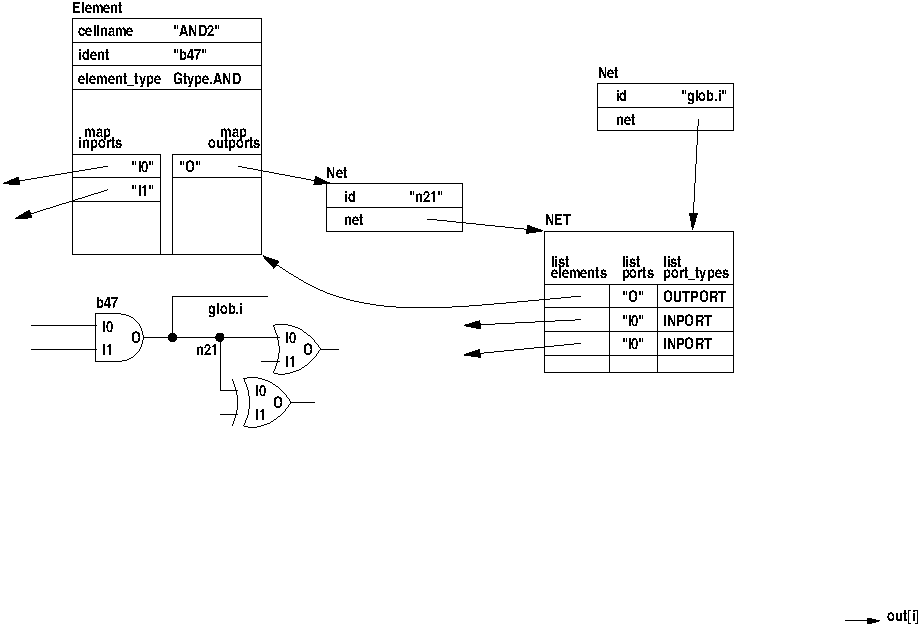
\includegraphics{elements_nets}
        
        In this example nets "glob.i" and "n21" represent the same net, thus
        each is represented by a Net class instance but both contain the same
        NET subclass repreenting the actual net.

    \section{The TDECode class}
    
        The TDECode class has the following class variables -

{\bf static TDEVPtype[] ptypes = {TDEVPtype.INPUT, TDEVPtype.OUTPUT, TDEVPtype.INOUT}} -
an array to convert a numeric port type of 0, 1 or 2 from a TDEPORT TDE
into a TDEVPtype enum used for entries in {\bf ext\_port\_dirs}
(described below).

{\bf static ArrayList\verb'<'Object\verb'>' ext\_ports} - a list of external
ports, each member is a Net or else a port identifier string.

{\bf static ArrayList\verb'<'TDEVPtype\verb'>' ext\_port\_dirs} - a list of
port types, i.e. input, output or 3-state output.

{\bf static ArrayList\verb'<'String\verb'>' ext\_port\_pins} - a list of port
pins where these are FPGA pads.

{\bf static TreeMap\verb'<'String,Object\verb'>' portmap} is a map of ports where
the key is either the port identifier of else the port Net.

The following member variables contain information about the target FPGA.

\blist
\item   {\bf String} fname - name of the FPGA family

\item   {\bf int} lutwidth - number of inputs to CLB LUT

\item   {\bf int} dspregwidth - effective width of multiplier/DSP
                                         block when used as a register

\item   {\bf int} srladdrwidth - shift register address width

\item   {\bf int} addsubinputwidth - maximum adder/subtracter input width

\item   {\bf int} multinputwidth - maximum multiplier input width

\item   {\bf int} divinputwidth - maximum divider input width

\item   {\bf int} ramb\_ports - maximum number of block RAM ports

\item   {\bf boolean[]} ramb\_readable - which block RAM ports are readable

\item   {\bf boolean[]} ramb\_writable - which block RAM ports are writable

\item   {\bf int[]} ramb\_dwidths = new int[20] - block RAM data widths for address widths

\item   {\bf int} ramb\_addrmin[] - block RAM smallest address width for \verb'#' of ports

\item   {\bf int} ramb\_addrmax[] - block RAM largest address width for \verb'#' of ports

\item   {\bf int} ramc\_ports - maximum number of CLB RAM ports

\item   {\bf boolean[]} ramc\_readable - which CLB RAM ports are readable

\item   {\bf boolean[]} ramc\_writable - which CLB RAM ports are writable

\item   {\bf int[]} ramc\_dwidths = new int[20] - CLB RAM data widths for address widths

\item   {\bf int} ramc\_addrmin[] - CLB RAM and ROM smallest address width for \verb'#' of ports

\item   {\bf int} ramc\_addrmax[] - CLB RAM port max block address width for \verb'#' of ports

\item   {\bf int} romc\_addrmin[] - CLB ROM port min block address width for \verb'#' of ports

\item   {\bf int} romc\_addrmax[] - CLB ROM port max block address width for \verb'#' of ports

\item   {\bf int[]} queue\_buffer\_cram\_depths - allowed depths for CLB RAM queue buffers

\item   {\bf int} queue\_buffer\_min\_cram\_depth - smallest depth for CLB RAM queue buffers

\item   {\bf int} queue\_buffer\_max\_cram\_depth - largest depth for CLB RAM queue buffers

\item   {\bf int[]} queue\_buffer\_rram\_depths - allowed depths for block RAM queue buffers

\item   {\bf int} queue\_buffer\_min\_rram\_depth - smallest depth for block RAM queue buffers

\item   {\bf int} queue\_buffer\_max\_rram\_depth - largest depth for block RAM queue buffers

\item   {\bf boolean} defaultOutputDirect - is the output mode direct flag default?

\item   {\bf boolean} defaultStaticContinuous - is the static mode continuous flag default?

\item   {\bf boolean} deviceHasTBUF - does device have 3-state buffers?

\item   {\bf boolean} deviceAllowsQueue - does device allow queue mode?
                                         queues require memory

\item   {\bf boolean} deviceAllowsCMemory - does device allow cmemory mode?
                                         requires CLB RAM

\item   {\bf boolean} deviceAllowsRMemory - does device allow rmemory mode?
                                         requires block RAM

\item   {\bf int} ramc\_mux\_addr\_bits\_maxc - CLB RAM address bits beyond maximum
                                         the number of extra address bits for
                                         CLB RAM gained by MUXing

\item   {\bf boolean} deviceFDRSEpatch - change FDRSE to FDCE + logic for CPLD

\item   {\bf boolean} deviceCascadeGates - skip conversion of cascaded or wide gates

\item   {\bf boolean} deviceCPLDarith - use CPLD addition/subtraction logic
                                         i.e. simple logic instead of carry chain
\blend

These variables are assigned in the constructor for the FPGA class, XC5V etc
which extend class TDECode.



The following methods return FPGA parameters derived from the above class
variables -
\blist
\item   LUTWidth() - return the LUT width for the FPGA
\item   AddSubWidth() - return the maximum adder/subtracter input
        width for the FPGA (9999 for no explicit limit)
\item   DivWidth() - return the maximum divider input width
        for the FPGA (9999 for no explicit limit)
\item   SRLAddrWidth() - return the maximum SRL (shift register)
        input width for the FPGA (0 if there is no SRL element)
\item   cramPorts() - return the number of memory ports for
        combinatorial-output RAM
\item   rramPorts() - return the number of memory ports for
        registered-output RAM
\item   cramAwidthMax() - return the maximum address width for a
        combinatorial-output RAM
\item   rramAwidthMax() - return the maximum address width for a
        registered-output RAM
\item   rramDwidth() - return the data width associated with an address
        width for a registered-output RAM
\item   cramReadable() - determine if a combinatorial-output RAM port is
        readable
\item   cramWritable() - determine if a combinatorial-output RAM port is
        writable
\item   rramReadable() - determine if a registered-output RAM port is
        readable
\item   rramWritable() - determine if a registered-output RAM port is
        writable
\item   queueDepthUsingCram() - determine if a requested queue buffer
        depth using combinatorial output memory is allowed
\item   queueDepthUsingRram() - determine if a requested queue buffer
        depth using registered output memory is allowed
\item   minQueueDepth() - return the minimum asynchronous queue depth
\item   maxQueueDepth() - return the maximum queue depth
\item   outputDirect() - determine if the output mode 'direct' attribute
        should be default for this device
\item   defaultContinuous() - determine if the selectvalue mode
        'continuous' attribute should be default for this device
\item   hasTBUF() - determine if this device has internal 3-state
        buffers
\item   allowQueue() - determine if queue mode variables are allowed for
        this device
\item   allowCMemory() - determine if cmemory mode variables are allowed
        forthis device
\item   allowRMemory() - determine if rmemory mode variables are allowed
        forthis device
\item   needFDRSEpatch() - determine if this device requires gates to
        fully implement an FDRSE flip-flop
\item   needCascadeGates() - determine if this device must construct
        wide AND or OR gates by cascading, rather than using inbuit
        MUXes or a carry chain
\item   needCPLDarith() - determine if special arithmetic for CPLDs is
        needed; this means that addition and subtraction and magnitude
        comparisons will be done by gate logic rather than using carry
        chains
\blend

Abstract method outputExterns() writes all external ports to the EDIF netlist
file. This method is overridden in class XTDECODE for Xilinx.

The following methods optimise the netlist code and are described
elsewhere.
\blist
\item   optimiseGNDandVCC()
\item   optimiseINV()
\item   optimiseAND()
\item   optimiseOR()
\item   optimiseXOR()
\item   unNest()
\item   inputEliminate()
\item   optimiseLUT()
\item   optimiseFDRS()
\item   remapInputs()
\blend









The remainder of the methods are abstract and are overridden by
methods in xilinx.XTDECode. All except the last seven are methods
to convert TDEs to internal netlist constructs. The method names
are self explanatory -
\blist
\item   TDESELECT()
\item   TDETSELECT()
\item   TDEREG()
\item   TDEINV()
\item   TDEAND()
\item   TDEOR()
\item   TDEXOR()
\item   TDEDFF()
\item   TDEIBUF()
\item   TDEOBUF()
\item   TDESTART()
\item   TDEILOOP()
\item   TDEWHEN()
\item   TDEWHILE()
\item   TDEDOWHILE()
\item   TDERESYNC()
\item   TDESAMPLE()
\item   TDEEXECP()
\item   TDECONNECT()
\item   TDEOPERATOR()
\item   TDEWAIT()
\item   TDEDEL()
\item   TDEDIVERGE()
\item   TDEQUEUEBUFFER()
\item   TDEPRIORITY()
\item   TDECRAM()
\item   TDERRAM()
\item   TDECLOCK()
\item   TDECLOCKINFO()
\item   TDEELEMENT()
\item   TDEELEMENTCONNECT()
\item   TDEPORT()
\item   TDESPECIAL()
\blend

The last seven abstract methods are miscellaneous. Again they are
overridden by methods in xilinx.XTDECode.

TDEOptimise() applies family-specific optimisations to the TDE list.

optimise() carries out low-level optimisation of the internal netlist
structure.

convert() converts generic gate elements to appropriate elements
for the target device. Before this is called the netlist structure
might contain an AND gate with 10 inputs. Following conversion that
element would have been replaced perhaps by 3 4-input LUTs connected
to carry chain MUXCYs.

verify() examines all elements to ensure there are no errors or
inconsistencies. This method is not located in class netlist.Element
as the checks are specific to target device elements rather than
generic elements (there is however a method netlist.Net.verify()
to check nets and this is generic since nets are not specific to
the target device).

netFromPin() returns the identifier of the net attached to a pad
given the pad identifier.

EDIFFileNameExtension() returns the EDIF file extension.


Abstract method outputConstraints() writes constraints to the approprite file(s)
(for Xilinx this is the ISE NCF or Vivado XDC file). This method is overridden in
class XTDECODE for Xilinx.

        
        
    \section{The GenFunctions class}
    
        GenFunctions extends TDECode. The methods in this class provide
such general functions as -

\blist
\item   conversion between arrays and ArrayLists of Nets
\item   padding or sign extension of arrays of Nets
\item   extraction of sub-arrays of Nets
\item   padding or truncation of strings
\item   generation of hexadcimal strings from integers
\item   extraction of a bit from a hexadecimal string
\item   conversion of constants to arrays of Net
\item   connections between Nets and Net arrays
\blend

The methods are sufficiently simple that they are not listed or
described here.

        
    

    \section{The xilinx/XC... FPGA family classes}
    
        Each of these classes extends XTDECode. One of these classes is
        instantiated as the object representing the FPGA or CPLD.
        These classes are specific to Xilinx FPGA families and are
        named appropriately -
        
        \blist
        \item   UNISIMS - Xilinx common library elements
        \item   XC2C - Xilinx Coolrunner II CPLD
        \item   XC2S - Xilinx Spartan 2C FPGA
        \item   XC3S - Xilinx Spartan 3S FPGA
        \item   XCV - Xilinx Virtex FPGA
        \item   XC2V - Xilinx Virtex 2 FPGA
        \item   XC2VP - Xilinx Virtex 2 PRO FPGA
        \item   XC4V - Xilinx Virtex 4 FPGA
        \item   XC5V - Xilinx Virtex 5 FPGA
        \item   XC6S - Xilinx Spartan 6 FPGA
        \item   XC6V - Xilinx Virtex 6 FPGA
        \item   XC7 - Xilinx 7-series
        \item   XC95 - Xilinx XC9500 CPLD
        \blend
        
        The UNISIMS class represents Xilinx common library elements but
        really these are already implemented in the super classes
        XFunctions and XElements so UNISIMS is really just a default
        object when no specific target device is specified.
        
        XC2C and XC95 are CPLDs, not FPGAs. Much of the functionality of
        3PL can be used with these devices but there are limitations.
        
        These device-specific classes perform two functions -
        
        \blist
        \item   they provide parameters and flags to superclasses to
                tailor logic generation for the specific device, e.g.
                LUT inputs, CLB RAM sizes, block RAM sizes
        \item   they provide methods for elements specific to the
                device, e.g. block RAM, DSP blocks
        \blend

        

    \section{The xilinx/XElements class}
    
        XElements extends GenFunctions to vendor-specific elements. The methods generate
basic elements such as gates and flip-flops.

The IBUF Element provides a simple example -
\begin{lstlisting}[gobble=0, language=java]
    public Element IBUF (Net o, Net i) {
        Element c = new Element("IBUF");
        c.addInput("I", i);
        c.addOutput("O", o);
        return(c);
    }
\end{lstlisting}
The new Element is created by a constructor, the element name
string being passed as an argument to the constructor. The input
and output Nets are added paired with the port name strings. The
Element is returned.

Where an Element may be subject to later optimisation a gate type
is added, e.g. the XORCY Element -
\begin{lstlisting}[gobble=0, language=java]
    public Net XORCY (Net li, Net ci) {
        Element c = new Element("XORCY", Gtype.XORCY);
        Net     o = new Net();
        c.addInput("LI", li);
        c.addInput("CI", ci);
        c.addOutput("O", o);
        return(o);
    }
\end{lstlisting}
In this case the output Net is returned.

The following basic Elements are constructed directly -

\blist
\item   LUT - a 1 to n input look-up table
\item   INV - inverter
\item   AND - 1 to n input AND gate
\item   OR - 1 to n input OR gate
\item   XOR - 1 to n input XOR gate
\item   XNOR - 1 to n input XNOR gate
\item   SRL16E - 16 bit CLB shift register
\item   SRL32E - 32 bit CLB shift register
\item   FDRS - reset/set flip-flop
\item   FDCP - clear/preset flip-flop
\item   MULT\_AND - multiplier AND
\item   MUXCY - carry multiplexer
\item   MUXF5 - CLB multiplexer
\item   MUXF6 - CLB multiplexer
\item   XORCY - carry XOR
\item   BUFG - global clock buffer
\item   IPAD - input pad
\item   OPAD - output pad
\item   IOPAD - bi-directional pad
\item   BUFE - internal 3-state buffer, +ve enable
\item   BUFT - internal 3-state buffer, -ve enable
\item   IBUF - input buffer
\item   IBUFDS - differential input buffer
\item   IBUFG - input global clock buffer
\item   IBUFGDS - differential input global clock buffer
\item   OBUF - output buffer
\item   OBUFDS - differential output buffer
\item   PULLDOWN - internal longline pulldown
\item   PULLUP - internal longline pullup
\item   RAM\_1 - single port CLB RAM
\item   ROM\_1 - single port CLB ROM
\item   RAM\_2 - dual port CLB RAM
\blend

Other Elements available in some Xilinx FPGA families but not others
have methods which must be overridden in subclasses -

\blist
\item   MULT18X18 - 18 x 18 bit multiplier
\item   MULT18X18S - 18 x 18 bit multiplier with output register
\item   MULT25X18 - 25 x 18 bit multiplier
\item   MULT25X18S - 25 x 18 bit multiplier with output register
\item   MULREG - multiplier used as register only
\item   ramallocate - block RAM
\item   fifoallocate - block RAM as FIFO
\item   FIFO - FIFO using dual port block RAM
\item   Mult- multiplier
\item   dsp48\_alu - an ALU using a DSP block
\blend
These are overridden in subclasses XC2V, XC2VP etc. where appropriate.

This subdivision is somewhat arbitrary; some Elements in the first
group are not available in some FPGAs or CPLDs and conditional code
ensures that these are not called is such cases. For consistency some
of these should be moved to the second group and the methods moved
into subclasses.


    
    
    \section{The xilinx/XFunctions class}
    
        XFunctions extends XElements.

This class is the heart of the code (netlist) generation. It has methods
which use the Elements created in class XElements to provide higher
level functions such as registers, multiplexers and queue buffers.

The following functional elements are implemented by methods
in this class -

\blist
\item   registers - to implement static mode variables and to provide
        registers for other methods in this class
\item   resynchroniser - to transfer a pulse from one clock domain to
        another
\item   queue buffers - to implement queue mode variables
\item   delay line - to implement the TDEDEL intermediate code element
\item   shifters - to implement left and right constant and variable
        shift
\item   adder - to implement addition
\item   inverter - to implement bit inversion
\item   incrementer - to implement addition by 1
\item   subtracter - to implement subtraction
\item   decrementer - to implement subtraction by 1
\item   adder/subtracter - to implement selectable addition or
        subtraction
\item   ALU - to implement addition/subtraction/assignment in CLBs
\item   incrementer/decrementer - to implement selectable addition or
        subtraction of 1
\item   signed and unsigned multipliers - to implement multiplication
        using hardware if available and CLB logic otherwise
\item   signed and unsigned divider/remainder - to implement to
        implement division and remaindering using CLB logic
\item   numerical comparators - to implement equal, not equal,
        greater than, greater than or equal, less than and less than or
        equal numerical comparisons
\item   combinatorial RAM and ROM - to implement cmemory mode variables
\item   registered output RAM - to implement rmemory mode variables
\blend

\subsection{registers}

    \begin{lstlisting}[gobble=4, language=java]
        public Net[] reg (
            Net[]               in,
            Net                 c,
            Net                 ce,
            Net                 r,
            String              sinit,
            ArrayList<String>   constraints
        ) {
            int                 width = in.length;
            Net[]               out = new Net[width];
            ArrayList<String>   locs = new ArrayList<String>();

            // Constraints here are single strings -
            //  "TNM=..."
            //  "LOC=..."
            //  "DSP"
            // having been modified in XTDECode.TDEREG() from the key=value pairs
            // in the original TDE list.
            // Location constraints should be one per bit.
            // The DSP constraint is ignored.
            if (constraints != null) {
                Iterator<String>    it = constraints.iterator();
                while (it.hasNext()) {
                    String s = it.next();
                    if (s.startsWith("LOC=")) {
                        locs.add(s);
                        it.remove();
                    }
                }
            }
            if (sinit == null)
                sinit = "0";
            for (int bit=0 ; bit<width ; bit++) {
                if (!locs.isEmpty())
                    constraints.add(0, locs.get(0));
                if ((strhexbit(sinit, bit) & 1) == 0)
                    out[bit] = FDRS(in[bit], c, ce, r, null, "R", constraints);
                else
                    out[bit] = FDRS(in[bit], c, ce, null, r, "S", constraints);
                if (!locs.isEmpty()) {
                    locs.remove(0);
                    constraints.remove(0);
                }
            }
            return(out);
        }
    \end{lstlisting}
    This method creates a register which has a single clock enable and
    single reset common to all flip-flops in the register. It is called
    from XTDECode.TDEREG() to create a static mode variable that is one
    bit wide and from several methods in this class to create registers.
    It is only in the former case that the constraints argument will be
    non-null.

    The code first searches the constraints list for location
    constraints (they start with "LOC="). It removes these, copying them
    to a new list. As each bit is created a location constraint is
    copied from the list (if there are any) and is put back at the
    front of the constraints list. At the end of the loop that location
    constraint is removed from both lists.

    If there is no initialisation string the string "0" is assigned.

    For each register bit the appropriate bit is extracted from the
    initialisation string using method strhexbit() from class
    genFunctions. Method FDRS() from class XElements is then called
    with either an "R" or "S" property argument and the reset signal
    is connected to either the R or S input as appropriate.

    \begin{lstlisting}[gobble=4, language=java]
        public Net[] reg (
            Net[]       in,
            Net         c,
            Net[]       ce,
            Net[]       r,
            String      sinit,
            ArrayList   constraints
        ) {
            int         width = in.length;
            Net[]       out = netArray(width);
            ArrayList   locs = new ArrayList();
            boolean     dsp = false;

            .
            . code for use of multiplier/DSP register
            .

            if (sinit == null)
                sinit = "0";
            out = new Net[width];
            for (int bit=0 ; bit<width ; bit++) {
                if (!locs.isEmpty())
                    constraints.add(0, (String)locs.get(0));
                if ((strhexbit(sinit, bit) & 1) == 0)
                    out[bit] = FDRS(in[bit], c, ce[bit], r[bit], null, "R", constraints);
                else
                    out[bit] = FDRS(in[bit], c, ce[bit], null, r[bit], "S", constraints);
                if (!locs.isEmpty()) {
                    locs.remove(0);
                    constraints.remove(0);
                }
            }
            return(out);
        }
    \end{lstlisting}
    This method differs from the previous in two respects -
    \blist
    \item   if there is no DSP constraint it is very similar to the
            previous method except that the clock enable and reset signals
            are now arrays, one for each flip-flop, rather than common
            single signals
    \item   if there is a DSP constraint, the register is not
            initialised and the FPGA has a hardware multiplier or DSP block
            then the register is implemented using the output register
            of a multiplier or DSP block
    \blend

    A map, {\bf hm}, and two classes, {\bf Cer} and {\bf Group}, were
    defined in the method for use when a DSP constraint is acted upon.
    These are used to group flip-flops within the register which share
    the same clock enable and reset signals. Each such group is
    implemented in a separate multiplier or DSP block since the clock
    enables and resets are common to all bits in those hardware
    registers. If a group entry is larger than the width of the hardware
    register then multiple units will be used. The {\bf Cer} class contains a
    Net pair, a clock enable and a reset. These are used as the key to
    map {\bf hm} which thus has an entry for each unique pair. The
    associated map value is class {\bf Group} which has an input list and an
    output list. These contain the input and output signals of
    flip-flops in each CE/R group in LSB to MSB bit order.

    The declarations are -
    \begin{lstlisting}[gobble=4, language=java]
        HashMap     hm = null;
        class Cer {
            Net ce;
            Net r;

            Cer (Net ce, Net r) {
                this.ce = ce;
                this.r = r;
            }

            public boolean equals (Object o) {
                return(ce.equals(((Cer)o).ce) && r.equals(((Cer)o).r));
            }
            public int hashCode () {
                return((ce.hashCode() << 16) + r.hashCode());
            }
        }
        class Group {
            ArrayList   inputs = new ArrayList();
            ArrayList   outputs = new ArrayList();
        }
    \end{lstlisting}
    The equals() and hashCode() methods are implemented to enable
    correct functioning of HashMap keys.

    The code to create the group data structure is -
    \begin{lstlisting}[gobble=4, language=java]
        hm = new HashMap();
        for (int i=0 ; i<width ; i++) {
            Cer x = new Cer(ce[i], r[i]);
            if (!hm.containsKey(x))
                hm.put(x, new Group());
            Group g = (Group)hm.get(x);
            g.inputs.add(in[i]);
            g.outputs.add(out[i]);
        }
    \end{lstlisting}

    The code to create the register is -
    \begin{lstlisting}[gobble=4, language=java]
        Iterator    mit = hm.entrySet().iterator();
        while (mit.hasNext()) {
            Map.Entry   me = (Map.Entry)mit.next();
            Cer         cer = (Cer)me.getKey();
            Group       g = (Group)me.getValue();
            Net[]       gout = new Net[1];
            Net[]       gin = new Net[1];
            int         gwidth = gout.length;
            int         mwidth = DSPRegWidth();
            int         k;
            int         l = gwidth;
            gout = (Net[])g.outputs.toArray(gout);
            gin = (Net[])g.inputs.toArray(gin);

            for (int j=0 ; j<gwidth ; j+=mwidth, l-=mwidth) {
                k = (l >= mwidth) ? j + mwidth - 1 : j + l - 1;
                MULREG(subarray(gin, j, k), subarray(gout, j, k), c, cer.ce, cer.r);
            }
        }
        return(out);
    \end{lstlisting}
    This iterates through the entries in the map converting each group
    into a register using one or more multipliers or DSP blocks. The
    cell type of Element(s) produced is MULREG which is later converted
    to MULT18X18 or DSP48E depending on the FPGA type (method {\bf
    convertElements()} in classes {\bf XC2VP}, {\bf XC5V} etc.).


\subsection{resynchroniser}

    A resynchroniser generates a pulse in another clock domain from a
    rising edge. When the input rises the rise is captured by the next
    input clock edge and an output pulse of one period duration is
    generated on the next output clock edge. This method is used
    by intermediate code TDE {\bf TDERESYNC} and also indirectly by
    methods {\bf async\_buffer()} and {\bf triggerbuffer(}) (via
    {\bf asynch\_fifo\_control()}) in this class.

    The logic circuit used is -

    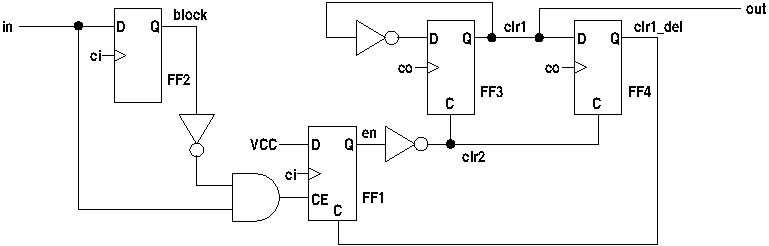
\includegraphics{resync}

    Note that FF1, FF3 and FF4 have asynchronous clear inputs. Initially
    all flip-flop outputs are low, thus {\bf block} and {\bf clr1}/{\bf
    out} are low. When {\bf in} goes high both FF1 and FF2 outputs go
    high on the next edge of clock {\bf ci}, the input clock. The {\bf
    CE} input of FF1 goes low as {\bf block} is now high. Since {\bf en}
    is now high, {\bf clr2} is low and this enables FF3 to toggle on the
    next edge of {\bf co}, the output clock, raising the output {\bf
    out}. On the next edge of {\bf co} FF3 toggles low again and FF4 is
    set, raising {\bf clr1\_del}, which clears FF1. When {\bf en} thus
    goes low {\bf clr2} goes high clamping FF3 low and clearing FF4. FF1
    is now free to again latch an input however if {\bf in} is still
    high {\bf block} will disable FF1. Thus {\bf in} must be clocked low
    to lower {\bf block} before FF1 can again start the pulse cycle.
    This circuit avoids race conditions between flip-flops in the two
    clock domains.

    The code to generate this is -

    \begin{lstlisting}[gobble=4, language=java]
        public Net resync (Net in, Net ci, Net co) {
            Net en;
            Net block;
            Net clr1 = new Net();
            Net clr1_del = new Net();
            Net clr2;

            block = FDRS(in, ci, null, null, null, null, null);
            en = FDCP(Net.HI, ci, AND(in, INV(block)), clr1_del, null, null, null);
            clr2 = INV(en);
            clr1.connect(FDCP(INV(clr1), co, null, clr2, null, null, null));
            clr1_del.connect(FDCP(clr1, co, null, clr2, null, null, null));
            return(clr1);
        }
    \end{lstlisting}
    Note the use of the connect() method. For example in the statement
    \begin{lstlisting}[gobble=4, language=java]
        clr1.connect(FDCP(INV(clr1), co, null, clr2, null, null, null));
    \end{lstlisting}
    the output Net is also used as an input argument, i.e. there is
    feedback. Thus the Net {\bf clr1} is declared and assigned a new
    instance, then passed as an input argument. The result returned from
    the call is then connected to Net {\bf clr1}. It cannot be assigned
    as that would overwrite the previous Net instance. A similar though
    more indirect argument applies to Net {\bf clr1\_del}.



\subsection{queue buffers}

    These were described in some detail in the section on intermediate
    code TDEs. Some of that description is repeated here.

    There are five methods for generating queue buffers -
    \blist
    \item   queuebuffer() - synchronous 2-deep default queue buffer
    \item   sync\_buffer() - synchronous n-deep queue buffer
    \item   async\_buffer() - asynchronous n-deep queue buffer
    \item   triggerbuffer() - synchronous or asynchronous n-deep queue
            buffer with no data
    \item   queueunbuffered() - a synchronous 0-deep queue buffer (no buffer)
    \blend

    \subsubsection{queuebuffer()}

        This method creates a synchronous queue buffer of depth 2.
        The logic for the default synchronous queue buffer of depth
        two is -

        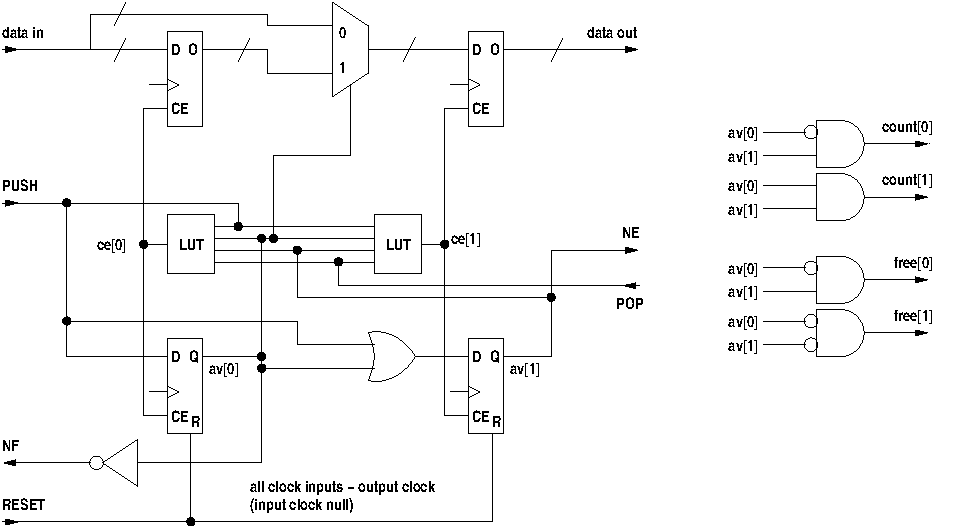
\includegraphics{queuebuffer}

        The 2-input multiplexer shown uses a 3-input LUT per bit.

        When PUSH is high input data is latched into one of two
        registers. If the buffer is empty the data is latched into the
        rightmost register to which the data output is directly
        connected. If another datum is written to the queue buffer it
        goes into the second (left) register. When a datum is popped the
        two registers are shifted right. This scheme avoids having
        combinatorial logic at the output thus minimising
        clock-to-data-out time. The tradeoff is a longer input setup
        time. The two flip-flops represent the occupancy status of the
        two registers. Each register/flip-flop pair has a common clock
        enable controlled by a 4-input LUT.

        The truth table for the control logic is as follows -

        \sf{\small{
        \begin{tabular}{ | c | c | c | c | | c | c | c | | c | c | c | c | c | c | l }
        \cline{1-13}
        \multicolumn{7}{| c ||}{t} & \multicolumn{6}{ c |}{t+1} & \\
        \cline{1-13}
          &    & \multicolumn{2}{ c ||}{av} & \multicolumn{2}{ c |}{ce} & & \multicolumn{2}{ c |}{av}
          & \multicolumn{2}{ c |}{ce} & & & \\
        PUSH & POP & [0] & [1] & [0] & [1] & MUX & [0] & [1] & [0] & [1] & NE & NF & \\
        \cline{1-13}
        \cline{1-13}
        0 & 0 & 0 & 0 & 0 & 0 & X & 0 & 0 & 0 & 0 & 0 & 1 & empty \\
          &   & 0 & 1 & 0 & 0 & X & 0 & 1 & 0 & 1 & 1 & 1 & 1 entry \\
          &   & 1 & 0 & - & - & - & - & - & - & - & - & - & illegal state \\
          &   & 1 & 1 & 0 & 0 & X & 1 & 1 & 1 & 1 & 1 & 0 & full \\
        \cline{1-13}
        0 & 1 & 0 & 0 & - & - & - & - & - & - & - & - & - & illegal state \\
          &   & 0 & 1 & X & 1 & X & 0 & 0 & 0 & 0 & 0 & 1 & av[1] $\downarrow$ POP, now empty\\
          &   & 1 & 0 & - & - & - & - & - & - & - & - & - & illegal state \\
          &   & 1 & 1 & 1 & 1 & 1 & 0 & 1 & 0 & 1 & 1 & 1 & av[0] $\downarrow$ POP, 1 remaining\\
        \cline{1-13}
        1 & 0 & 0 & 0 & 0 & 1 & 0 & 0 & 1 & 0 & 1 & 1 & 1 & av[1] $\uparrow$ PUSH, 1 entry\\
          &   & 0 & 1 & 1 & 0 & X & 1 & 1 & 1 & 1 & 1 & 0 & av[0] $\uparrow$ PUSH, now full\\
          &   & 1 & 0 & - & - & - & - & - & - & - & - & - & illegal state \\
          &   & 1 & 1 & - & - & - & - & - & - & - & - & - & illegal state \\
        \cline{1-13}
        1 & 1 & 0 & 0 & - & - & - & - & - & - & - & - & - & illegal state \\
          &   & 0 & 1 & 0 & 1 & 0 & 0 & 1 & 0 & 1 & 1 & 1 & 1 entry \\
          &   & 1 & 0 & - & - & - & - & - & - & - & - & - & illegal state \\
          &   & 1 & 1 & - & - & - & - & - & - & - & - & - & illegal state \\
        \cline{1-13}
        \end{tabular}
        }}

        {\bf PUSH} must not be raised when
        {\bf NF} is low and {\bf POP} must not be raised when
        {\bf NE} is low.

        The illegal states are described in the following table

        \sf{\small{
        \begin{tabular}{ c | c | c | c | c || l | }
        \multicolumn{6}{ c }{illegal states} \\
        & PUSH & POP & av[0] & av[1]  \\
        \hline
        1 & 0 & 0 & 1 & 0 & single entry must be at righXTDECode extends XFunctions. Its main function is to implement the
abstract methods in class TDECode which generate netlist code from
TDEs. These methods call methods in class xilinx/XFunctions which in
turn call methods in class xilinx/XElements.
t  \\
        2 & 0 & 1 & 0 & 0 & cannot pop when empty  \\
        3 & 0 & 1 & 1 & 0 & single entry must be at right  \\
        4 & 1 & 0 & 1 & 0 & single entry must be at right  \\
        5 & 1 & 0 & 1 & 1 & cannot push when full  \\
        6 & 1 & 1 & 0 & 0 & cannot pop when empty  \\
        7 & 1 & 1 & 1 & 0 & single entry must be at right  \\
        8 & 1 & 1 & 1 & 1 & cannot push when full  \\
        \hline
        \end{tabular}
        }}

        In entries 1, 3, 4 and 7 a single datum in the buffer must
        reside in the right register, so these states are not
        allowed.

        In entry 2 the registers are both empty and so a {\bf POP}
        is not allowed since there is no valid output ({\bf NE} is
        low). The logic has been designed so that no state change
        occurs, i.e. the {\bf POP} is ignored.

        In entry 6 the registers are both empty and so a {\bf POP}
        is not allowed since there is no valid output ({\bf NE} is
        low), however {\bf PUSH} is high. The logic has been designed
        so that the {\bf PUSH} is handled but the {\bf POP} is
        ignored.

        In entries 5 and 8 both registers are full and hence no {\bf
        PUSH} is allowed. Note that this is true even when {\bf POP}
        is asserted since we cannot allow {\bf NF} (not full) to
        depend on {\bf POP} or we generate the very logic cascade
        this buffering scheme was designed to avoid. The logic has
        been designed to ignore {\bf PUSH} in these cases.

        The truth tables for the two LUTs are -

        \sf{\small{
        \begin{tabular}{ l || c | c | c | c |}
        & PUSH & POP & av[0] & av[1]  \\
        \hline
        ce[0] & 0 & 1 & 1 & 1 \\
              & 1 & 0 & 0 & 1 \\
        \hline
        ce[1] & 0 & 1 & X & 1 \\
              & 1 & X & 0 & 0 \\
              & 1 & 1 & 0 & 1 \\
        \hline
        \end{tabular}
        }}

        The code for this is -

        \begin{lstlisting}[gobble=8, language=java]
            public Net[] queuebuffer (
                Net[]   in,     // data input
                Net     push,   // push-to-queue input
                Net     pop,    // pop-from-queue input
                Net     c,      // clock
                Net     ne,     // returned not empty signal
                Net     nf,     // returned not full signal
                Net     r,      // reset input
                Net     rr,     // reset output for chaining resets
                Net[]   count,  // returned buffer data count or null
                Net[]   free,   // returned free space count or null
                String  sinit   // initialisation hex string or null
            ) {
                int     width = in.length;
                String  id = (sinit != null) ? sinit : "";
                String  io =  (sinit != null) ? "S" : "R";

                Net[][] data = new Net[2][width];
                for (int i=0 ; i<2 ; i++)
                    for (int j=0 ; j<width ; j++)
                        data[i][j] = new Net();
                Net[]   av = new Net[2];
                Net[]   ce = new Net[2];

                av[0] = new Net("av0");
                av[1] = new Net("av1");
                ce[0] = LUT("(!I0*I1*I2*I3)+(I0*!I1*!I2*I3)", push, pop , av[0] , av[1]);
                ce[1] = LUT("(!I0*I1*I3)+(I0*!I2*!I3)+(I0*I1*!I2*I3)",
                                                        push, pop , av[0] , av[1]);
                if (in != null)
                    data[0] = reg(in, c, ce[0], null, null, null);
                av[0].connect(FDRS(push, c, ce[0], r, null, null, null));
                if (in != null)
                    data[1] = reg(mux2(av[0], in, data[0]), c, ce[1], r, id, null);
                av[1].connect(FDRS(OR(push, av[0]), c, ce[1], r, null, io, null));

                ne.connect(av[1]);
                nf.connect(INV(av[0]));

                if (count != null) {
                    count[0].connect(AND(av[1], INV(av[0])));
                    count[1].connect(AND(av[1], av[0]));
                }
                if (free != null) {
                    if (count != null)
                        free[0] = count[0];
                    else
                        free[0].connect(AND(av[1], INV(av[0])));
                    free[1].connect(AND(INV(av[1]), INV(av[0])));
                }

                if (rr != null) {
                    if (r != null)
                        rr.connect(r);
                    else
                        rr.connect(Net.LO);
                }

                if (in != null)
                    return(data[1]);
                else
                    return(null);
            }
        \end{lstlisting}
        Signals {\bf push} and {\bf pop} are control inputs with obvious
        functions. Signals {\bf ne} and {\bf nf} are argument Nets which
        are connected in the method to the logic signalling "not empty"
        and "not full". These are used to determine write and read
        availability respectively. Net {\bf r} is an optional reset
        input. Net {\bf rr} is a supplied Net which if not null
        is connected to the {\bf r} input if present, otherwise to GND.
        This output signal is available so that resets can be chained
        down a pipeline of queue variables.


    \subsubsection{sync\_buffer()}

        This method creates a synchronous queue buffer of depth greater
        than 2.
        A synchronous queue buffer of depth greater than two is
        implemented using either CLB dual port RAM or dual port
        block RAM. The CLB RAM is used for a depth of 16 and block
        RAM for greater depths.

        Because CLB RAM has combinatorial output and block RAM
        has registered output the CLB RAM is employed with a
        register appended to the output port so that the two
        forms of RAM can be used interchangably with the same
        control logic.

        The queue buffer is a queue. A required characteristic of
        queue buffers is that on writing a datum to an empty queue
        buffer that datum must be available on the next clock cycle.
        This presents a problem with a dual-port FIFO using
        registered output RAM because a read must be issued once the
        queue becomes non-empty, taking an extra cycle. This can be
        avoided by writing the first datum into a separate register
        rather than into the empty RAM. For CLB RAM this is easily
        implemented however in the case of block RAM the control
        logic for this is somewhat complicated. An easier solution
        for block RAM is to write the first datum into an empty
        queue via the read port rather than the write port. Since
        the queue is empty the read port is guaranteed to be unused
        on that clock cycle. Since the normal write mode for block
        RAM is WRITE\_FIRST and the CLB RAM with appended output
        register has been designed to behave the same way, the newly
        written datum will appear immediately in the output register
        upon writing. This avoids the extra cycle.

        For a block RAM the memory logic is -

        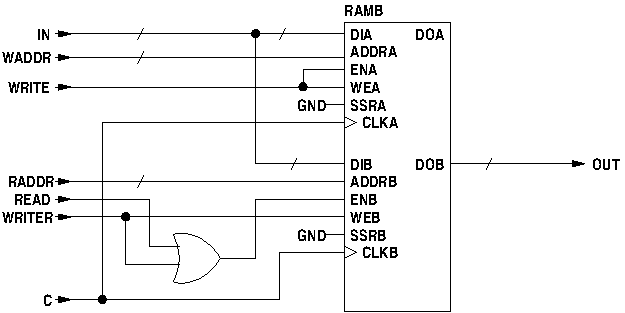
\includegraphics{qbram}

        To make an equivalent functional unit using CLB RAM
        the logic is -

        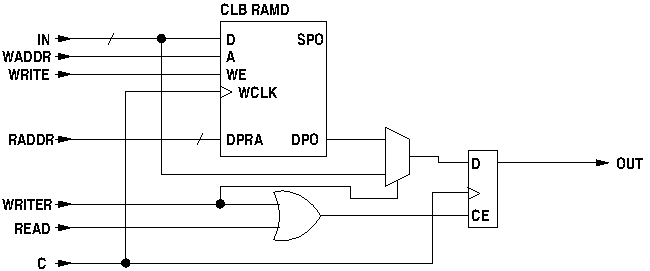
\includegraphics{qcram}

        In both the above blocks {\bf WRITER} writes directly to the
        output register whereas {\bf WRITE} writes to the RAM. {\bf
        READ} reads from the RAM to the output register.

        The code for the memory logic is contained in method
        queuemem() -
        \begin{lstlisting}[gobble=8, language=java]
            private Net[] queuemem (
                int     depth,  // buffer depth
                int     dwidth, // data width
                int     awidth, // address width
                Net[]   in,     // data input
                Net[]   raddr,  // read address
                Net[]   waddr,  // write address
                Net     read,   // read enable
                Net     write,  // write enable
                Net     writer, // write enable for the read port or null
                Net     ci,     // write clock
                Net     co      // read clock
            ) {
                Net[]   out;
                boolean is_sync = (ci == co);

                if (depth <= queue_buffer_max_cram_depth) {
                    // use CLB RAM
                    Net[] o = new Net[dwidth];
                    for (int i=0 ; i<dwidth ; i++)
                        o[i] = new Net("o" + i + "_");
                    sram2(  dwidth,
                              ci, write, waddr,   in, null,
                            null,  null, raddr, null,    o,
                            null, null );
                    if (is_sync)
                        out = reg(mux2(writer, o, in), co, read, null, null, null);
                    else
                        out = reg(o, co, read, null, null, null);
                    return(out);
                }

                // use block RAM
                out = new Net[dwidth];
                for (int i=0 ; i<dwidth ; i++)
                    out[i] = new Net("out" + i + "_");
                Net[]   rin = is_sync ? in : null;
                rram2 ( dwidth, awidth,
                        write,  write, ci, waddr,  in, null,
                         read, writer, co, raddr, rin,  out,
                        null, new ArrayList() );
                return(out);
            }
        \end{lstlisting}

        If the buffer depth is less than or equal to the maximum CLB RAM
        depth (TDECode.queue\_buffer\_max\_cram\_depth) then CLB RAM is
        used (method XFunctions.sram2()), otherwise block RAM is used
        (method XFunctions.rram2()). In the case of a synchronous buffer
        the first write to an empty FIFO asserts {\bf writer} which 
        casues the output register to be directly loaded with the datum.


        The following terms are used in the logic description -

        \blist
        \item   empty - the RAM is empty
        \item   full - the RAM is full
        \item   NE - data is available at the output of the queue buffer
        \item   NF - data can be written to the queue buffer
        \item   read - read RAM
        \item   write - write RAM
        \item   writer - first write when queue buffer empty
        \item   raddr - RAM read address
        \item   waddr - RAM write address
        \item   fcnt - RAM occupancy counter
        \item   $\Uparrow$ - increment
        \item   $\Downarrow$ - decrement
        \blend

        Note that a RAM occupancy counter, {\bf fcnt}, is kept in
        addition to read and write address counters. {\bf fcnt} is
        used to determine the RAM full and empty conditions and is
        potentially faster than doing comparisons between {\bf
        raddr} and {\bf waddr}. Additional counters are used for the
        optional word count and space count, again trading speed for
        logic and routing resources.

        The following table shows the change of state and counter
        increment/decrement operations in controlling the queue
        buffer ({\bf full} and {\bf NF} are not shown) -

        \sf{\small{
        \begin{tabular}{ | c | c | c | c || c | c | c | c | c | c | c |}
        \hline
        \multicolumn{2}{| c |}{state} &
        \multicolumn{2}{ c ||}{inputs} &
        \multicolumn{3}{ c |}{increment/decrement} &
        \multicolumn{3}{ c |}{memory control} &
        new \\
        \cline{1-10}
        empty & NE & PUSH & POP & waddr & raddr & fcnt & write & writer & read & NE\\
        \hline
        1 & 0 & 1 & 0 &            &            &              & 0 & 1 & 0 & 1 \\                     
        0 & 1 & 1 & 0 & $\Uparrow$ &            & $\Uparrow$   & 1 & 0 & 0 & 1 \\           
        1 & 1 & 1 & 0 & $\Uparrow$ &            & $\Uparrow$   & 1 & 0 & 0 & 1 \\           
        0 & 1 & 1 & 1 & $\Uparrow$ & $\Uparrow$ &              & 1 & 0 & 1 & 1 \\           
        1 & 1 & 1 & 1 &            &            &              & 0 & 1 & 0 & 1 \\                     
        0 & 1 & 0 & 1 &            & $\Uparrow$ & $\Downarrow$ & 0 & 0 & 1 & 1 \\       
        1 & 1 & 0 & 1 &            &            &              & 0 & 0 & 0 & 0 \\                    
        \hline
        \end{tabular}
        }}

        On first write to an empty queue buffer the datum is
        written directly to the read port of the RAM block and
        {\bf NE} goes high, but {\bf fcnt} stays at 0 as nothing is
        written to the RAM. The next write (if there is no read) will
        write to RAM and increment both{\bf fcnt} and {\bf waddr}. On
        acknowledging the output datum (i.e. popping a datum off
        the queue) if there is only the datum in the read port register
        {\bf NE} will go low since {\bf fcnt} is 0 ({\bf empty}
        will be true). If there is a datum in the output register and
        another in the RAM then the last RAM read to the port register
        will occur and {\bf fcnt} will decrement from 1 to 0 and
        empty will become true, but NE will not go low until the next
        {\bf POP}.

        Related equations -

        % NF = !full
        % read = POP & !empty
        % write = PUSH & NE & !(empty & POP)
        % writer = PUSH & empty & !(NE & !POP)                  
        $
        \mathsf{NF = \overline{full}} \\
        \mathsf{read = POP \cdot \overline{empty}} \\
        \mathsf{write = PUSH \cdot NE \cdot \overline{(empty \cdot POP)}} \\
        \mathsf{writer = PUSH \cdot empty \cdot \overline{(NE \cdot \overline{POP})}}
        $

        State changes -

        % NE <- !(empty & NE & !PUSH & POP)
        % empty <- !write & (fcnt==0 | fcnt==1 && read)
        % full <- !read & (fcnt==11...11 | fcnt==11...10 & write)
        $
        \mathsf{NE \Leftarrow \overline{empty \cdot NE \cdot \overline{PUSH} \cdot POP}} \\
        \mathsf{empty \Leftarrow \overline{write} \cdot (fcnt==0 + fcnt==1 \cdot read)} \\
        \mathsf{full \Leftarrow \overline{read} \cdot (fcnt==11\cdots11 + fcnt==11\cdots10 \cdot write)}
        $

        Increment/decrement counters -

        % raddr++ = read
        % waddr++ = write
        % fcnt++ = write & !read
        % fcnt-- = read & !write
        $
        \mathsf{raddr\Uparrow = read} \\
        \mathsf{waddr\Uparrow = write} \\
        \mathsf{fcnt\Uparrow = write \cdot \overline{read}} \\
        \mathsf{fcnt\Downarrow = read \cdot \overline{write}}
        $

        The code is -
        \begin{lstlisting}[gobble=8, language=java]
            public Net[] sync_buffer (
                Net[]   in,     // data input
                Net     push,   // write-to-queue input
                Net     pop,    // pop-from-queue input
                Net     c,      // clock
                Net     ne,     // returned not empty
                Net     nf,     // returned not full
                Net[]   count,  // returned buffer data count or null
                Net[]   free,   // returned free space count or null
                Net     r,      // buffer reset
                Net     rr,     // buffer reset output
                boolean fifo,   // use FIFO hardware if present
                int     depth,  // buffer depth - a power of 2 constrained by FPGA family
                Var     wcvar,  // write clock variable
                Var     rcvar   // read clock variable
            ) {
                int     dwidth = in.length;
                Net     empty = new Net("EMPTY");
                Net     full = new Net("FULL");

                if (((this instanceof XC5V) || (this instanceof XC6V)) && (depth >= 512) && (depth <= 8192) && fifo) {
                    // For Virtex5 or Virtex6 block RAM FIFO can use inbuilt FIFO logic.
                    if (rr != null) {
                        if (r != null)
                            rr.connect(r);
                        else
                            rr.connect(Net.LO);
                    }
                    ne.connect(INV(empty));
                    nf.connect(INV(full));
                    Net[]   out = new Net[dwidth];
                    for (int i=0 ; i<dwidth ; i++)
                        out[i] = new Net("out" + i + "_");
                    queuefifo(depth, in, push, pop, out, empty, full, count, free, r, c, c, wcvar, rcvar);
                    return(out);
                }

                int     awidth = bits(depth-1, false);
                Net     read = new Net("READ");
                Net     write = new Net("WRITE");
                Net     writer;
                Net[]   raddr, waddr, out;

                read.connect(AND(pop, INV(empty)));
                write.connect(AND(push, ne, INV(AND(empty, pop))));
                writer = AND(push, empty, INV(AND(ne, INV(pop))));
                ne.connect(FDRS(INV(AND(empty, ne, INV(push), pop)), c, OR(push, pop), r, null, null, null));
                nf.connect(INV(full));

                raddr = cb(awidth, false, c,  read, r, null, null);
                waddr = cb(awidth, false, c, write, r, null, null);

                int     cwidth = awidth + 1;
                Net[]   fcnt;
                Net     ed;
                Net     fd;

                fcnt = cb(awidth, false, c, XOR(read, write), r, read, null);

                ed = AND(INV(write), eqzeros(fcnt, 1, awidth-1), OR(INV(fcnt[0]), read));
                empty.connect(FDRS(ed, c, null, null, r, "S", null));
                fd = AND(INV(read), eqones(fcnt, 1, awidth-1), OR(fcnt[0], write));
                full.connect(FDRS(fd, c, null, r, null, null, null));

                if (count != null) {
                    Net[]   fcntr;
                    fcntr = cb(cwidth, false, c, XOR(pop, push), r, pop, null);
                    connect(count, fcntr);
                }
                if (free != null) {
                    Net[]   ecntr;
                    String  sinit = Integer.toHexString(1 << awidth);
                    ecntr = cb(cwidth, false, c, XOR(pop, push), r, push, sinit);
                    connect(free, ecntr);
                }

                Net mread = OR(read, writer);
                out = queuemem(depth, dwidth, awidth, in, raddr, waddr, mread, write, writer, c, c);
                if (rr != null) {
                    if (r != null)
                        rr.connect(r);
                    else
                        rr.connect(Net.LO);
                }
                return(out);
            }
        \end{lstlisting}
        Calls to constructor Net(), e.g. Net("EMPTY"), create nets which
        have unique identifiers constructed by appending an integer to
        the argument string. The head strings are chosen to label nets
        with meaningful identifiers in the netlist but have no other
        significance.

        If the FPGA is Virtex5 or Virtex6 and the buffer depth is
        between 512 and 8192 inclusive then method queuefifo() is called
        to use the inbuilt block RAM FIFO logic. This can be used for
        both synchronous and asynchronous buffers. The code for this
        method is -
        \begin{lstlisting}[gobble=8, language=java]
            private void queuefifo(
                int     depth,  // buffer depth
                Net[]   in,     // data input
                Net     push,   // true to push a datum
                Net     pop,    // true to pop a datum
                Net[]   out,    // data output
                Net     empty,  // true if the FIFO is empty
                Net     full,   // true if the FIFO is full
                Net[]   count,  // number of contained data
                Net[]   free,   // number of free spaces
                Net     r,      // reset signal or null
                Net     cw,     // write clock
                Net     cr,     // read clock
                Var     wcvar,  // write clock variable
                Var     rcvar   // read clock variable
            ) {
                int     dwidth = in.length;
                int     awidth = bits(depth-1, false);
                Net[]   rdcount = null;
                Net[]   wrcount = null;
                Net         r3 = new Net();
                double      minfreq = Math.min(wcvar.getClkMinFreq(), rcvar.getClkMinFreq());
                double      wcmaxfreq = wcvar.getClkFreq();
                int         rcycles = (int)(Math.ceil(wcmaxfreq / minfreq)) * 4;
                Net[]       srl16in = new Net[1];
                Net[]       srl16out = null;
                ArrayList   srl16init = new ArrayList();
                srl16in[0] = r3;

                for (int i=0 ; i<rcycles ; i++)
                    srl16init.add("1");
                srl16init.add("0");

                if (r != null)
                    srl16out = del(rcycles+1, srl16in, null, cw, OR(r, r3), null, srl16init);
                else
                    srl16out = del(rcycles+1, srl16in, null, cw, r, null, srl16init);
                srl16out[0].connect(r3);

                if (awidth < 9) // should have a variable for this
                    awidth = 9; // minimum block RAM address width (depth 512)

                int bdwidth = ramb_dwidths[awidth];
                int nb = (dwidth - 1) / bdwidth + 1;
                int totwidth = nb * bdwidth;

                if ((count != null) || (free != null)) {
                    rdcount = netArray(awidth);
                    wrcount = netArray(awidth);
                }

                for (int i=0 ; i<nb ; i++) {
                    int l = i * bdwidth;
                    int u = l + bdwidth - 1;
                    if (u >= dwidth)
                        u = dwidth - 1;
                    Net[]   id = (in != null) ? subarray(in, l, u) : null;
                    Net[]   od = (out != null) ? subarray(out, l, u) : null;

                    if (i == 0)
                        FIFO(   depth, id, push, pop, od, empty, full, rdcount, wrcount,
                                r3, cw, cr  );
                    else
                        FIFO(   depth, id, push, pop, od, null, null, null, null,
                                r3, cw, cr  );
                }

                // count and free only used for synchronous queues
                if (count != null) {
                    Net[] xx = sub(wrcount, rdcount, null, false, false);
                    for (int i=0 ; i<(count.length-1) ; i++)
                        count[i].connect(xx[i]);
                    count[count.length-1].connect(full);
                }
                if (free != null) {
                    Net[] yy = sub(rdcount, wrcount, null, false, false);
                    for (int i=0 ; i<(free.length-1) ; i++)
                        free[i].connect(yy[i]);
                    free[free.length-1].connect(full);
                }
            }
        \end{lstlisting}

        Net {\bf r3} is the FIFO reset. This must be high for at least 3
        clock cycles of both the read and the write clock. A reset must
        be done after power-up so is done after configuration. {\bf
        rcycles} is the number of cycles of the write clock {\bf cw}
        necessary for at least 3 cycles of both clocks. The reset pulse
        is generated using one or more CLB shift registers. The initial
        condition is 01...1, so the output is initially 1. The output is
        connected to the CE and the data input so the contents will
        shift until the 0 is at the output at which point it will stop.
        The external reset {\bf r} is ORed in to the CE to start the
        shift sequence of {\bf rcycles} 1s and a 0 each time.

    \subsubsection{async\_buffer()}

        For an asynchronous queue buffer the input and output clocks
        differ and the scheme for avoiding an initial read on a
        write to an empty queue buffer cannot be used. The point at
        which a queue becomes available after a write to an empty
        buffer is now undefined since the clocks are separate and
        unrelated.

        The CLB RAM block now simply has a register on the output
        of the read-only port.

        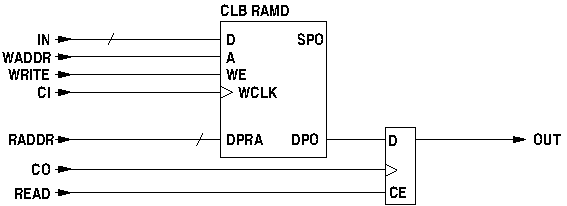
\includegraphics{aqcram}

        The block RAM has no additional logic.

        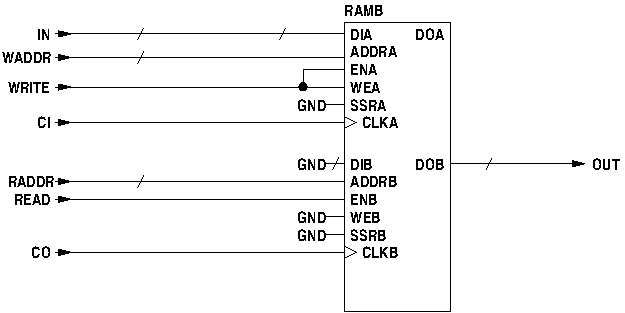
\includegraphics{aqbram}

        In method {\bf queuemem()} described previously the boolean {\bf
        is\_sync} selects whether this extra logic is inserted or not.

        The asynchronous queue buffer uses one of the above RAMs (the
        former for depth 16, the latter for greater depths) and an
        address generator block. The use of address comparison for
        full and empty determination means that the depth of the RAM
        FIFO is $2^n - 1$ however an additional datum is held in the
        RAM output register giving a total buffer depth of $2^n$.
        The additional logic shown provides the first read following
        a write to an empty buffer after which {\bf NE} is raised.

        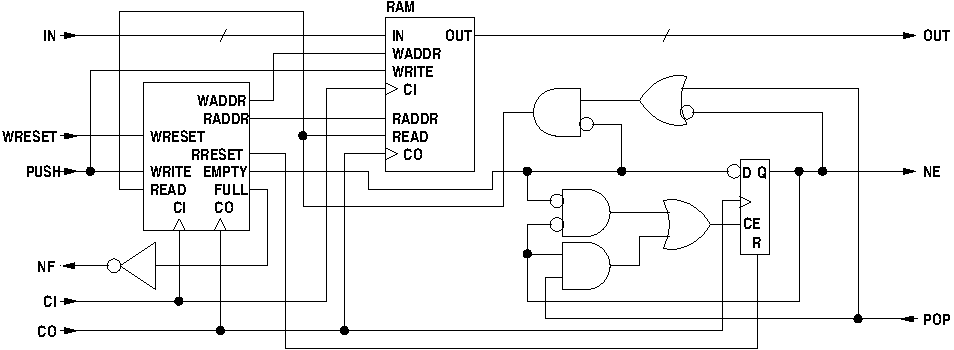
\includegraphics{asyncqueuebuffer}

        The code for this is -
        \begin{lstlisting}[gobble=8, language=java]
            public Net[] async_buffer (
                Net[]   in,     // the data input
                Net     push,   // push-to-queue input
                Net     pop,    // pop-from-queue input
                Net     ci,     // input clock
                Net     co,     // output clock
                Net     ne,     // returned not empty
                Net     nf,     // returned not full
                Net[]   wstat,  // returned status synchronised to the read clock
                Net[]   rstat,  // returned status synchronised to the write clock
                Net     r,      // reset input synchronised to the write clock or null
                Net     rr,     // reset output synchronised to the read clock or null
                boolean fifo,   // use FIFO hardware if present
                int     depth,  // buffer depth
                Var     wcvar,  // write clock variable
                Var     rcvar   // read clock variable
            ) {
                Net     full = new Net("FULL");
                Net     empty = new Net("EMPTY");
                int     dwidth = in.length;

                if (((this instanceof XC5V) || (this instanceof XC6V)) && (depth >= 512) && (depth <= 8192) &&
                    (wstat == null) && (rstat == null) && fifo) {
                    // For Virtex5 or Virtex6 block RAM FIFO can use inbuilt FIFO logic.
                    if (rr != null) {
                        if (r != null)
                            rr.connect(r);
                        else
                            rr.connect(Net.LO);
                    }
                    ne.connect(INV(empty));
                    nf.connect(INV(full));
                    Net[]   out = new Net[dwidth];
                    for (int i=0 ; i<dwidth ; i++)
                        out[i] = new Net("out" + i + "_");
                    queuefifo(depth, in, push, pop, out, empty, full, null, null, r, ci, co, wcvar, rcvar);
                    return(out);
                }

                int     awidth = bits(depth-1, false);
                Net[]   waddr = new Net[awidth];
                Net[]   raddr = new Net[awidth];
                Net     read;
                Net     write = push;
                Net[]   out;
                Net     oack;

                if ((rr == null) && (r != null))
                    rr = new Net("rr");

                nf.connect(INV(full));

                for (int i=0 ; i<awidth ; i++) {
                    waddr[i] = new Net("WADDR" + i + "_");
                    raddr[i] = new Net("RADDR" + i + "_");
                }

                oack = OR(AND(ne, pop), AND(INV(ne), INV(empty)));

                asynch_fifo_control (
                    write, ne, pop, ci, co, r,                      // input nets
                    waddr, raddr, rstat, wstat, full, empty, rr,    // output nets
                    awidth, depth
                );

                ne.connect(FDRS(INV(empty), co, oack, rr, null, null, null));

                read = AND(OR(INV(ne), pop), INV(empty));
                out = queuemem(depth, dwidth, awidth, in, raddr, waddr, read, write, null, ci, co);
                return(out);
            }
        \end{lstlisting}

        If the FPGA is Virtex5 or Virtex6 and the buffer depth is
        between 512 and 8192 inclusive and the write status ({\bf
        wstat}) and read status arguments ({\bf rstat}) are null and
        parameter {\bf fifo} is true then method {\bf queuefifo()} is
        called to use the FIFO logic associated with block RAMs (the
        read and write status cannot be derived from that logic).

        As in the schematic diagram above the two main blocks are
        memory (method {\bf queuemem()}) and asynchronous control
        logic (method {\bf asynch\_fifo\_control()}).


        Resetting an asynchronous queue buffer must be carried out with
        care. A pending read must be allowed to complete after which
        {\bf NE} will go low and no more reads will occur (since the
        queue buffer is now empty). A pending write must be ignored and
        {\bf NF} forced low (the source will now remove {\bf PUSH},
        withdrawing the write request). {\bf NF} must remain low during
        the reset process (which may be many cycles if the input clock
        is higher than the output clock) and then go high when the now
        empty queue buffer is again available for writing.

        The reset input is synchronised to the write (input) clock.
        When asserted it resets the write address and clears the
        full flip-flop (and holds it clear during the reset
        process). At the same time it sets a blocking flip-flop to
        force {\bf NF} low so that a write will not occur (the reset
        also immediately forces {\bf NF} low to supress a possible
        write in the current cycle). The reset is resynchronised to
        the read (output) clock to later reset the read address, the
        empty flip-flop and the {\bf NE} flag. A further pulse is
        then generated once again in the input clock domain to
        finally free the blocking flip-flop and raise {\bf NF} after
        the output side has been reset. This mechanism is necessary
        to avoid attempts to write to the buffer before the output
        side is reset. On the other hand the output side reset must
        be synchronised to the output clock so that it can fit in
        with pending reads, lowering {\bf NE} synchronously with the
        output to stop further reads.

        If the queue buffer is never reset the reset logic
        is omitted.

        The address generator follows the design given in Xilinx
        application note 131.

        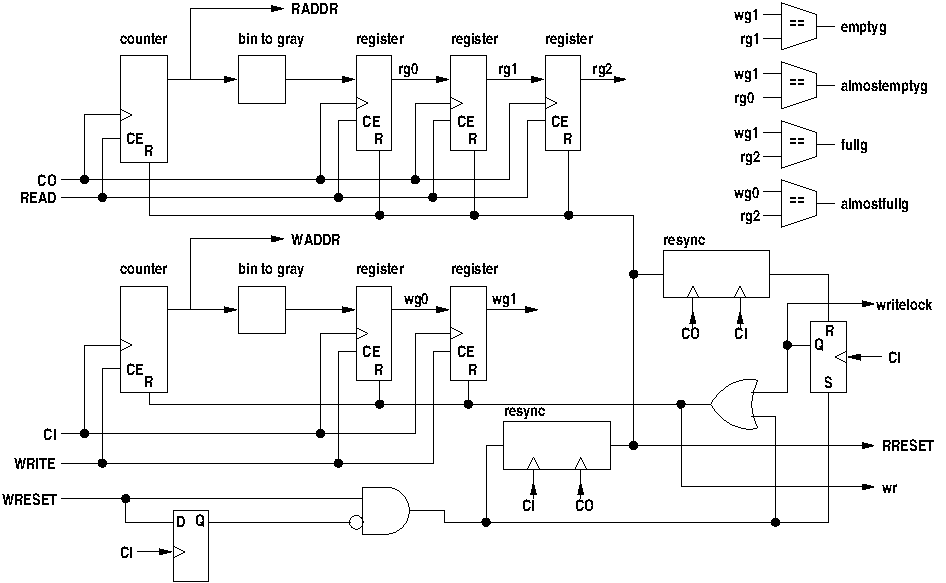
\includegraphics{asyncaddr}

        When {\bf WRESET} is asserted it resets the write address
        counter to zero and the following grey code registers
        to the initial values -

        \begin{tabular}{c c}
        wg0 & 100...000 \\
        wg1 & 100...001 \\
        \end{tabular}

        At the same time it is gated through to {\bf FULL} and
        also latched in a flip-flop so that
        the queuebuffer appears full and will not be written on the
        current or subsequent clock cycles. The write reset is
        resynchronised to the read clock and the resulting signal
        is output to {\bf RRESET} for possible daisy chaining to
        further queues in the pipeline. {\bf RRESET} also resets the
        {\bf EMPTY} flip-flop,
        resets the read address counter to zero and the following
        grey code registers to the initial values -

        \begin{tabular}{c c}
        rg0 & 100...000 \\
        rg1 & 100...001 \\
        rg2 & 100...011 \\
        \end{tabular}

        These initial values on the write and read sides ensure the queue
        buffer appears initially empty and empty after a reset. The
        values are the gray code sequence leading up to the current read
        and write addresses of 0 (gray code 0) and hence are gray code
        equivalents of -1, -2 and -3.

        {\bf RRESET} is then resynchronised back to the write
        clock and resets the flip-flop holding {\bf FULL} asserted.
        The reset process thus takes a number of read and write
        clock cycles, the exact duration depending on the two clock
        frequencies. The reset inhibits any writes on the current
        clock cycle and from then on until the reset is complete.
        The queue buffer does not appear empty immediately the
        reset is asserted on the write side, however only one read
        can take place (if the queue buffer is not already empty) and
        that will read a correct datum. After that the queue buffer
        will be reset on the read side and will appear empty. The
        queue buffer can then only appear non-empty after a
        subsequent write following the reset.

        The gray code address comparisons at various phases are
        compared to determine empty and full conditions -

        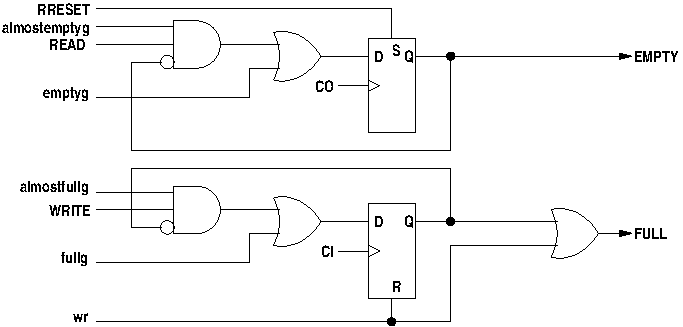
\includegraphics{asyncfullempty}

        The binary to gray code converter logic is -

        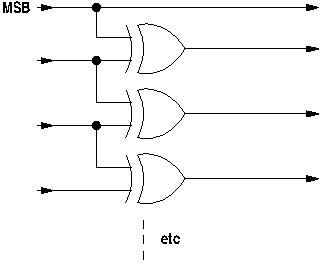
\includegraphics{bintogray}

        which is coded as -
        \begin{lstlisting}[gobble=8, language=java]
            private Net[] bin_to_gray (Net[] in) {
                int     size = in.length;
                Net[]   out = new Net[size];

                out[size-1] = in[size-1];
                for (int i=size-2 ; i>=0 ; i--)
                    out[i] = XOR(in[i+1], in[i]);
                return(out);
        }
        \end{lstlisting}

        The asynchronous control logic in method
        asynch\_fifo\_control() is coded as -
        \begin{lstlisting}[gobble=8, language=java]
            private void asynch_fifo_control (
                Net write, Net ne, Net pop, Net wc, Net rc, Net r,      // input nets
                Net[] waddr, Net[] raddr,                               // output nets
                Net[] rstat, Net[] wstat, Net full, Net empty, Net rr,  // output nets
                int awidth, int depth
                // write is the write enable
                // ne is true if the asynchronous FIFO is not empty
                // pop is true to pop a datum
                // wc is the write clock
                // rc is the read clock
                // r is a reset synchronised to the write clock or null
                // waddr is the write address
                // raddr is the read address     
                // rstat is the read buffer status
                // wstat is the write buffer status
                // full is the net to return the full condition
                // empty is the net to return the empty condition
                // rr is a reset synchronised to the read clock
                // awidth is the address width
                // depth is the FIFO depth
            ) {
                Net[]   wg0, wg1, rg0, rg1, rg2;
                Net     emptyg, almostemptyg, fullg, almostfullg;
                Net     wr = null;  // extended write reset
                Net     writelock = null;
                Net     read;
                // Initial gray code values of pipelined read and write address registers.
                // These are address sequences leading up to the initial read and
                // write addresses of 0, hence they are gray code values of -1, -2 and -3.
                String  igm1 = intToGrayString(-1, awidth);
                String  igm2 = intToGrayString(-2, awidth);
                String  igm3 = intToGrayString(-3, awidth);

                if ((r != null) && r.isConnected(Net.LO))
                    r = null;
                if (r != null) {
                    r = AND(r, INV(FDRS(r, wc, null, null, null, null, null)));
                    rr.connect(resync(r, wc, rc));
                    writelock = FDRS(null, wc, null, resync(rr, rc, wc), r, "R", null);
                    wr = OR(r, writelock);
                } else if (rr != null)
                    rr.connect(Net.LO);

                read = AND(OR(INV(ne), pop), INV(empty));

                connect(raddr, cb(awidth, false, rc, read, rr, null, null));
                rg0 = reg(bin_to_gray(raddr), rc, read, rr, igm1, null);
                rg1 = reg(rg0, rc, read, rr, igm2, null);
                rg2 = reg(rg1, rc, read, rr, igm3, null);

                connect(waddr, cb(awidth, false, wc, write, wr, null, null));
                wg0 = reg(bin_to_gray(waddr), wc, write, wr, igm1, null);
                wg1 = reg(wg0, wc, write, wr, igm2, null);

                emptyg       = eq(wg1, rg1, false, false);
                almostemptyg = eq(wg1, rg0, false, false);
                fullg        = eq(wg1, rg2, false, false);
                almostfullg  = eq(wg0, rg2, false, false);
                Net empty_d;
                if (lutwidth >= 5)
                    empty_d = OR(AND(OR(INV(ne), pop), INV(empty), almostemptyg), emptyg);
                else {
                    Net n = AND(OR(INV(ne), pop), INV(empty), almostemptyg);
                    empty_d = MUXF5(emptyg, n, Net.HI);
                }
                empty.connect(FDRS(empty_d, rc,  null, null, rr, "S", null));
                if (r != null) {
                    Net full_;
                    full_ = FDRS(OR(fullg, AND(almostfullg, write, INV(full))), wc, null, wr, null, "R", null);
                    full.connect(OR(full_, wr));
                } else
                    full.connect(FDRS(OR(fullg, AND(almostfullg, write, INV(full))), wc, null, null, null, "R", null));

                if ((rstat != null) || (wstat != null)) {
                    Net[]   rgtop, wgtop;
                    rgtop = new Net[2];
                    wgtop = new Net[2];
                    rgtop[0] = rg1[awidth-2];
                    rgtop[1] = rg1[awidth-1];
                    wgtop[0] = wg1[awidth-2];
                    wgtop[1] = wg1[awidth-1];
                    if (rstat != null)
                        asynch_fifo_control_status(rstat, rgtop, wgtop, rc, rr);
                    if (wstat != null)
                        asynch_fifo_control_status(wstat, rgtop, wgtop, wc, wr);
                }
            }
        \end{lstlisting}

        Method {\bf asynch\_fifo\_control\_status()}, which is called if
        the read status ({\bf rstat}) or write status ({\bf wstat})
        arguments are non-null, generates logic to return the buffer
        occupancy status. This status gives an approximate view, the
        asynchronous nature of the queue buffer precluding actual
        occupancy counts.

        \begin{lstlisting}[gobble=8, language=java]
            private void asynch_fifo_control_status (Net[] stat, Net[] rgtop, Net[] wgtop, Net c, Net r) {
                Net n, n1, n2, n3, n4;
                // Empty to 1/4 Full - quads equal
                n = AND(eq(rgtop, wgtop, false, false), INV(OR(stat[3], stat[4])));
                stat[0].connect(FDRS(n, c,  null, null, r, "S", null));
                // 1 word to 1/2 Full - quad 1 ahead
                n1 = AND(decode(rgtop, 0), decode(wgtop, 1));
                n2 = AND(decode(rgtop, 1), decode(wgtop, 3));
                n3 = AND(decode(rgtop, 3), decode(wgtop, 2));
                n4 = AND(decode(rgtop, 2), decode(wgtop, 0));
                n = OR(n1, n2, n3, n4);
                stat[1].connect(FDRS(n, c, null, r, null, "R", null));
                // 1/4 full to 3/4 Full - quad 2 ahead
                n1 = AND(decode(rgtop, 0), decode(wgtop, 3));
                n2 = AND(decode(rgtop, 1), decode(wgtop, 2));
                n3 = AND(decode(rgtop, 3), decode(wgtop, 0));
                n4 = AND(decode(rgtop, 2), decode(wgtop, 1));
                n = OR(n1, n2, n3, n4);
                stat[2].connect(FDRS(n, c, null, r, null, "R", null));
                // 1/2 Full to Full - quad 3 ahead
                n1 = AND(decode(rgtop, 0), decode(wgtop, 2));
                n2 = AND(decode(rgtop, 1), decode(wgtop, 0));
                n3 = AND(decode(rgtop, 3), decode(wgtop, 1));
                n4 = AND(decode(rgtop, 2), decode(wgtop, 3));
                n = OR(n1, n2, n3, n4);
                stat[3].connect(FDRS(n, c, null, r, null, "R", null));
                // 3/4 Full to Full - quad 4 ahead/equal
                n = AND(eq(rgtop, wgtop, false, false), OR(stat[3], stat[4]));
                stat[4].connect(FDRS(n, c, null, r, null, "R", null));
            }
        \end{lstlisting}




    \subsubsection{triggerbuffer()}

        This method creates a synchronous or asynchronous queue buffer
        that has only the control logic and no actual data buffer.
        The code is just the control logic taken from
        methods {\bf sync\_buffer()} and {\bf async\_buffer()}.


    \subsubsection{queueunbuffered()}
    
        A synchronous unbuffered queue is not really a queue and hence
        the control inputs and outputs are labelled differently to
        a buffered queue -
        
        \begin{tabular}{l l}
        buffered & unbuffered\\
        \\
         NE     & ravail  \\
         NF     & wavail  \\
         PUSH   & wpending\\
         POP    & rpending\\
        \end{tabular}

        A synchronous unbuffered queue is created by connecting the {\bf ravail}
        output net to the {\bf wpending} input net and the {\bf wavail} output
        net to the {\bf rpending} input net. With these cross connections
        asserting the {\bf wpending} input asserts the {\bf ravail} output and
        the queue now has read availability. In the same way asserting the {\bf
        rpending} input asserts the {\bf wavail} output and the queue now
        exhibits write availability. These cross connections are valid because
        wpending implies a write is ready to proceed and that a read can now be
        made. Similarly rpending implies that  read is ready to proceed and
        hence a write can now be executed. The rpending and wpending logic
        cannot be driven from the {\bf START\_DEL} output of two EXECPs as for a
        buffered queue as these are not asserted until the availability outputs
        are asserted. This circular logic will deadlock. Instead the {\bf
        wpending} and {\bf rpending} inputs are driven by the {\bf PENDING}
        output of EXECPs. This has been described previously (\ref{ubqueuerw}). The data
        output is simply connected to the data input as the unbuffered queue
        does not store anything.

        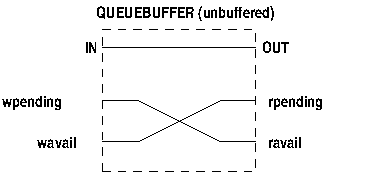
\includegraphics{ubqueue}

        \begin{lstlisting}[gobble=8, language=java]
            ravail.connect(wpending);
            wavail.connect(rpending);
            return(in);
        \end{lstlisting}

        Asynchronous unbuffered queues are not implemented.



    \subsubsection{queuefifo()}
    
        For synchronous queues created by {\bf sync\_buffer()} or asynchronous
        queues created by {\bf async\_buffer()}, if the FPGA is Virtex 5, Virtex 6
        or system7 and the depth is less than 8192 and the fifo attribute has been
        set on the queue, then methid {\bf queuefifo()} will be called. This will in
        turn call {\bf fifallocate()} in the FPGA class. This in turn will
        construct a list of {\bf FifoBlock} instances to the required width and
        then call method FIFO() in class {\bf FifoBlock} on each to construct the
        block RAM FIFOs.



\subsection{delay line}

    \begin{lstlisting}[gobble=4, language=java]
        public Net[] del (
            int         n,      // line length
            Net[]       in,     // input net array
            Net[]       len,    // optional variable length selection input
            Net         c,      // clock
            Net         ce,     // optional clock enable
            Net         r,      // optional reset
            ArrayList   init    // initial delay line contents as a list of
                                // hexadecimal strings
        ) {
            if ((n == 0) && (len == null))
                return(in);

            int             blklen = 1 << srladdrwidth;
            int             width = in.length;
            Net[]           out = new Net[width];
            boolean         flip_flops = (n == 1) || ((r != null) && (!r.isConnected(Net.LO)));
            boolean         varlen = (len != null);
            StringBuffer    binit = null;
            int             del_len;

            if (varlen)
                n = blklen;

            for (int k=0 ; k<width ; k++) {
                // if delay of only 1 use flip-flop
                // if reset input is used, must use flip-flops
                if (flip_flops) {
                    Net[]   s = new Net[n+1];
                    s[0] = in[k];
                    for (int i=0 ; i<n ; i++)
                        if ((init == null) || strhexbit((String)init.get(i), k) == 0)
                            s[i+1] = FDRS(s[i], c, ce, r, null, "R", null);
                        else
                            s[i+1] = FDRS(s[i], c, ce, null, r, "S", null);
                    out[k] = s[n];
                    continue;
                }

                // use delay lines
                String sinit;
                if (init != null) {
                    binit = new StringBuffer();
                    for (int i=0 ; i<n ; i++) {
                        int b = strhexbit((String)init.get(i), k);
                        binit.insert(0, (b == 0) ? "0" : "1");
                    }
                    sinit = binToHex(binit);
                } else
                    sinit = "0";
                if (varlen) {
                    // variable length
                    switch (srladdrwidth) {
                    case 4:
                        out[k] = SRL16E(in[k], c, ce, len, sinit, null);
                        break;
                    case 5:
                        out[k] = SRL32E(in[k], c, ce, len, sinit, false, null);
                    }
                } else {
                    // Constant length.
                    // Insert a flip-flop at the output to improve timing,
                    // so use n-1 as length.
                    int     blocks = (n - 2) / blklen + 1;
                    Net[]   s = new Net[blocks+1];
                    boolean q31;
                    int     ffinit = 0;
                    if ((binit != null) && (binit.charAt(binit.length() - n) == '1')) {
                         // remove 1 bit - used with flip-flop
                        ffinit = 1;
                        binit.deleteCharAt(binit.length() - n);
                    }
                    len = new Net[srladdrwidth];
                    s[0] = in[k];
                    for (int i=0, count=n-1 ; i<blocks ; i++, count-=blklen) {
                        int m = (count < blklen) ? count-1 : blklen-1;
                        for (int j=0 ; j<srladdrwidth ; j++)
                            len[j] = (((m >> j) & 1) == 1) ? Net.HI : Net.LO;
                        if (binit != null)
                            sinit = binToHex(binit);
                        switch (srladdrwidth) {
                        case 4:
                            s[i+1] = SRL16E(s[i], c, ce, len, stringsize(sinit, srladdrwidth), null);
                            break;
                        case 5:
                            q31 = (i != (blocks - 1));
                            s[i+1] = SRL32E(s[i], c, ce, len, stringsize(sinit, srladdrwidth), q31, null);
                        }
                        del_len = 1 << srladdrwidth;
                        if (binit != null) {
                            if (binit.length() >= del_len)
                                binit.delete(binit.length() - del_len, binit.length());
                            else
                                binit.delete(0, binit.length());
                        }
                    }

                    if ((init == null) || ffinit == 0)
                        out[k] = FDRS(s[blocks], c, ce, r, null, "R", null);
                    else
                        out[k] = FDRS(s[blocks], c, ce, null, r, "S", null);
                }
            }
            return(out);
        }
    \end{lstlisting}

    A delay line can be fixed or variable length and may be initialised.
    An initialised delay line with feedback can be used to generate a
    sequence. The parameter {\bf init} is a list of hexadecimal strings,
    one per delay line stage, i.e. each string is a value across the
    width of the delay line.

    Variable {\bf blklen} is the length of an SRL shift register (16 or
    32 depending on FPGA). If the delay line is to have variable length
    ({\bf varlen} is true) it is limited to a maximum of blklen (line
    21).

    Variable {\bf flip\_flops} is true if the delay line length is 1 or if
    the reset {\bf r} is non-null and is not tied false. If true, flip-flops
    will be used to construct the delay line rather than CLB shift registers
    (shift registers cannot be reset).

    The outer loop starting at line 22 takes each bit of the data width
    in turn.

    If {\bf flip\_flops} is true (line 25) flip-flops are used for the
    delay line. The inner loop starting at line 28 iterates along the
    length of the delay line creating an FDRS for each bit. The FDRS is
    initialised by extracting the matching bit from the initialisation
    string and either the {\bf R} or {\bf S} input is connected to net
    {\bf r} as appropriate. On completion of the inner loop the
    continue statement skips to line 98 to continue the outer loop.

    Where shift CLB registers are used ({\bf flip\_flops} is false)
    the initialisation data must be transposed as the SRL registers
    run lengthwise. This is done into variable {\bf sinit}. If the
    shift register is variable length then a single SRL16 or SRL32
    is created. The net array {\bf len} is the address input to select
    the length of the line dynamically.

    If the length of the line is fixed then SRL16 or SRL32 elements are
    concatenated in the loop starting at line 71 to get the required
    line length. The data inputs, data outputs, line length and
    initialisation data are all segmented to match the concatenated
    elements. Note that the final unit of the delay line is implemented
    using flip-flops. This is done because the output-to-clock delay of
    an SRL16 or SRL32 is quite long and this can cause problems with
    timing constraints. The addition of a trailing flip-flop alleviates
    this problem. Note that a variable length line cannot have trailing
    flip-flops (unless a minimum delay of 2 were acceptable) and hence
    may experience timing constraint problems.


\subsection{shifters}

    Left and right fixed shift is performed by methods {\bf lshift()}
    and {\bf rshift()}. These generate no logic and simply connect
    the output net array to the input net array with a displacement.
    Padding to GND is done to outputs shifted off-end except in the
    case of signed most significant bits which are connected to the
    input MSB (sign bit).

    Variable shift is performed by method {\bf var\_shift3pl()}.
    \begin{lstlisting}[gobble=4, language=java]
        public Net[] var_shift3pl (
            Net[]   a,      // input argument - signed or unsigned
            Net[]   s,      // shift argument - unsigned
            int     owidth, // output bit width
            boolean right,  // true for right shift, false for left shift
            boolean signeda // true if the input is signed
        ) {
            int     iwidth = a.length;
            int     shiftsize = s.length;
            int     shiftbits = (1 << shiftsize) - 1;
            long    ssize = Math.min(shiftbits, owidth);
            int     shiftdim = bits(ssize, false);  
            Net[]   shift = new Net[shiftdim];
            int     stages = shiftdim;
            Net[][] v = new Net[stages+1][owidth];
            Net     p1, p2;
            Net[]   o = new Net[owidth];
            int     i, j, k, l, l1, l2;

            if (right) {
                if (signeda)
                    p1 = a[iwidth-1];
                else
                    p1 = Net.LO;
                p2 = Net.LO;

            } else {
                if (signeda)
                    p2 = a[iwidth-1];
                else
                    p2 = Net.LO;
                p1 = Net.LO;
            }

            // prune the shift array to match the output width if too big
            shift = subarray(s, 0, shiftdim-1);

            for (i=0 ; i<iwidth ; i++)
                if (right)
                    // reverse input bit order for right shift
                    v[0][i] = a[iwidth-i-1];
                else
                    v[0][i] = a[i];

            k = iwidth;
            for (j=1 ; j<=stages ; j++) {
                k = Math.min(owidth, iwidth + (1 << j) - 1);
                l = iwidth + (1 << (j-1)) - 1;
                for (i=0 ; i<k ; i++) {
                    l1 = i - (1 << ( j - 1));
                    l2 = i;
                    if (l1 < 0)
                        v[j][i] = mux2(shift[j-1], v[j-1][l2], p1);
                    else if (l2 >= l)
                        v[j][i] = mux2(shift[j-1], p2, v[j-1][l1]);
                    else
                        v[j][i] = mux2(shift[j-1], v[j-1][l2], v[j-1][l1]);
                }
            }

            for (i=0 ; i<owidth ; i++)
                if (right)
                    // reverse output bit order for right shift
                    o[owidth-i-1] = v[stages][i];
                else
                    o[i] = v[stages][i];
            return(o);
        }
    \end{lstlisting}

    This constructs a variable left shift and simply reverses both input
    and output arrays for a right shift. The shift is unsigned so it
    cannot be negative. The shift is accomplished by successive stages
    of multiplexers which select either unshifted bits or bits shifted
    by a power of 2. Each stage is controlled by one bit of the shift
    value. Note that the extra width of the output array (over that of
    the input array) is handled differently depending on whether the
    shift is left or right. The output width is determined in
    constructor nodes.ArgParams() called from nodes.ExprNode.getVal()
    and depends on the input type. For a signed or unsigned integer
    the width is expanded for left shift but not for right shift. Thus
    for right shift the bits shifted off end are lost. For fixed point
    types right shift bits are retained within the fractional part
    of the word but are lost beyond that. Where the output array is
    smaller than the output array of the shifter, {\bf v[stages][]},
    the output array is assigned at the lower subscript end and the
    higher subscript bits are not connected.
    The resulting logic is illustrated by the following diagram
    for the case of 8-bit input and a 3-bit shift value -

    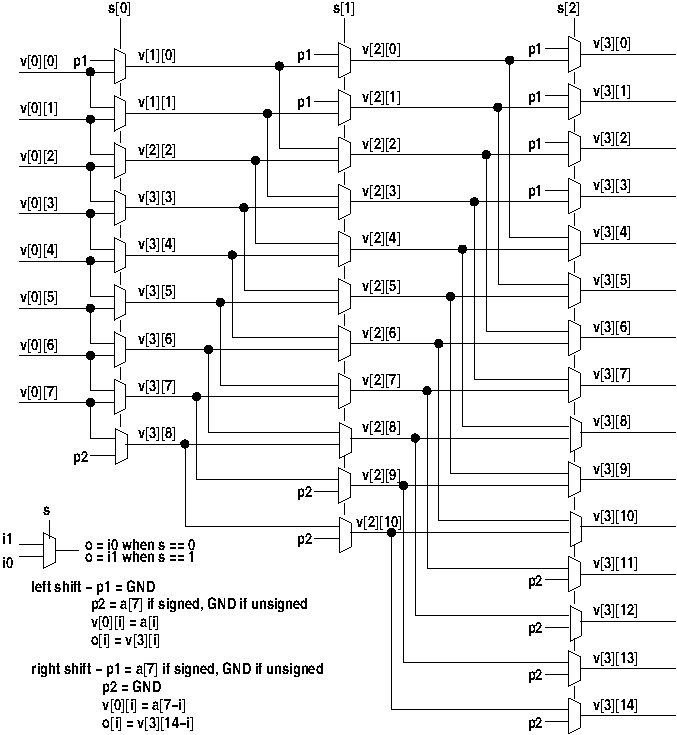
\includegraphics{vshift}


\subsection{adder}


    \begin{lstlisting}[gobble=4, language=java]
        public Net[] add (Net[] a, Net[] b, boolean asigned, boolean bsigned, int osize) {
            int     awid = a.length + ((!asigned && bsigned) ? 1 : 0);
            int     bwid = b.length + ((asigned && !bsigned) ? 1 : 0);
            int     isize = Math.max(awid, bwid);

            if (osize == 0)
                osize = isize + 1;

            Net[]   ps = new Net[osize];    // partial sum
            Net[]   s = new Net[osize];     // sum
            Net[]   c = new Net[osize];     // carries

            a = sig_expand(a, osize, asigned);
            b = sig_expand(b, osize, bsigned);

            int i = 0;

            // Starting at the LSB, while either operand is GND simply copy
            // the other operand to the output. When neither is GND, exit
            // the loop and proceed to normal addition logic for the rest of the
            // bits.
            for ( ; i<osize ; i++) {
                if (a[i].isConnected(Net.LO))
                    s[i] = b[i];
                else if (b[i].isConnected(Net.LO))
                    s[i] = a[i];
                else
                    break;
            }
            if (i < osize)
                c[i] = Net.LO;  // start carry chain if adder still needed

            // Adder stages (if required; i < size).
            int ilast = osize - 1;
            if (!needCPLDarith()) {
                // FPGAs
                for ( ; i<osize ; i++) {
                    if (add_sub_use_lut)
                        ps[i] = LUT("I0^I1", a[i], b[i]);
                    else
                        ps[i] = XOR(a[i], b[i]);
                    s[i] = XORCY(ps[i], c[i]);
                    if (i != ilast)
                        c[i+1] = MUXCY(ps[i], a[i], c[i]);
                }
            } else {
                // CPLDs
                for ( ; i<osize ; i++) {
                    if (cpld_use_lut)
                        s[i] = LUT("I0^I1^I2", a[i], b[i], c[i]);
                    else
                        s[i] = OR(  AND(    a[i],  INV(b[i]), INV(c[i])),
                                    AND(INV(a[i]),     b[i],  INV(c[i])),
                                    AND(INV(a[i]), INV(b[i]),     c[i]),
                                    AND(    a[i],      b[i],      c[i])   );
                    if (i != ilast) {
                        if (cpld_use_lut)
                            c[i+1] = LUT("I0*I1*!I2+I0*!I1*I2+!I0*I1*I2+I0*I1*I2",
                                                                a[i], b[i], c[i]);
                        else
                            c[i+1] = OR(    AND(    a[i],      b[i], INV(c[i])),
                                            AND(    a[i],  INV(b[i]),    c[i]),
                                            AND(INV(a[i]),     b[i],     c[i]),
                                            AND(    a[i],      b[i],     c[i])  );
                    }
                }
            }

            return(s);
        }
    \end{lstlisting}

    This creates an adder. The input nets may be different sizes. The
    output net is one larger than the largest input net. The MSB of
    the result is the final carry bit.

    If the bits of one operand starting from the least significant end
    are a sequence of zeros (GND) then those adder stages are omitted
    and corresponding bits from the other operand become the sum
    bits. The adder stages are constructed from this point onwards
    (note that the for loops do not initialise loop variable {\bf i}
    which remains at the point the input constant search finished).
    If the two operands do not have overlapping variable bits then
    the extra top bit is set appropriately (0 or one of the signs)
    and no adder stages are constructed (i == size so the following
    for loops do not execute).

    For FPGAs the carry chain is used.

    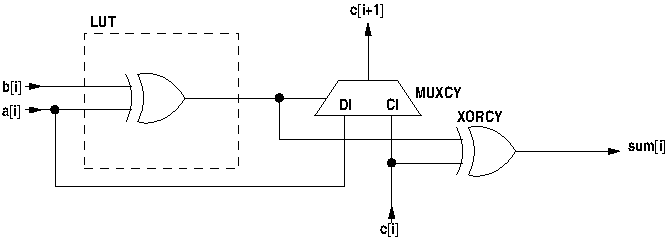
\includegraphics{add}

    If {\bf needCPLDarith()} returns true then the adder is constructed
    only from LUT logic because there is no carry chain available.

    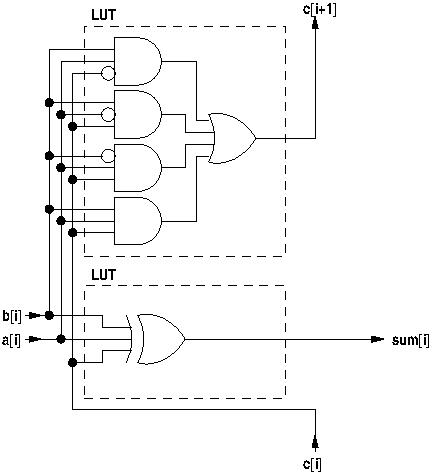
\includegraphics{add_ncc}

    The variables {\bf add\_sub\_use\_lut} and {\bf cpld\_use\_lut} are public
    static variables in ThreePL.jj and select whether the combinatorial
    logic is expressed as a LUT or a combination of AND, OR, XOR and
    INV elements. While the boolean logic is identical the ability of
    the place-and-route tools to optimise the logic may be affected
    by the choice. By default these variables are true to select
    encoding as LUTs. The {\bf -G} option to 3PL renders these
    variables (and many similar ones in other methods) false.



\subsection{inverter}

    The code to create a 1's complement inverter is trivial.


\subsection{incrementer}

    The incrementer method is only used for signed division (method {\bf
    part\_sdiv(})) and for an up/down counter ({\bf method cb()}). It is
    derived from the code for method {\bf add()} with the second input
    {\bf b} omitted and the carry input connected to an {\bf enable}
    input. Thus when {\bf enable} is low the output is the same as the
    input {\bf a} and when {\bf enable} is high the output
    is {\bf a} + 1. The result is the same width as the input, not one
    greater.


\subsection{subtracter}

    \begin{lstlisting}[gobble=4, language=java]
        public Net[] sub (Net[] a, Net[] b, boolean asigned, boolean bsigned, int osize) {
            int     awid = a.length + ((!asigned && bsigned) ? 1 : 0);
            int     bwid = b.length + ((asigned && !bsigned) ? 1 : 0);
            int     isize = Math.max(awid, bwid);

            if (osize == 0)
                osize = isize + 1;

            Net[]   pd = new Net[osize]; // partial difference
            Net[]   d = new Net[osize];  // difference
            Net[]   c = new Net[osize];  // carries

            a = sig_expand(a, osize, asigned);
            b = sig_expand(b, osize, bsigned);

            int i = 0;

            // Starting at the LSB, while 2nd operand is GND simply copy
            // the 1st operand to the output. When 2nd operand is no
            // longer GND, exit the loop and proceed to normal subtraction
            // logic for the rest of the bits. 2nd operand should never be
            // all zeros as the subtraction would have been optimised out
            // prior to this.
            for ( ; i<osize ; i++) {
                if (b[i].isConnected(Net.LO))
                    d[i] = a[i];
                else
                    break;
            }
            c[i] = Net.HI;

            int ilast = osize - 1;
            if (!needCPLDarith()) {
                // FPGAs
                for ( ; i<osize ; i++) {
                    if (add_sub_use_lut)
                        pd[i] = LUT("I0^!I1", a[i], b[i]);
                    else
                        pd[i] = XOR(a[i], INV(b[i]));
                    d[i] = XORCY(pd[i], c[i]);
                    if (i != ilast)
                        c[i+1] = MUXCY(pd[i], a[i], c[i]);
                }
            } else {
                // CPLDs
                for ( ; i<osize ; i++) {
                    if (cpld_use_lut)
                        d[i] = LUT("I0^!I1^I2", a[i], b[i], c[i]);
                    else
                        d[i] = OR(  AND(    a[i],      b[i],   INV(c[i])),
                                    AND(INV(a[i]), INV(b[i]),  INV(c[i])),
                                    AND(INV(a[i]),     b[i],       c[i]),
                                    AND(    a[i],  INV(b[i]),      c[i])   );
                    if (i != ilast)
                        if (cpld_use_lut)
                            c[i+1] = LUT("I0*!I1*!I2+!I0*!I1*I2+I0*I1*I2+I0*!I1*I2",
                                                                a[i], b[i], c[i]);
                        else
                            c[i+1] = OR(    AND(    a[i],  INV(b[i]), INV(c[i])),
                                            AND(    a[i],      b[i],      c[i]),
                                            AND(INV(a[i]), INV(b[i]),     c[i]),
                                            AND(    a[i],  INV(b[i]),     c[i])  );
                }
            }
            return(d);
        }
    \end{lstlisting}

    The input operands are expanded to the size of the largest of the
    two plus one to match the required size of the difference.

    If the bits of the second operand starting from the least
    significant end are a sequence of zeros (GND) then those subtracter
    stages are omitted and corresponding bits from the other operand
    become the difference bits. The subtracter stages are constructed
    from this point onwards (note that the for loops do not initialise
    loop variable {\bf i} which remains at the point the input constant
    search finished).

    For FPGAs the carry chain is used.

    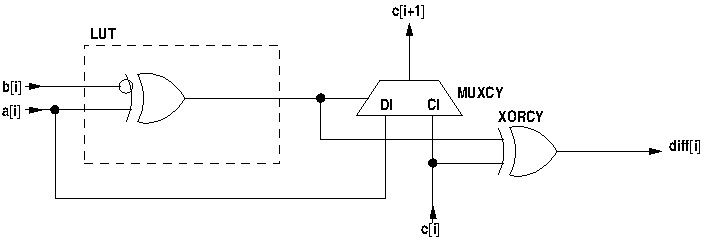
\includegraphics{sub}

    If {\bf needCPLDarith()} returns true then the adder is constructed
    only from LUT logic because there is no carry chain available.

    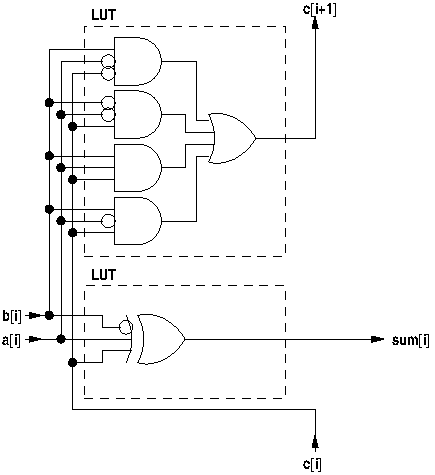
\includegraphics{sub_ncc}

    As in the case of {\bf add(}) the variables {\bf add\_sub\_use\_lut}
    and {\bf cpld\_use\_lut}, which are public static variables in
    ThreePL.jj, select whether the combinatorial logic is expressed
    as a LUT or a combination of AND, OR, XOR and INV elements.

\subsection{decrementer}

    The decrementer method is only used for an up/down counter ({\bf
    method cb()}). It is derived from the code for method {\bf sub()}
    with the second input {\bf b} omitted and the carry input connected
    to the inverted {\bf enable} input. Thus when {\bf enable} is low the output
    is the same as the input {\bf a} and when {\bf enable} is high the
    output is {\bf a} - 1. The result is the same width as the input,
    not one greater.

    {\bf Warning} - method {\bf cb()} only calls {\bf decr()} if its
    sixth parameter {\bf down} is not null and its second parameter {\bf
    dwn} is true. This does not occur in the code as it currently is and
    hence {\bf decr()} has never been called and its validity has not
    been tested!


\subsection{adder/subtracter}

    This adder/subtracter is used internally in XFunctions.java for the
    implementation of division. It is also used for the inbuilt
    function {\bf addsub()} (called in XTDECode.java.TDEOPERATOR()).
    It provides the ability to gate the second operand so that the
    add/subtract is supressed and it XORs the carry input with an
    input Net so that the carry input can be inverted. For addition
    this will increment the sum with no extra logic.

    \begin{lstlisting}[gobble=4, language=java]
        public Net[] addsub (Net[] a, Net[] b, Net add, Net igb, Net xci, boolean asigned, boolean bsigned) {
            if (needCPLDarith())
                    throw new ExEx("CPLD CODE ERROR - addsub() used");

            int     awid = a.length + ((!asigned && bsigned) ? 1 : 0);
            int     bwid = b.length + ((asigned && !bsigned) ? 1 : 0);
            int     size = Math.max(awid, bwid) + 1;
            Net[]   di = new Net[size];
            Net[]   psd = new Net[size]; // partial sum/difference
            Net[]   sd = new Net[size];  // sum/difference
            Net[]   c = new Net[size];   // carries

            a = sig_expand(a, size, asigned);
            b = sig_expand(b, size, bsigned);
            if (xci.isConnected(Net.LO))
                c[0] = AND(INV(add), igb);
            else
                c[0] = AND(XOR(INV(add), xci), igb);
            for (int i=0 ; i<size ; i++) {
                if (igb.isConnected(Net.LO))
                    psd[i] = a[i];
                else if (igb.isConnected(Net.HI)) {
                    if (add.isConnected(Net.LO))
                        psd[i] = XOR(a[i], INV(b[i]));
                    else if (add.isConnected(Net.HI))
                        psd[i] = XOR(a[i], b[i]);
                    else
                        psd[i] = OR(AND(add, XOR(a[i], b[i])), AND(INV(add), XOR(a[i], INV(b[i]))));
                } else {
                    if (add_sub_use_lut)
                        psd[i] = LUT("(!I0*I1)+(I0*(I3*(I1^I2)+!I3*(I1^!I2)))", igb, a[i], b[i], add);
                    else
                        psd[i] = OR(    AND(INV(igb), a[i]),
                                        AND(igb, OR(    AND(add, XOR(a[i], b[i])),
                                                        AND(INV(add), XOR(a[i], INV(b[i]))))));
                }
                if (igb.isConnected(Net.LO))
                    di[i] = Net.LO;
                else if (igb.isConnected(Net.HI))
                    di[i] = a[i];
                else
                    di[i] = MULT_AND(a[i], igb);
                if (i != (size-1))
                    c[i+1] = MUXCY(psd[i], di[i], c[i]);
                sd[i] = XORCY(psd[i], c[i]);
            }
            return(sd);
        }
    \end{lstlisting}

    The implementation does not provide a non-carry-chain version
    for CPLDs, hence the check on entering the method.

    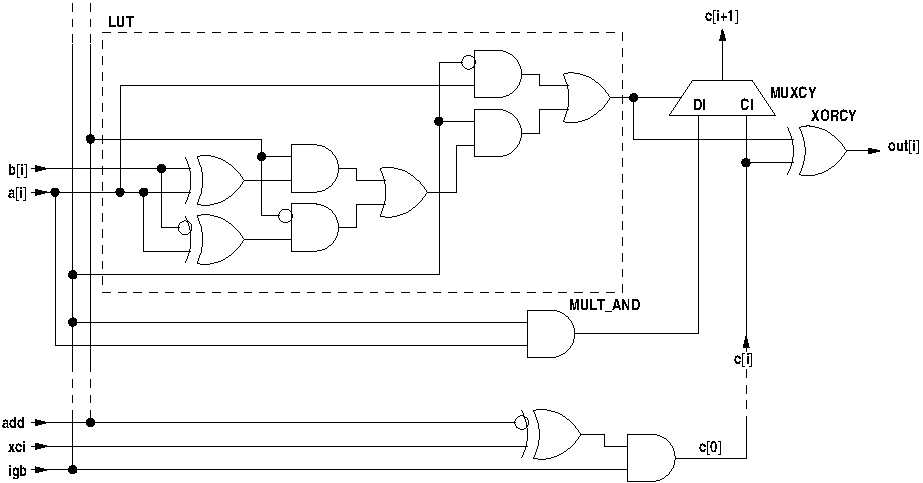
\includegraphics{addsub}

    Note that if {\bf igb} is low {\bf a[i]} is passed through the LUT
    and the XORCY unchanged. The LUT function passes a[i] through to
    its output and the XORCY has a low from the carry on its other input.
    The carry chain is low along its length as {\bf c[0]} is forced low
    and the {\bf DI} inputs to the MUXCYs are forced low.

    The {\bf add} input inverts the {\bf b[i]} inputs and also controls
    the carry input, {\bf c[0]} (low for add, high for subtract). {\bf
    xci} inverts that {\bf c[0]} input.

    The expression represented in lines 37 and 39 and in the logic
    diagram could be written more concisely but it does not matter as it
    would be converted to the same function of four variables in the LUT
    in either case.

\subsection{ALU}

    The {\bf alu()} code is very similar to the {\bf addsub()} with
    the following exceptions -
    \blist
    \item   the {\bf xci} input and function is omitted
    \item   it has an {\bf iga} input instead of {\bf igb}, i.e. it
            gates the {\bf a} input to give output = b when asserted
    \item   there is a {\bf dsp} parameter which if true and the device
            is a Virtex5 or later will implement the ALU in a DSP
            block instead of using CLB logic.
    \blend
    The output Net array is one larger than the largest operand.


\subsection{incrementer/decrementer}

    This method is only called in one place, method cb() in class
    XFunctions. It increments or decrements its operand according to the
    second argument. It is derived from method {\bf addsub()}. The
    output Net array is the same size as the operand (first argument).


\subsection{signed and unsigned multipliers}

    The multiplier method, {\bf mul()}, is divided into four sections
    depending on FPGA type -
    \blist
    \item   XC3S, XC2V or XC2VP
    \item   XC4V
    \item   XC5V or XC6V
    \item   others
    \blend

    This method must be called such that if the operands are of
    different sizes the first must be the larger except in the case
    where one operand is a constant in which case the constant operand
    is the second one.

    For Spartan 3, Virtex 2 or Virtex 2 Pro the MULT18X18 is used. Up to
    four multipliers can be combined to give a maximum of 35 by 35 bits
    signed (See Xilinx application note XAPP467 and Xilinx white paper
    WP277). Since the MULT18X18 performs signed multiplication, unsigned
    operands cannot use the top bit, which must be 0 to give a positive
    sign. For this reason operand size checks are different for signed
    and unsigned operands.

    For the Virtex 4 a MULT18X18 is created but this will later be
    converted to a DSP48 by the place-and-route software.

    For Virtex 5 and Virtex 6 a single MULT25X18 is used. This size
    was deemed sufficient and larger multipliers using combined
    MULT25X18 elements have not been coded.

    For other types of FPGA (Spartan 2, Virtex, Virtex E) a multiplier
    is constructed using cascaded adders. This usually results in
    considerable signal path lengths through combinatorial logic and
    hence this form of multiplier will usually only work at relatively
    low clock frequencies. All current FPGA platforms have hardware
    multipliers and this combinatorial logic is only included for
    obsolete FPGAs still in use. There is a library, {\bf multlib.3pl},
    which implements pipelined multiplies which will operate at
    high clock frequencies (which of course have multi-cycle latency).

    If the operands are mixed signed and unsigned, the unsigned operands
    has a (zero) sign bit added. If either operand is signed method {\bf
    muls()} is called, otherwise {\bf mulu()} is called. These methods
    both call method {\bf mul\_add()} for each bit of the second
    operand. If the second operand is a constant then adders are only
    created for the 1 bits and the partial product is passed on
    unchanged for 0 bits. For a constant multiplier with only a few 1
    bits the resulting multiplier will have a significantly smaller
    delay than for the case of a variable multiplier.


\subsection{signed and unsigned divider/remainder}

    Division method {\bf div()} and remainder method {\bf rem()} call the combined
    quotient/remainder method {\bf quotrem()}. {\bf quotrem()} in turn calls {\bf
    quotrems()} for signed operands or {\bf quotremu()} for usigned operands. {\bf
    quotrems()} calls recursive method {\bf part\_sdiv()} and {\bf quotremu()}
    calls recursive method {\bf part\_udiv()}. These recursive methods construct
    staged adders and subtracters to carry out the division. These stages are not
    pipelined and hence the use of division or remainder operations is likely to
    result in high path delays. These are probably not practical and have been
    included for completeness.

    
\subsection{numerical comparators}

    Methods {\bf eqones()} and {\bf eqzeros()} test for all ones and all zeros
    respectively and are implemented using AND/OR gates. For wide inputs these
    will be optimised using MUXes or carry chains.     Methods {\bf eq()} and {\bf
    ne()} compare operands and are similarly implemented to the methods above.

    Magnitude comparisons gt, ge, lt and le are all implemented using only the
    method {\bf ge()} with suitable operand order and output inversion. This is
    implemented as subtraction using the carry chain if necessary, the final carry
    bit giving the result.



\subsection{combinatorial RAM and ROM}

    Methods {\bf sram1()}, {\bf sram2()} and {\bf srom1()} build combinatorial
    RAMS (CLB RAM) of various widths and depths calling methods {\bf RAM\_1()},
    {\bf RAM\_2()} or {\bf ROM\_1()} in class XElements().


\subsection{registered output RAM}

    Methods {\bf rram1()} and {\bf rram2()} call method {\bf ramallocate()}
    in the FPGA class. This method creates a list of class RamBlock to map
    the memory across the required number of blocks and then traverses that list
    calling RamBlock.RAMB() in class RamBlock to generate the blocks elements.

    
    
    
    \section{The xilinx/XTDECode class}
    
        XTDECode extends XFunctions. Its main function is to implement the
abstract methods in class TDECode which generate netlist code from
TDEs. These methods call methods in class xilinx/XFunctions which in
turn call methods in class xilinx/XElements.

Also included in this file are methods to handle NCF (ISE) and XDC
(Vivado) constraints.




    \section{The xilinx/RamBlock class}
    
        This class provides methods to generate RAM blocks. Since the RAM
        blocks come in only a few sizes across the FPGA families the code
        is concentrated here rather than being duplicated in the various
        FPGA family classes (described earlier).

    
    \section{The xilinx/FifoBlock class}

        Thsi class provides methods to generate FIFOs based on RAM blocks
        (described earlier).











\chapter{Optimisation}

    Optimisation is carried out in the following places -

    \blist
    \item   When a TDE is added to the TDE list checks are made on
            gates and selectors for ground, VCC or duplicated inputs
            and these are optimised where appropriate. The result may be
            the elimination of the TDE.
    \item   After completion of immediate execution the complete TDE list
            is repeatedly traversed optimising both logic functions and
            control structures.
    \item   The TDE list is then traversed to perform optimisation specific
            to the target device.
    \item   The TDE list is again repeatedly traversed optimising both
            logic functions and control structures to remove any
            redundancies introduced by the target\_specific optimisation
            pass.
    \item   After conversion of the TDE list to an internal netlist
            structure that structure is repeatedly traversed to optimise
            the low-level logic. Some of the methods called are generic
            (in netlist/TDECode.java) and others are overridden by methods
            in subclasses (in netlist/xilinx/XTDECode.java).
    \blend
    
    
    \section{Optimisation on TDE addition}
    
        A TDE is added to the TDE list by calling method
        codegen.TDEList.addTDE(). This method initially applies method
        codegen.TDE.redundant() to the TDE and if the return value is true it
        returns without adding the TDE to the list. Method redundant() checks
        three types of TDE -

        \blist
        \item   a SELECT
        \item   an AND, OR or XOR gate TDE
        \item   a parallel WAIT TDE
        \blend
        
        \subsection{SELECT TDE optimisation}
        
            For a SELECT any GND data inputs, and associated select inputs, are
            removed if the no\_delete flag is not set\footnote{The no\_delete
            flag is set for a queue input where individual components are
            assigned rather than the whole variable. A queue by default
            guarantees that partial assignment will result in unassigned
            components being zeroed. The selector for such a queue cannot be
            eliminated as at the very least it must be able to gate the queue
            input to zero when not selected.}. If an input is removed the
            deletedinput class boolean is set true.
            
            Inputs are then scanned to find
            duplicated data sources and these are eliminated and their select
            signals ORed.
            
            If the selector now has no inputs the output is connected to GND and
            the method returns true so that the SELECT TDE is not added to the
            TDE list.
            
            If the selector now has one data input and -
            \blist
            \item   no GND inputs have been removed (the deletedinput boolean
                    false)
            \item   the no\_delete flag is false
            \item   the ALU flag is false\footnote{The ALU flag is true if the
                    selector is an input to a static variable which has the
                    ALU attribute true.}
            \blend
            the output is connected to that input and the method returns true so
            that the SELECT TDE is not added to the TDE list.
        
            The above three conditions reflect cases where the selector must
            be retained even though it has only one input as it performs a
            gating function on that single input.
            
            Note that codegen.TDE.redundant() is also called again during
            TDE list optimisation since inputs may have become connected
            or grounded in the meantime due to other optimisation. The
            deletedinput boolean will remain set if any ground inputs are
            removed during any of these calls so that the selector is not
            eliminated during later calls regardless of other optimisations.
            
        \subsection{Gate TDE optimisation}
        
            For a gate with only one input the output signal is connected to the
            input signal and the method returns true.
        
        \subsection{Parallel WAIT TDE optimisation}
        
            For a parallel WAIT with only one input the output signal is
            connected to the input signal and the method returns true.


    \section{TDE list general optimisation}
    
        Method codegen.TDEList.optimise() is called from parser.ThreePL to
        optimise the completed TDE list.
        
        The intermediate code list is optimised by repeated applications of
        the following -
        \begin{enumerate}
        \item   eliminate suitable CONNECT TDEs by merging their TDEVars.
                This is only done for -
                \blist
                \item   control signals, which are single bit and have no
                        WordSpec.
                \item   clock signals, again single bit.
                \item   complete TDEVars, i.e. the WordSpec of each is of
                        a complete variable.
                \blend
                This is performed by calling TDEVar.merge(). These merges are
                performed solely to enhance the readability of the optional
                TDE list file and they do not reduce logic resources or
                enhance performance.
        \item   Combine any {\bf EXECP}s with a common start and identical avail
                signal.
        \item   Combine any parallel {\bf DEL}s with a common start
                driving a common {\bf WAIT}.
        \item   Eliminate any {\bf DEL} in parallel with one or more EXECPs with
                a common start driving a common WAIT.
        \item   Eliminate any {\bf WAIT} that has a single input.
        \item   Eliminate any duplicate {\bf SELECT} inputs.
        \item   Find any AND or OR gates which have duplicated inputs
                and remove the duplicates. If this results in a single
                input remaining, eliminate the gate and connect
                the output to the input.
        \item   Find any {\bf INV}s with GND or VCC input and eliminate
                them, connecting the output to the inverse of the constant
                input.
        \item   Find any nested {\bf AND}, {\bf OR} or {\bf XOR} gates and
                consolidate them.
        \item   Find any control (not source code) {\bf AND} or {\bf OR} gates
                whose outputs are not connected and eliminate them.
        \item   Find any {\bf DEL}s whose outputs are not connected and
                eliminate them.
        \item   Find any WHENs which have a single {\bf DEL} in both the true
                block and the false block. Remove these and instead connect a
                single DEL from the start input to both the true block finish
                input and the false block finish input. This will result in
                an OR with identical inputs which will be eliminated by
                another optimisation iteration.
        \item   Eliminate any {\bf ILOOP}s which have the same output start
                signal and input finish signal. These infinite loops are
                empty, probably because they contain only value equivalence
                statements.
        \item   Find any {\bf ILOOP}s which have a single {\bf DEL} from the
                output start signal to the input finish signal. Replace the
                pair with a DFF whose SET input is driven by the start signal.
        \item   Find multiple {\bf DFF}s driven by a common {\bf START} and
                eliminate all but one.
        \item   Find any branch statements in which all branches, including
                the default, have a single DEL. Remove all the DELs and the
                final associated OR and replace with a single DEL from the
                start signal.
        \end{enumerate}
        
        These optimisations are repeatedly applied to the list until a pass
        makes no change.

    \section{TDE list device-specific optimisation}
    
        This optimisation is done in netlist.xilinx.XTDECode.TDEOptimise()
        which is called within codegen.TDEList.ncode() which has been
        called from parser.ThreePL.mainContinue().
        
        At the moment this performs three optimisations -
        \blist
        \item   It finds any SELECT TDEs which have an ALU flag and
                optimises them by moving any input ALU operations into a
                shared single ALU between the selector and its static, queue
                or selectvalue variable.
        \item   It finds any SELECT TDEs which have an ALU flag, have a
                single input and have not been optimised out and removes
                them, connecting the single input to the output.
        \item   For devices which have DSP blocks the ALU logic is implemented
                in the DSP block instead of using CLB logic where appropriate.
        \blend



    \section{Netlist optimisation}
    
        This optimisation is done in netlist.xilinx.XTDECode.optimise() called
        from codegen.TDEList.ncode() and consists of five phases -
        
        \blist
        \item   optimise gates - calling netlist.xilinx.XTDECode.optimisegates()
        \item   optimise output buffers - calling
                netlist.xilinx.XTDECode.optimiseOBUF()
        \item   optimise 3-state output buffers - calling
                netlist.xilinx.XTDECode.optimiseOBUFT()
        \item   remove resulting unconnected FD or INV - calling
                netlist.xilinx.XTDECode.optimisegates() 
        \item   optimise GND and VCC - calling
                netlist.TDECode.optimiseGNDandVCC()
        \blend
        
        netlist.xilinx.XTDECode.optimisegates() iterates through all elements
        selecting those with a gate type, Gtype, which is not Gtype.NONE
        (defined in interface netlist.NetConstants). According to gate type
        it selectively calls -
        \blist
        \item   netlist.TDECode.optimiseINV() - If the output is not
                connected, delete the inverter. Check for a low or high
                input. If high delete the gate, connecting the output net
                to Net.LO. If low delete the gate, connecting the output
                net to Net.HI. Check for an output which is also an INV
                (and the output does not go anywhere else), in which case
                delete both, connecting the input of the 1st to the output
                of the 2nd. If the intermediate output does go elsewhere,
                delete the 2nd inverter and connect the signals driven by
                its output to the input of the 1st inverter.
        \item   netlist.TDECode.optimiseAND() - If the output is not
                connected, delete the gate. Check for any low or high
                inputs or duplicated inputs. For high inputs, disconnect
                their nets. For any low inputs delete the gate connecting
                the output net to Net.LO. For any duplicated inputs delete
                all except one. If no inputs remain, delete the gate,
                connecting the output net to Net.LO. If one input remains,
                delete the gate, connecting the output net to the
                remaining input net. Check if the output goes only to
                another AND gate in which case eliminate this gate and add
                its inputs to the following gate.
        \item   netlist.TDECode.optimiseOR() - If the output is not
                connected, delete the gate. Check for any low or high
                inputs or duplicated inputs. For low inputs, disconnect
                their nets. For any high inputs delete the gate,
                connecting the output net to Net.HI. For any duplicated
                inputs delete all except one. If no inputs remain, delete
                the gate, connecting the output net to Net.LO. If one
                input remains, delete the gate, connecting the output net
                to the remaining input net.
        \item   netlist.TDECode.optimiseXOR() - If the output is not
                connected, delete the gate. Check for any low inputs. If
                found delete the inputs, disconnecting their nets. If no
                inputs remain, delete the gate, connecting the output net
                to Net.LO. Check for any high inputs. If found delete the
                inputs, disconnecting their nets, counting them in the
                process. If there were an odd number of deleted high
                inputs, convert the gate to XNOR. If one input remains,
                delete the gate, connecting the output net to the
                remaining input net.
        \item   netlist.TDECode.optimiseLUT() - Check a LUT for an
                unconnected output and remove if so.
        \item   netlist.xilinx.XTDECode.optimiseMUXCY() - Check a MUXCY
                for output not connected, in which case remove it. Check
                for constant S input, in which case delete the MUXCY and
                connect the output net to the appropriate input net.
                Check for inputs CI and DI both constant, in which case
                output is Net.HI, Net.LO, S or !S. Check for input CI low
                and DI connected to S, in which case output is Net.LO.
        \item   netlist.xilinx.XTDECode.optimiseMUXF() - Check a MUXF5,
                MUXF6 etc for constant S input. If so delete the MUXF and
                connect the output net to the appropriate input net. Check
                for inputs I0 and I1 both constant, in which case output is
                Net.HI, Net.LO, S or !S.
        \item   netlist.xilinx.XTDECode.optimiseXORCY() - Check an XORCY
                for an unconnected output and remove if so. If the CI input
                is Net.LO, eliminate the XORCY and connect the output net to
                the LI input. If the CI input is Net.HI, strip the XORCY,
                change it to an INV and connect the LI input as input I and
                reconnect the output.
        \item   netlist.xilinx.XTDECode.optimiseSRL() - Check an SRL for an
                unconnected output and remove if so.
        \item   netlist.xilinx.XTDECode.optimiseMULT\_AND() - Check a
                MULT\_AND for an unconnected output and remove if so. If any
                inputs are Net.LO, remove and connect output to Net.LO. If any
                inputs are Net.HI, remove the input.
        \item   netlist.xilinx.XTDECode.optimiseCLB\_RAM() - Check a
                dual-port CLB RAM for an unconnected output and remove if so.
                If data input is Net.LO and RAM is not initialised, remove and
                connect used outputs to Net.LO.
        \item   netlist.xilinx.XTDECode.optimiseBLK\_RAM() - If a data input
                is Net.LO or unconnected on both ports and the RAM is not
                initialised, disconnect both associated outputs if connected.
        \item   netlist.xilinx.XTDECode.optimiseMULT() - Optimise a
                MULT18X18, MULT18X18S, MULT25X18 or MULT25X18S. If no outputs
                are connected, eliminate the element. If all A inputs are
                Net.LO or all B inputs are Net.LO, eliminate and connect
                outputs to Net.LO. If the outputs are connected only to D
                inputs of FDRSs which all share the same C, CE and R, do not
                use S and are not initialised, eliminate the FDRSs and
                convert the element to a MULT18X18S. If the element is a
                MULT18X18S or MULT25X18S and has A inputs connected to a
                MULT18X18 or MULT25X18 and B inputs are Net.LO then combine
                the two into a single MULT18X18S or MULT25X18S.
        \item   netlist.xilinx.XTDECode.optimiseDSP48E() - Optimise a DSP48E
                which does not use the output register P.\\
                1. If the outputs are connected only to D inputs of FDRSs
                which all share the same C, CE and R, do not use S and are
                not initialised, or \\
                2. If the outputs are connected only to a MULREG \\
                eliminate the FDRSs or MULREG and change the DSP48E to use
                the output register.
        \item   netlist.TDECode.optimiseFDRS() -  If the output is not
                connected, delete the DFF. Check for R or S wired high
                and initial state to match. If so delete the DFF and
                connect the output net high or low. Check for D input
                GND or null, SET input GND or null and initial state
                low, in which case delete and connect output to GND.
        \blend
        Note that the methods in TDECode are generic while those in
        xilinx.XTDECode are vendor-specific (and internally may be
        family-specific).
        
        netlist.xilinx.XTDECode.optimiseOBUF() checks for an OBUF whose I
        input comes from an FD whose output is also used elsewhere. The FD
        is replicated and the link to the old FD is removed.
        
        netlist.xilinx.XTDECode.optimiseOBUFT() checks for an OBUFT whose T
        input comes from an FD, usually via an inverter. The FD replicated
        and the link to the old FD is removed. If there is an inverter, one
        is placed in the input to the new FD and its initial state is
        inverted and the S and R inputs are swapped. It also checks for an
        OBUFT whose I input comes from an FD whose output is also used
        elsewhere. The FD is replicated and the link to the old FD is
        removed.
        
        netlist.TDECode.optimiseGNDandVCC() checks that Net.LO (GND) and
        Net.HI (VCC) are used. If not used the element is removed.








\appendix

\chapter{Array dimensionality}

    \begin{verbatimtab}
    a type [10]uint:8 -
    \end{verbatimtab}

    \begin{verbatimtab}
        a       ->  [10]uint:8
        a[]     ->  [10]uint:8
        a[2..4] ->  [3]uint:8
        a[3]    ->  uint:8
    \end{verbatimtab}


    \begin{verbatimtab}
    a type (f1, log, f2, uint:4) -
    \end{verbatimtab}

    \begin{verbatimtab}
        a       ->  (f1, log, f2, uint:4)
        a.f1    ->  log
        a.f2    ->  uint:4
    \end{verbatimtab}

    \begin{verbatimtab}
    a type [10][5]uint:8 -
    \end{verbatimtab}

    \begin{verbatimtab}
        a       ->  [10][5]uint:8
        a[2..4] ->  [3][5]uint:8
        a[2]    ->  [5]uint:8
        a[][2]  ->  [10]uint:8
    \end{verbatimtab}

    \begin{verbatimtab}
    a type [10](f1, log, f2, uint:4) -
    \end{verbatimtab}

    \begin{verbatimtab}
        a[2..4]     -> [3](f1, log, f2, uint:4)
        a[2]        -> (f1, log, f2, uint:4)
        a[2..4].f1  -> [3]log
        a[2].f2     -> uint:4
    \end{verbatimtab}

    \begin{verbatimtab}
    a type [10][5](f1, log, f2, uint:4) -
    \end{verbatimtab}

    \begin{verbatimtab}
        a[2..4]         ->  [3][5](f1, log, f2, uint:4)
        a[][3]          ->  [10][5](f1, log, f2, uint:4)
        a[2][2..4]      ->  [3](f1, log, f2, uint:4)
        a[2..4][3]      ->  [3](f1, log, f2, uint:4)
        a[2][3]         ->  (f1, log, f2, uint:4)
        a[2..4].f1      ->  [3][5]log
        a[][3].f2       ->  [10][5]uint:4
        a[2][2..4].f1   ->  [3]log
        a[2..4][3].f2   ->  [3]uint:4
        a[2][3].f1      ->  log
    \end{verbatimtab}

    \begin{verbatimtab}
    a type [10][5](f1, log, f2, [4]uint:4) -
    \end{verbatimtab}

    \begin{verbatimtab}
        a[2..4]         ->  [3][5](f1, log, f2, [4]uint:4)
        a[][3]          ->  [10][5](f1, log, f2, [4]uint:4)
        a[2][2..4]      ->  [3](f1, log, f2, [4]uint:4)
        a[2..4][3]      ->  [3](f1, log, f2, [4]uint:4)
        a[2][3]         ->  (f1, log, f2, [4]uint:4)
        a[2..4].f1      ->  [3][5]log
        a[][3].f2       ->  [10][5][4]uint:4
        a[2][2..4].f1   ->  [3]log
        a[2..4][3].f2   ->  [3][4]uint:4
        a[2][3].f1      ->  log

        a[][].f2        ->  [10][5][4]uint:4
        a[][2..3].f2    ->  [10][3][4]uint:4
        a[1..3][].f2    ->  [3][5][4]uint:4
        a[2][2..3].f2   ->  [3][4]uint:4
        a[1..3][0].f2   ->  [3][4]uint:4
        a[1][1].f2      ->  [4]uint:4

        a[][].f2[1..2]      ->  [10][5][2]uint:4
        a[][2..3].f2[1..2]  ->  [10][3][2]uint:4
        a[1..3][].f2[1..2]  ->  [3][5][2]uint:4
        a[2][2..3].f2[1..2] ->  [2][2]uint:4
        a[1..3][0].f2[1..2] ->  [2][2]uint:4
        a[1][1].f2[1..2]    ->  [2]uint:4

        a[][].f2[1]         ->  [10][5]uint:4
        a[][2..3].f2[1]     ->  [10][2]uint:4
        a[1..3][].f2[1]     ->  [3][5]uint:4
        a[2][2..3].f2[1]    ->  [2]uint:4
        a[1..3][0].f2[1]    ->  [3]uint:4
        a[1][1].f2[1]       ->  uint:4
    \end{verbatimtab}

    Notice that in every case the sub-type consists of a 0 to n
    dimensional array of an unchanged component of the original type.
    For any reference to a compound type dimensional adjustments always
    appear in the leading dimensions. Arrays that are nested within
    a structure cannot be changed from their declared dimensions without
    selecting out intervening fields, e.g. for

    \begin{verbatimtab}
        [10][5](f1, log, f2, [4]uint:4)
    \end{verbatimtab}

    to select the array in field f2 or a subarray of that array we might have

    \begin{verbatimtab}
        a[][].f2 -> [10][5][4]uint:4
    \end{verbatimtab}

    or

    \begin{verbatimtab}
        a[][].f2[1..2] -> [10][5][2]uint:4
    \end{verbatimtab}

    Thus
    \begin{enumerate}
    \item   Any sub-type is a list of dimensions followed by an unchanged
           component of the original type.
    \item   That component will be a primitive or a structure. If a structure
           it will be a structure from the original type, i.e. no dimensions
           will be changed.
    \end{enumerate}

    A WordSpec contains both a dimensional description and a check
    type. Two WordSpec class instances are compatible for assignment
    if the dimensional descriptions are identical and the types
    match (there is a strict type match and a weak match - the former
    requires target primitive widths to be identical where the latter
    does not) then the WordSpecs are equivalent. A relaxation of word width
    allows for assignment where words widths are not identical and padding
    or truncation occurs (the onus is on the programmer to ensure that
    the range of truncated results is such that they remain valid).








        


    
\end{document}

